\documentclass[handout,space,nooutcomes]{xourse}


\usepackage{gensymb}
\usepackage{tabularx}
\usepackage{mdframed}
\usepackage{pdfpages}
%\usepackage{chngcntr}

\let\problem\relax
\let\endproblem\relax

\newcommand{\property}[2]{#1#2}




\newtheoremstyle{SlantTheorem}{\topsep}{\fill}%%% space between body and thm
 {\slshape}                      %%% Thm body font
 {}                              %%% Indent amount (empty = no indent)
 {\bfseries\sffamily}            %%% Thm head font
 {}                              %%% Punctuation after thm head
 {3ex}                           %%% Space after thm head
 {\thmname{#1}\thmnumber{ #2}\thmnote{ \bfseries(#3)}} %%% Thm head spec
\theoremstyle{SlantTheorem}
\newtheorem{problem}{Problem}[]

%\counterwithin*{problem}{section}



%%%%%%%%%%%%%%%%%%%%%%%%%%%%Jenny's code%%%%%%%%%%%%%%%%%%%%

%%% Solution environment
%\newenvironment{solution}{
%\ifhandout\setbox0\vbox\bgroup\else
%\begin{trivlist}\item[\hskip \labelsep\small\itshape\bfseries Solution\hspace{2ex}]
%\par\noindent\upshape\small
%\fi}
%{\ifhandout\egroup\else
%\end{trivlist}
%\fi}
%
%
%%% instructorIntro environment
%\ifhandout
%\newenvironment{instructorIntro}[1][false]%
%{%
%\def\givenatend{\boolean{#1}}\ifthenelse{\boolean{#1}}{\begin{trivlist}\item}{\setbox0\vbox\bgroup}{}
%}
%{%
%\ifthenelse{\givenatend}{\end{trivlist}}{\egroup}{}
%}
%\else
%\newenvironment{instructorIntro}[1][false]%
%{%
%  \ifthenelse{\boolean{#1}}{\begin{trivlist}\item[\hskip \labelsep\bfseries Instructor Notes:\hspace{2ex}]}
%{\begin{trivlist}\item[\hskip \labelsep\bfseries Instructor Notes:\hspace{2ex}]}
%{}
%}
%% %% line at the bottom} 
%{\end{trivlist}\par\addvspace{.5ex}\nobreak\noindent\hung} 
%\fi
%
%


\let\instructorNotes\relax
\let\endinstructorNotes\relax
%%% instructorNotes environment
\ifhandout
\newenvironment{instructorNotes}[1][false]%
{%
\def\givenatend{\boolean{#1}}\ifthenelse{\boolean{#1}}{\begin{trivlist}\item}{\setbox0\vbox\bgroup}{}
}
{%
\ifthenelse{\givenatend}{\end{trivlist}}{\egroup}{}
}
\else
\newenvironment{instructorNotes}[1][false]%
{%
  \ifthenelse{\boolean{#1}}{\begin{trivlist}\item[\hskip \labelsep\bfseries {\Large Instructor Notes: \\} \hspace{\textwidth} ]}
{\begin{trivlist}\item[\hskip \labelsep\bfseries {\Large Instructor Notes: \\} \hspace{\textwidth} ]}
{}
}
{\end{trivlist}}
\fi


%% Suggested Timing
\newcommand{\timing}[1]{{\bf Suggested Timing: \hspace{2ex}} #1}




\hypersetup{
    colorlinks=true,       % false: boxed links; true: colored links
    linkcolor=blue,          % color of internal links (change box color with linkbordercolor)
    citecolor=green,        % color of links to bibliography
    filecolor=magenta,      % color of file links
    urlcolor=cyan           % color of external links
}

\title{Geometry Activities for Middle Grades}
\author{Bart Snapp and Brad Findell}
\begin{document}
\begin{abstract}
Activities.  
\end{abstract}
\maketitle

%\worksheetstyle
\activity{integers/exercisesA.tex}
\activity{fundamentalTheorem/exercisesA.tex}



\newpage
\section{It's What the Book Says} 
\begin{teachingnote}
The Venn diagram begun below does not help show the relationships among the special quadrilaterals, so a different Venn diagram is needed.  But the main point of the activity is establishing careful definitions of these quadrilaterals.  A secondary point is to compare and contrast the two definitions of trapezoid.  

Here are abbreviated versions of the intended definitions: 
\begin{itemize}\itemsep0em
\item Rectangle:  four right angles (or four congruent angles)
\item Parallelogram:  two pairs of parallel sides
\item Rhombus:  four congruent sides
\item Square:  four right angles and four congruent sides
\item Trapezoid (exclusive): exactly one pair of parallel sides
\item Trapezoid (inclusive): at least one pair of parallel sides
\item Kite: two distinct pairs of adjacent, congruent sides
\end{itemize}

Here are the meta-objectives about the role of definitions:  
\begin{itemize}\itemsep0em
\item Definitions should be precise
\item Definitions should be simple (short and ``minimal'')
\item Additional properties (e.g., opposite sides of a parallelogram are congruent) can be proven from well-chosen definitions 
\item Definitions are ``touchstones'' used to determine whether an object is an example or not
\item Definitions are choices, and different definitions can have different consequences
\end{itemize}

\textbf{Side Note 1:} Both Ohio's standards and the Common Core State Standards allow either definition of trapezoid.  Some textbooks and exams choose one definition.  

\textbf{Side Note 2:} With the inclusive definition of trapezoid, isosceles trapezoid poses an additional challenge:  Should a parallelogram be considered an isosceles trapezoid?  Some textbooks resolve the issue by defining an isosceles trapezoid as a trapezoid with congruent base angles.    

\textbf{Side Note 3:} The above definition of kite excludes rhombuses.  An inclusive definition is worth exploring if there is time.  

\end{teachingnote}

\begin{prob}
Do the following task fifth-grade task: Put the
terms \textbf{square}, \textbf{rhombus}, and \textbf{parallelogram} in
the Venn diagram below.  
\[
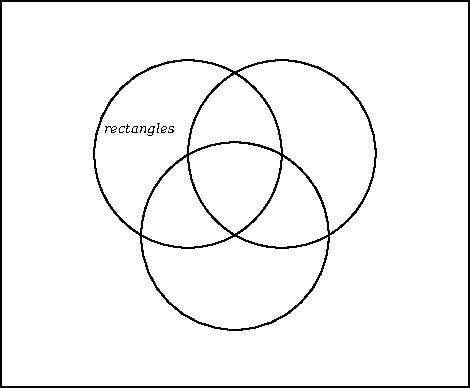
\includegraphics{../graphics/venn.pdf}
\]
\end{prob}

\begin{prob} 
Critique the task above based on mathematical content.
\end{prob}

\newpage 
\begin{prob}
Supposing we know that a quadrilateral is a polygon with four sides, write clear and succinct definitions of each of the following terms: 
\begin{enumerate}
\itemsep18pt
\item A \textit{rectangle} is a quadrilateral 
\item A \textit{parallelogram} is a quadrilateral
\item A \textit{rhombus} is a quadrilateral
\item A \textit{square} is a quadrilateral
\item A \textit{trapezoid} is a quadrilateral
\item A \textit{kite} is a quadrilateral
\end{enumerate}
\end{prob}
\bigskip

\begin{prob} 
Create a Venn diagram showing the correct relationships
among these quadrilaterals. Be ready to present and defend your
diagram to your peers.
\end{prob}

%\documentclass[handout]{ximera}
\documentclass[nooutcomes]{ximera}

\usepackage{gensymb}
\usepackage{tabularx}
\usepackage{mdframed}
\usepackage{pdfpages}
%\usepackage{chngcntr}

\let\problem\relax
\let\endproblem\relax

\newcommand{\property}[2]{#1#2}




\newtheoremstyle{SlantTheorem}{\topsep}{\fill}%%% space between body and thm
 {\slshape}                      %%% Thm body font
 {}                              %%% Indent amount (empty = no indent)
 {\bfseries\sffamily}            %%% Thm head font
 {}                              %%% Punctuation after thm head
 {3ex}                           %%% Space after thm head
 {\thmname{#1}\thmnumber{ #2}\thmnote{ \bfseries(#3)}} %%% Thm head spec
\theoremstyle{SlantTheorem}
\newtheorem{problem}{Problem}[]

%\counterwithin*{problem}{section}



%%%%%%%%%%%%%%%%%%%%%%%%%%%%Jenny's code%%%%%%%%%%%%%%%%%%%%

%%% Solution environment
%\newenvironment{solution}{
%\ifhandout\setbox0\vbox\bgroup\else
%\begin{trivlist}\item[\hskip \labelsep\small\itshape\bfseries Solution\hspace{2ex}]
%\par\noindent\upshape\small
%\fi}
%{\ifhandout\egroup\else
%\end{trivlist}
%\fi}
%
%
%%% instructorIntro environment
%\ifhandout
%\newenvironment{instructorIntro}[1][false]%
%{%
%\def\givenatend{\boolean{#1}}\ifthenelse{\boolean{#1}}{\begin{trivlist}\item}{\setbox0\vbox\bgroup}{}
%}
%{%
%\ifthenelse{\givenatend}{\end{trivlist}}{\egroup}{}
%}
%\else
%\newenvironment{instructorIntro}[1][false]%
%{%
%  \ifthenelse{\boolean{#1}}{\begin{trivlist}\item[\hskip \labelsep\bfseries Instructor Notes:\hspace{2ex}]}
%{\begin{trivlist}\item[\hskip \labelsep\bfseries Instructor Notes:\hspace{2ex}]}
%{}
%}
%% %% line at the bottom} 
%{\end{trivlist}\par\addvspace{.5ex}\nobreak\noindent\hung} 
%\fi
%
%


\let\instructorNotes\relax
\let\endinstructorNotes\relax
%%% instructorNotes environment
\ifhandout
\newenvironment{instructorNotes}[1][false]%
{%
\def\givenatend{\boolean{#1}}\ifthenelse{\boolean{#1}}{\begin{trivlist}\item}{\setbox0\vbox\bgroup}{}
}
{%
\ifthenelse{\givenatend}{\end{trivlist}}{\egroup}{}
}
\else
\newenvironment{instructorNotes}[1][false]%
{%
  \ifthenelse{\boolean{#1}}{\begin{trivlist}\item[\hskip \labelsep\bfseries {\Large Instructor Notes: \\} \hspace{\textwidth} ]}
{\begin{trivlist}\item[\hskip \labelsep\bfseries {\Large Instructor Notes: \\} \hspace{\textwidth} ]}
{}
}
{\end{trivlist}}
\fi


%% Suggested Timing
\newcommand{\timing}[1]{{\bf Suggested Timing: \hspace{2ex}} #1}




\hypersetup{
    colorlinks=true,       % false: boxed links; true: colored links
    linkcolor=blue,          % color of internal links (change box color with linkbordercolor)
    citecolor=green,        % color of links to bibliography
    filecolor=magenta,      % color of file links
    urlcolor=cyan           % color of external links
}

\title{About Sets}
\author{Bart Snapp and Brad Findell}

\outcome{Learning outcome goes here.}

\begin{document}
\begin{abstract}
  We study sets, fundamental objects in mathematics.
\end{abstract}
\maketitle

In this activity, we remind ourselves of the language and notation of sets.  In school mathematics, we often talk about sets of numbers, sets of points, sets of geometric objects, sets of functions, and even sets of sets.  When listing elements of a set, we usually enclose them in curly brackets $\{\dots\}$, and separate them with commas. 


\begin{problem}
Let $A=\text{the set of divisors of 24}$, and let $B=\text{the set of divisors of 32}$.  
\begin{enumerate}
\item Use set notation to list the elements of $A$.  
\vfill
\item Use the the symbols $\in$ (is an element of) and $\subset$ (is a subset of) to make some true statements about set $A$. 
\vspace{0.3in}
\item Draw a Venn diagram showing sets $A$ and $B$ and the relationship between them.  
\vspace{1.5in}
\end{enumerate}
\end{problem}

\begin{problem}
The notation $A\cup B$ means the \emph{union} of sets $A$ and $B$, which is to say the set of elements that are in $A$ \textbf{or} in $B$.  (Note: In mathematics, the word ``or'' is used ``inclusively.'') 

$A\cup B = $ 
\vfill
\end{problem}

\begin{problem}
The notation $A\cap B$ means the \emph{intersection} of sets $A$ and $B$, which is to say the set of elements that are in $A$ \textbf{and} in $B$. 

$A\cap B = $
\vfill
\end{problem}

\begin{problem}
Suppose $C = \{5,7,13\}$ and $D = \{6,12\}$.  
\begin{enumerate}
\item What is $C\cap D$?  Does the term \emph{empty set} help?  How should it be notated?
\vspace{0.3in}
\item Two sets with an empty intersection are said to be \emph{disjoint}.  How might you notice disjoint sets on a Venn diagram?  
\vspace{0.5in}
\item Draw a Venn diagram showing sets $A$, $B$, $C$, and $D$. 
\vspace{1in}
\end{enumerate}
\end{problem}


\end{document}


%\documentclass[handout]{ximera}
\documentclass[nooutcomes]{ximera}

\usepackage{gensymb}
\usepackage{tabularx}
\usepackage{mdframed}
\usepackage{pdfpages}
%\usepackage{chngcntr}

\let\problem\relax
\let\endproblem\relax

\newcommand{\property}[2]{#1#2}




\newtheoremstyle{SlantTheorem}{\topsep}{\fill}%%% space between body and thm
 {\slshape}                      %%% Thm body font
 {}                              %%% Indent amount (empty = no indent)
 {\bfseries\sffamily}            %%% Thm head font
 {}                              %%% Punctuation after thm head
 {3ex}                           %%% Space after thm head
 {\thmname{#1}\thmnumber{ #2}\thmnote{ \bfseries(#3)}} %%% Thm head spec
\theoremstyle{SlantTheorem}
\newtheorem{problem}{Problem}[]

%\counterwithin*{problem}{section}



%%%%%%%%%%%%%%%%%%%%%%%%%%%%Jenny's code%%%%%%%%%%%%%%%%%%%%

%%% Solution environment
%\newenvironment{solution}{
%\ifhandout\setbox0\vbox\bgroup\else
%\begin{trivlist}\item[\hskip \labelsep\small\itshape\bfseries Solution\hspace{2ex}]
%\par\noindent\upshape\small
%\fi}
%{\ifhandout\egroup\else
%\end{trivlist}
%\fi}
%
%
%%% instructorIntro environment
%\ifhandout
%\newenvironment{instructorIntro}[1][false]%
%{%
%\def\givenatend{\boolean{#1}}\ifthenelse{\boolean{#1}}{\begin{trivlist}\item}{\setbox0\vbox\bgroup}{}
%}
%{%
%\ifthenelse{\givenatend}{\end{trivlist}}{\egroup}{}
%}
%\else
%\newenvironment{instructorIntro}[1][false]%
%{%
%  \ifthenelse{\boolean{#1}}{\begin{trivlist}\item[\hskip \labelsep\bfseries Instructor Notes:\hspace{2ex}]}
%{\begin{trivlist}\item[\hskip \labelsep\bfseries Instructor Notes:\hspace{2ex}]}
%{}
%}
%% %% line at the bottom} 
%{\end{trivlist}\par\addvspace{.5ex}\nobreak\noindent\hung} 
%\fi
%
%


\let\instructorNotes\relax
\let\endinstructorNotes\relax
%%% instructorNotes environment
\ifhandout
\newenvironment{instructorNotes}[1][false]%
{%
\def\givenatend{\boolean{#1}}\ifthenelse{\boolean{#1}}{\begin{trivlist}\item}{\setbox0\vbox\bgroup}{}
}
{%
\ifthenelse{\givenatend}{\end{trivlist}}{\egroup}{}
}
\else
\newenvironment{instructorNotes}[1][false]%
{%
  \ifthenelse{\boolean{#1}}{\begin{trivlist}\item[\hskip \labelsep\bfseries {\Large Instructor Notes: \\} \hspace{\textwidth} ]}
{\begin{trivlist}\item[\hskip \labelsep\bfseries {\Large Instructor Notes: \\} \hspace{\textwidth} ]}
{}
}
{\end{trivlist}}
\fi


%% Suggested Timing
\newcommand{\timing}[1]{{\bf Suggested Timing: \hspace{2ex}} #1}




\hypersetup{
    colorlinks=true,       % false: boxed links; true: colored links
    linkcolor=blue,          % color of internal links (change box color with linkbordercolor)
    citecolor=green,        % color of links to bibliography
    filecolor=magenta,      % color of file links
    urlcolor=cyan           % color of external links
}

\title{Measuring Area}
\author{Bart Snapp and Brad Findell}

\outcome{Learning outcome goes here.}

\begin{document}
\begin{abstract}
  We measure the area of triangles.
\end{abstract}
\maketitle


\begin{teachingnote}
Supplies: Bring extra copies of the sheet (for restarting after mistakes).  Bring extra rulers. 

Nominally, this activity is about verifying that the triangle area formula gives the same result no matter which
side is chosen as the ``base.''  But the activity also allows some other challenges to come to the surface:  
\begin{itemize}
\item Some students do not realize that sometimes the line containing the base must be 
extended to allow the height to be drawn. 
\item Some students have trouble drawing a perpendicular line when the given line is neither vertical nor 
horizontal on the page.  Conceptually, this is an opportunity to highlight the definition of right angle:  An angle formed when two lines intersect so that adjacent angles are congruent.  Mechanically, students can take advantage of the fact that the tick marks on 
a ruler are perpendicular to the edge of the ruler.  
\item Some students have trouble measuring fractions of inches, sometimes thinking that the tick marks are tenths.  
\end{itemize}
\end{teachingnote}


\begin{problem}
Three congruent triangles are shown below.   
\begin{enumerate}
\item For each triangle, choose a base and use a ruler to draw carefully the corresponding height to that base.  (Choose bases of different lengths.)  Remember:  A \emph{height} is measured on a line that is perpendicular to a base and containing the opposite vertex. 
\item Measure the heights and bases accurately, and compute the area of each triangle.  
\item What do your results demonstrate about the formula for the area of a triangle?  
\end{enumerate}

\begin{image}
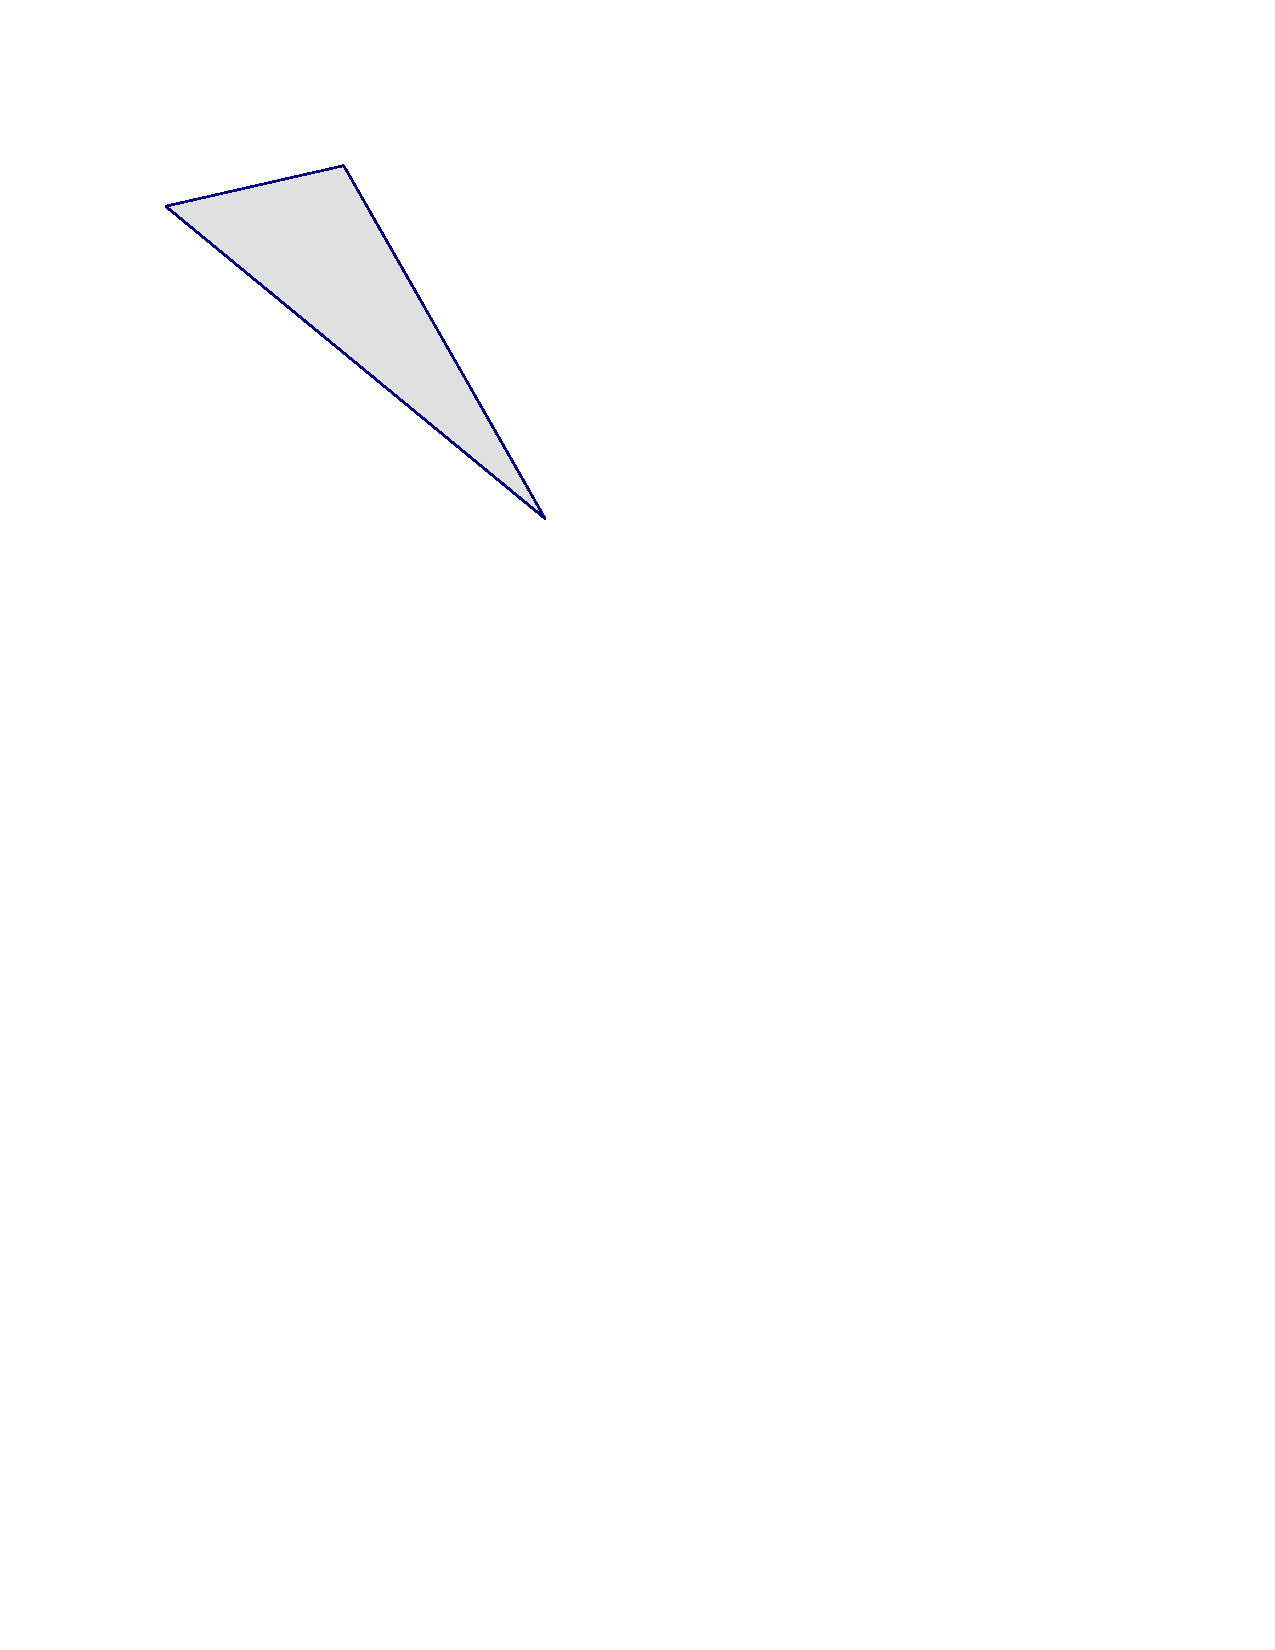
\includegraphics{triangle.pdf}
\end{image}
\begin{image}
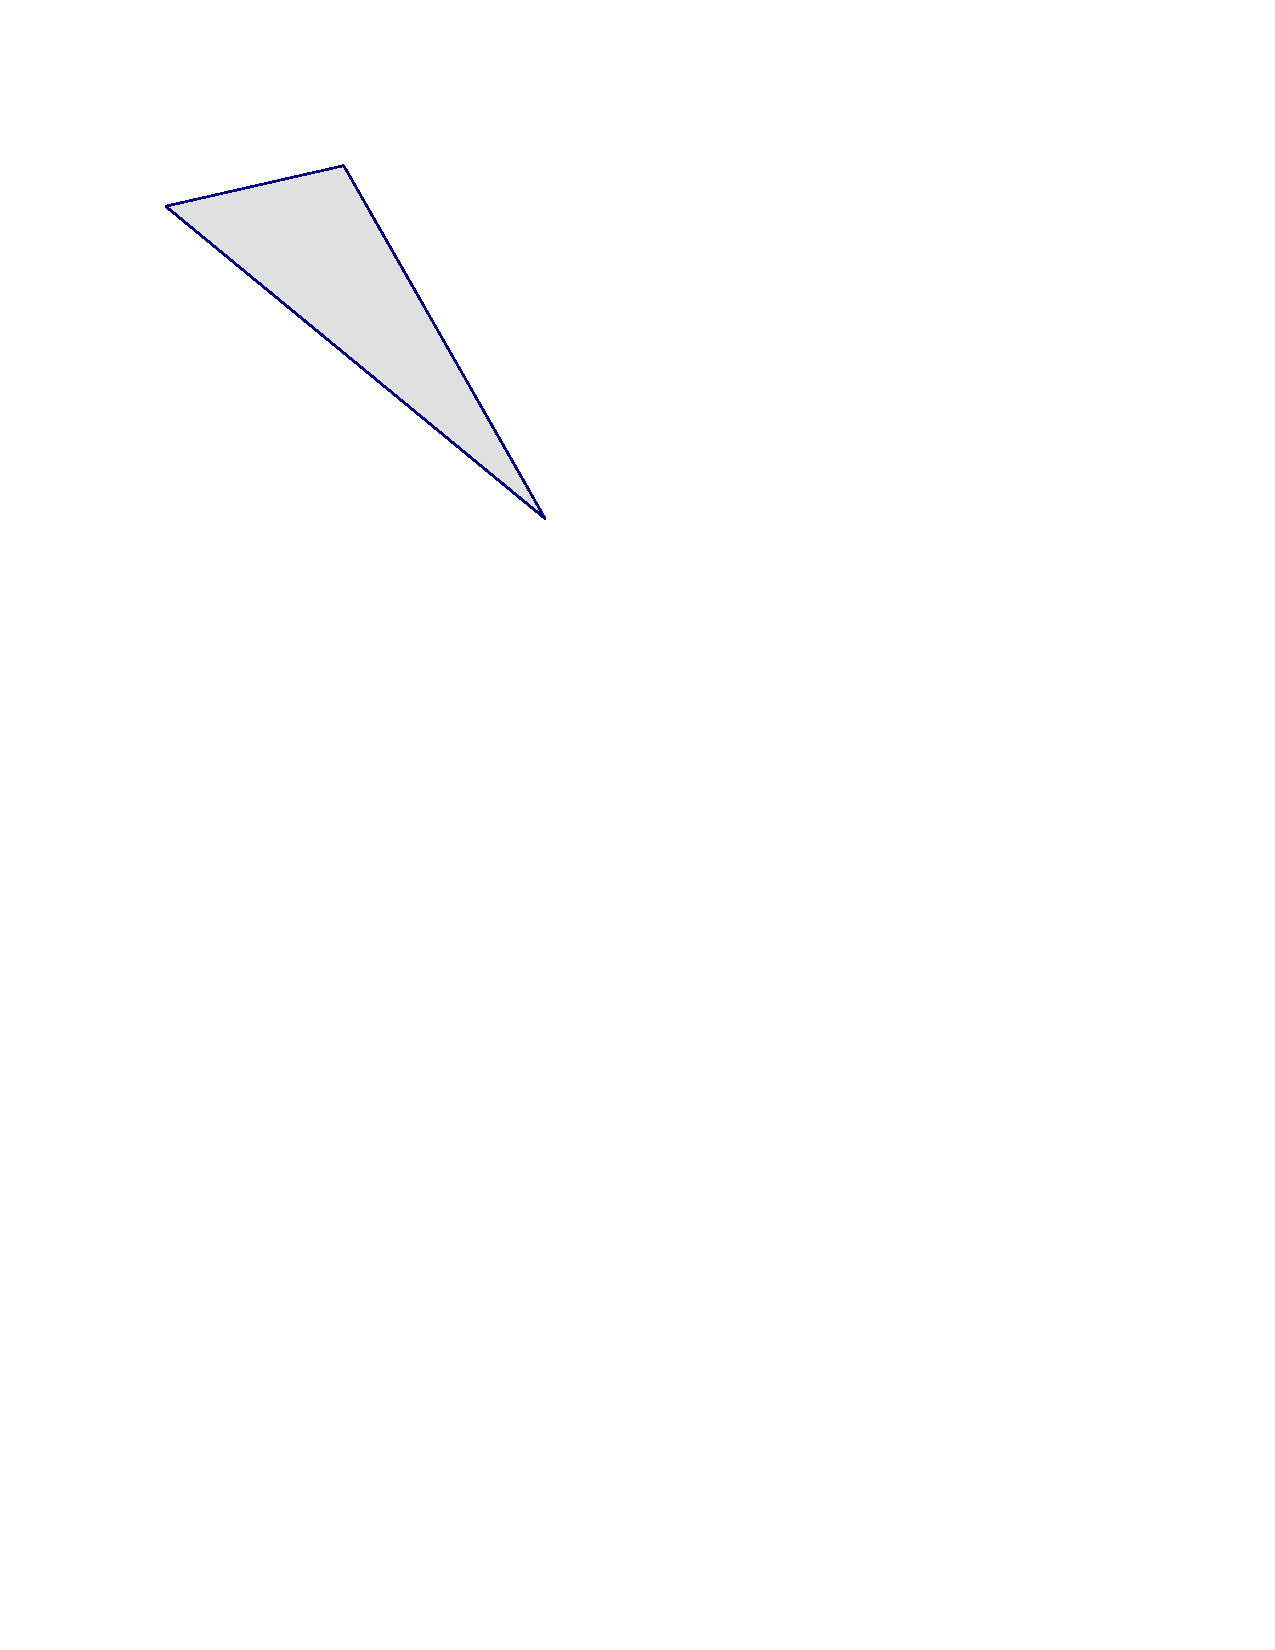
\includegraphics{triangle.pdf}
\end{image}
\begin{image}
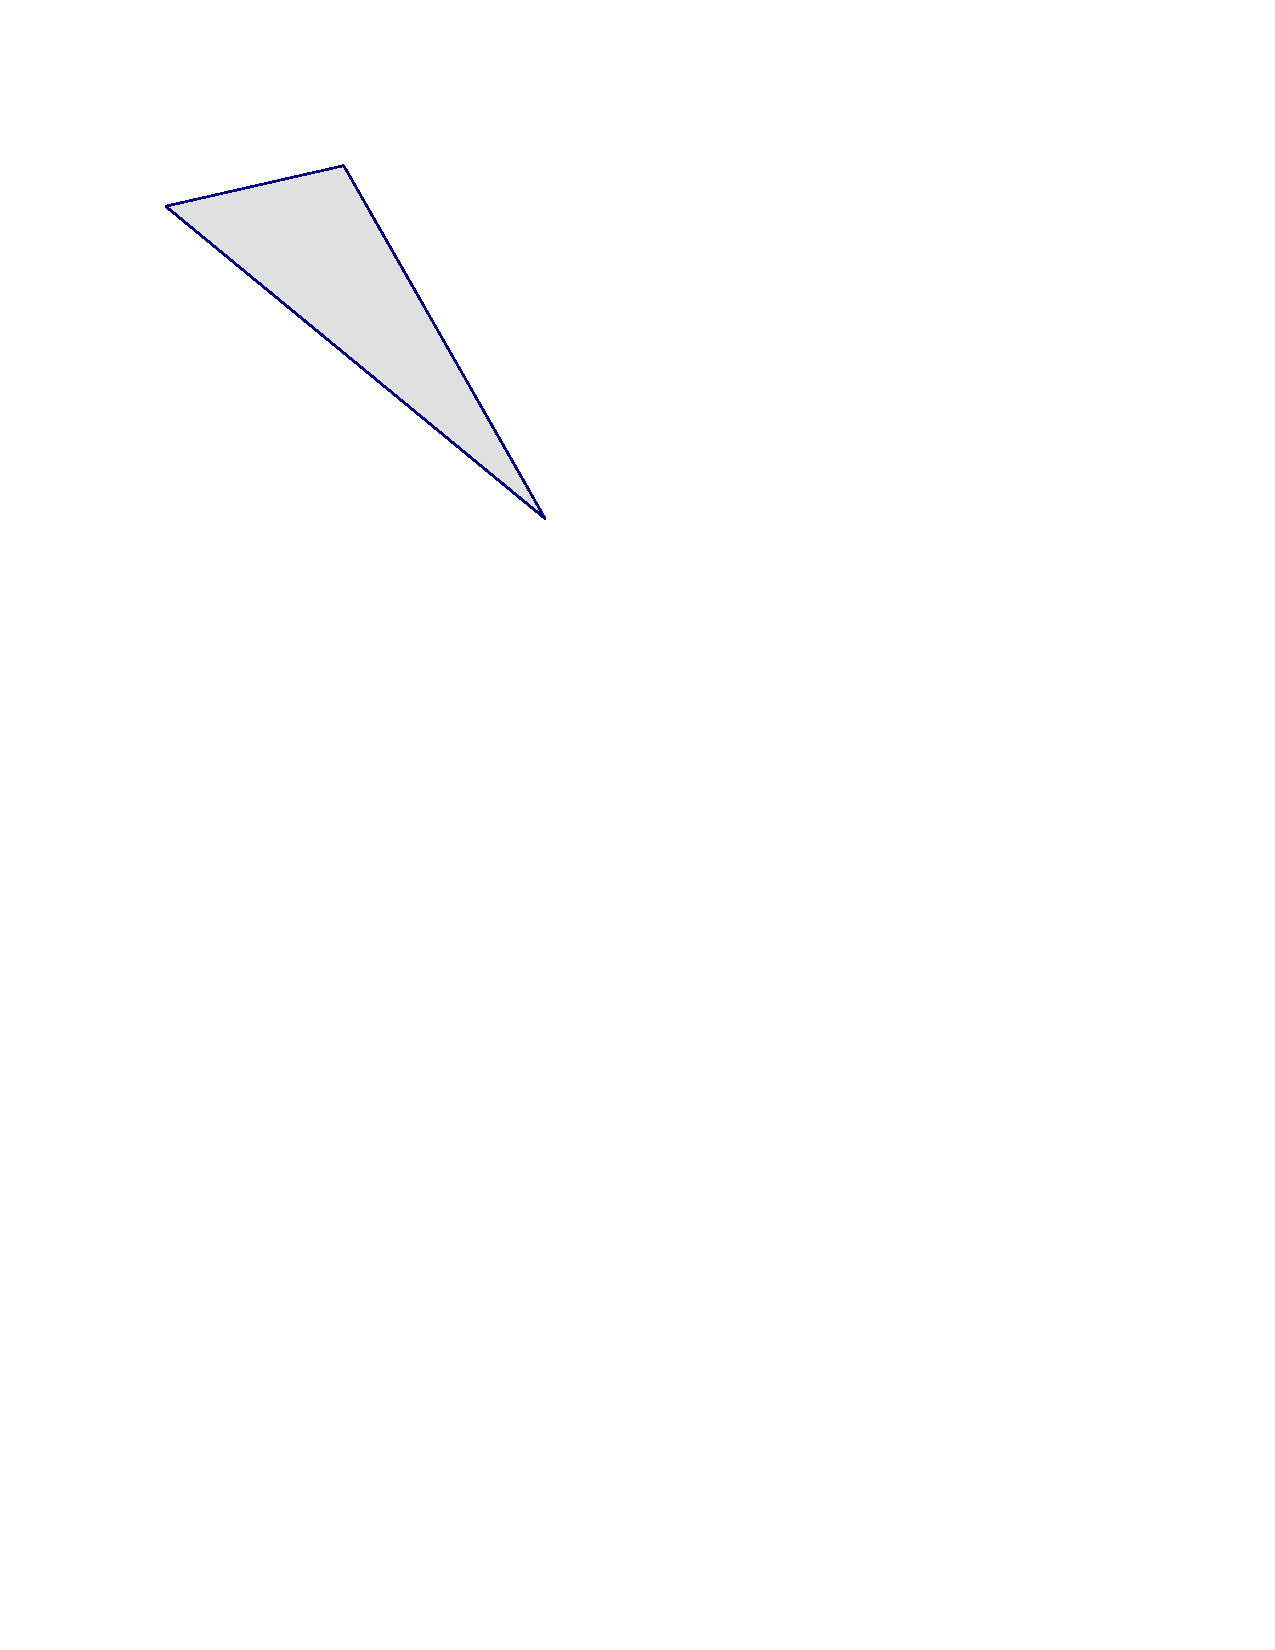
\includegraphics{triangle.pdf}
\end{image}

\end{problem}
\end{document}

\documentclass[handout]{ximera}
%\documentclass[nooutcomes,instructornotes]{ximera}

\usepackage{gensymb}
\usepackage{tabularx}
\usepackage{mdframed}
\usepackage{pdfpages}
%\usepackage{chngcntr}

\let\problem\relax
\let\endproblem\relax

\newcommand{\property}[2]{#1#2}




\newtheoremstyle{SlantTheorem}{\topsep}{\fill}%%% space between body and thm
 {\slshape}                      %%% Thm body font
 {}                              %%% Indent amount (empty = no indent)
 {\bfseries\sffamily}            %%% Thm head font
 {}                              %%% Punctuation after thm head
 {3ex}                           %%% Space after thm head
 {\thmname{#1}\thmnumber{ #2}\thmnote{ \bfseries(#3)}} %%% Thm head spec
\theoremstyle{SlantTheorem}
\newtheorem{problem}{Problem}[]

%\counterwithin*{problem}{section}



%%%%%%%%%%%%%%%%%%%%%%%%%%%%Jenny's code%%%%%%%%%%%%%%%%%%%%

%%% Solution environment
%\newenvironment{solution}{
%\ifhandout\setbox0\vbox\bgroup\else
%\begin{trivlist}\item[\hskip \labelsep\small\itshape\bfseries Solution\hspace{2ex}]
%\par\noindent\upshape\small
%\fi}
%{\ifhandout\egroup\else
%\end{trivlist}
%\fi}
%
%
%%% instructorIntro environment
%\ifhandout
%\newenvironment{instructorIntro}[1][false]%
%{%
%\def\givenatend{\boolean{#1}}\ifthenelse{\boolean{#1}}{\begin{trivlist}\item}{\setbox0\vbox\bgroup}{}
%}
%{%
%\ifthenelse{\givenatend}{\end{trivlist}}{\egroup}{}
%}
%\else
%\newenvironment{instructorIntro}[1][false]%
%{%
%  \ifthenelse{\boolean{#1}}{\begin{trivlist}\item[\hskip \labelsep\bfseries Instructor Notes:\hspace{2ex}]}
%{\begin{trivlist}\item[\hskip \labelsep\bfseries Instructor Notes:\hspace{2ex}]}
%{}
%}
%% %% line at the bottom} 
%{\end{trivlist}\par\addvspace{.5ex}\nobreak\noindent\hung} 
%\fi
%
%


\let\instructorNotes\relax
\let\endinstructorNotes\relax
%%% instructorNotes environment
\ifhandout
\newenvironment{instructorNotes}[1][false]%
{%
\def\givenatend{\boolean{#1}}\ifthenelse{\boolean{#1}}{\begin{trivlist}\item}{\setbox0\vbox\bgroup}{}
}
{%
\ifthenelse{\givenatend}{\end{trivlist}}{\egroup}{}
}
\else
\newenvironment{instructorNotes}[1][false]%
{%
  \ifthenelse{\boolean{#1}}{\begin{trivlist}\item[\hskip \labelsep\bfseries {\Large Instructor Notes: \\} \hspace{\textwidth} ]}
{\begin{trivlist}\item[\hskip \labelsep\bfseries {\Large Instructor Notes: \\} \hspace{\textwidth} ]}
{}
}
{\end{trivlist}}
\fi


%% Suggested Timing
\newcommand{\timing}[1]{{\bf Suggested Timing: \hspace{2ex}} #1}




\hypersetup{
    colorlinks=true,       % false: boxed links; true: colored links
    linkcolor=blue,          % color of internal links (change box color with linkbordercolor)
    citecolor=green,        % color of links to bibliography
    filecolor=magenta,      % color of file links
    urlcolor=cyan           % color of external links
}

\title{Suitable Precision in Language and Notation}
\author{Bart Snapp and Brad Findell}

\outcome{Learning outcome goes here.}

\begin{document}
\begin{abstract}
  We discuss language for talking about geometry.
\end{abstract}
\maketitle

Geometry is about points, lines, and other figures made up of points.  Geometric objects are sets of points.  Points can have coordinates, which are numbers, but we save these approaches for later in the course.  

Even without coordinates, geometry involves numbers because geometric objects often have length, angle measure, or area.  These are measurements:  numbers combined with units.  

The symbol $\cong$ means \emph{congruent}, which (for now) means ``has the same measure as.''  (Later, we will use transformations to define congruence.)

For now, we need some notational conventions: 

\begin{itemize}
\item $\overleftrightarrow{XY}$ denotes the \emph{line} containing $X$ and $Y$, extending indefinitely in both directions. 
\item $\overline{XY}$ denotes the \emph{line segment} from $X$ to $Y$.  Both $X$ and $Y$ are called \emph{endpoints} of the segment. 
\item $\overrightarrow{XY}$ denotes the \emph{ray} from $X$ through $Y$, and $X$ is called the \emph{endpoint} of the ray. 
\item $XY$ denotes the length of the line segment $\overline{XY}$, which is also the distance from $X$ to $Y$.  
\end{itemize}

We will find it useful to adopt the following conventions in our use of letters: 
\begin{itemize}
\item Points are usually denoted with capital letters.  
\item When a single letter is used to denote a line or segment, a lower case letters is usually used.  
\item When a single letter is used to denote an angle, a Greek letter is sometimes used.   
\end{itemize}

\textbf{Note: In general, $A\ne a \ne \alpha$. Be sure to distinguish between these types of letters!}.  

\newpage 

\begin{teachingnote}
The first two questions are about the distinction between a segment, which is a set of points, and its length, which is a measurement. 
\end{teachingnote}

\begin{problem}
Let $M$ be the midpoint of $\overline{AB}$.   
\[
\definecolor{qqqqff}{rgb}{0.,0.,1.}
\begin{tikzpicture}[line cap=round,line join=round,>=triangle 45,x=1.0cm,y=1.0cm]
\clip(-0.5,-0.4) rectangle (5,0.15);
\draw [line width=0.8pt] (0.,0.)-- (4.,0.);
%\draw [line width=0.8pt] (2.,0.)-- (1.,0.);
\draw [fill=qqqqff] (0.,0.) circle (1.2pt);
\draw[color=qqqqff] (-0.16,-0.17) node {$A$};
\draw [fill=qqqqff] (4.,0.) circle (1.2pt);
\draw[color=qqqqff] (4.14,-0.17) node {$B$};
\draw [fill=qqqqff] (2.,0.) circle (1.2pt);
\draw[color=qqqqff] (2,-0.20) node {$M$};
\end{tikzpicture}
\]
Mark each statement T (true) or F (false).  Briefly explain your reasoning.
\begin{enumerate}
\item $\overline{AB} = \overline{BA}$
\item $AB = BA$
\item $\overline{AB} \cong \overline{BA}$
\item $\overline{AM} = \overline{MB}$
\item $AM = MB$
\item $\overline{AM} \cong \overline{MB}$
\end{enumerate}
\end{problem}

\begin{problem}
Describe the geometric distinction between a segment and its length.  How are the two usually denoted differently?  
\vfill
\end{problem}

\newpage

\begin{problem}
Compare $\angle CAB$ and $\angle FDE$ in the figure below.  
\[
\definecolor{qqqqff}{rgb}{0.,0.,1.}
\begin{tikzpicture}[scale=0.75,line cap=round,line join=round,>=triangle 45,x=1.0cm,y=1.0cm]
\clip(-0.5,-0.3) rectangle (14,5.6);
\draw [to-, line width=0.8pt] (1.2,4)-- (0.,1.);
\draw [-to, line width=0.8pt] (0.,1.)-- (3.6,2.2);
\draw [to-, line width=0.8pt] (7.2,5.5)-- (5.,0.);
\draw [-to, line width=0.8pt] (5.,0.)-- (11.6,2.2);
\draw [fill=qqqqff] (0.,1.) circle (1.2pt);
\draw[color=qqqqff] (-0.22,0.89) node {$A$};
\draw [fill=qqqqff] (3.,2.) circle (1.2pt);
\draw[color=qqqqff] (3.1,1.7) node {$B$};
\draw [fill=qqqqff] (1.,3.5) circle (1.2pt);
\draw[color=qqqqff] (0.8,3.7) node {$C$};
\draw [fill=qqqqff] (5.,0.) circle (1.2pt);
\draw[color=qqqqff] (4.7,-0.1) node {$D$};
\draw [fill=qqqqff] (11.,2.) circle (1.2pt);
\draw[color=qqqqff] (11.1,1.7) node {$E$};
\draw [fill=qqqqff] (7.,5.) circle (1.2pt);
\draw[color=qqqqff] (6.8,5.2) node {$F$};
\end{tikzpicture}
\]
Mark each statement T (true) or F (false).  Briefly explain your reasoning.
\begin{enumerate}
\item $\angle CAB = \angle BAC$
\item $\angle CAB = \angle FDE$
\item $m\angle CAB < m\angle FDE$
\item $m\angle CAB = m\angle FDE$
\item $m\angle CAB \cong m\angle FDE$
\end{enumerate}
\end{problem}


\begin{problem}
There are (at least) two ways of thinking about angles.  
\begin{enumerate}
\item Use precise language to describe an angle as a set of points.  
\vspace{.5in}
\item Use precise language to describe an angle as an amount of turning.  
\end{enumerate}
\vspace{.5in}
\end{problem}
\begin{teachingnote}
An angle is the union of two rays with a common endpoint, which is called the vertex of the angle.  The vertex of an angle can also be considered the center of a rotation that would map one ray that the other.  
\end{teachingnote}

\begin{problem}
Describe the geometric distinction between an angle and its measure.  How are the two usually denoted differently?  And how do your answers relate to the previous problem?  
\vspace{1in}
\end{problem}

\begin{problem}
Use your meanings for angles to improve upon the following imprecise statements. 

\vspace{0.15in}

{\renewcommand{\arraystretch}{1.5}
\begin{tabular}{|>{\centering\arraybackslash}m{4cm}|>{\centering\arraybackslash}m{9.5cm}|}\hline
Statement & Improved Version  \\\hline

\rule{0pt}{1cm}A triangle has $180^\circ$. &  \\ \hline

\rule{0pt}{1cm}A line measures $180^\circ$. &  \\ \hline

\rule{0pt}{1cm}A circle is (or has) $360^\circ$. &  \\ \hline
 \hline
\end{tabular}}
\end{problem}

\begin{teachingnote}
\begin{itemize}
\itemsep0em
\item Let students struggle to figure out what is imprecise about the statements in the problem:  degrees measure angles, not lines, not triangles, not circles. 
\item The three vertices of the triangle are vertices of the three interior angles to be measured (and then summed).  
\item As a set of points, a straight angle is a line.  But a line is not a straight angle because an angle requires a vertex.  On a line, any point may be considered the vertex of a straight angle.
\item For a circle, we need its center, which is the vertex of central angles 
that can sum to $360^\circ$.  
\item Define right angle without using degrees: Two lines intersect to form four congruent angles.  Or two congruent angles that form a straight angle.
\end{itemize}  
\end{teachingnote}

\end{document}



%\documentclass[handout]{ximera}
\documentclass{ximera}

\usepackage{gensymb}
\usepackage{tabularx}
\usepackage{mdframed}
\usepackage{pdfpages}
%\usepackage{chngcntr}

\let\problem\relax
\let\endproblem\relax

\newcommand{\property}[2]{#1#2}




\newtheoremstyle{SlantTheorem}{\topsep}{\fill}%%% space between body and thm
 {\slshape}                      %%% Thm body font
 {}                              %%% Indent amount (empty = no indent)
 {\bfseries\sffamily}            %%% Thm head font
 {}                              %%% Punctuation after thm head
 {3ex}                           %%% Space after thm head
 {\thmname{#1}\thmnumber{ #2}\thmnote{ \bfseries(#3)}} %%% Thm head spec
\theoremstyle{SlantTheorem}
\newtheorem{problem}{Problem}[]

%\counterwithin*{problem}{section}



%%%%%%%%%%%%%%%%%%%%%%%%%%%%Jenny's code%%%%%%%%%%%%%%%%%%%%

%%% Solution environment
%\newenvironment{solution}{
%\ifhandout\setbox0\vbox\bgroup\else
%\begin{trivlist}\item[\hskip \labelsep\small\itshape\bfseries Solution\hspace{2ex}]
%\par\noindent\upshape\small
%\fi}
%{\ifhandout\egroup\else
%\end{trivlist}
%\fi}
%
%
%%% instructorIntro environment
%\ifhandout
%\newenvironment{instructorIntro}[1][false]%
%{%
%\def\givenatend{\boolean{#1}}\ifthenelse{\boolean{#1}}{\begin{trivlist}\item}{\setbox0\vbox\bgroup}{}
%}
%{%
%\ifthenelse{\givenatend}{\end{trivlist}}{\egroup}{}
%}
%\else
%\newenvironment{instructorIntro}[1][false]%
%{%
%  \ifthenelse{\boolean{#1}}{\begin{trivlist}\item[\hskip \labelsep\bfseries Instructor Notes:\hspace{2ex}]}
%{\begin{trivlist}\item[\hskip \labelsep\bfseries Instructor Notes:\hspace{2ex}]}
%{}
%}
%% %% line at the bottom} 
%{\end{trivlist}\par\addvspace{.5ex}\nobreak\noindent\hung} 
%\fi
%
%


\let\instructorNotes\relax
\let\endinstructorNotes\relax
%%% instructorNotes environment
\ifhandout
\newenvironment{instructorNotes}[1][false]%
{%
\def\givenatend{\boolean{#1}}\ifthenelse{\boolean{#1}}{\begin{trivlist}\item}{\setbox0\vbox\bgroup}{}
}
{%
\ifthenelse{\givenatend}{\end{trivlist}}{\egroup}{}
}
\else
\newenvironment{instructorNotes}[1][false]%
{%
  \ifthenelse{\boolean{#1}}{\begin{trivlist}\item[\hskip \labelsep\bfseries {\Large Instructor Notes: \\} \hspace{\textwidth} ]}
{\begin{trivlist}\item[\hskip \labelsep\bfseries {\Large Instructor Notes: \\} \hspace{\textwidth} ]}
{}
}
{\end{trivlist}}
\fi


%% Suggested Timing
\newcommand{\timing}[1]{{\bf Suggested Timing: \hspace{2ex}} #1}




\hypersetup{
    colorlinks=true,       % false: boxed links; true: colored links
    linkcolor=blue,          % color of internal links (change box color with linkbordercolor)
    citecolor=green,        % color of links to bibliography
    filecolor=magenta,      % color of file links
    urlcolor=cyan           % color of external links
}

\title{Tilted Square}
\author{Bart Snapp and Brad Findell}

\outcome{Learning outcome goes here.}

\begin{document}
\begin{abstract}
Abstract goes here.  
\end{abstract}
\maketitle


\begin{teachingnote}
This leads to the Pythagorean Theorem.  A common misconception is to ``rotate'' the figure to become a $7\times 7$ square.  Look for multiple solution methods:  (1) counting approximately, (2) counting exactly, (2) additive and (3) subtractive approaches with triangles and squares.
\end{teachingnote}

\begin{problem}
In the diagram below, the dots are 1 centimeter apart, both vertically and horizontally.  The vertices of the square all lie exactly on such dots. Find the area of the square, \emph{without computing the length of the side of the square}.  Explain your method.  

\begin{image}
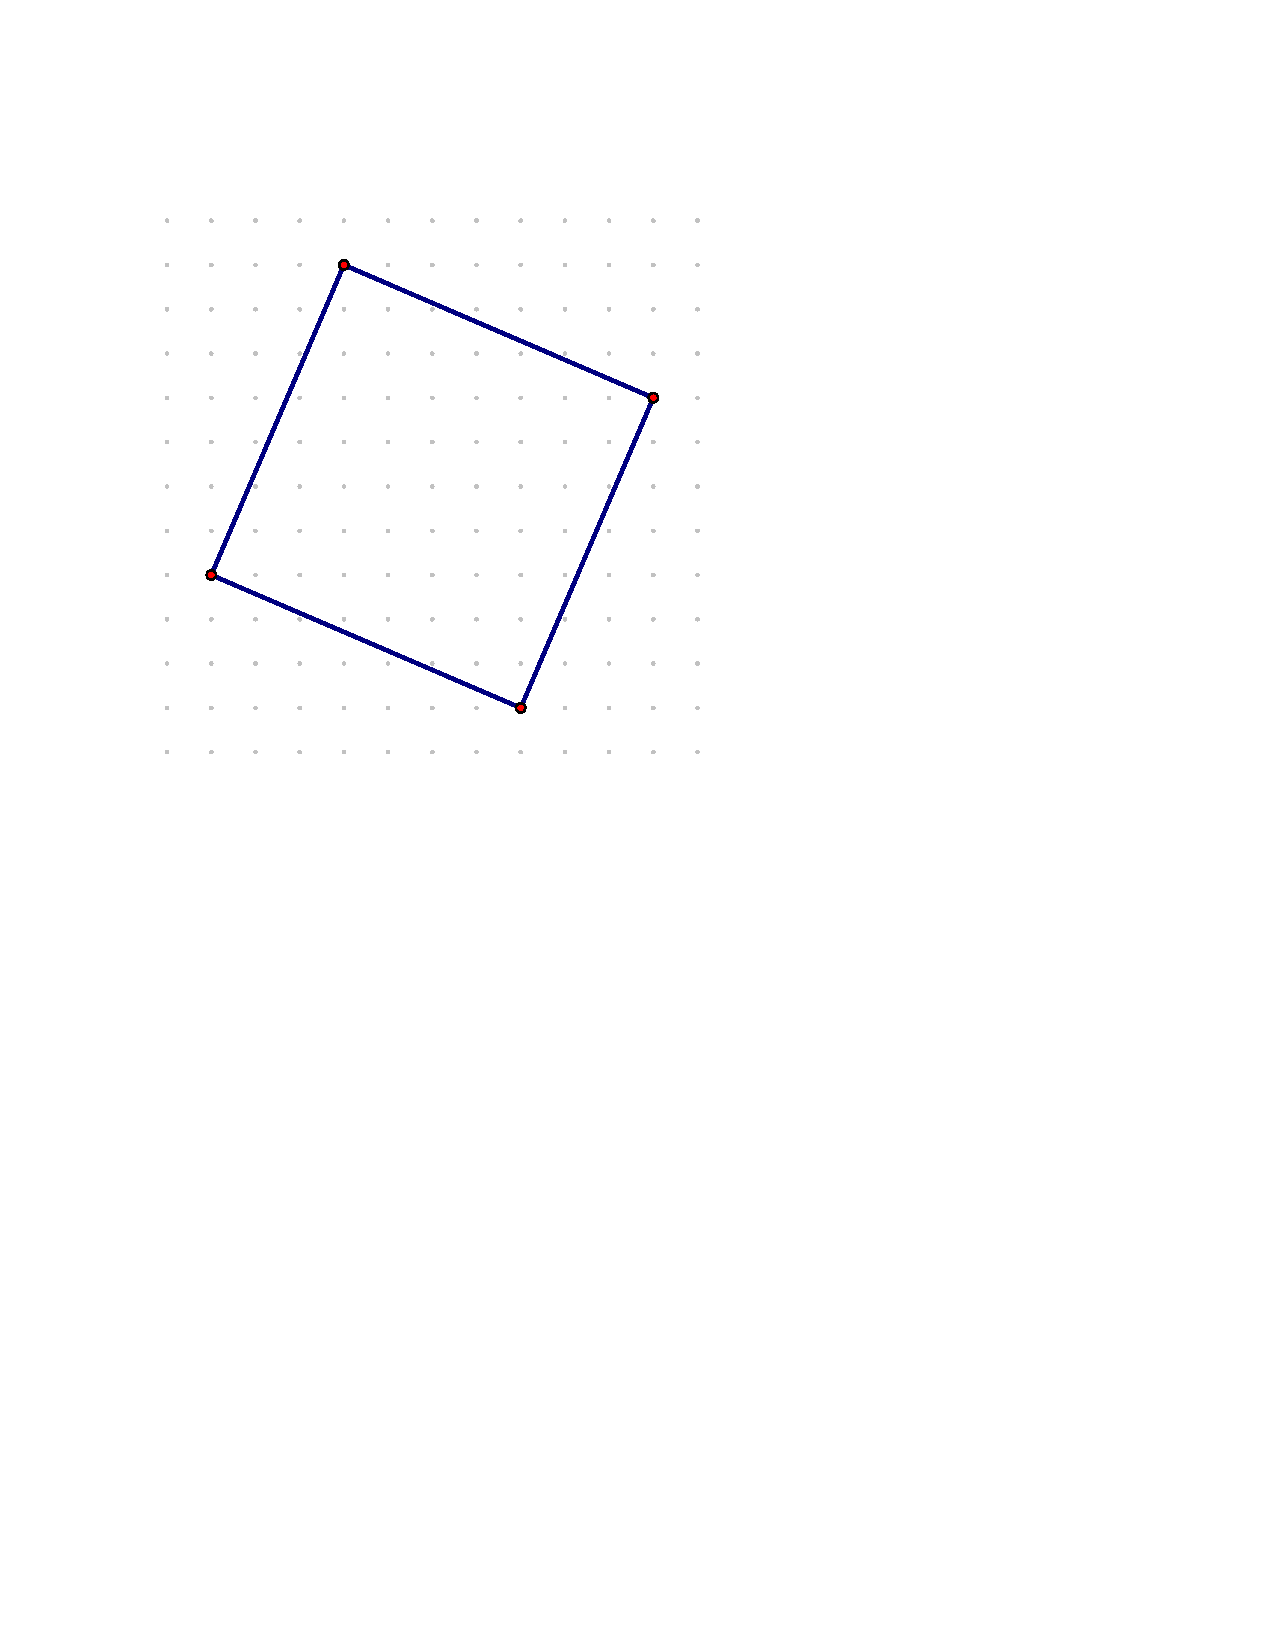
\includegraphics{tiltedSquare1.pdf}
\end{image}

\end{problem}
\end{document}
%\documentclass[handout]{ximera}
\documentclass{ximera}
\usepackage{gensymb}
\usepackage{tabularx}
\usepackage{mdframed}
\usepackage{pdfpages}
%\usepackage{chngcntr}

\let\problem\relax
\let\endproblem\relax

\newcommand{\property}[2]{#1#2}




\newtheoremstyle{SlantTheorem}{\topsep}{\fill}%%% space between body and thm
 {\slshape}                      %%% Thm body font
 {}                              %%% Indent amount (empty = no indent)
 {\bfseries\sffamily}            %%% Thm head font
 {}                              %%% Punctuation after thm head
 {3ex}                           %%% Space after thm head
 {\thmname{#1}\thmnumber{ #2}\thmnote{ \bfseries(#3)}} %%% Thm head spec
\theoremstyle{SlantTheorem}
\newtheorem{problem}{Problem}[]

%\counterwithin*{problem}{section}



%%%%%%%%%%%%%%%%%%%%%%%%%%%%Jenny's code%%%%%%%%%%%%%%%%%%%%

%%% Solution environment
%\newenvironment{solution}{
%\ifhandout\setbox0\vbox\bgroup\else
%\begin{trivlist}\item[\hskip \labelsep\small\itshape\bfseries Solution\hspace{2ex}]
%\par\noindent\upshape\small
%\fi}
%{\ifhandout\egroup\else
%\end{trivlist}
%\fi}
%
%
%%% instructorIntro environment
%\ifhandout
%\newenvironment{instructorIntro}[1][false]%
%{%
%\def\givenatend{\boolean{#1}}\ifthenelse{\boolean{#1}}{\begin{trivlist}\item}{\setbox0\vbox\bgroup}{}
%}
%{%
%\ifthenelse{\givenatend}{\end{trivlist}}{\egroup}{}
%}
%\else
%\newenvironment{instructorIntro}[1][false]%
%{%
%  \ifthenelse{\boolean{#1}}{\begin{trivlist}\item[\hskip \labelsep\bfseries Instructor Notes:\hspace{2ex}]}
%{\begin{trivlist}\item[\hskip \labelsep\bfseries Instructor Notes:\hspace{2ex}]}
%{}
%}
%% %% line at the bottom} 
%{\end{trivlist}\par\addvspace{.5ex}\nobreak\noindent\hung} 
%\fi
%
%


\let\instructorNotes\relax
\let\endinstructorNotes\relax
%%% instructorNotes environment
\ifhandout
\newenvironment{instructorNotes}[1][false]%
{%
\def\givenatend{\boolean{#1}}\ifthenelse{\boolean{#1}}{\begin{trivlist}\item}{\setbox0\vbox\bgroup}{}
}
{%
\ifthenelse{\givenatend}{\end{trivlist}}{\egroup}{}
}
\else
\newenvironment{instructorNotes}[1][false]%
{%
  \ifthenelse{\boolean{#1}}{\begin{trivlist}\item[\hskip \labelsep\bfseries {\Large Instructor Notes: \\} \hspace{\textwidth} ]}
{\begin{trivlist}\item[\hskip \labelsep\bfseries {\Large Instructor Notes: \\} \hspace{\textwidth} ]}
{}
}
{\end{trivlist}}
\fi


%% Suggested Timing
\newcommand{\timing}[1]{{\bf Suggested Timing: \hspace{2ex}} #1}




\hypersetup{
    colorlinks=true,       % false: boxed links; true: colored links
    linkcolor=blue,          % color of internal links (change box color with linkbordercolor)
    citecolor=green,        % color of links to bibliography
    filecolor=magenta,      % color of file links
    urlcolor=cyan           % color of external links
}


\outcome{Learning outcome goes here.}

\author{Bart Snapp and Brad Findell}
\title{Pythagorean Theorem}

\begin{document}
\begin{abstract}
Abstract goes here.  
\end{abstract}
\maketitle


\begin{instructorIntro}
Before problem 1, ask:  ``State the Pythagorean Theorem.''  Give students about a minute to write something down.  Many students will write only, ``$a^2 + b^2 = c^2$.''  Then in whole class discussion, draw out the missing pieces:  (1) that $a$, $b$, and $c$ are side lengths of a triangle;  (2) that the triangle is a right triangle; and (3) that $c$ is the length of the hypotenuse.  Then, the class decision can be as follows: 
 
\begin{quote}\textbf{Pythagorean Theorem:}  Suppose a triangle has side lengths $a$, $b$, and $c$.  If the triangle is right with hypotenuse $c$, then $a^2 + b^2 = c^2$. 
\end{quote}
The advantage of this phrasing is that it paves the way for a clear statement of a converse (below).   

Some students will use only the left picture and algebra (i.e., the distributive property) to get the desired result.  The advantage of both pictures is that algebra is not necessary, as the right picture provides the distributive property via rearranging the pieces.  

Once they have proven the Pythagorean Theorem for the particular triangle as drawn, ask, ``How do we know it will work for any triangle?''  The conceptual leap is that the reasoning is exactly the same.  

The term \emph{converse} may need to be introduced.  Perhaps include an example of a true statement with a false converse (e.g., about vertical angles, or about divisibility by 4 and even).  

\begin{quote}
\textbf{Converse of the Pythagorean Theorem:}  Suppose a triangle has side lengths $a$, $b$, and $c$.  If $a^2 + b^2 = c^2$, then the triangle is right with hypotenuse $c$. 
\end{quote}

For the proof, construct a separate right triangle with legs of length $a$ and $b$ and hypotenuse $d$.  By the (forward direction) of the Pythagorean Theorem, $a^2+b^2=d^2$.  (For students who find it difficult to accept this reasoning, it can help to remind them that a statement and its converse are logically distinct.)  By algebra, $c=d$.  By SSS, the two triangles are congruent, so the original triangle must be right.  

Perhaps add a problem about the history involving Egyptians, ropes, knots, and right angles.  Ask whether it is about the theorem or the converse. 
\end{instructorIntro}


\begin{problem}
Give two explanations of how the following picture ``proves''
  the Pythagorean Theorem, one using algebra and one without algebra. \fixnote{Cite CCSS 8.G.6.} % \standard{8.G.6} 
\begin{image}
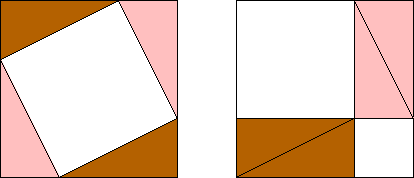
\includegraphics[scale=1.3]{./graphics/pbppyth1.pdf}
\end{image}
\end{problem}

\begin{problem}
State the converse of the Pythagorean Theorem and prove it.  
\end{problem}

\end{document}


%\newpage
\section{Louie Llama and the Triangle} 

\fixnote{Also include something like Walking and Turning from Beckmann.  Or let Louie do the walking and draw new pictures.  Supplies needed:  Tape.}

We are going to investigate why the interior angles of a triangle sum
to $180^\circ$. We won't be alone on this journey, we'll have help.
Meet Louie Llama:\index{Louie Llama}
\[
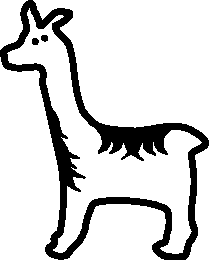
\includegraphics[height=1in]{../graphics/llama.pdf}
\]

Louie Llama is rather radical for a llama and doesn't mind being
rotated at all.

\begin{prob} 
Draw a picture of Louie Llama rotated $90^\circ$ counterclockwise.
\end{prob}

\begin{prob} 
Draw a picture of Louie Llama rotated $180^\circ$ counterclockwise.
\end{prob}

\begin{prob} 
Draw a picture of Louie Llama rotated $360^\circ$ counterclockwise.
\end{prob}

\begin{prob} Sometimes Louie Llama likes to walk around lines he finds:
\[
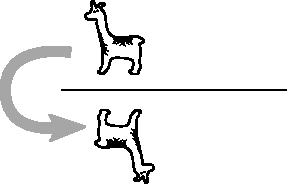
\includegraphics{../graphics/llamaLines.pdf}
\]
Through what angle did Louie Llama just rotate?
\end{prob}


Now we're going to watch Louie Llama go for a walk. Draw yourself any
triangle.  Draw a crazy scalene triangle---those are the kind that Louie
Llama likes best. Louie Llama is going to parade proudly around this
triangle. When Louie Llama walks around corners he rotates. Check
it out:
\[
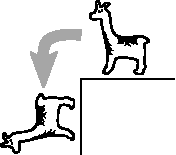
\includegraphics{../graphics/llamaCorner.pdf}
\]
\fixnote{Maybe we need a non-right angle here and later so that students can 
more easily distinguish the exterior and interior angles.}
Take your triangle and denote the measure of its angles as $a$, $b$,
and $c$. Start Louie Llama out along a side adjacent to the angle of
measure $a$. He should be on the outside of the triangle, his feet
should be pointing toward the triangle, and his face should be
pointing toward the angle of measure $b$.
\begin{prob} 
Sketch Louie Llama walking to the angle of measure $b$. Walk him
around the angle. As he goes around the angle his feet should always
be pointing toward the triangle. Through what angle did Louie Llama
just rotate?
\end{prob}

\begin{prob}
Sketch Louie Llama walking to the angle of measure $c$. Walk him
around the angle. Through what angle did Louie Llama just rotate?
\end{prob}

\begin{prob}
Finally sketch Louie Llama walking back to the angle of measure
$a$. Walk him around the angle. He should be back at his starting
point. Through what angle did Louie Llama just rotate?
\end{prob}

\begin{prob} 
All in all, how many degrees did Louie Llama rotate in his walk?
\end{prob}

\begin{prob} 
Write an equation where the right-hand side is Louie Llama's total
rotation and the left-hand side is the sum of each rotation around the
angle. Can you solve for $a+b+c$?
\end{prob}

As you may have guessed, Louie Llama isn't your typical llama, for one
thing he likes to walk backwards and on his head! He also like to do
somersaults. Louie Llama can somersault around corners in two
different ways:
\[
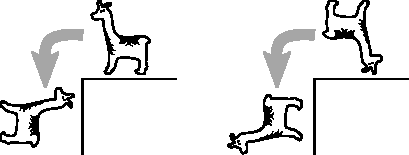
\includegraphics{../graphics/llamaSomer.pdf}
\]
\fixnote{Rotating through interior angles might be clearer, which would require new pictures, probably with non-right angles.}

\begin{prob} 
What does Louie Llama's somersault have to do with the angle of the
corner? Can you precisely explain how Louie Llama rotates when he
somersaults around corners?
\end{prob}


\begin{prob}
Can you walk Louie Llama around your original triangle allowing him to
walk backwards (or even on his head!), letting him do somersaults as
he pleases around corners, and \textbf{directly} arrive at the
equation\index{triangle!sum of interior angles}
\[
a + b + c = 180^\circ?
\]
\end{prob}

\begin{prob} 
Can you rephrase what we did above in terms of \textit{exterior angles} and \textit{interior angles}?\index{interior angles}
\end{prob}

\break

\begin{prob} 
Can you walk Louie Llama around other shapes and figure out what the
sum of their interior angles are? Let's do this with a table:\fixnote{Do we want to include exterior angles in the table?}
\[
{\renewcommand{\arraystretch}{1.5}
\begin{tabular}{|c|c|c|}\hline
$n$-gon & sum of interior angles & interior angle of a regular $n$-gon\\\hline\hline
3 & & \\\hline
4 & & \\\hline
5 & & \\\hline
6 & & \\\hline
7 & & \\\hline
8 & & \\\hline
$n$ & & \\\hline
\end{tabular}}
\]
\end{prob}


%\newpage
\section{Louie Llama and Regular Polygons} 

Louie Llama is a very curious llama.\index{Louie Llama} He knows that
each angle of a regular $3$-gon is $60^\circ$. He also knows that each
angle of a regular $4$-gon is $90^\circ$. But what he really wants to
know, are the measure of each angle of a regular $n$-gon. In this
activity we'll see if we can answer this question.


\begin{prob} 
Draw a picture of Louie Llama rotated $90^\circ$ counterclockwise.
\end{prob}

\begin{prob} 
Draw a picture of Louie Llama rotated $180^\circ$ counterclockwise.
\end{prob}

\begin{prob} 
Draw a picture of Louie Llama rotated $360^\circ$ counterclockwise.
\end{prob}

\begin{prob} Sometimes Louie Llama likes to walk around lines he finds:
\[
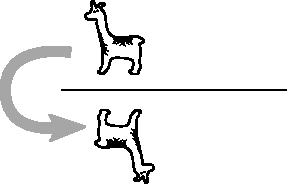
\includegraphics{../graphics/llamaLines.pdf}
\]
Through what angle did Louie Llama just rotate?
\end{prob}

Again, we're going to watch Louie Llama go for a walk. Draw yourself
any a regular $3$-gon. When Louie Llama walks around corners he
rotates. Check it out:
\[
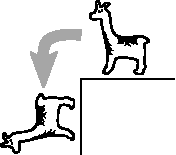
\includegraphics{../graphics/llamaCorner.pdf}
\]
Since your $3$-gon is regular, each of its angles has measure
$\theta$. 
\begin{prob} 
Sketch Louie Llama walking around our $3$-gon. As he goes around a
corner, through what angle does Louie Llama rotate?
\end{prob}

\begin{prob}
Find the measure of each angle of a $3$-gon. Explain your reasoning.
\end{prob}

\begin{prob}
Sketch a regular $4$-gon and find the measure of each angle of a
$4$-gon. Explain your reasoning.
\end{prob}


\begin{prob}
Sketch a regular $5$-gon and find the measure of each angle of a
$5$-gon. Explain your reasoning.
\end{prob}


\begin{prob}
Sketch a regular $6$-gon and find the measure of each angle of a
$6$-gon. Explain your reasoning.
\end{prob}


Now it is time to generalize!

\begin{prob}
Sketch a regular $n$-gon and find the measure of each angle of a
$n$-gon. Explain your reasoning. Note, your answer should be a formula.
\end{prob}



\newpage
\section{Angles in a Funky Shape} 

\begin{teachingnote}
Nonconvex is better than concave.  Think of the amount of turning to identify which angle they are measuring.  Accuracy of protractor measurement.  Triangulation is the point of the angle sum.  An error worth discussing is triangulating incorrectly.
\end{teachingnote}
We are going to investigate the sum of the interior angles of a
funky shape.

\begin{prob}
Using a protractor, measure the interior angles of the crazy shape below:
\vspace{0.1in}
\[
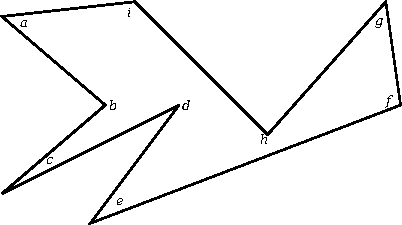
\includegraphics[scale=1.6]{../graphics/funkyshape.pdf}
\]
Use this table to record your findings:
\[
\vspace{0.1in}
{\renewcommand{\arraystretch}{1.5}
\begin{array}{|c|c|c|c|c|c|c|c|c|}\hline
a & b & c & d & e & f & g & h & i \\\hline
\rule[7mm]{10mm}{0mm}  & \rule[7mm]{10mm}{0mm}    & \rule[7mm]{10mm}{0mm}   & \rule[7mm]{10mm}{0mm}   &  \rule[7mm]{10mm}{0mm}   & \rule[7mm]{10mm}{0mm}    & \rule[7mm]{10mm}{0mm}   & \rule[7mm]{10mm}{0mm}   & \rule[7mm]{10mm}{0mm}   \\ \hline
\end{array}}
\]
\end{prob}

\begin{prob}
Find the sum of the interior angles of the polygon above. 
\end{prob}


\begin{prob}
What should the sum be? Explain your reasoning.  
(You might find it useful to consider some of the angles to be ``reflex angles.''  Which ones?)  
\end{prob}



%\documentclass[handout]{ximera}
\documentclass[nooutcomes,instructornotes]{ximera}

\usepackage{gensymb}
\usepackage{tabularx}
\usepackage{mdframed}
\usepackage{pdfpages}
%\usepackage{chngcntr}

\let\problem\relax
\let\endproblem\relax

\newcommand{\property}[2]{#1#2}




\newtheoremstyle{SlantTheorem}{\topsep}{\fill}%%% space between body and thm
 {\slshape}                      %%% Thm body font
 {}                              %%% Indent amount (empty = no indent)
 {\bfseries\sffamily}            %%% Thm head font
 {}                              %%% Punctuation after thm head
 {3ex}                           %%% Space after thm head
 {\thmname{#1}\thmnumber{ #2}\thmnote{ \bfseries(#3)}} %%% Thm head spec
\theoremstyle{SlantTheorem}
\newtheorem{problem}{Problem}[]

%\counterwithin*{problem}{section}



%%%%%%%%%%%%%%%%%%%%%%%%%%%%Jenny's code%%%%%%%%%%%%%%%%%%%%

%%% Solution environment
%\newenvironment{solution}{
%\ifhandout\setbox0\vbox\bgroup\else
%\begin{trivlist}\item[\hskip \labelsep\small\itshape\bfseries Solution\hspace{2ex}]
%\par\noindent\upshape\small
%\fi}
%{\ifhandout\egroup\else
%\end{trivlist}
%\fi}
%
%
%%% instructorIntro environment
%\ifhandout
%\newenvironment{instructorIntro}[1][false]%
%{%
%\def\givenatend{\boolean{#1}}\ifthenelse{\boolean{#1}}{\begin{trivlist}\item}{\setbox0\vbox\bgroup}{}
%}
%{%
%\ifthenelse{\givenatend}{\end{trivlist}}{\egroup}{}
%}
%\else
%\newenvironment{instructorIntro}[1][false]%
%{%
%  \ifthenelse{\boolean{#1}}{\begin{trivlist}\item[\hskip \labelsep\bfseries Instructor Notes:\hspace{2ex}]}
%{\begin{trivlist}\item[\hskip \labelsep\bfseries Instructor Notes:\hspace{2ex}]}
%{}
%}
%% %% line at the bottom} 
%{\end{trivlist}\par\addvspace{.5ex}\nobreak\noindent\hung} 
%\fi
%
%


\let\instructorNotes\relax
\let\endinstructorNotes\relax
%%% instructorNotes environment
\ifhandout
\newenvironment{instructorNotes}[1][false]%
{%
\def\givenatend{\boolean{#1}}\ifthenelse{\boolean{#1}}{\begin{trivlist}\item}{\setbox0\vbox\bgroup}{}
}
{%
\ifthenelse{\givenatend}{\end{trivlist}}{\egroup}{}
}
\else
\newenvironment{instructorNotes}[1][false]%
{%
  \ifthenelse{\boolean{#1}}{\begin{trivlist}\item[\hskip \labelsep\bfseries {\Large Instructor Notes: \\} \hspace{\textwidth} ]}
{\begin{trivlist}\item[\hskip \labelsep\bfseries {\Large Instructor Notes: \\} \hspace{\textwidth} ]}
{}
}
{\end{trivlist}}
\fi


%% Suggested Timing
\newcommand{\timing}[1]{{\bf Suggested Timing: \hspace{2ex}} #1}




\hypersetup{
    colorlinks=true,       % false: boxed links; true: colored links
    linkcolor=blue,          % color of internal links (change box color with linkbordercolor)
    citecolor=green,        % color of links to bibliography
    filecolor=magenta,      % color of file links
    urlcolor=cyan           % color of external links
}

\title{Trapezoid Area}
\author{Bart Snapp and Brad Findell}

\outcome{Learning outcome goes here.}

\begin{document}
\begin{abstract}
  We investigate trapezoids and how to compute their area.
\end{abstract}
\maketitle

\begin{teachingnote}
We set the stage with triangles.  A challenge for students is distinguishing the various `bases,' and realizing how helpful it is to label them with different letters.   
\end{teachingnote}

\begin{problem}Explain how the following picture ``proves'' that
  the area of a right triangle is half the base times the height.

\[
\definecolor{qqwuqq}{rgb}{0.,0.39215686274509803,0.}
\begin{tikzpicture}[line cap=round,line join=round,>=triangle 45,x=1.0cm,y=1.0cm]
\clip(-0.1,-0.1) rectangle (3.1,4.1);
\draw[line width=0.8pt,color=qqwuqq,fill=qqwuqq,fill opacity=0.10] (0.2828,0.) -- (0.2828,0.2828) -- (0.,0.2828) -- (0.,0.) -- cycle; 
\draw [line width=0.8pt] (0.,4.)-- (0.,0.);
\draw [line width=0.8pt] (0.,0.)-- (3.,0.);
\draw [line width=0.8pt] (3.,0.)-- (0.,4.);
\draw [line width=0.8pt,dash pattern=on 2pt off 2pt] (0.,4.)-- (3.,4.);
\draw [line width=0.8pt,dash pattern=on 2pt off 2pt] (3.,4.)-- (3.,0.);
\end{tikzpicture}
\]
%
%\[
%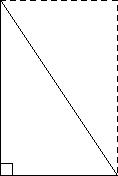
\includegraphics[scale=0.8]{pbpAreaRight.pdf}
%\]
\end{problem}

\begin{problem} Suppose you know that the area of a \textbf{right} triangle is
  half the base times the height. Explain how the following picture
  ``proves'' that the area of \textbf{every} triangle is half the base times the
  height.
\[
\definecolor{qqwuqq}{rgb}{0.,0.392,0.}
\begin{tikzpicture}[line cap=round,line join=round,>=triangle 45,x=1.0cm,y=1.0cm]
\clip(-0.5,-0.05) rectangle (5,2.55);
\draw[line width=0.8pt,color=qqwuqq,fill=qqwuqq,fill opacity=0.1] (3.,0.1954) -- (2.8046,0.1954) -- (2.8046,0.) -- (3.,0.) -- cycle; 
\draw[line width=0.8pt,color=qqwuqq,fill=qqwuqq,fill opacity=0.1] (3.1954,0.) -- (3.1954,0.1954) -- (3.,0.1954) -- (3.,0.) -- cycle; 
\draw [line width=0.8pt] (0.,0.)-- (3.,2.5);
\draw [line width=0.8pt] (3.,2.5)-- (4.,0.);
\draw [line width=0.8pt] (4.,0.)-- (0.,0.);
\draw [line width=0.8pt] (0.,0.)-- (3.,0.);
\draw [line width=0.8pt] (3.,0.)-- (4.,0.);
\draw [line width=0.8pt,dash pattern=on 2pt off 2pt] (3.,0.)-- (3.,2.5);
\end{tikzpicture}
\]
%\[
%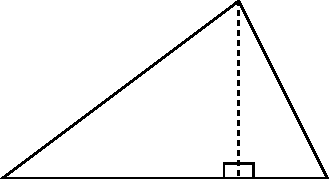
\includegraphics[scale=0.8]{../graphics/pbpDisTri.pdf}
%\]
\vspace{1in}
\end{problem}

\begin{problem}
Now suppose that \textit{Geometry Giorgio} attempts to
solve a similar problem. Again knowing that the area of a right
triangle is half the base times the height, he draws the following
picture:
\[
\begin{tikzpicture}[line cap=round,line join=round,>=triangle 45,x=1.0cm,y=1.0cm]
\clip(-0.5,-0.05) rectangle (5.25,2.55);
\draw [line width=0.8pt,dash pattern=on 2pt off 2pt] (0.,0.)-- (0.,2.5);
\draw [line width=0.8pt,dash pattern=on 2pt off 2pt] (0.,2.5)-- (5.,2.5);
\draw [line width=0.8pt,dash pattern=on 2pt off 2pt] (5.,2.5)-- (5.,0.);
\draw [line width=0.8pt] (5.,2.5)-- (2.,0.);
\draw [line width=0.8pt] (5.,2.5)-- (0.,0.);
\draw [line width=0.8pt] (0.,0.)-- (2.,0.);
\draw [line width=0.8pt,dash pattern=on 2pt off 2pt] (2.,0.)-- (5.,0.);
\end{tikzpicture}
\]
%\[
%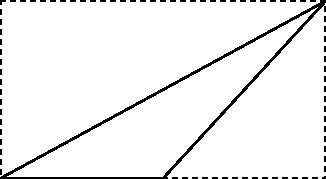
\includegraphics[scale=0.8]{../graphics/pbpDisTriGio.pdf}
%\]
\textit{Geometry Giorgio} states that the diagonal line cuts the
rectangle in half, and thus the area of the triangle is half the base
times the height. Is this correct reasoning? If so, give a complete
explanation. If not, give correct reasoning based on \textit{Geometry
  Giorgio}'s picture.
\vspace{2in}
\end{problem}

\begin{teachingnote}
The point of the next problem is connecting the geometric thinking with the algebraic thinking.  For example, how, algebraically and geometrically, does the first trapezoid formula look like an average?  In the last problem, students might not see the similar triangles.

Another approach, not included here: ``A rectangle plus two triangles.''
\end{teachingnote}


\begin{problem}
Now we explore several ways of justifying the formula for the area of a trapezoid, as labeled below. 
\begin{image}
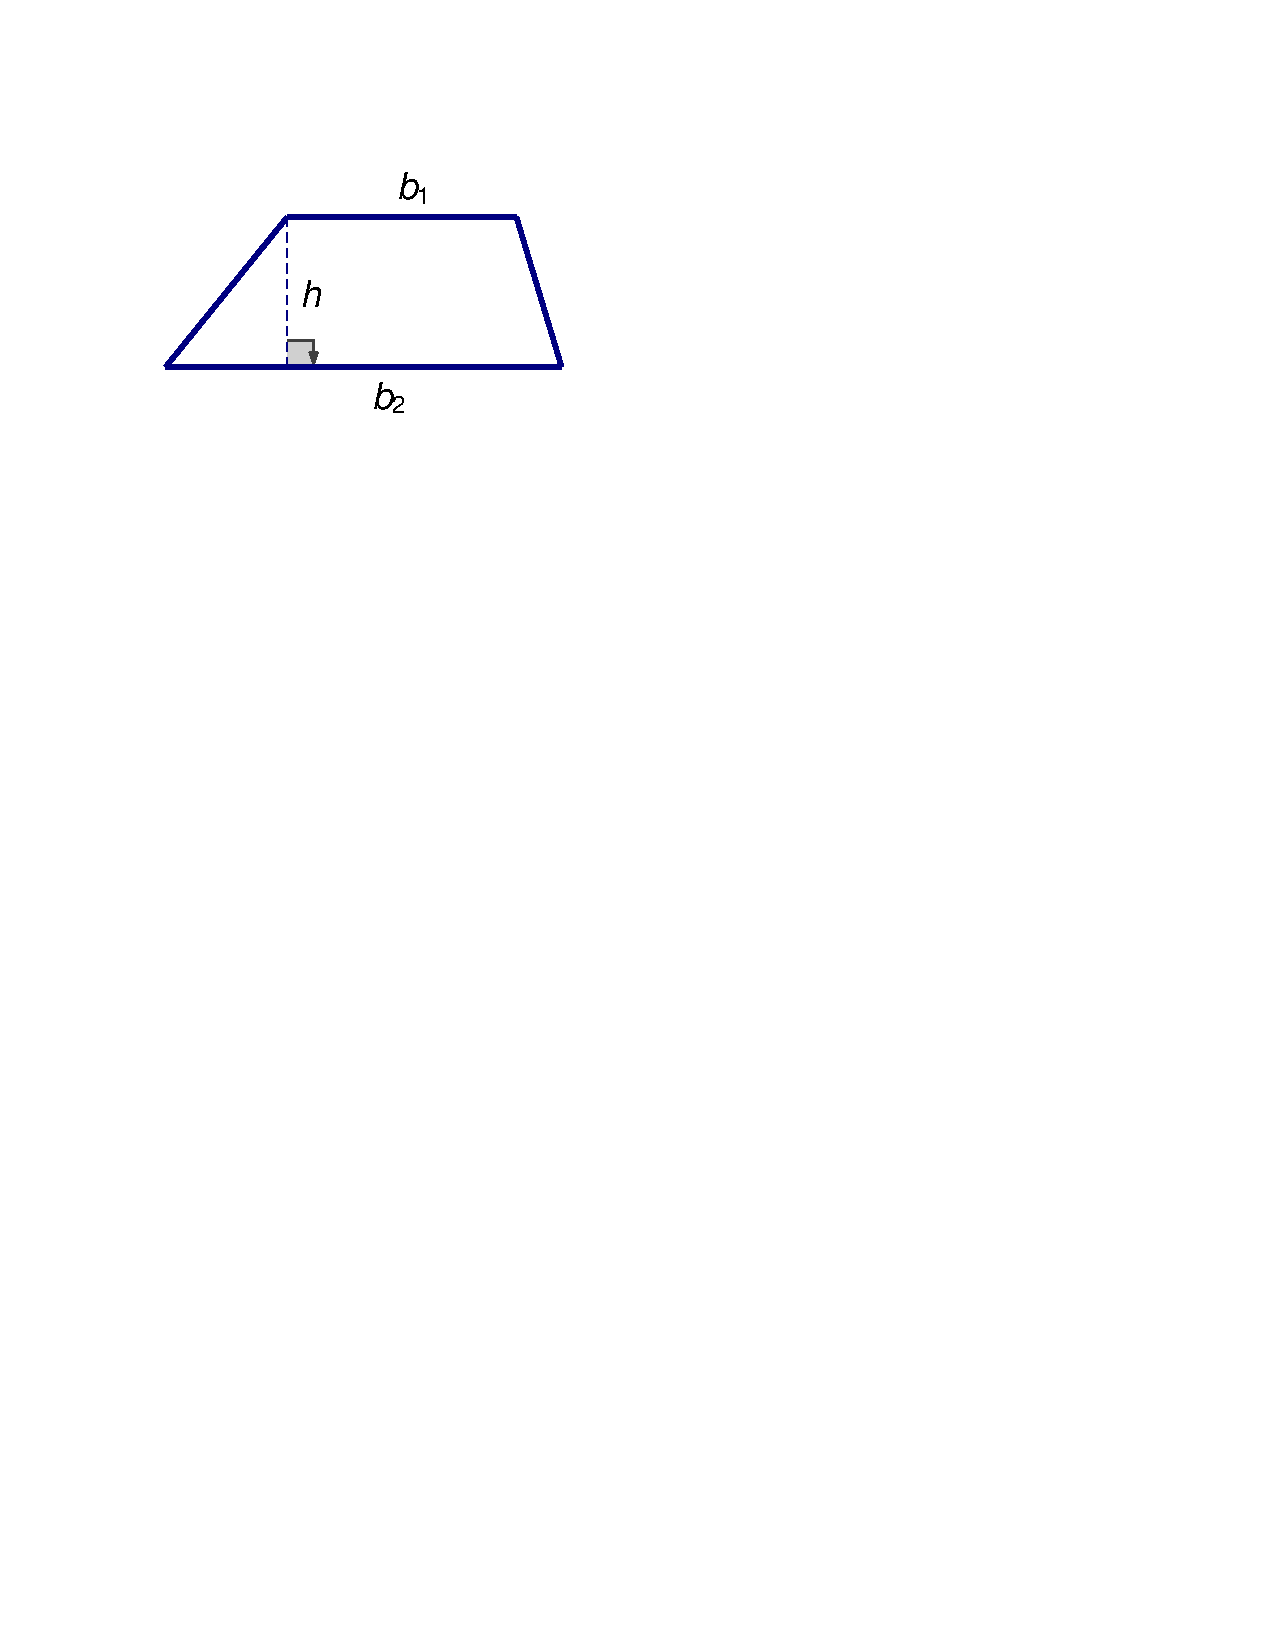
\includegraphics[scale=0.6]{trapezoid1.pdf}
\end{image}
Complete the table on the following page so that, in each row, the explanation, the geometric figure, and the algebraic formula together describe a way of computing the area.  For comparison purposes, each illustration should include a trapezoid congruent to the trapezoid above.   

All of the area formulas will, of course, be equivalent to one another as expressions.  But each way of expressing the area will make the most sense with figure and the explanation from the same row.  

\newpage


\newlength{\formulawidth}
\settowidth{\formulawidth}{$\frac{1}{2}b_2(x+h)-\frac{1}{2}b_1x$, with $\frac{x}{b_1}=\frac{x+h}{b_2}$}  
\resizebox{6in}{!}{ % use \textwidth instead of 6 in?
{\renewcommand{\arraystretch}{1.5}
\begin{tabular}{|>{\centering\arraybackslash}m{2.5cm}|>{\centering\arraybackslash}m{9.5cm}|c|}\hline
Explanation & Figure & Area Formula \\\hline

Rectangle with width that is the average of the bases. & 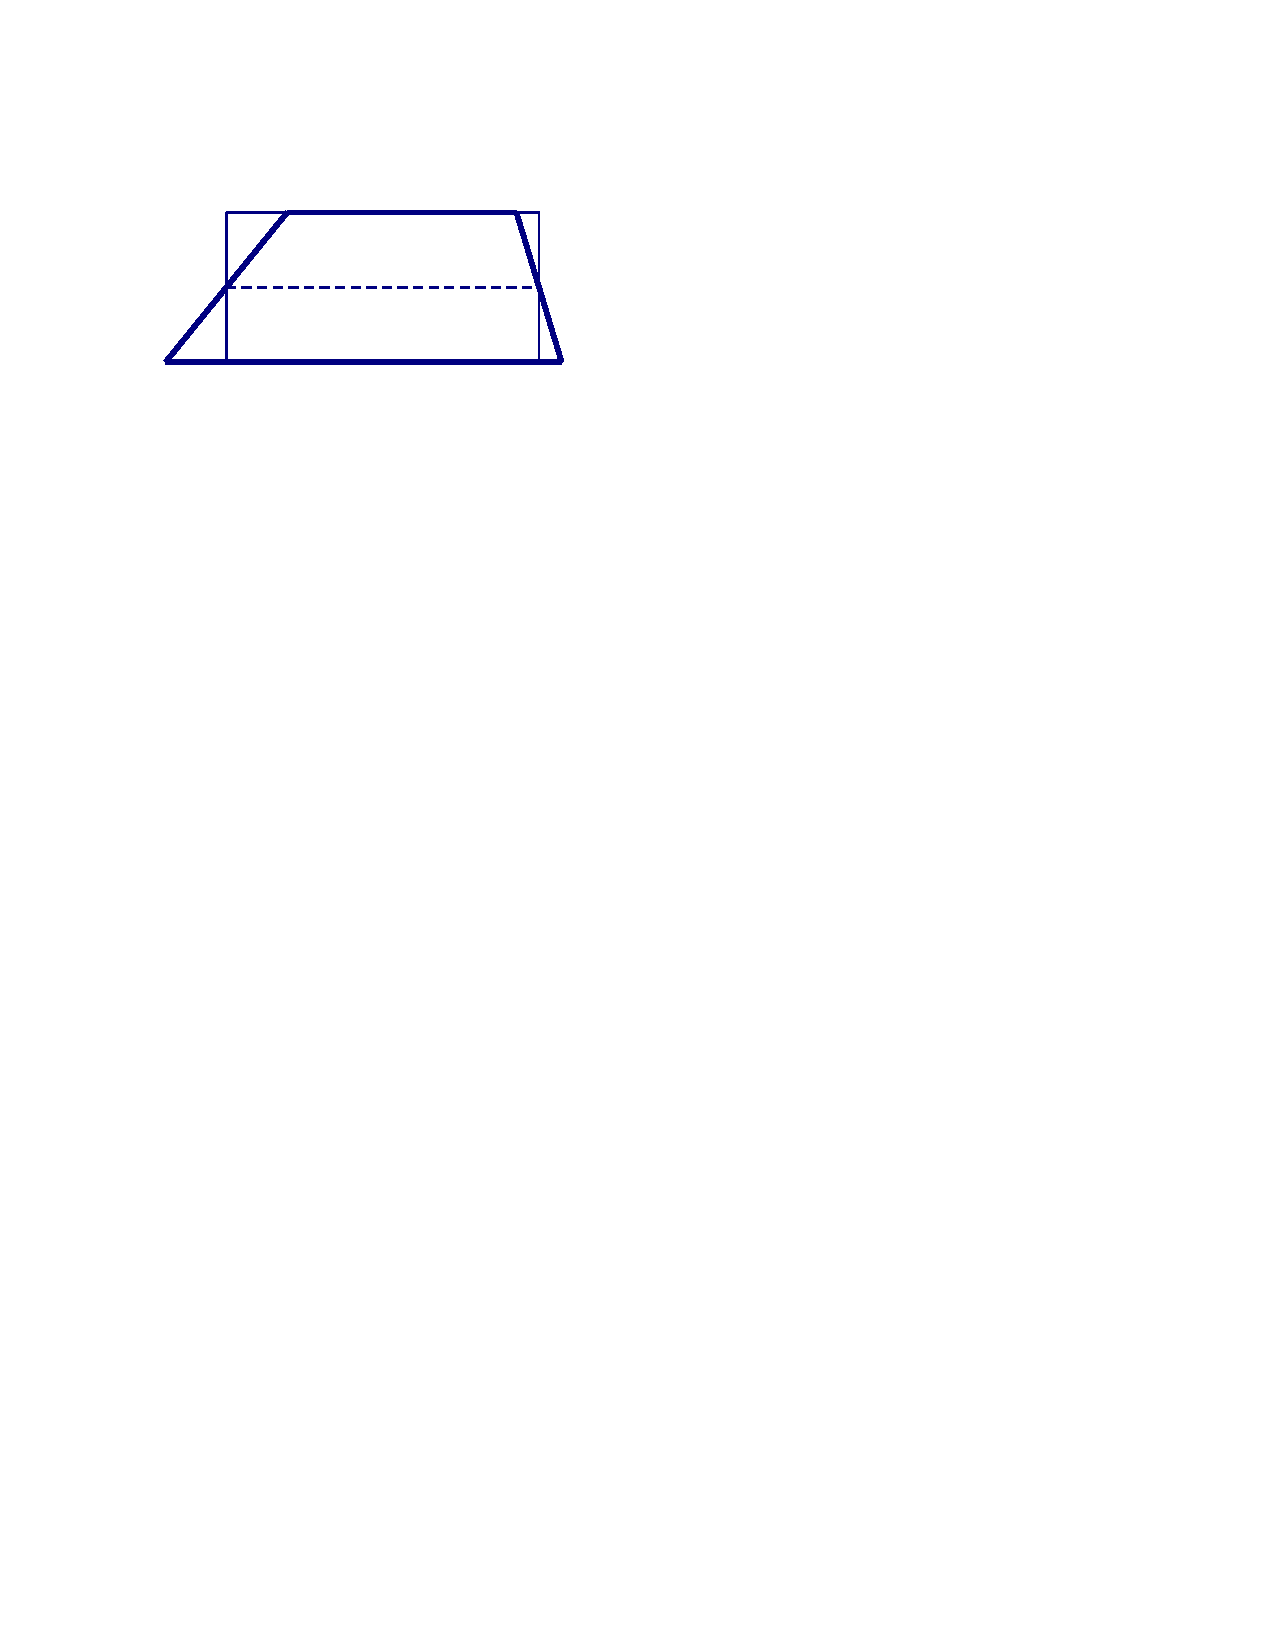
\includegraphics[scale=0.7]{trapezoid2.pdf} & $\left(\frac{b_1+b_2}{2}\right)h$ \\ \hline
                              & 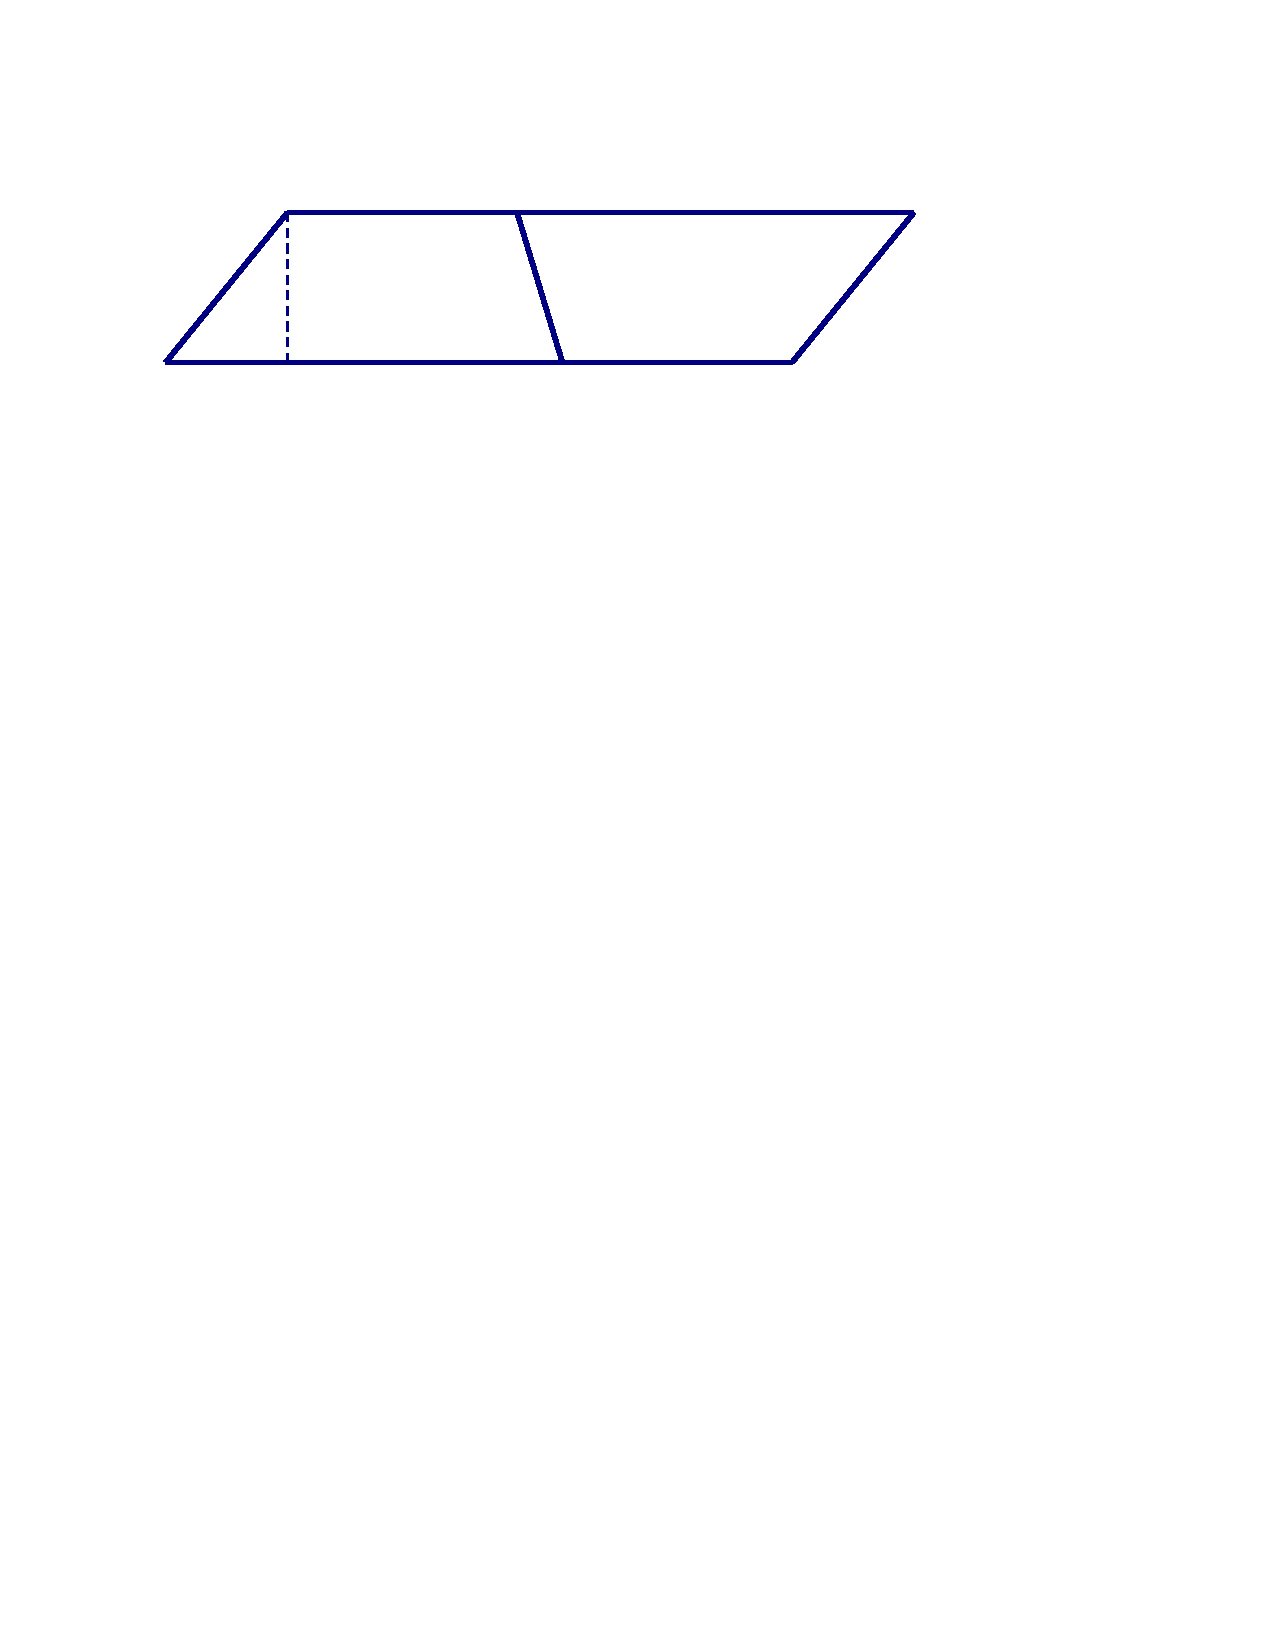
\includegraphics[scale=0.7]{trapezoid3.pdf} &                      \\ \hline
Two triangles with the same height and different bases. &                 & \\ \hline
 & & \\ 
\bigskip                              &  & $(b_1+b_2)\frac{h}{2}$ \\ 
 & & \\ \hline
          & 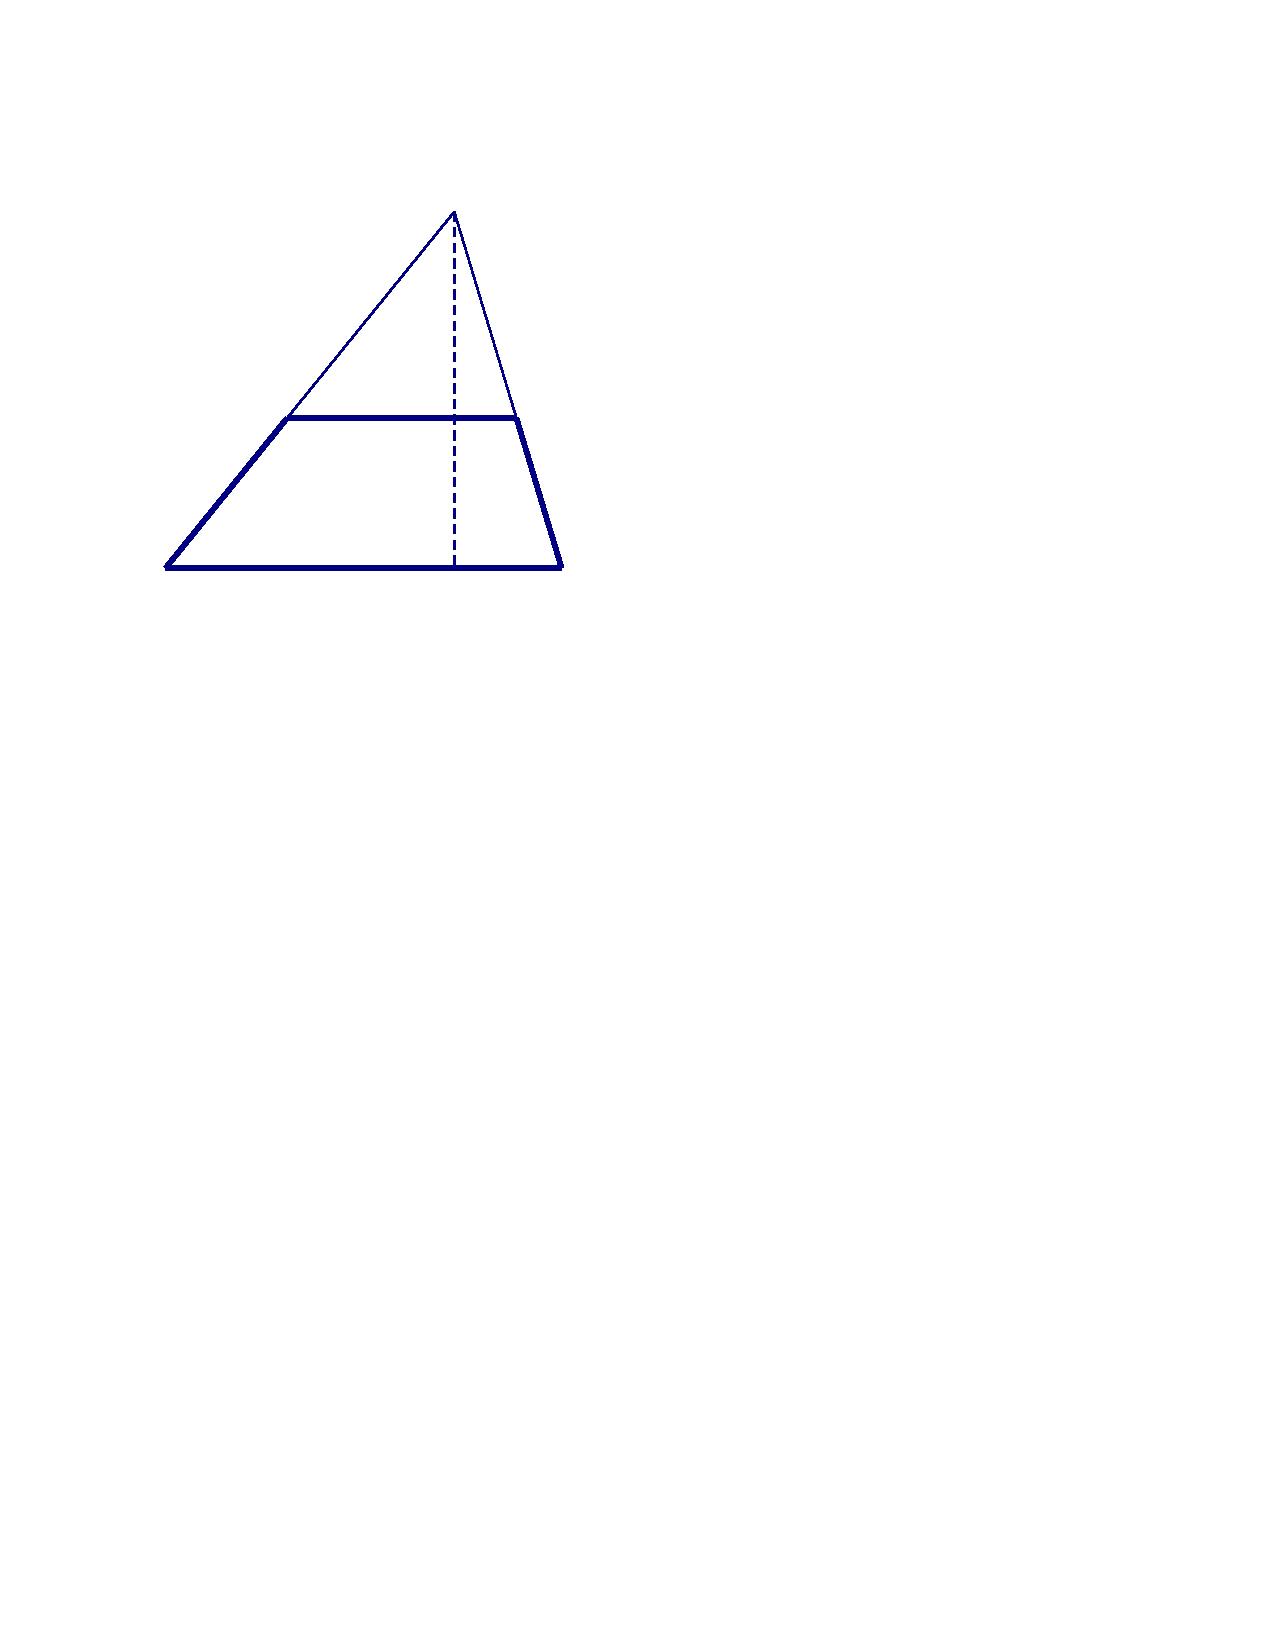
\includegraphics[scale=0.7]{trapezoid6.pdf}&  \hspace{\formulawidth} \\ \hline
\end{tabular}}
}
\end{problem}
%
%   Answers  
%
\newpage
\begin{teachingnote}
Answers:

\resizebox{\textwidth}{!}{
{\renewcommand{\arraystretch}{1.5}
\begin{tabular}{|>{\centering\arraybackslash}m{2.5cm}|>{\centering\arraybackslash}m{9.5cm}|c|}\hline
Explanation & Figure & Area Formula \\\hline

Rectangle with width that is the average of the bases. & 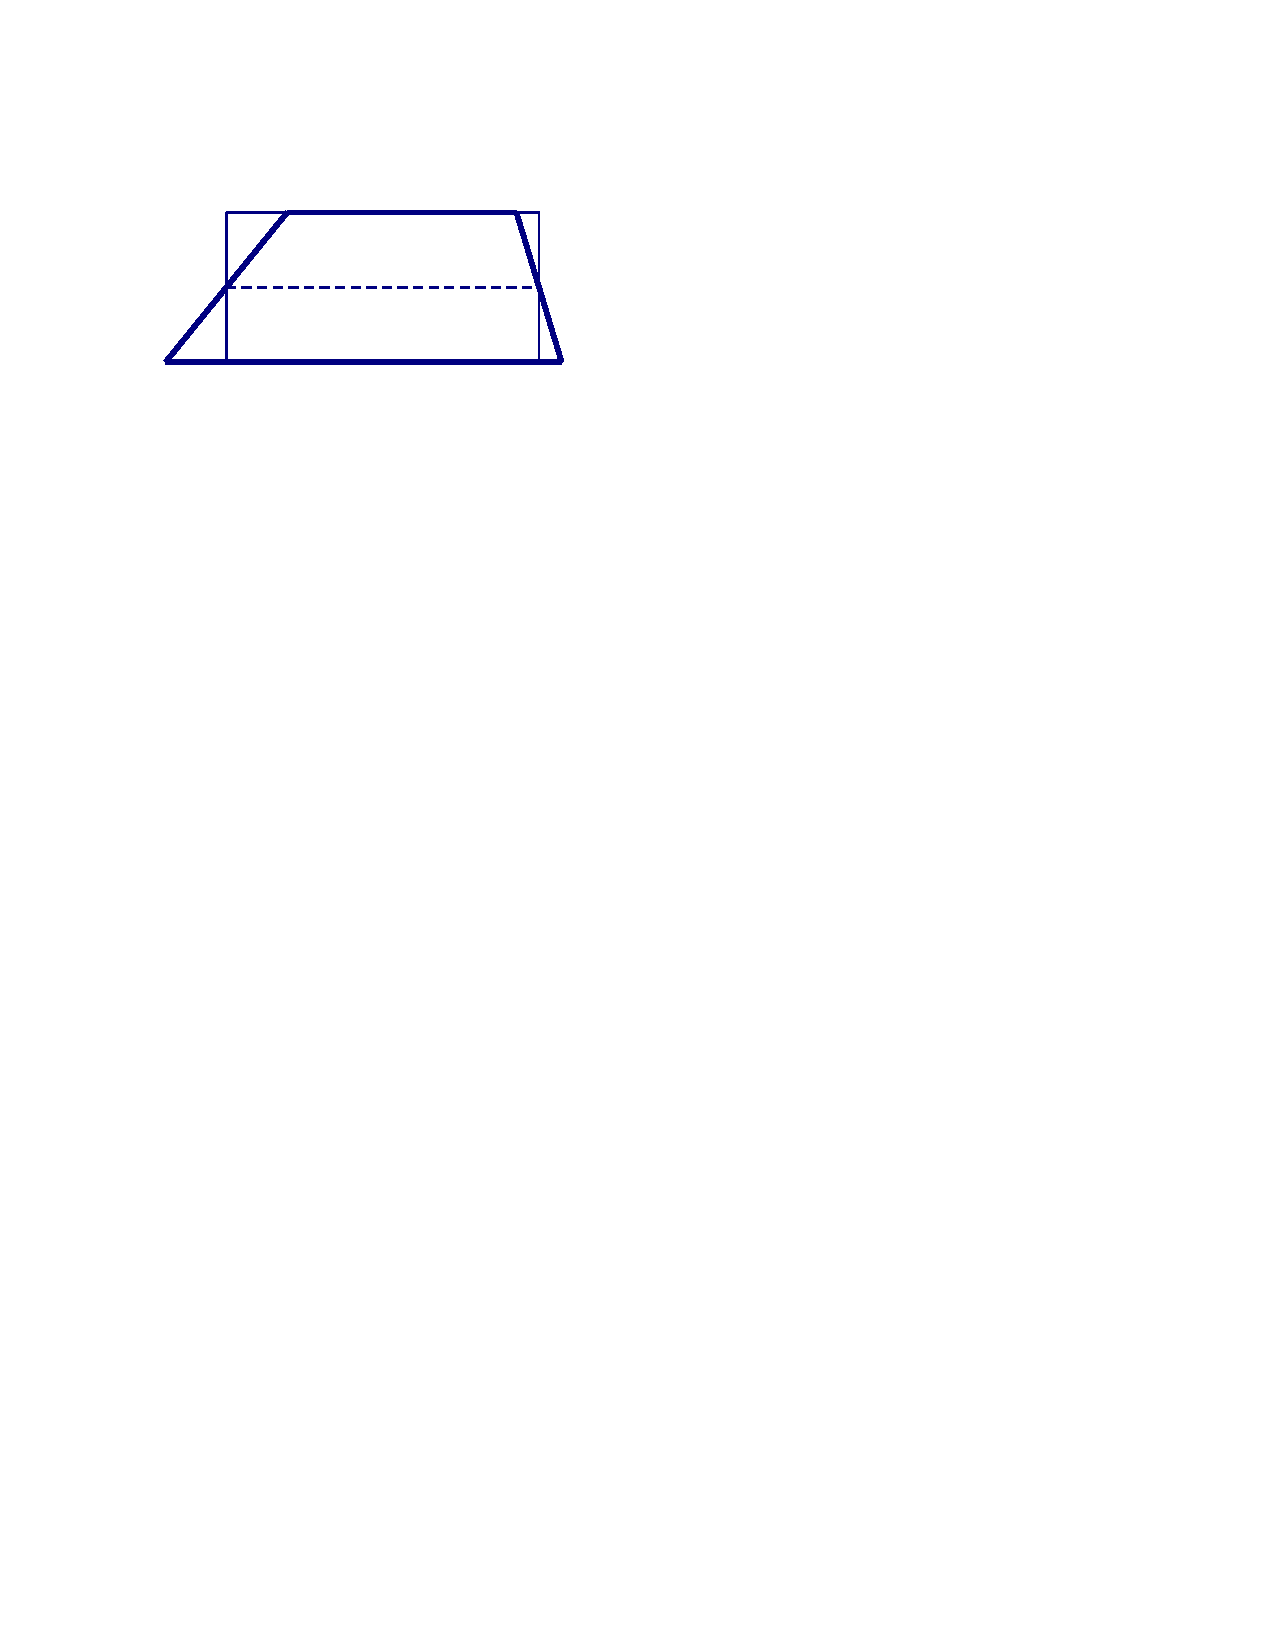
\includegraphics[scale=0.7]{trapezoid2.pdf} & $\left(\frac{b_1+b_2}{2}\right)h$ \\ \hline
Half of a large parallelogram. & 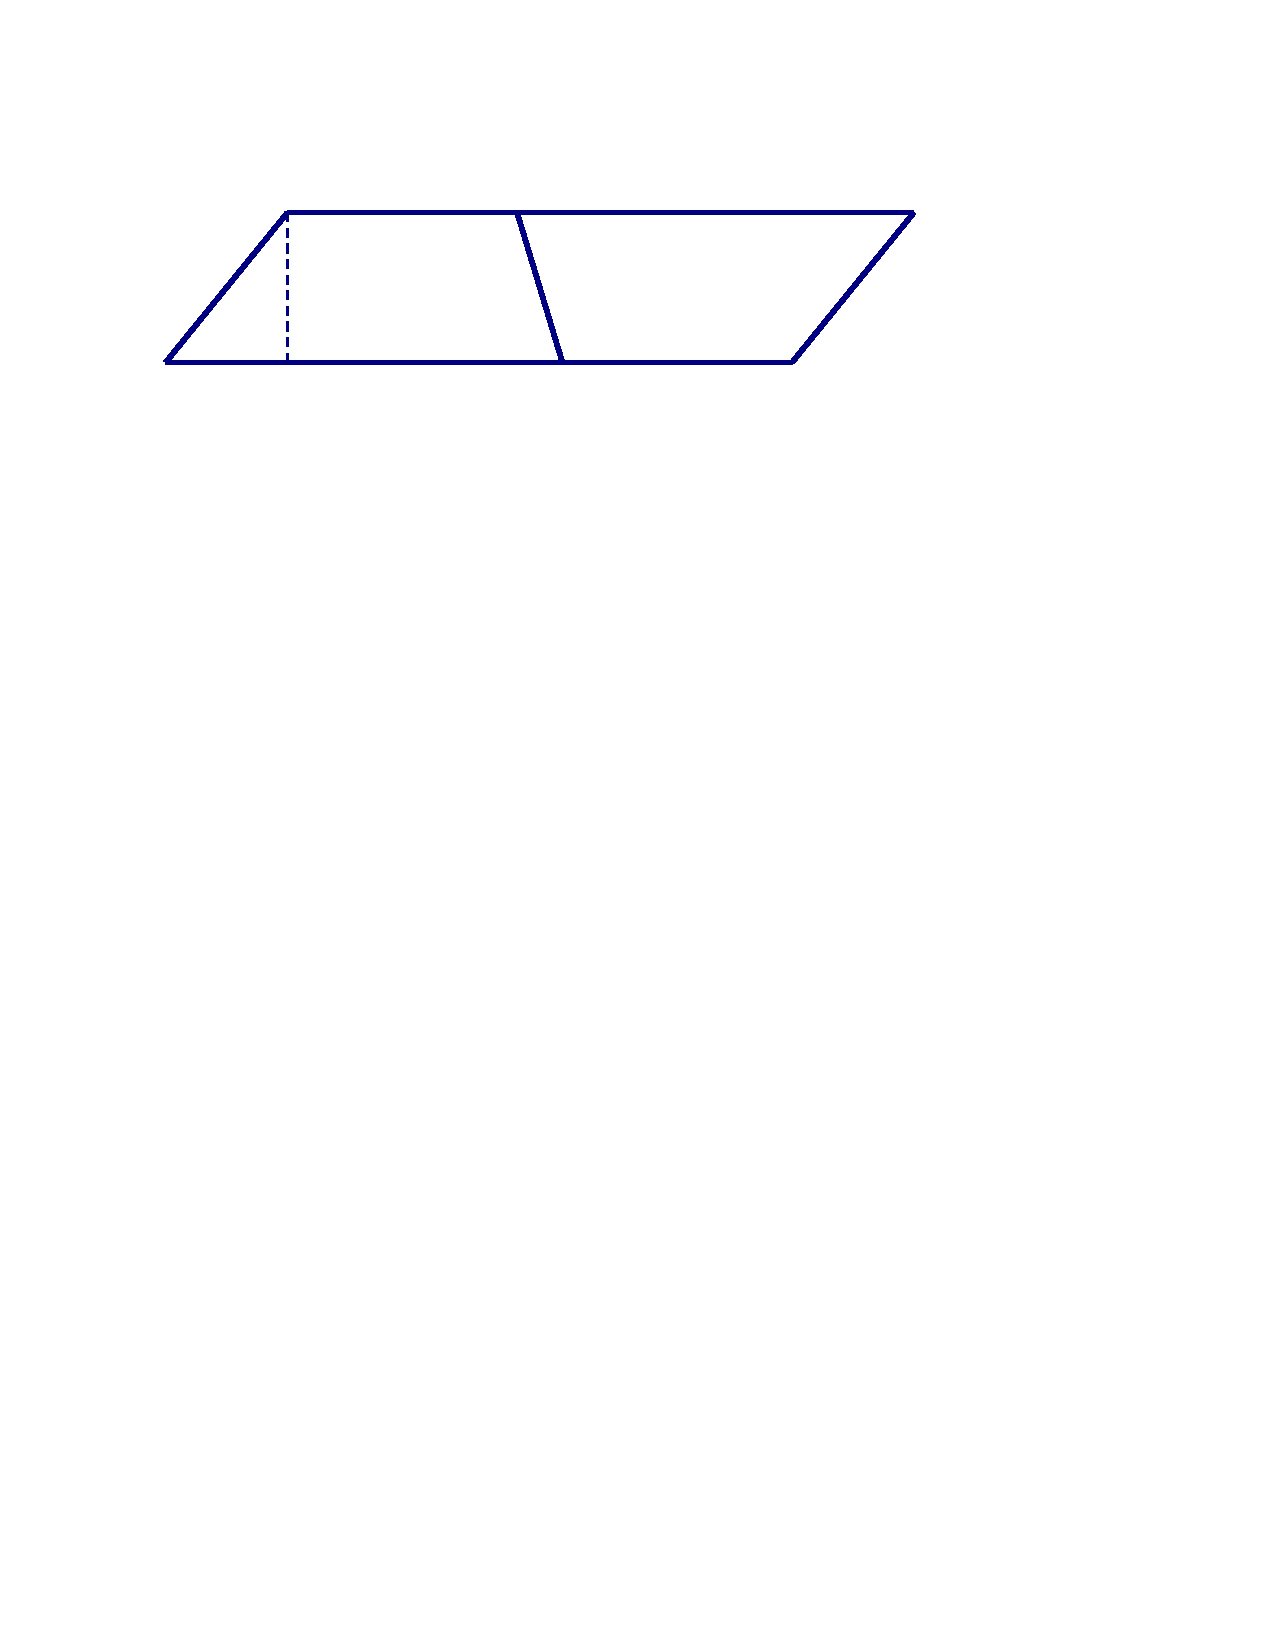
\includegraphics[scale=0.7]{trapezoid3.pdf} & $\frac{1}{2}(b_1+b_2)h$ \\ \hline
Two triangles with the same height and different bases. & 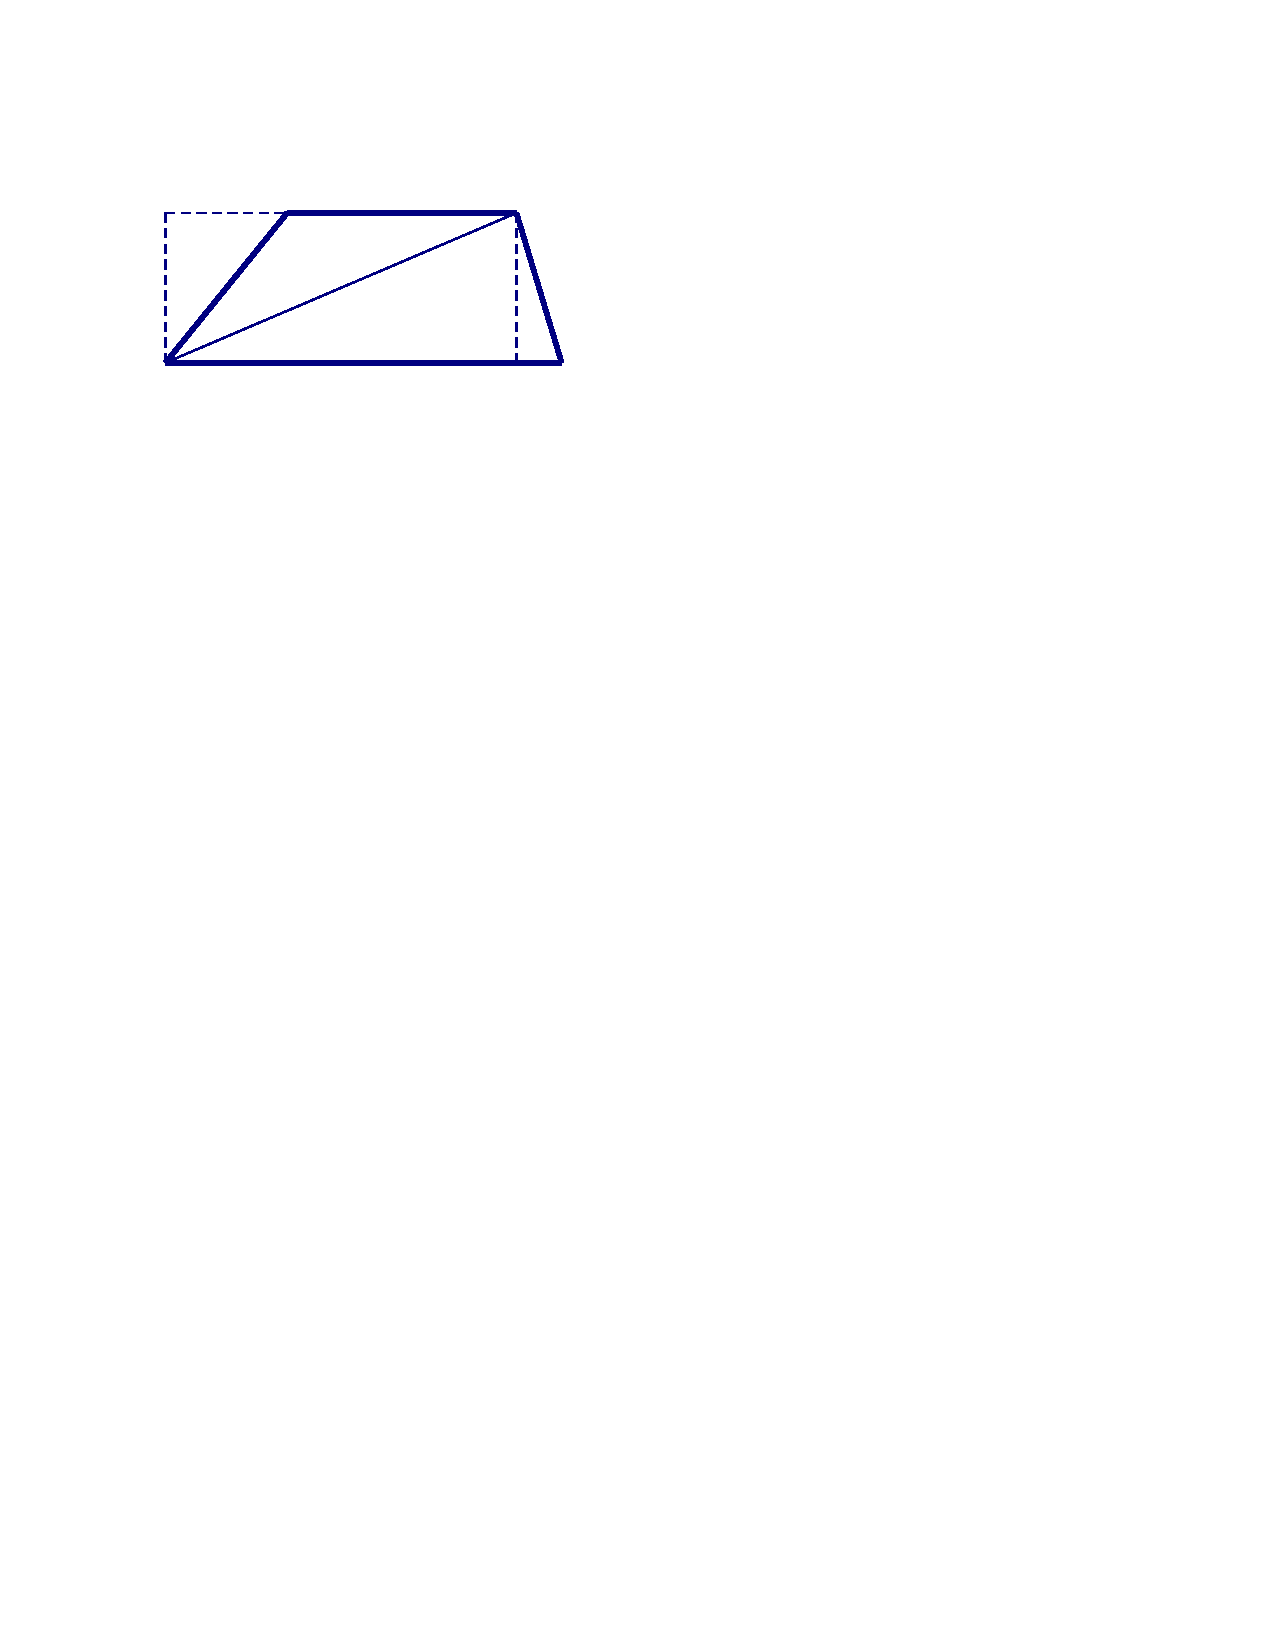
\includegraphics[scale=0.7]{trapezoid4.pdf} & $\frac{1}{2}b_1h + \frac{1}{2}b_2h$ \\ \hline
A parallelogram with half the height. & 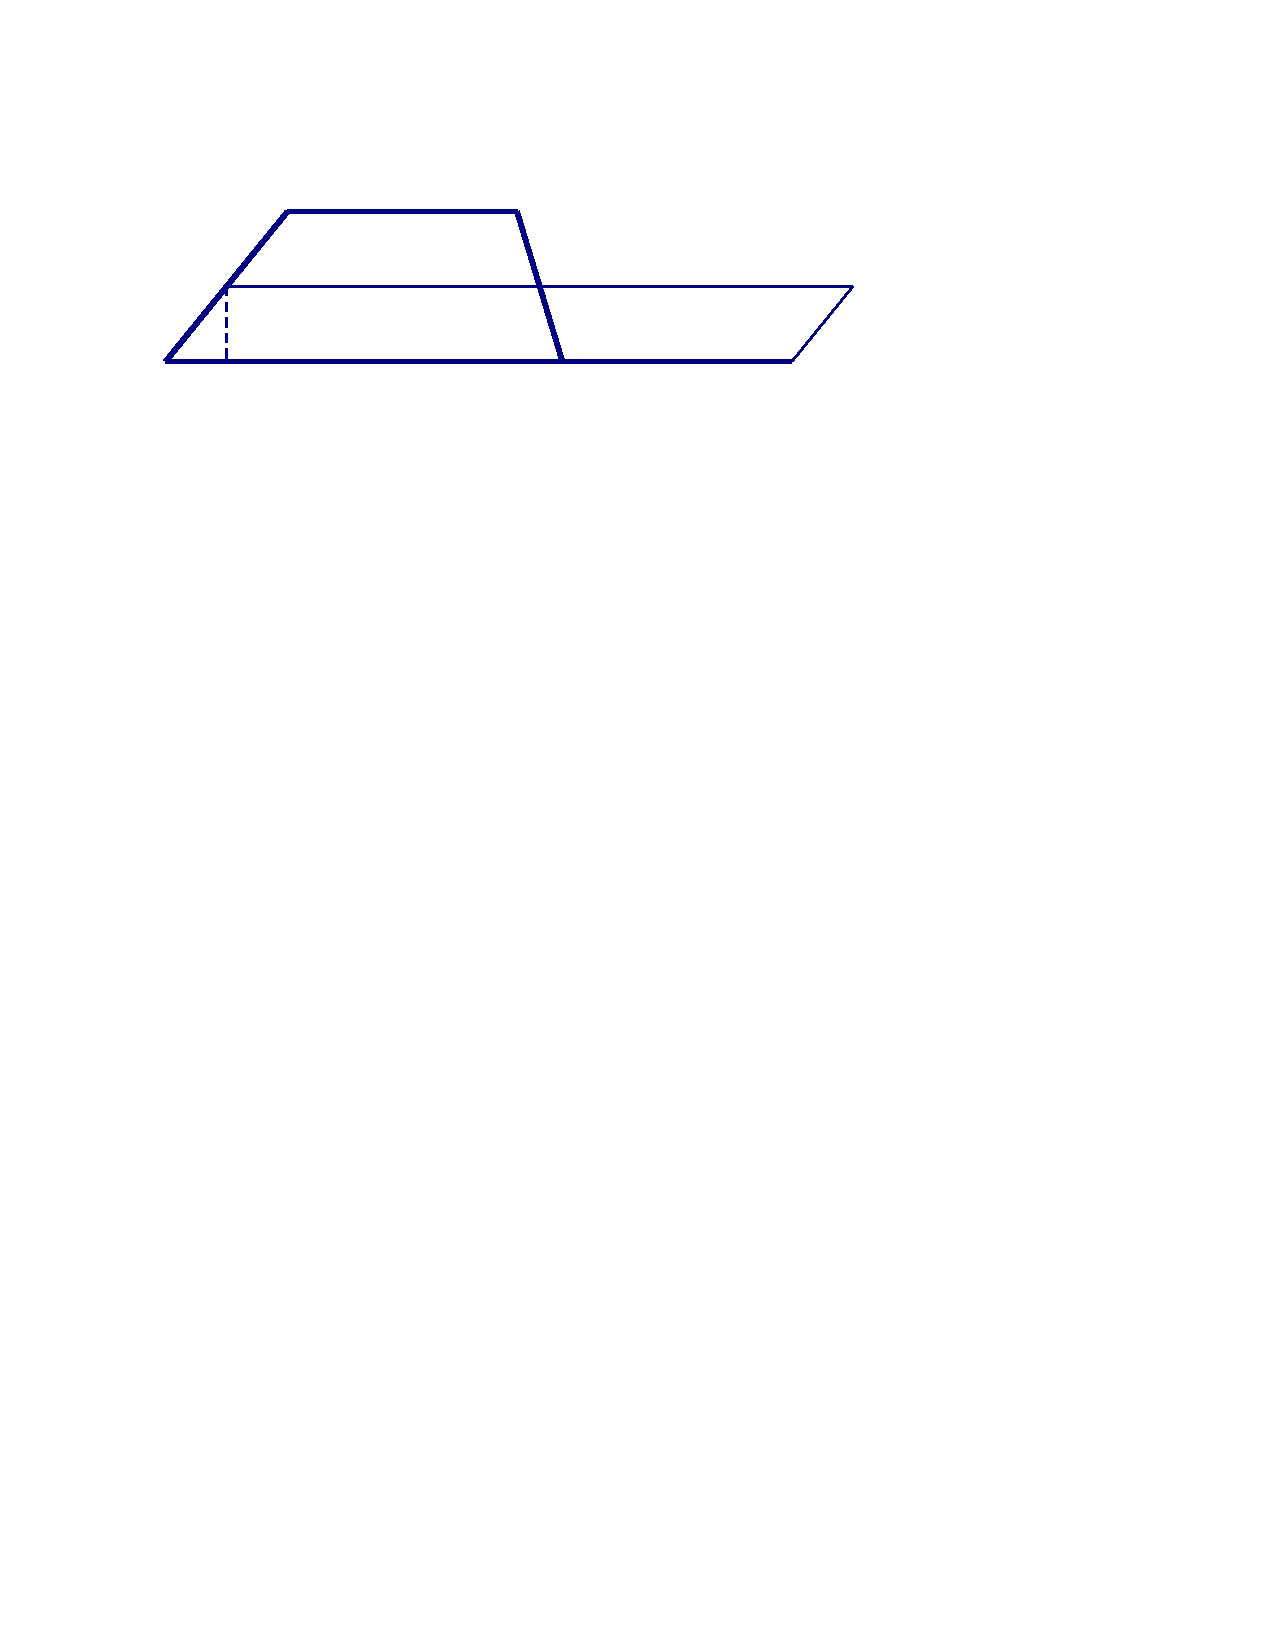
\includegraphics[scale=0.7]{trapezoid5.pdf} & $(b_1+b_2)\frac{h}{2}$ \\ \hline
Difference between two triangles, with $x$ as height of small triangle. 
          & 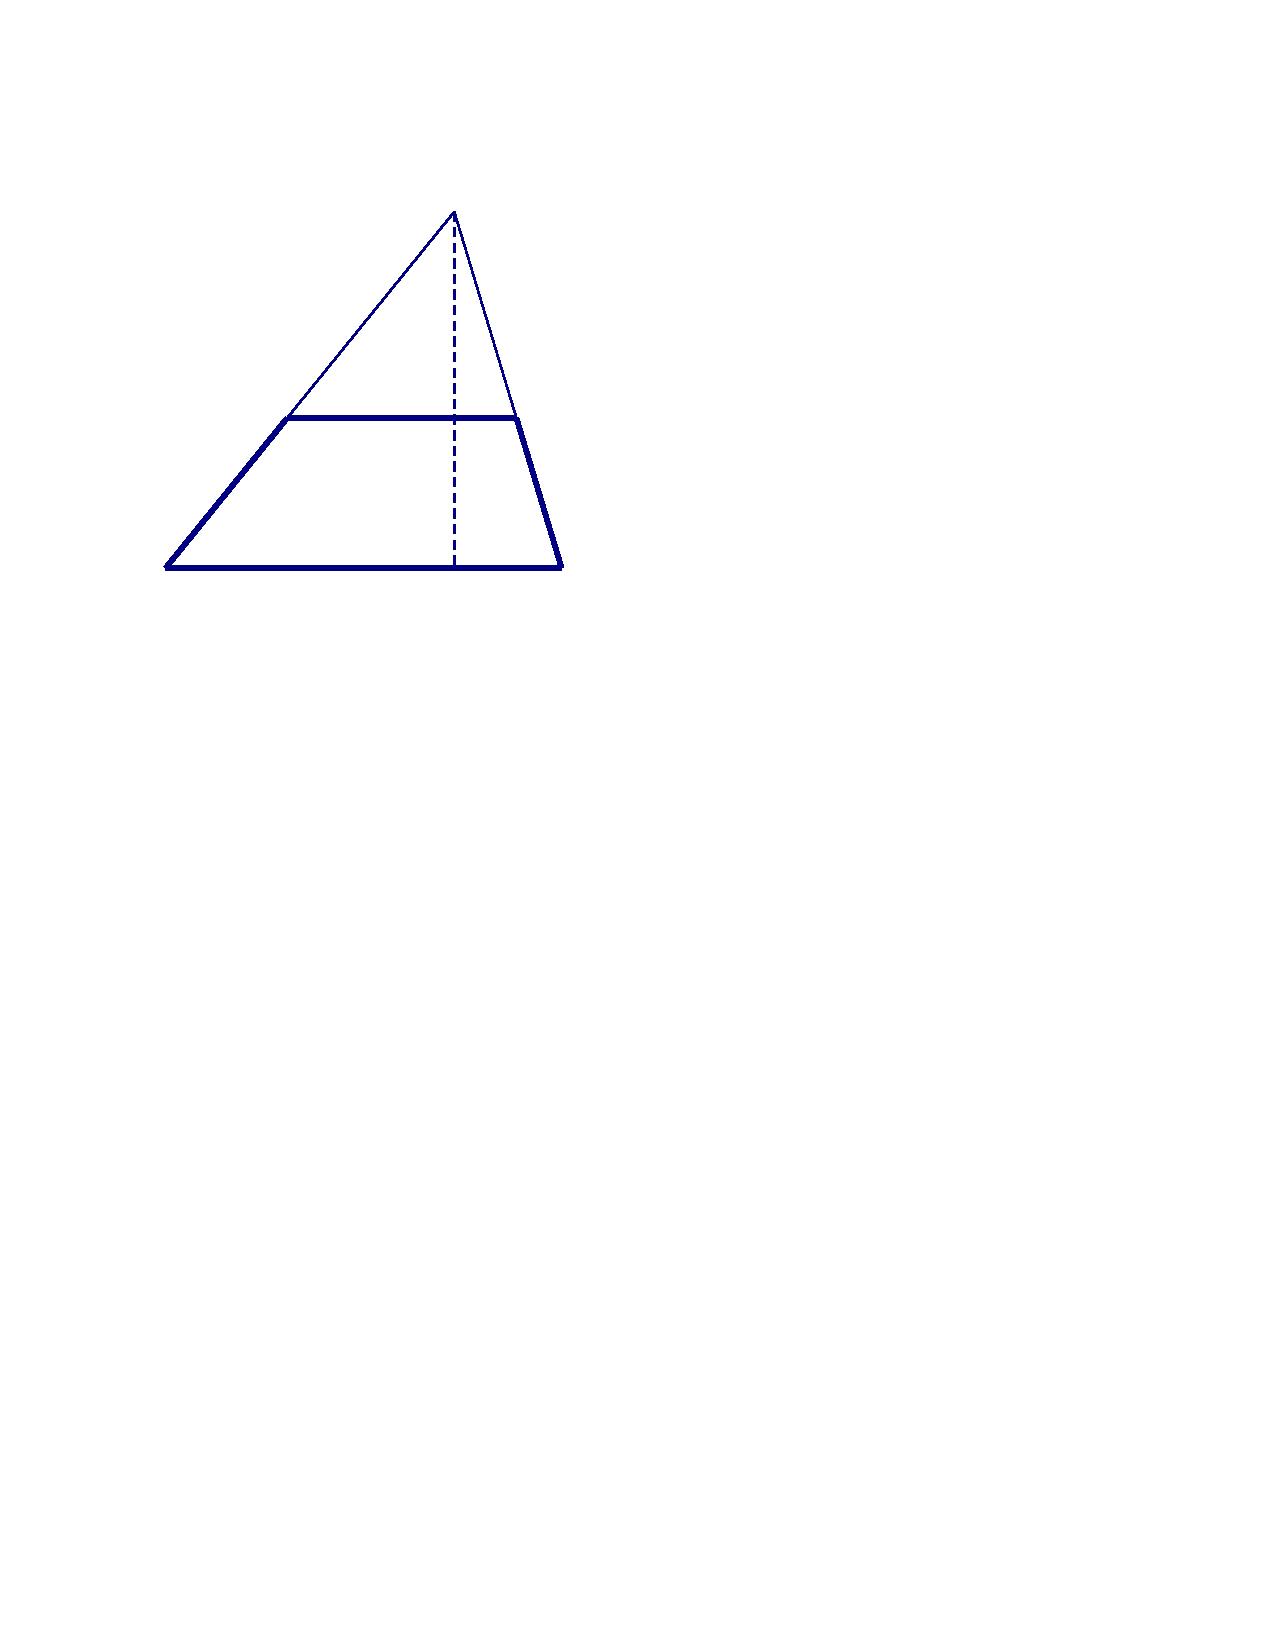
\includegraphics[scale=0.7]{trapezoid6.pdf} &  $\frac{1}{2}b_2(x+h)-\frac{1}{2}b_1x$, with $\frac{x}{b_1}=\frac{x+h}{b_2}$ \\ \hline
\end{tabular}}
}
\end{teachingnote}

\end{document}


% Constructions
%\documentclass[handout]{ximera}
\documentclass{ximera}

\usepackage{gensymb}
\usepackage{tabularx}
\usepackage{mdframed}
\usepackage{pdfpages}
%\usepackage{chngcntr}

\let\problem\relax
\let\endproblem\relax

\newcommand{\property}[2]{#1#2}




\newtheoremstyle{SlantTheorem}{\topsep}{\fill}%%% space between body and thm
 {\slshape}                      %%% Thm body font
 {}                              %%% Indent amount (empty = no indent)
 {\bfseries\sffamily}            %%% Thm head font
 {}                              %%% Punctuation after thm head
 {3ex}                           %%% Space after thm head
 {\thmname{#1}\thmnumber{ #2}\thmnote{ \bfseries(#3)}} %%% Thm head spec
\theoremstyle{SlantTheorem}
\newtheorem{problem}{Problem}[]

%\counterwithin*{problem}{section}



%%%%%%%%%%%%%%%%%%%%%%%%%%%%Jenny's code%%%%%%%%%%%%%%%%%%%%

%%% Solution environment
%\newenvironment{solution}{
%\ifhandout\setbox0\vbox\bgroup\else
%\begin{trivlist}\item[\hskip \labelsep\small\itshape\bfseries Solution\hspace{2ex}]
%\par\noindent\upshape\small
%\fi}
%{\ifhandout\egroup\else
%\end{trivlist}
%\fi}
%
%
%%% instructorIntro environment
%\ifhandout
%\newenvironment{instructorIntro}[1][false]%
%{%
%\def\givenatend{\boolean{#1}}\ifthenelse{\boolean{#1}}{\begin{trivlist}\item}{\setbox0\vbox\bgroup}{}
%}
%{%
%\ifthenelse{\givenatend}{\end{trivlist}}{\egroup}{}
%}
%\else
%\newenvironment{instructorIntro}[1][false]%
%{%
%  \ifthenelse{\boolean{#1}}{\begin{trivlist}\item[\hskip \labelsep\bfseries Instructor Notes:\hspace{2ex}]}
%{\begin{trivlist}\item[\hskip \labelsep\bfseries Instructor Notes:\hspace{2ex}]}
%{}
%}
%% %% line at the bottom} 
%{\end{trivlist}\par\addvspace{.5ex}\nobreak\noindent\hung} 
%\fi
%
%


\let\instructorNotes\relax
\let\endinstructorNotes\relax
%%% instructorNotes environment
\ifhandout
\newenvironment{instructorNotes}[1][false]%
{%
\def\givenatend{\boolean{#1}}\ifthenelse{\boolean{#1}}{\begin{trivlist}\item}{\setbox0\vbox\bgroup}{}
}
{%
\ifthenelse{\givenatend}{\end{trivlist}}{\egroup}{}
}
\else
\newenvironment{instructorNotes}[1][false]%
{%
  \ifthenelse{\boolean{#1}}{\begin{trivlist}\item[\hskip \labelsep\bfseries {\Large Instructor Notes: \\} \hspace{\textwidth} ]}
{\begin{trivlist}\item[\hskip \labelsep\bfseries {\Large Instructor Notes: \\} \hspace{\textwidth} ]}
{}
}
{\end{trivlist}}
\fi


%% Suggested Timing
\newcommand{\timing}[1]{{\bf Suggested Timing: \hspace{2ex}} #1}




\hypersetup{
    colorlinks=true,       % false: boxed links; true: colored links
    linkcolor=blue,          % color of internal links (change box color with linkbordercolor)
    citecolor=green,        % color of links to bibliography
    filecolor=magenta,      % color of file links
    urlcolor=cyan           % color of external links
}

\title{Triangle Investigation}
\author{Bart Snapp and Brad Findell}

\outcome{Learning outcome goes here.}

\begin{document}
\begin{abstract}
Abstract goes here.  
\end{abstract}
\maketitle

\begin{teachingnote}
Preactivity:  Do the first three of these at home.  The upshot is triangle congruence:  three measures are (often) enough.  

Some students will need to be reminded that, e.g., $B$ is vertex of $\angle ABC$.
\end{teachingnote}

\begin{problem}
Draw triangles satisfying the conditions given below.  You may use whatever tools you like (e.g., ruler, protractor, compass, sticks, tracing paper, or Geogebra).  

In each part, use reasoning to determine whether the information provided determines a unique $\triangle ABC$, more than one triangle, or no triangle.%\standard{7.G.2}   

Note:  To check to see if two triangles are the same, attempt to lay one directly on top of the other.  
\fixnote{Cite CCSS 7.G.2.}
\begin{enumerate}

\item $AB = 4$ and $BC = 5$
\item $m\angle CAB = 25^\circ$, $m\angle ABC = 75^\circ$, $m\angle BCA = 80^\circ$
\item $m\angle CAB = 25^\circ$, $m\angle ABC = 65^\circ$, $m\angle BCA = 80^\circ$
\item $AB = 4$, $m\angle BAC = 30^\circ$, $m\angle ABC = 45^\circ$
\item $AB = 4$, $BC = 5$, $m\angle ABC = 60^\circ$
\item $BC = 7$, $CA = 8$, $AB = 9$
\item $BC = 4$, $CA = 8$, $AB = 3$
\item $m\angle ABC = 45^\circ$, $BC = 8$, $CA = 12$
\item $m\angle ABC = 30^\circ$, $BC = 10$, $CA = 7$
\item $m\angle ABC = 60^\circ$, $BC = 10$, $CA = 3$

\end{enumerate}

\end{problem}

\end{document}

%\documentclass[handout]{ximera}
\documentclass[nooutcomes]{ximera}

\usepackage{gensymb}
\usepackage{tabularx}
\usepackage{mdframed}
\usepackage{pdfpages}
%\usepackage{chngcntr}

\let\problem\relax
\let\endproblem\relax

\newcommand{\property}[2]{#1#2}




\newtheoremstyle{SlantTheorem}{\topsep}{\fill}%%% space between body and thm
 {\slshape}                      %%% Thm body font
 {}                              %%% Indent amount (empty = no indent)
 {\bfseries\sffamily}            %%% Thm head font
 {}                              %%% Punctuation after thm head
 {3ex}                           %%% Space after thm head
 {\thmname{#1}\thmnumber{ #2}\thmnote{ \bfseries(#3)}} %%% Thm head spec
\theoremstyle{SlantTheorem}
\newtheorem{problem}{Problem}[]

%\counterwithin*{problem}{section}



%%%%%%%%%%%%%%%%%%%%%%%%%%%%Jenny's code%%%%%%%%%%%%%%%%%%%%

%%% Solution environment
%\newenvironment{solution}{
%\ifhandout\setbox0\vbox\bgroup\else
%\begin{trivlist}\item[\hskip \labelsep\small\itshape\bfseries Solution\hspace{2ex}]
%\par\noindent\upshape\small
%\fi}
%{\ifhandout\egroup\else
%\end{trivlist}
%\fi}
%
%
%%% instructorIntro environment
%\ifhandout
%\newenvironment{instructorIntro}[1][false]%
%{%
%\def\givenatend{\boolean{#1}}\ifthenelse{\boolean{#1}}{\begin{trivlist}\item}{\setbox0\vbox\bgroup}{}
%}
%{%
%\ifthenelse{\givenatend}{\end{trivlist}}{\egroup}{}
%}
%\else
%\newenvironment{instructorIntro}[1][false]%
%{%
%  \ifthenelse{\boolean{#1}}{\begin{trivlist}\item[\hskip \labelsep\bfseries Instructor Notes:\hspace{2ex}]}
%{\begin{trivlist}\item[\hskip \labelsep\bfseries Instructor Notes:\hspace{2ex}]}
%{}
%}
%% %% line at the bottom} 
%{\end{trivlist}\par\addvspace{.5ex}\nobreak\noindent\hung} 
%\fi
%
%


\let\instructorNotes\relax
\let\endinstructorNotes\relax
%%% instructorNotes environment
\ifhandout
\newenvironment{instructorNotes}[1][false]%
{%
\def\givenatend{\boolean{#1}}\ifthenelse{\boolean{#1}}{\begin{trivlist}\item}{\setbox0\vbox\bgroup}{}
}
{%
\ifthenelse{\givenatend}{\end{trivlist}}{\egroup}{}
}
\else
\newenvironment{instructorNotes}[1][false]%
{%
  \ifthenelse{\boolean{#1}}{\begin{trivlist}\item[\hskip \labelsep\bfseries {\Large Instructor Notes: \\} \hspace{\textwidth} ]}
{\begin{trivlist}\item[\hskip \labelsep\bfseries {\Large Instructor Notes: \\} \hspace{\textwidth} ]}
{}
}
{\end{trivlist}}
\fi


%% Suggested Timing
\newcommand{\timing}[1]{{\bf Suggested Timing: \hspace{2ex}} #1}




\hypersetup{
    colorlinks=true,       % false: boxed links; true: colored links
    linkcolor=blue,          % color of internal links (change box color with linkbordercolor)
    citecolor=green,        % color of links to bibliography
    filecolor=magenta,      % color of file links
    urlcolor=cyan           % color of external links
}

\title{UnMessUpable Figures}
\author{Bart Snapp and Brad Findell}

\outcome{Learning outcome goes here.}

\begin{document}
\begin{abstract}
  We model Euclidean constructions in dynamic geometry software.
\end{abstract}
\maketitle

\begin{teachingnote}
This serves as an introduction to dynamic geometry software.  

If Euclid the Game is available, then use its Tutorial and levels 1 through 12 instead of this activity.  Note:  Most bugs in Euclid the Game are fixed by refreshing the page. 

The last two problems are optional.
\end{teachingnote}

 
Suppose we draw or a construct a geometric figure (e.g., a square or an isosceles triangle) with pencil, paper, compass, and straightedge.  If we want to compare to another example of that type of figure, we need to begin again from scratch.  With dynamic geometry software (e.g., \textsl{Geogebra}, \textsl{Geometer's Sketchpad}, or \textsl{Cabri}), we can alter the original figure by ``dragging'' vertices and segments to create many other examples.  For this to work properly, we want to \emph{construct} the figure rather than merely \emph{draw} it, so that a square, for example, remains a square even if we move its vertices.  Some folks call such figures ``UnMessUpable.'' 

\vspace{0.1in}
\begin{center}
\textbf{Rules of Engagement:}
\end{center}
\begin{itemize}
\itemsep0em
\item Before you begin, explore the menus and toolbars to see what the software provides.  
\item You may use tools that function as a compass or straight-edge would.  
\item You may use special tools (e.g., perpendicular bisector) that accomplish multistep     
compass-and-straightedge constructions in a single step.
\item Do not use tools for transformations (e.g., translations, reflections, or rotations).
\item Do not use tools that construct objects from measurements.  
\end{itemize}

\begin{center}
\textbf{Begin each problem in a new sketch.}
\end{center}

\begin{problem}
Construct a segment between two points.  Then construct an equilateral triangle with that segment as one of its sides.  Be sure that the triangle remains equilateral when you drag its vertices.   (Note:  Do not use a ``regular polygon'' tool.)
\end{problem}

\begin{problem}
Construct a segment between two points.  Then construct a square with that segment as one of its sides.  Be sure that it remains a square when you drag its vertices.  (Note:  Do not use a ``regular polygon'' tool.)
\end{problem}

\begin{problem}
Construct an UnMessUpable parallelogram.  (Hint:  Think about the definition.)  
\end{problem}

\begin{problem}
Construct a rectangle that, through dragging, can be long and thin, short and fat, or anything in between, but that is always a rectangle.
\end{problem}

\begin{problem}
\emph{Copy a segment.}  Construct a segment and a line.  Then copy the segment onto the line.  Hide the line so that the segment alone is clear.  Then drag the vertices that determine the initial segment to show that the copy is always congruent to it.  
\end{problem}

\begin{problem}
\emph{Copy an angle.}  Using the ray tool, construct an angle and a separate ray.  Then copy the angle onto the other ray.  Drag the vertices that determine the first angle to show that the copy is always congruent to it.  
\end{problem}

\begin{problem}
Construct a capital H so that the midline is always the perpendicular bisector of both sides.  
\end{problem}

\begin{problem}
Construct a quadrilateral so that one pair of opposite sides is always congruent.  
\end{problem}

\end{document}

%\documentclass[handout]{ximera}
\documentclass{ximera}

\usepackage{gensymb}
\usepackage{tabularx}
\usepackage{mdframed}
\usepackage{pdfpages}
%\usepackage{chngcntr}

\let\problem\relax
\let\endproblem\relax

\newcommand{\property}[2]{#1#2}




\newtheoremstyle{SlantTheorem}{\topsep}{\fill}%%% space between body and thm
 {\slshape}                      %%% Thm body font
 {}                              %%% Indent amount (empty = no indent)
 {\bfseries\sffamily}            %%% Thm head font
 {}                              %%% Punctuation after thm head
 {3ex}                           %%% Space after thm head
 {\thmname{#1}\thmnumber{ #2}\thmnote{ \bfseries(#3)}} %%% Thm head spec
\theoremstyle{SlantTheorem}
\newtheorem{problem}{Problem}[]

%\counterwithin*{problem}{section}



%%%%%%%%%%%%%%%%%%%%%%%%%%%%Jenny's code%%%%%%%%%%%%%%%%%%%%

%%% Solution environment
%\newenvironment{solution}{
%\ifhandout\setbox0\vbox\bgroup\else
%\begin{trivlist}\item[\hskip \labelsep\small\itshape\bfseries Solution\hspace{2ex}]
%\par\noindent\upshape\small
%\fi}
%{\ifhandout\egroup\else
%\end{trivlist}
%\fi}
%
%
%%% instructorIntro environment
%\ifhandout
%\newenvironment{instructorIntro}[1][false]%
%{%
%\def\givenatend{\boolean{#1}}\ifthenelse{\boolean{#1}}{\begin{trivlist}\item}{\setbox0\vbox\bgroup}{}
%}
%{%
%\ifthenelse{\givenatend}{\end{trivlist}}{\egroup}{}
%}
%\else
%\newenvironment{instructorIntro}[1][false]%
%{%
%  \ifthenelse{\boolean{#1}}{\begin{trivlist}\item[\hskip \labelsep\bfseries Instructor Notes:\hspace{2ex}]}
%{\begin{trivlist}\item[\hskip \labelsep\bfseries Instructor Notes:\hspace{2ex}]}
%{}
%}
%% %% line at the bottom} 
%{\end{trivlist}\par\addvspace{.5ex}\nobreak\noindent\hung} 
%\fi
%
%


\let\instructorNotes\relax
\let\endinstructorNotes\relax
%%% instructorNotes environment
\ifhandout
\newenvironment{instructorNotes}[1][false]%
{%
\def\givenatend{\boolean{#1}}\ifthenelse{\boolean{#1}}{\begin{trivlist}\item}{\setbox0\vbox\bgroup}{}
}
{%
\ifthenelse{\givenatend}{\end{trivlist}}{\egroup}{}
}
\else
\newenvironment{instructorNotes}[1][false]%
{%
  \ifthenelse{\boolean{#1}}{\begin{trivlist}\item[\hskip \labelsep\bfseries {\Large Instructor Notes: \\} \hspace{\textwidth} ]}
{\begin{trivlist}\item[\hskip \labelsep\bfseries {\Large Instructor Notes: \\} \hspace{\textwidth} ]}
{}
}
{\end{trivlist}}
\fi


%% Suggested Timing
\newcommand{\timing}[1]{{\bf Suggested Timing: \hspace{2ex}} #1}




\hypersetup{
    colorlinks=true,       % false: boxed links; true: colored links
    linkcolor=blue,          % color of internal links (change box color with linkbordercolor)
    citecolor=green,        % color of links to bibliography
    filecolor=magenta,      % color of file links
    urlcolor=cyan           % color of external links
}

\title{Triangle Centers}
\author{Bart Snapp and Brad Findell}

\outcome{Learning outcome goes here.}

\begin{document}
\begin{abstract}
Abstract goes here.  
\end{abstract}
\maketitle

\begin{teachingnote}
This exploration introduces perpendicular bisectors, angle bisectors, medians, and altitudes and the idea of concurrency.  

Use a Geogebra to demonstrate that two points determines a family of circles.  A third point (usually) specifies the circle.
\end{teachingnote}

In this activity, we use \textsl{Geogebra} to explore the basic lines, centers, and circles related to triangles.  

\begin{problem} Here are some easy questions to get the brain-juices flowing!
\begin{enumerate} 
\itemsep -3pt
\item Place two points randomly in the plane. Do you expect to be able to
draw a single line that connects them?
\item Place three points randomly in the plane. Do you expect to be able to
draw a single line that connects them?
\item Place two lines randomly in the plane. How many points do you expect
them to share?
\item Place three lines randomly in the plane. How many points do you expect
all three lines to share?
\item Place two points randomly in the plane. Will you always be
able to draw a circle containing these points?
\item Place three points randomly in the plane. Will you (almost!) always be
able to draw a circle containing these points? If no, why not? If yes,
how do you know?
\item Place four points randomly in the plane. Do you expect to be able to
draw a circle containing all four at once? Explain your reasoning.
\end{enumerate}
\end{problem}

\begin{definition}
Three (or more) distinct lines are said to be \textbf{concurrent} if they have a point in common.  
\end{definition}

\begin{problem} 
In \textsl{Geogebra}, draw a triangle. Now construct the perpendicular bisectors of
the sides.  Describe what you notice.  Does this work for every triangle?
\end{problem}

\begin{problem}
In a new \textsl{Geogebra} sketch, draw a triangle. Now bisect the angles.  Describe what you notice.  Does this work for every
triangle?
\end{problem}

\begin{problem}
In a new \textsl{Geogebra} sketch, draw a triangle. Now construct the lines containing the altitudes.  Describe what you notice.  
Does this work for every triangle?
\end{problem}

\begin{problem}
In a new \textsl{Geogebra} sketch, draw a triangle. Now construct the medians.  Describe what you notice.  Does this work for every triangle?
\end{problem}

\begin{problem}
The \textbf{circumcircle} of a triangle contains all three vertices of the triangle.  The center of the circumcircle is called the \textbf{circumcenter}.  Find the circumcenter on your sketch with the three perpendicular bisectors, and construct the circumcircle.  
\end{problem}

\begin{problem}
The \textbf{incircle} of a triangle is tangent to all three sides of the triangle.  The center of the incircle is called the \textbf{incenter}.  
Find the incenter on your sketch with three angle bisectors. Construct the incircle.  (Hint:  To find the radius of the incircle, you will need to find the distance from the incenter to one of the sides of the triangle.)  
\end{problem}

\begin{problem}
The other ``centers'' of a triangle are called the \textbf{centroid} and the \textbf{orthocenter}.  Make a thoughtful guess about how these correspond to the medians and the lines containing the altitudes.  
\end{problem}


\begin{problem}
Fill in the following handy chart summarizing what you found above. 
\[
\begin{tabular}{| l || c | c | c |}
\hline
  & Associated point? & \begin{minipage}{14ex}\minipad Always inside the triangle? \minipad\end{minipage} & Meaning? \\ \hline\hline 
\begin{minipage}{12ex}\minipad perpendicular \\ bisectors \minipad\end{minipage}  &\hspace{25mm} &\hspace{15mm}  & \hspace{100mm} \\ \hline
\begin{minipage}{12ex}\minipad angle \\ bisectors \minipad\end{minipage} & \rule[0mm]{0mm}{7mm}    &  & \\ \hline
\begin{minipage}{12ex}\minipad lines \\ containing altitudes \minipad\end{minipage} & \rule[0mm]{0mm}{7mm}    &  &  \\ \hline
\begin{minipage}{12ex}\minipad lines \\ containing the medians  \minipad\end{minipage} & \rule[0mm]{0mm}{7mm}   &  &   \\ \hline
\end{tabular}
\]
Be sure to put this in a safe place like in a safe, or under your bed.
\end{problem}
\end{document}

%\documentclass[handout]{ximera}
\documentclass[nooutcomes]{ximera}

\usepackage{gensymb}
\usepackage{tabularx}
\usepackage{mdframed}
\usepackage{pdfpages}
%\usepackage{chngcntr}

\let\problem\relax
\let\endproblem\relax

\newcommand{\property}[2]{#1#2}




\newtheoremstyle{SlantTheorem}{\topsep}{\fill}%%% space between body and thm
 {\slshape}                      %%% Thm body font
 {}                              %%% Indent amount (empty = no indent)
 {\bfseries\sffamily}            %%% Thm head font
 {}                              %%% Punctuation after thm head
 {3ex}                           %%% Space after thm head
 {\thmname{#1}\thmnumber{ #2}\thmnote{ \bfseries(#3)}} %%% Thm head spec
\theoremstyle{SlantTheorem}
\newtheorem{problem}{Problem}[]

%\counterwithin*{problem}{section}



%%%%%%%%%%%%%%%%%%%%%%%%%%%%Jenny's code%%%%%%%%%%%%%%%%%%%%

%%% Solution environment
%\newenvironment{solution}{
%\ifhandout\setbox0\vbox\bgroup\else
%\begin{trivlist}\item[\hskip \labelsep\small\itshape\bfseries Solution\hspace{2ex}]
%\par\noindent\upshape\small
%\fi}
%{\ifhandout\egroup\else
%\end{trivlist}
%\fi}
%
%
%%% instructorIntro environment
%\ifhandout
%\newenvironment{instructorIntro}[1][false]%
%{%
%\def\givenatend{\boolean{#1}}\ifthenelse{\boolean{#1}}{\begin{trivlist}\item}{\setbox0\vbox\bgroup}{}
%}
%{%
%\ifthenelse{\givenatend}{\end{trivlist}}{\egroup}{}
%}
%\else
%\newenvironment{instructorIntro}[1][false]%
%{%
%  \ifthenelse{\boolean{#1}}{\begin{trivlist}\item[\hskip \labelsep\bfseries Instructor Notes:\hspace{2ex}]}
%{\begin{trivlist}\item[\hskip \labelsep\bfseries Instructor Notes:\hspace{2ex}]}
%{}
%}
%% %% line at the bottom} 
%{\end{trivlist}\par\addvspace{.5ex}\nobreak\noindent\hung} 
%\fi
%
%


\let\instructorNotes\relax
\let\endinstructorNotes\relax
%%% instructorNotes environment
\ifhandout
\newenvironment{instructorNotes}[1][false]%
{%
\def\givenatend{\boolean{#1}}\ifthenelse{\boolean{#1}}{\begin{trivlist}\item}{\setbox0\vbox\bgroup}{}
}
{%
\ifthenelse{\givenatend}{\end{trivlist}}{\egroup}{}
}
\else
\newenvironment{instructorNotes}[1][false]%
{%
  \ifthenelse{\boolean{#1}}{\begin{trivlist}\item[\hskip \labelsep\bfseries {\Large Instructor Notes: \\} \hspace{\textwidth} ]}
{\begin{trivlist}\item[\hskip \labelsep\bfseries {\Large Instructor Notes: \\} \hspace{\textwidth} ]}
{}
}
{\end{trivlist}}
\fi


%% Suggested Timing
\newcommand{\timing}[1]{{\bf Suggested Timing: \hspace{2ex}} #1}




\hypersetup{
    colorlinks=true,       % false: boxed links; true: colored links
    linkcolor=blue,          % color of internal links (change box color with linkbordercolor)
    citecolor=green,        % color of links to bibliography
    filecolor=magenta,      % color of file links
    urlcolor=cyan           % color of external links
}

\title{Lines in Triangles}
\author{Bart Snapp and Brad Findell}

\outcome{Learning outcome goes here.}

\begin{document}
\begin{abstract}
  We think about some special lines in triangles. 
\end{abstract}
\maketitle

\begin{teachingnote}
This preactivity for Isosceles Bisectors is about (1) the meanings of median, altitude, angle bisector, and perpendicular bisector; (2) drawing them carefully with protractor and ruler; and (3) noticing that they are four different lines in a general triangle. 
\end{teachingnote}

Two copies of a triangle are shown below.   In each triangle, \textbf{draw carefully} the designated lines.  \emph{Construction is not necessary:  Careful measurements are allowed.}

\begin{problem}
In the triangle below, draw the median from $B$ to $\overline{AC}$, the altitude from $B$ to $\overline{AC}$, the angle bisector of $\angle B$, and the perpendicular bisector 
of $\overline{AC}$.  

%\begin{enumerate}
%\item Median from $B$ to $\overline{AC}$
%\item Altitude from $B$ to $\overline{AC}$
%\item Angle bisector of $\angle B$
%\item Perpendicular bisector of $\overline{AC}$
%\end{enumerate}
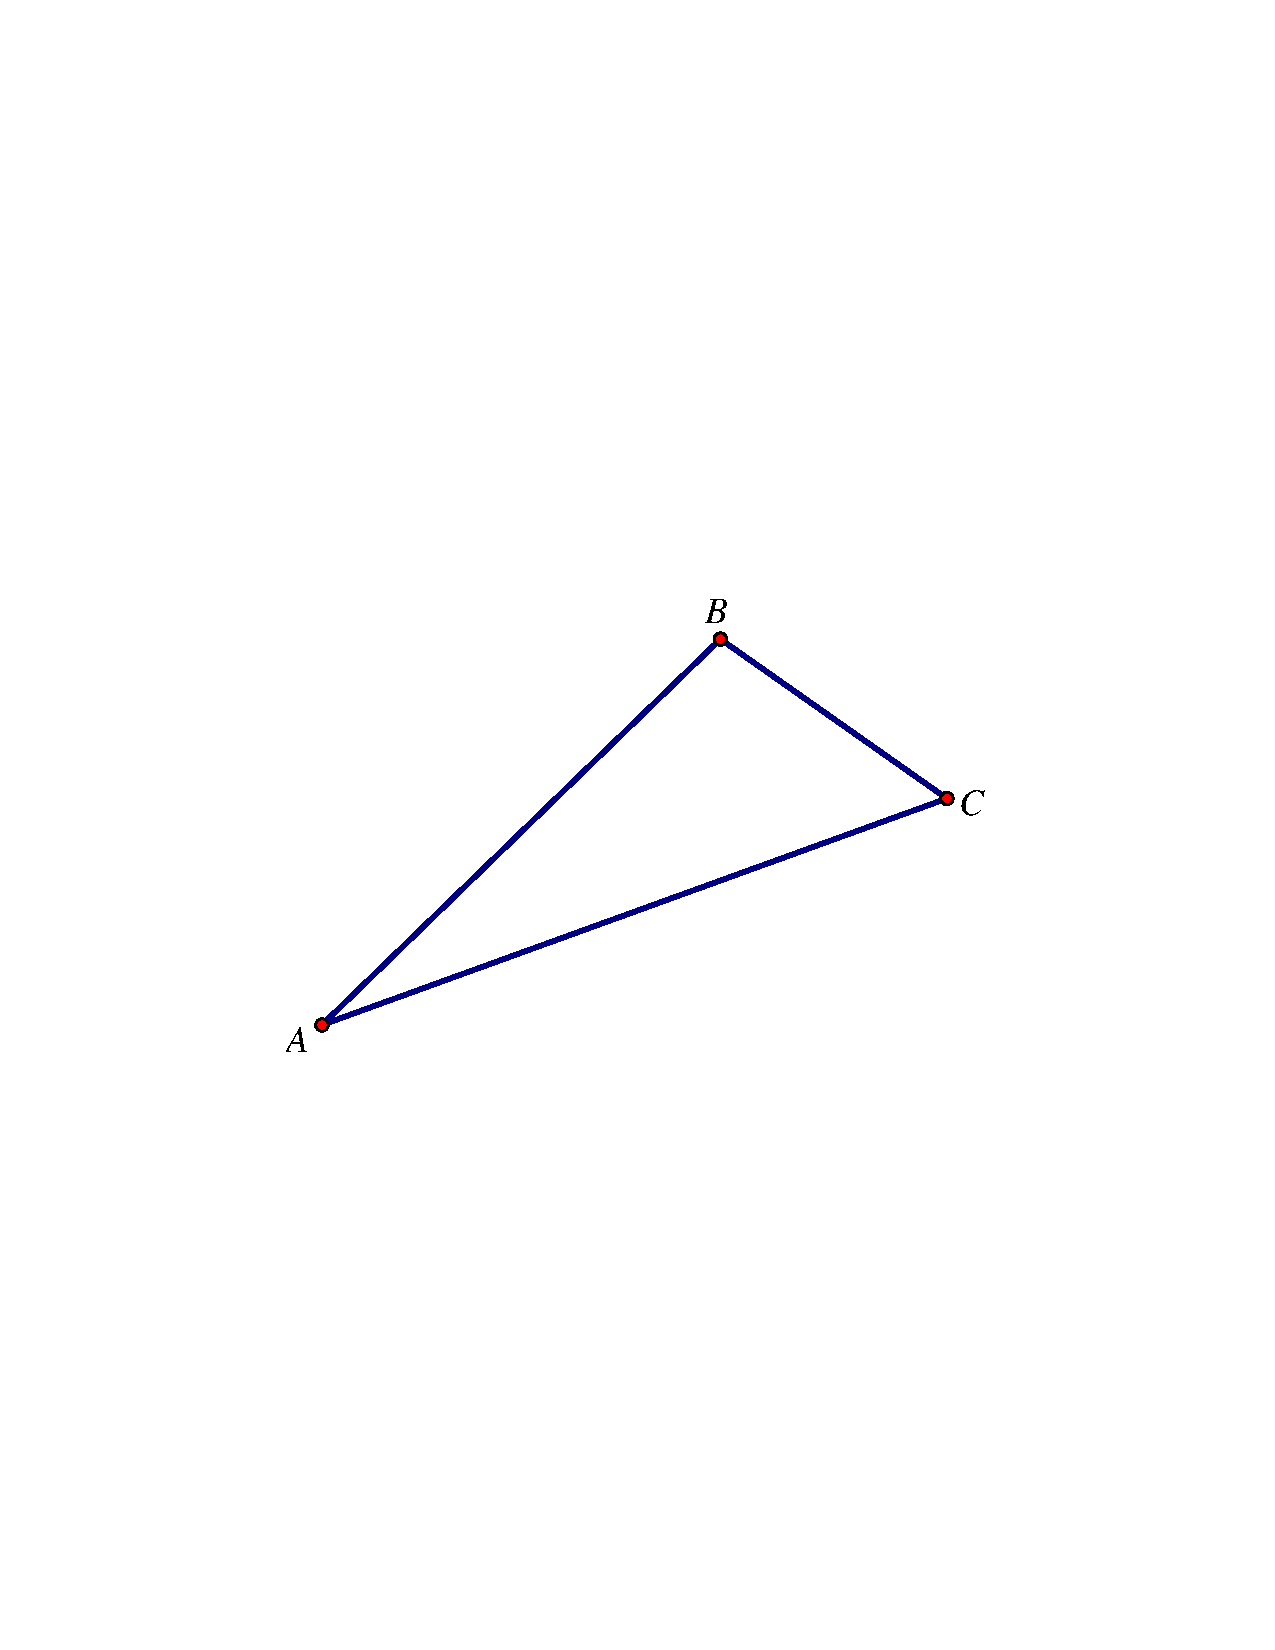
\includegraphics[scale=0.9]{obtuseTriangle.pdf}
\vfill
\end{problem}

\newpage
\begin{problem}
In the triangle below, draw the median from $C$ to $\overline{AB}$, the altitude from $C$ to $\overline{AB}$, the angle bisector of $\angle C$, and the perpendicular bisector of $\overline{AB}$. 

%\begin{enumerate}
%\item Median from $C$ to $\overline{AB}$
%\item Altitude from $C$ to $\overline{AB}$
%\item Angle bisector of $\angle C$
%\item Perpendicular bisector of $\overline{AB}$
%\end{enumerate}
%
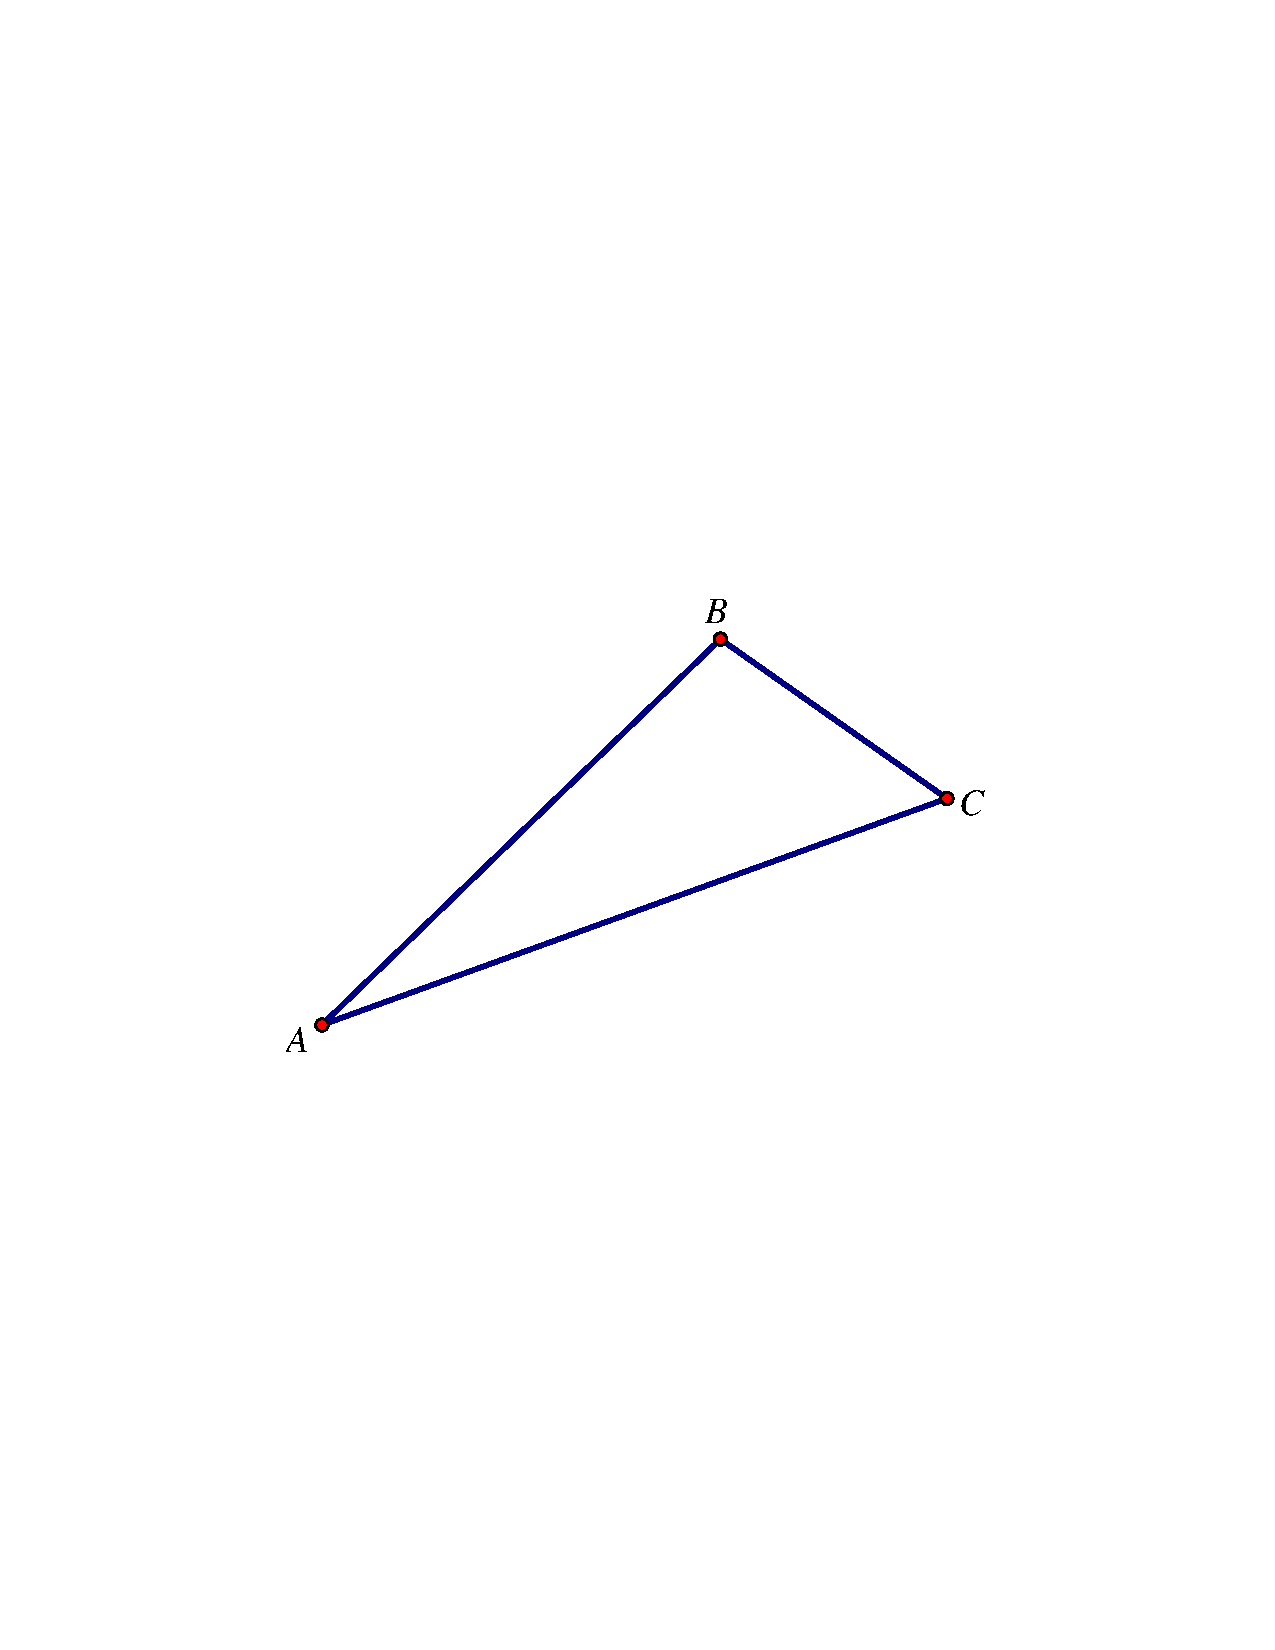
\includegraphics[scale=0.9]{obtuseTriangle.pdf}
\end{problem}


\begin{problem}
In each triangle, you should have drawn four different lines.  What might you say about a triangle for which two or more of these lines turn out to be the same?  
\vfill
\end{problem}

\end{document}

\newpage

\section{Isosceles Bisectors}

\begin{teachingnote}
Students typically draw a new line. They must choose which line they are drawing and then they must assume no additional properties.  Then they look for triangle congruence.  Median: SSS.  Altitude: HL.  Angle bisector: SAS. Perpendicular bisector: doesn't work because it might not contain the opposite vertex.  

Work through analogous ideas for the converse. 
\end{teachingnote}

\begin{theorem}[Isosceles Triangle Theorem]
If two sides of a triangle are congruent, then the angles opposite those sides are congruent. 
\end{theorem}

\begin{prob}
Prove the Isosceles Triangle Theorem.  (Hint: In a previous activity, you noticed that in most triangles the median, perpendicular bisector, angle bisector, and altitude to a side lie on four different lines.  So if you draw a new line in your diagram, be sure to decide which of these lines you are drawing.)
\end{prob}
\vfill

\begin{prob}
Use your proof to show that a median, perpendicular bisector, angle bisector, and altitude turn out to be the same line.
\end{prob}
\vfill
\newpage

\begin{prob}
Prove the Isosceles Triangle Theorem without drawing another line.  Hint:  Is there a way in which the triangle is congruent to itself? 
\end{prob}
\vfill

\begin{prob}
State the converse of the Isosceles Triangle Theorem and prove it.  
\end{prob}
\vfill
\newpage
\begin{prob}
Prove that the points on the perpendicular bisector of a segment are \emph{exactly those} that are equidistant from the endpoints of the segment.  Note that the phrase \emph{exactly those} requires that we prove a simpler statement as well as its converse:   
\begin{enumerate}
\item Prove that a point on the perpendicular bisector of a segment is equidistant from the endpoints of that segment.
\item Prove that a point that is equidistant from the endpoints of a segment lies on the perpendicular bisector of that segment.
\end{enumerate}
\end{prob}

\begin{prob}
Prove that the perpendicular bisectors of a triangle are concurrent.  Hint:  Name the intersection of two of the perpendicular bisectors and then show that it must also lie on the third one.  (This is a standard approach for showing the concurrency of three lines.)  
\end{prob}

\begin{prob}
Draw a line (neither horizontal nor vertical) and a point not on the line.  Describe how to find the \emph{exact} distance from the point to the line. 
\end{prob}

\begin{prob}
Prove that the points on an angle bisector are \emph{exactly those} that are equidistant from the sides of the angle. 
\end{prob}

\begin{prob}
Prove that the angle bisectors of a triangle are concurrent. 
\end{prob}


\newpage

\section{About Medians}
\begin{teachingnote}
Supplies:  Cardstock, thread, 12-inch rulers.
\end{teachingnote}
Here we explore several ways of thinking about the medians of triangles.  

\begin{prob}  
On cardstock, use a ruler to draw a medium-sized, non-right, non-isosceles triangle, and then cut it out as accurately as you can.  Draw two of the medians on the cutout triangle.  Draw the third median to make sure they are concurrent.  
\begin{enumerate}
\item Using a ruler, try balancing the triangle along each median.  (Ask a partner to hold the ruler steady.)  
\item Now try balancing the triangle along a line that is \emph{not} a median.  How does your line relate to the intersection of the medians?  Explain why this makes sense.  
\item Try balancing the triangle from a string at the intersection of the medians.  (Use the point of your compass to make a hole in the cardstock.)
\end{enumerate}

\end{prob}

\begin{prob}
Imagine stacking toothpicks in a triangle, as shown below.  

$$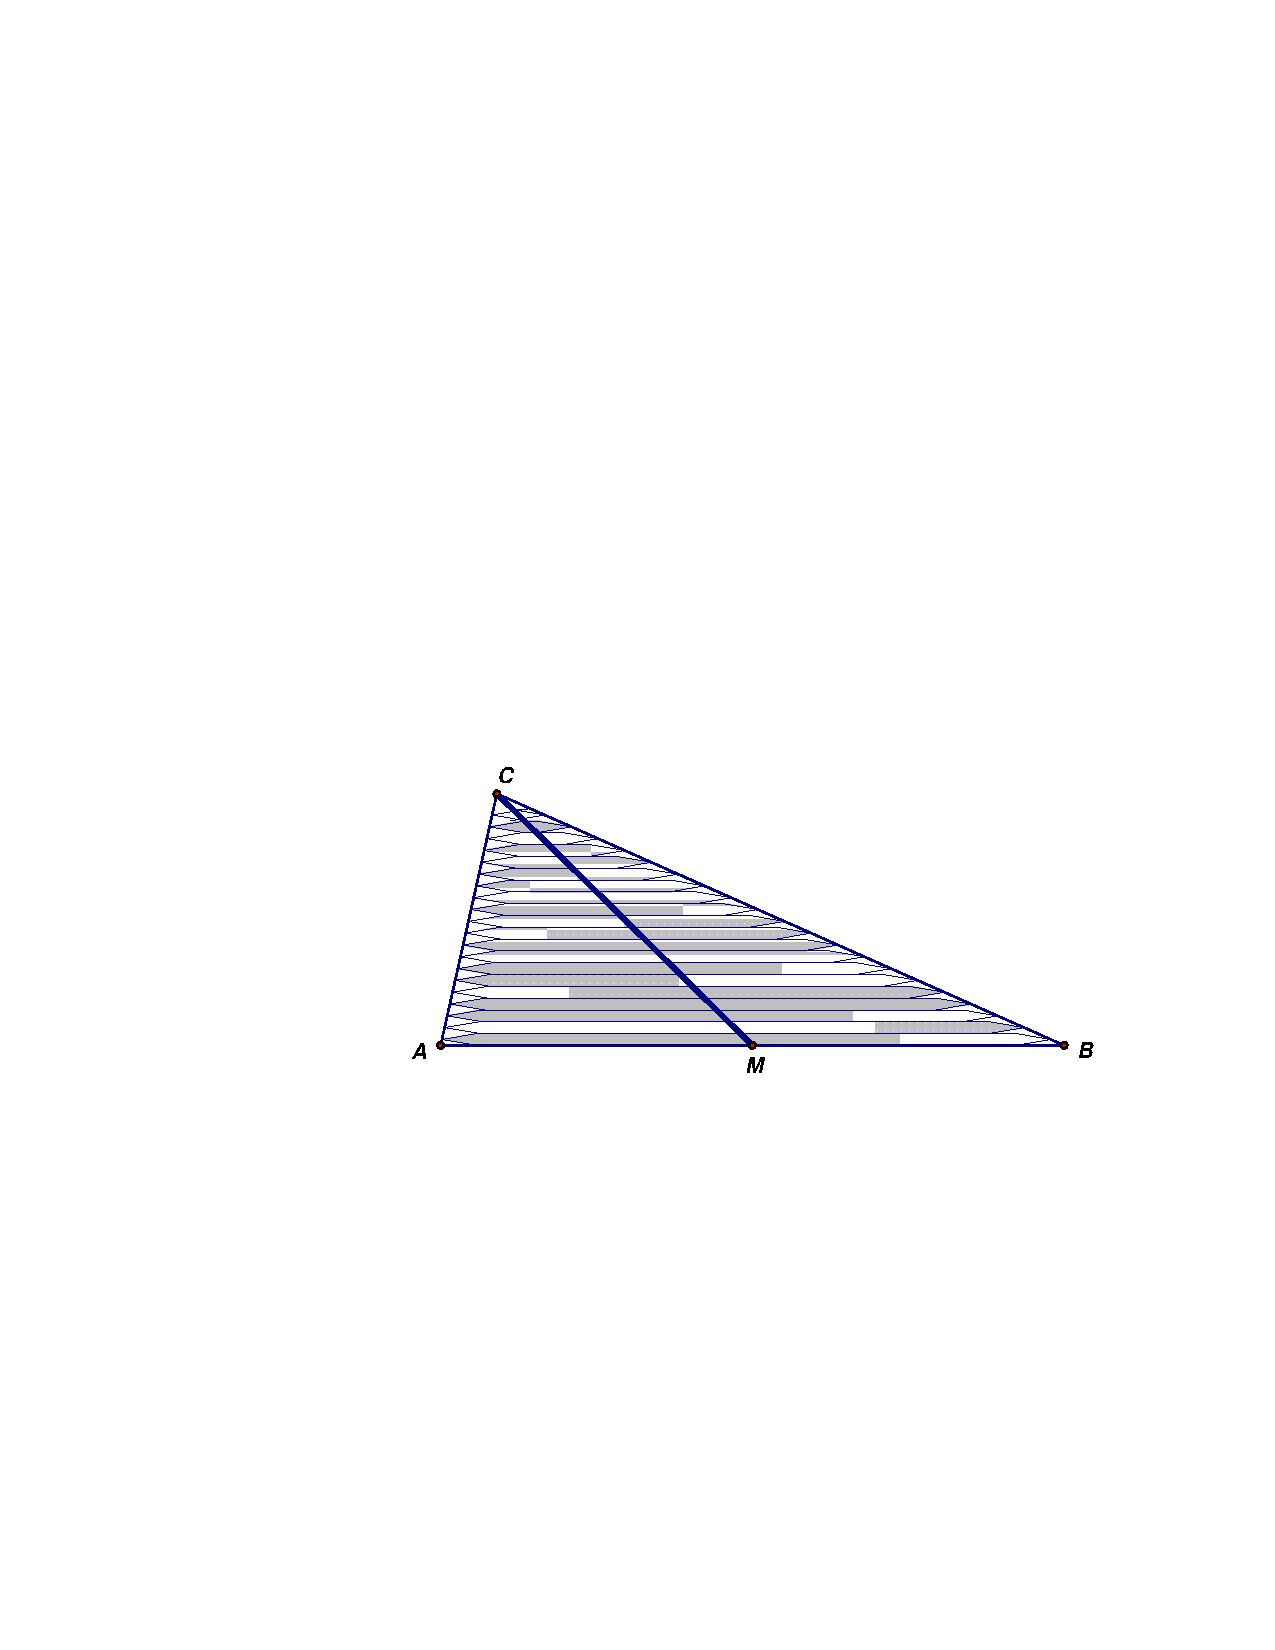
\includegraphics[width=2.5in]{../graphics/toothpicks.pdf}$$

\begin{enumerate}
\item Explain, using toothpicks, why the triangle would balance on a ruler placed along the median $\overline{CM}$.  
\item Explain, using a different collection of toothpicks, why the triangle would balance along the median to side $\overline{AC}$.  Describe how the toothpicks would need be placed, relative to side $\overline{AC}$.
\item The two medians will intersect at a point.  Explain why the triangle (without toothpicks) should balance from a string or on a pencil point at the intersection of the two medians.  
\item Use a balancing argument to explain why the third median should contain the intersection of the first two.  
\end{enumerate}
\end{prob}

\begin{prob}
The next problem uses the midsegment theorem.  A \emph{midsegment} is a line joining the midpoints of two sides.  Draw carefully a triangle and a midsegment, and use it to make a conjecture about what the midsegment theorem says.  (We will prove the theorem later.)
\end{prob}

\begin{teachingnote}
\textbf{Midsegment Theorem:}  A midsegment in a triangle is parallel to and half the length of the corresponding side.
\end{teachingnote}

\begin{prob}
Use the picture below to show that a pair of medians intersects at a point 2/3 of the way from the vertex to the opposite side.  Then use that fact to argue that the three medians must be concurrent.  
$$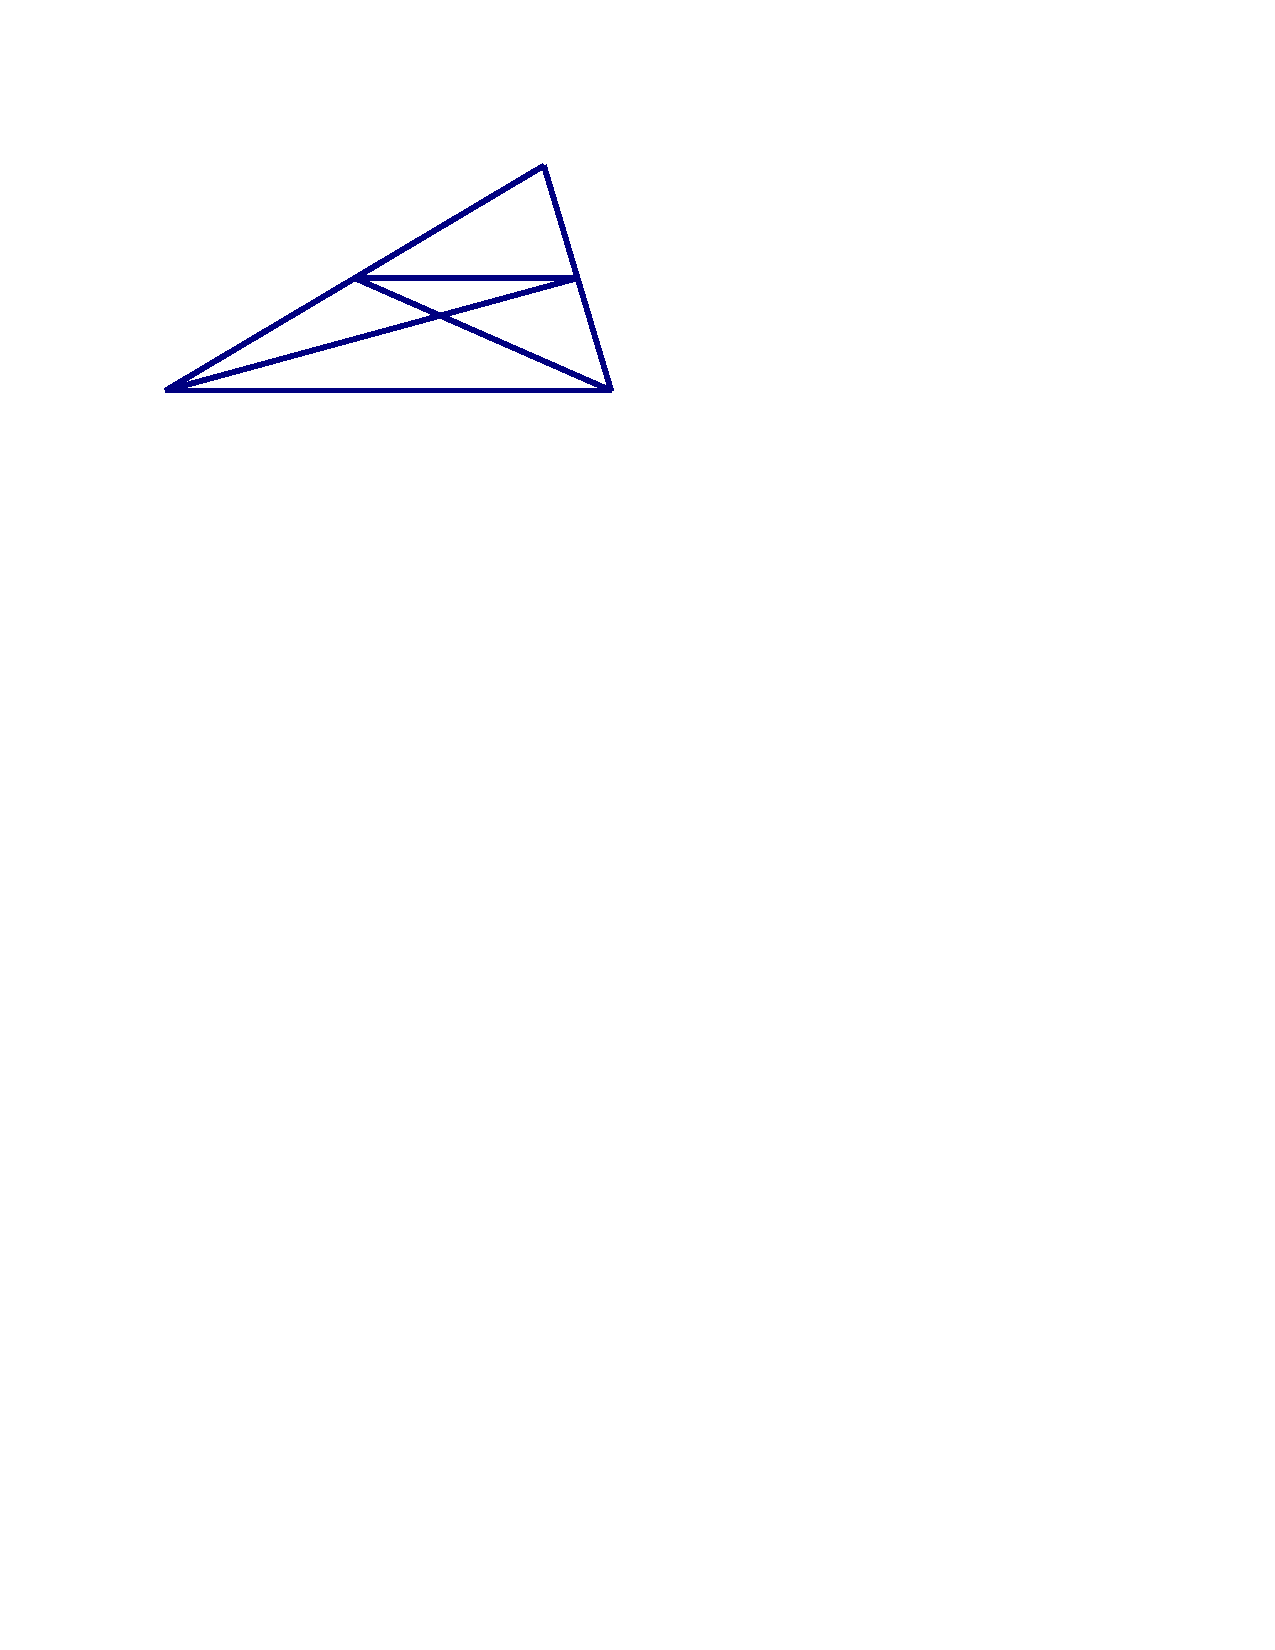
\includegraphics[width=2.5in]{../graphics/median1.pdf}$$
\end{prob}

\begin{prob}
Imagine a triangle made of nearly weightless material with one-pound weights placed at each of the vertices, $A$, $B$, and $C$.  
\begin{enumerate}
\item Explain why the triangle will balance on a ruler along the median to side $\overline{AB}$.  
\item Explain why the triangle will continue to balance along the median when the masses at $A$ and $B$ are both moved to the midpoint of $\overline{AB}$.  
\item Now imagine trying to balance the triangle at a single point along the median.  Where will it balance?  Use the phrase ``weighted average'' to explain your reasoning.   
\end{enumerate}
\end{prob}

\begin{prob}
Using the picture below, explain why the medians of the large triangle are also medians of the medial triangle.  Then explain how repeating this process indefinitely proves that the medians are concurrent.
$$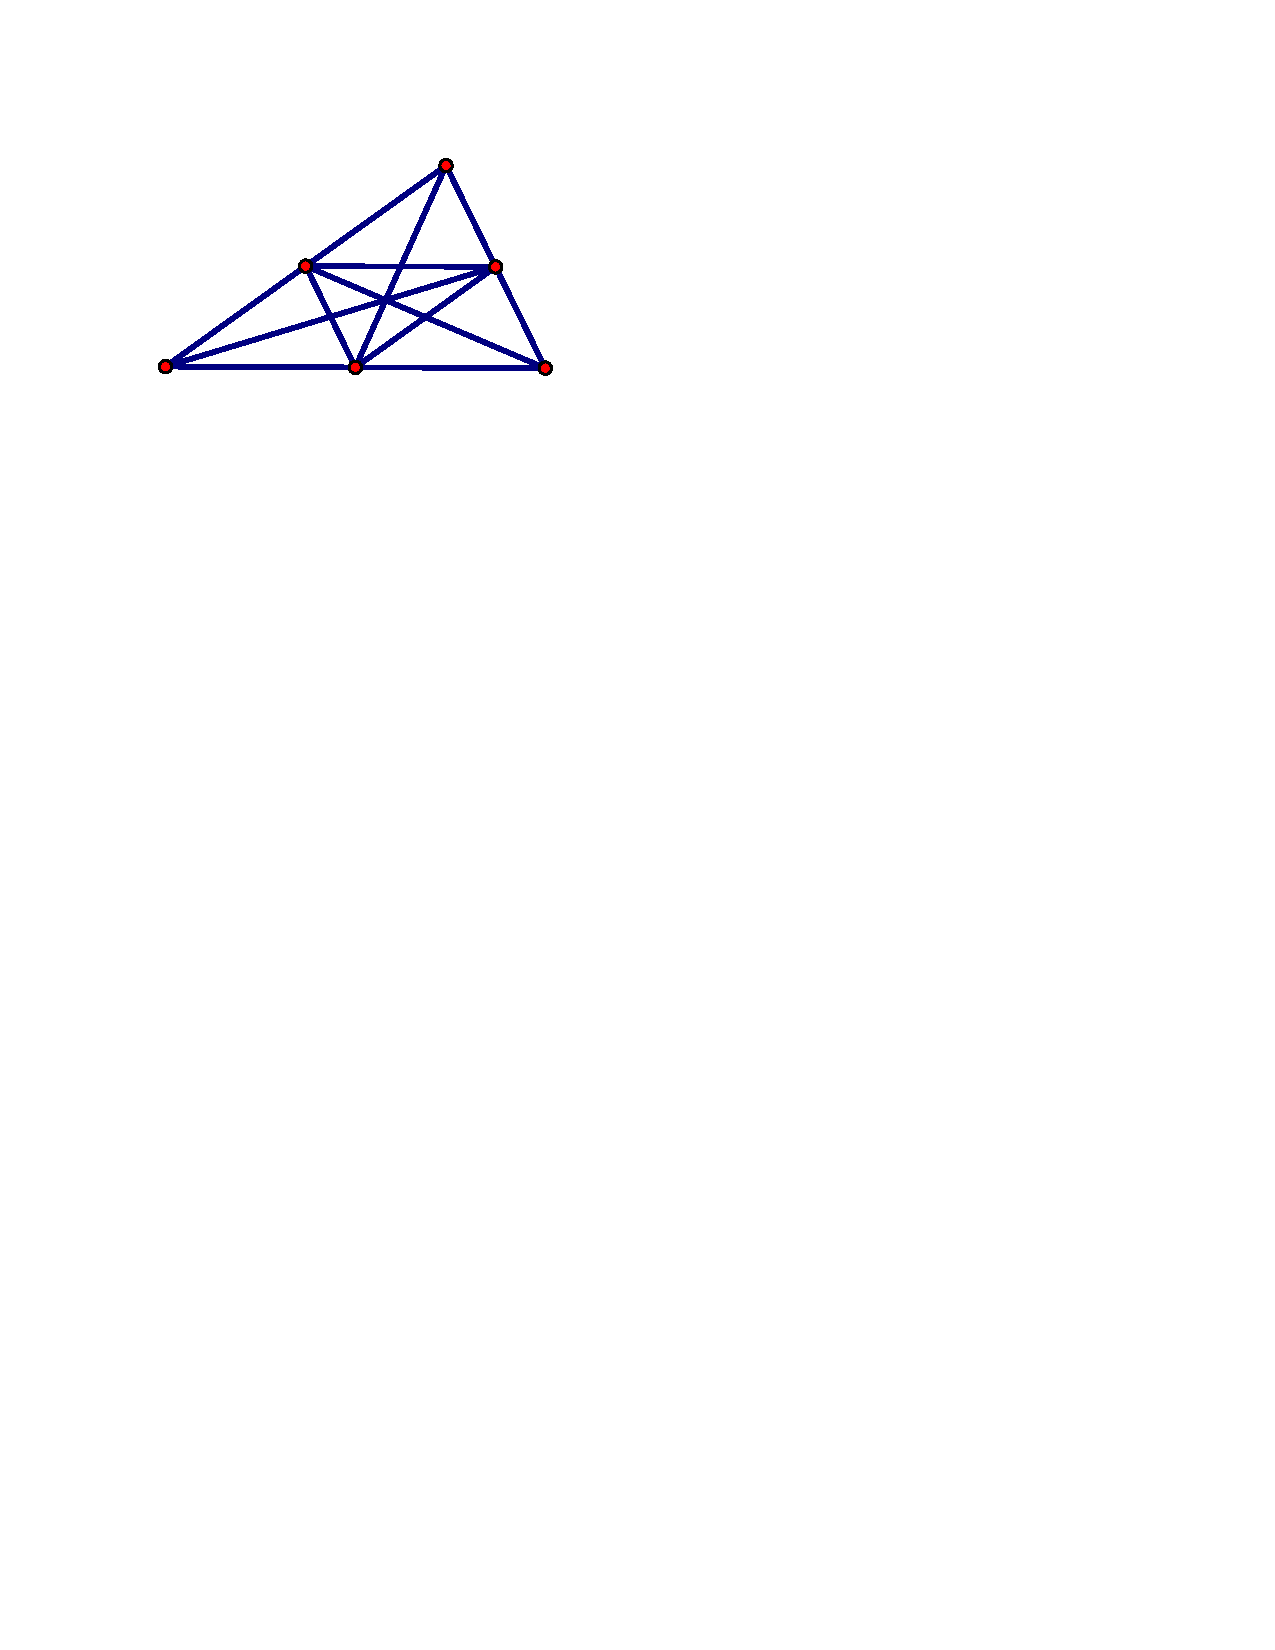
\includegraphics[width=2.5in]{../graphics/median2.pdf}$$
\end{prob}
 




%\newpage
\section{The Euler Line and the Nine-Point Circle} 

\begin{prob} 
Use \textsl{GeoGebra} to make the following constructions on an arbitrary triangle.  
\begin{itemize}
\itemsep -3pt
\item Construct the circumcenter of the 
triangle. Hide all extraneous lines and points. Label this point $C$.
\item Construct the centroid of the same triangle. Hide
all extraneous lines and points. Label this point $N$.
\item Construct the orthocenter of the same triangle. Hide
all extraneous lines and points. Label this point $O$.
\item Connect $C$ and $O$ with a segment. 
\end{itemize}
Did a miracle happen?  Describe what you notice about the 
segments $\overline{CN}$ and $\overline{ON}$.    
\end{prob}
\vfill
\begin{prob}
Keeping the same triangle as used in the previous problem, use \textsl{GeoGebra} to make the following construction:  
\begin{itemize}
\itemsep -3pt
\item Mark the midpoint of the segment that connects $C$ and $O$. Label this point $M$.
\item Mark the midpoints of each side. (Hint: Try to ``unhide'' those you have used already.)
\item Mark where the altitudes
meet the lines containing the sides of the triangle. Hide all
extraneous lines and points.
\item Mark the midpoints of
the segments joining the orthocenter and the vertices. Hide all
extraneous lines and points.
\item Draw a circle centered at $M$ that goes through one of the midpoints of the triangle.
\end{itemize}
 Did a miracle happen?  Describe what you notice.  
\end{prob}
\vfill
\begin{prob}
Complete the following sentences:  
\begin{enumerate}
\item The \emph{Euler line} contains the following points:  
%\vspace{.5in}
\vfill
\item The \emph{nine-point circle} contains the following points:  
\end{enumerate}
\end{prob}
\vfill

%\newpage
\section{Apothem} %% remove * if added to main notes

Draw yourself a picture of a happy little equilateral triangle. Do
it---seriously.  Some people might call an equilateral triangle a
\textit{regular 3-gon}.

\begin{prob} 
What is an \textit{$n$-gon}? Give some relevant and revealing examples
and nonexamples.
\end{prob}

\begin{prob} 
When discussing $n$-gons, what are the allowable values for $n$?
\end{prob}

\begin{prob} 
What is a \textit{regular $n$-gon}? Give some relevant and revealing
examples and nonexamples.
\end{prob}


\begin{definition} 
A segment connecting the intersection of any two perpendicular
bisectors of sides of a polygon to either of those sides is called an
\textbf{apothem}\index{apothem}.
\end{definition}

\begin{prob}
Can you tell me in English what this defintion says? Provide some
examples of this definition in action.
\end{prob}



\begin{prob} 
Now consider some regular $n$-gon. Use \textsl{GeoGebra} to construct
apothems.
\end{prob}



\begin{prob}
Given a polygon, if you know the side length and the length of the
apothems, how do you find the area of your polygon? 
\end{prob}


\begin{prob}
Fix a value for $n$. Then use \textsl{GeoGebra} to help you fill in
the following table for various lengths of apothems.
\begin{center}
\begin{tabular}{|c||c|c|c|c|}\hline
$n$-gon & Apothem & Side & Perimeter & Area  \\\hline\hline
 \rule[0mm]{0mm}{7mm}\hspace{15mm}  &  & &  &  \\ \hline
 \rule[0mm]{0mm}{7mm}\hspace{15mm} &  & &  &  \\ \hline
 \rule[0mm]{0mm}{7mm}\hspace{15mm} &  & &  &  \\ \hline
 \rule[0mm]{0mm}{7mm}\hspace{15mm} &  & &  &  \\ \hline
 \rule[0mm]{0mm}{7mm}\hspace{15mm} &  & &  &  \\ \hline
 \rule[0mm]{0mm}{7mm}\hspace{15mm} &  & &  &  \\ \hline
 \rule[0mm]{0mm}{7mm}\hspace{15mm} &  & &  &  \\ \hline
\end{tabular}
\end{center}
\end{prob}

\begin{prob}
If $a$ is the length of the apothem, $P$ is the perimeter, and $A$ is
the area of the regular polygon, can you give a formula relating all
three of these quantities?
%\[
%A = \frac{pa}{2}
%\]
\end{prob}


%\documentclass[handout]{ximera}
\documentclass[nooutcomes]{ximera}

\usepackage{gensymb}
\usepackage{tabularx}
\usepackage{mdframed}
\usepackage{pdfpages}
%\usepackage{chngcntr}

\let\problem\relax
\let\endproblem\relax

\newcommand{\property}[2]{#1#2}




\newtheoremstyle{SlantTheorem}{\topsep}{\fill}%%% space between body and thm
 {\slshape}                      %%% Thm body font
 {}                              %%% Indent amount (empty = no indent)
 {\bfseries\sffamily}            %%% Thm head font
 {}                              %%% Punctuation after thm head
 {3ex}                           %%% Space after thm head
 {\thmname{#1}\thmnumber{ #2}\thmnote{ \bfseries(#3)}} %%% Thm head spec
\theoremstyle{SlantTheorem}
\newtheorem{problem}{Problem}[]

%\counterwithin*{problem}{section}



%%%%%%%%%%%%%%%%%%%%%%%%%%%%Jenny's code%%%%%%%%%%%%%%%%%%%%

%%% Solution environment
%\newenvironment{solution}{
%\ifhandout\setbox0\vbox\bgroup\else
%\begin{trivlist}\item[\hskip \labelsep\small\itshape\bfseries Solution\hspace{2ex}]
%\par\noindent\upshape\small
%\fi}
%{\ifhandout\egroup\else
%\end{trivlist}
%\fi}
%
%
%%% instructorIntro environment
%\ifhandout
%\newenvironment{instructorIntro}[1][false]%
%{%
%\def\givenatend{\boolean{#1}}\ifthenelse{\boolean{#1}}{\begin{trivlist}\item}{\setbox0\vbox\bgroup}{}
%}
%{%
%\ifthenelse{\givenatend}{\end{trivlist}}{\egroup}{}
%}
%\else
%\newenvironment{instructorIntro}[1][false]%
%{%
%  \ifthenelse{\boolean{#1}}{\begin{trivlist}\item[\hskip \labelsep\bfseries Instructor Notes:\hspace{2ex}]}
%{\begin{trivlist}\item[\hskip \labelsep\bfseries Instructor Notes:\hspace{2ex}]}
%{}
%}
%% %% line at the bottom} 
%{\end{trivlist}\par\addvspace{.5ex}\nobreak\noindent\hung} 
%\fi
%
%


\let\instructorNotes\relax
\let\endinstructorNotes\relax
%%% instructorNotes environment
\ifhandout
\newenvironment{instructorNotes}[1][false]%
{%
\def\givenatend{\boolean{#1}}\ifthenelse{\boolean{#1}}{\begin{trivlist}\item}{\setbox0\vbox\bgroup}{}
}
{%
\ifthenelse{\givenatend}{\end{trivlist}}{\egroup}{}
}
\else
\newenvironment{instructorNotes}[1][false]%
{%
  \ifthenelse{\boolean{#1}}{\begin{trivlist}\item[\hskip \labelsep\bfseries {\Large Instructor Notes: \\} \hspace{\textwidth} ]}
{\begin{trivlist}\item[\hskip \labelsep\bfseries {\Large Instructor Notes: \\} \hspace{\textwidth} ]}
{}
}
{\end{trivlist}}
\fi


%% Suggested Timing
\newcommand{\timing}[1]{{\bf Suggested Timing: \hspace{2ex}} #1}




\hypersetup{
    colorlinks=true,       % false: boxed links; true: colored links
    linkcolor=blue,          % color of internal links (change box color with linkbordercolor)
    citecolor=green,        % color of links to bibliography
    filecolor=magenta,      % color of file links
    urlcolor=cyan           % color of external links
}

\title{Verifying Our Constructions}
\author{Bart Snapp and Brad Findell}

\outcome{Learning outcome goes here.}

\begin{document}
\begin{abstract}
  We use basic theorems to verify our Euclidean compass-and-straightedge constructions.
\end{abstract}
\maketitle

\begin{teachingnote}
This activity ties together ideas that have been used informally so far.  
\end{teachingnote}

When we do our compass-and-straightedge constructions, we should take
care to verify that they actually work as advertised. We'll walk you
through this process. To start, remember what a circle is:

\begin{definition} 
A \textbf{circle} is the set of points that are a fixed distance from
a given point.
\end{definition}

\begin{problem} Is the center of a circle part of the circle?
\end{problem}

\begin{problem} 
Construct an equilateral triangle.  Why does this construction work?
\end{problem}




Now recall the SSS Theorem:

\begin{theorem}[SSS] 
Specifying three sides uniquely determines a triangle.
\end{theorem}



\begin{problem} Now we'll analyze the construction for copying angles. 
\begin{enumerate}
\item Use a compass and straightedge construction to duplicate an
  angle. Explain how you are really just ``measuring'' the sides of
  some triangle.
\item In light of the SSS Theorem, can you explain why the
  construction used to duplicate an angle works?
\end{enumerate}
\end{problem}


\begin{problem} Now we'll analyze the construction for bisecting angles.
\begin{enumerate}
\item Use compass and straightedge construction to bisect an
  angle. Explain how you are really just constructing (two)
  isosceles triangles. Draw these isosceles triangles in your figure.
\item Find two more triangles on either side of your angle bisector where
  you may use the SSS Theorem to argue that they have equal side
  lengths and therefore equal angle measures.
\item Can you explain why the construction used to bisect angles
  works?
\end{enumerate}
\end{problem}


Recall the SAS Theorem:

\begin{theorem}[SAS] 
Specifying two sides and the angle between them uniquely determines a
triangle.
\end{theorem}


\begin{problem} Now we'll analyze the construction for bisecting segments.
\begin{enumerate} 
\item Use a compass and straightedge construction to bisect a
  segment. Explain how you are really just constructing two
  isosceles triangles.
\item Note that the bisector divides each of the above isosceles
  triangles in half. Find two triangles on either side of your
  bisector where you may use the SAS Theorem to argue that they have
  equal side lengths and angle measures.
\item Can you explain why the construction used to bisect segments
  works?
\end{enumerate}
\end{problem}




\begin{problem} 
Now we'll analyze the construction of a perpendicular line through a
point not on the line.
\begin{enumerate}
\item Use a compass and straightedge construction to construct a
  perpendicular through a point. Explain how you are really just
  constructing an isosceles triangle.
\item Find two triangles in your construction where you may use the
  SAS Theorem to argue that they have equal side lengths and angle
  measures.
\item Can you explain why the construction used to construct a
  perpendicular through a point works?
\end{enumerate}
\end{problem}
\end{document}


\newpage
\section{Of Angles and Circles} %%remove * if added to notes!

\begin{teachingnote}
A chord defines two central angles and two arcs: a ``standard'' and reflex angle pair, corresponding to a minor and a major arc.  So in this activity, central and inscribed angles intercept arcs rather than chords.
\end{teachingnote}

In this activity we are going to look at pictures and see if we can
explain how they ``prove'' theorems.

\begin{theorem} 
Any triangle inscribed in a circle and having the diameter as a side is a
right triangle.
\end{theorem}

\begin{prob}
Can you tell me in English what this theorem says? Provide some
examples of this theorem in action.
\end{prob}

\begin{prob} 
Here is a series of pictures, designed to be read from left to right.
\[
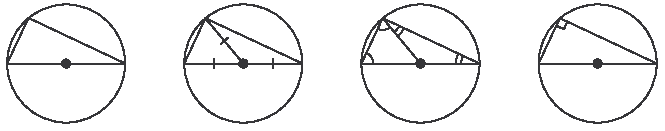
\includegraphics{../graphics/pbpcircthm1.pdf}
\]
Explain how these pictures ``prove'' the above theorem. In the process
of your explanation, you may need to label parts of the pictures and
do some algebra.
\end{prob}

\begin{definition}
A \emph{chord} in a circle defines two {arcs}, each of which corresponds to a {central angle}.  The \emph{measure} of the arc is defined to be the measure of the corresponding central angle.  
\end{definition}

\begin{prob}
Can you tell me in English what this definition says? Use pictures to demonstrate what the fancy words mean.  
\end{prob}

\begin{theorem} 
Given an arc of a circle, the central angle corresponding to this arc is
twice any inscribed angle intercepting this arc.
\end{theorem}

I'll play nice here and give you a picture of this theorem in action:
\[
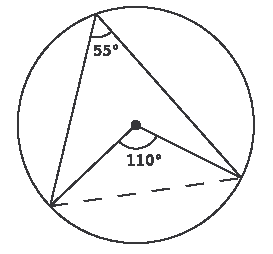
\includegraphics[scale=0.8]{../graphics/pbpcircthm2eg.pdf}
\]

\begin{prob}
Can you tell me in English what this theorem says?  Specifically, what is meant by
\textit{inscribed angle}?  And why does it say ``any inscribed angle''?
\end{prob}

\begin{prob} 
For one possible line of reasoning, consider this series of pictures, designed to be read from left to right.
\[
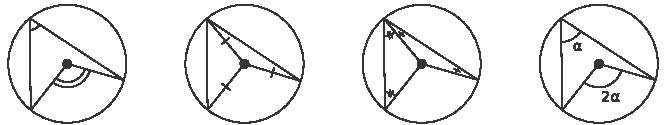
\includegraphics{../graphics/pbpcircthm2.pdf}
\]

Explain how these pictures ``prove'' the above theorem. In the process
of your explanation, you may need to label parts of the pictures and
do some algebra.
\end{prob}


\begin{prob}
Not all inscribed angles look like those in the previous picture.  Consider the following pictures:  
\[
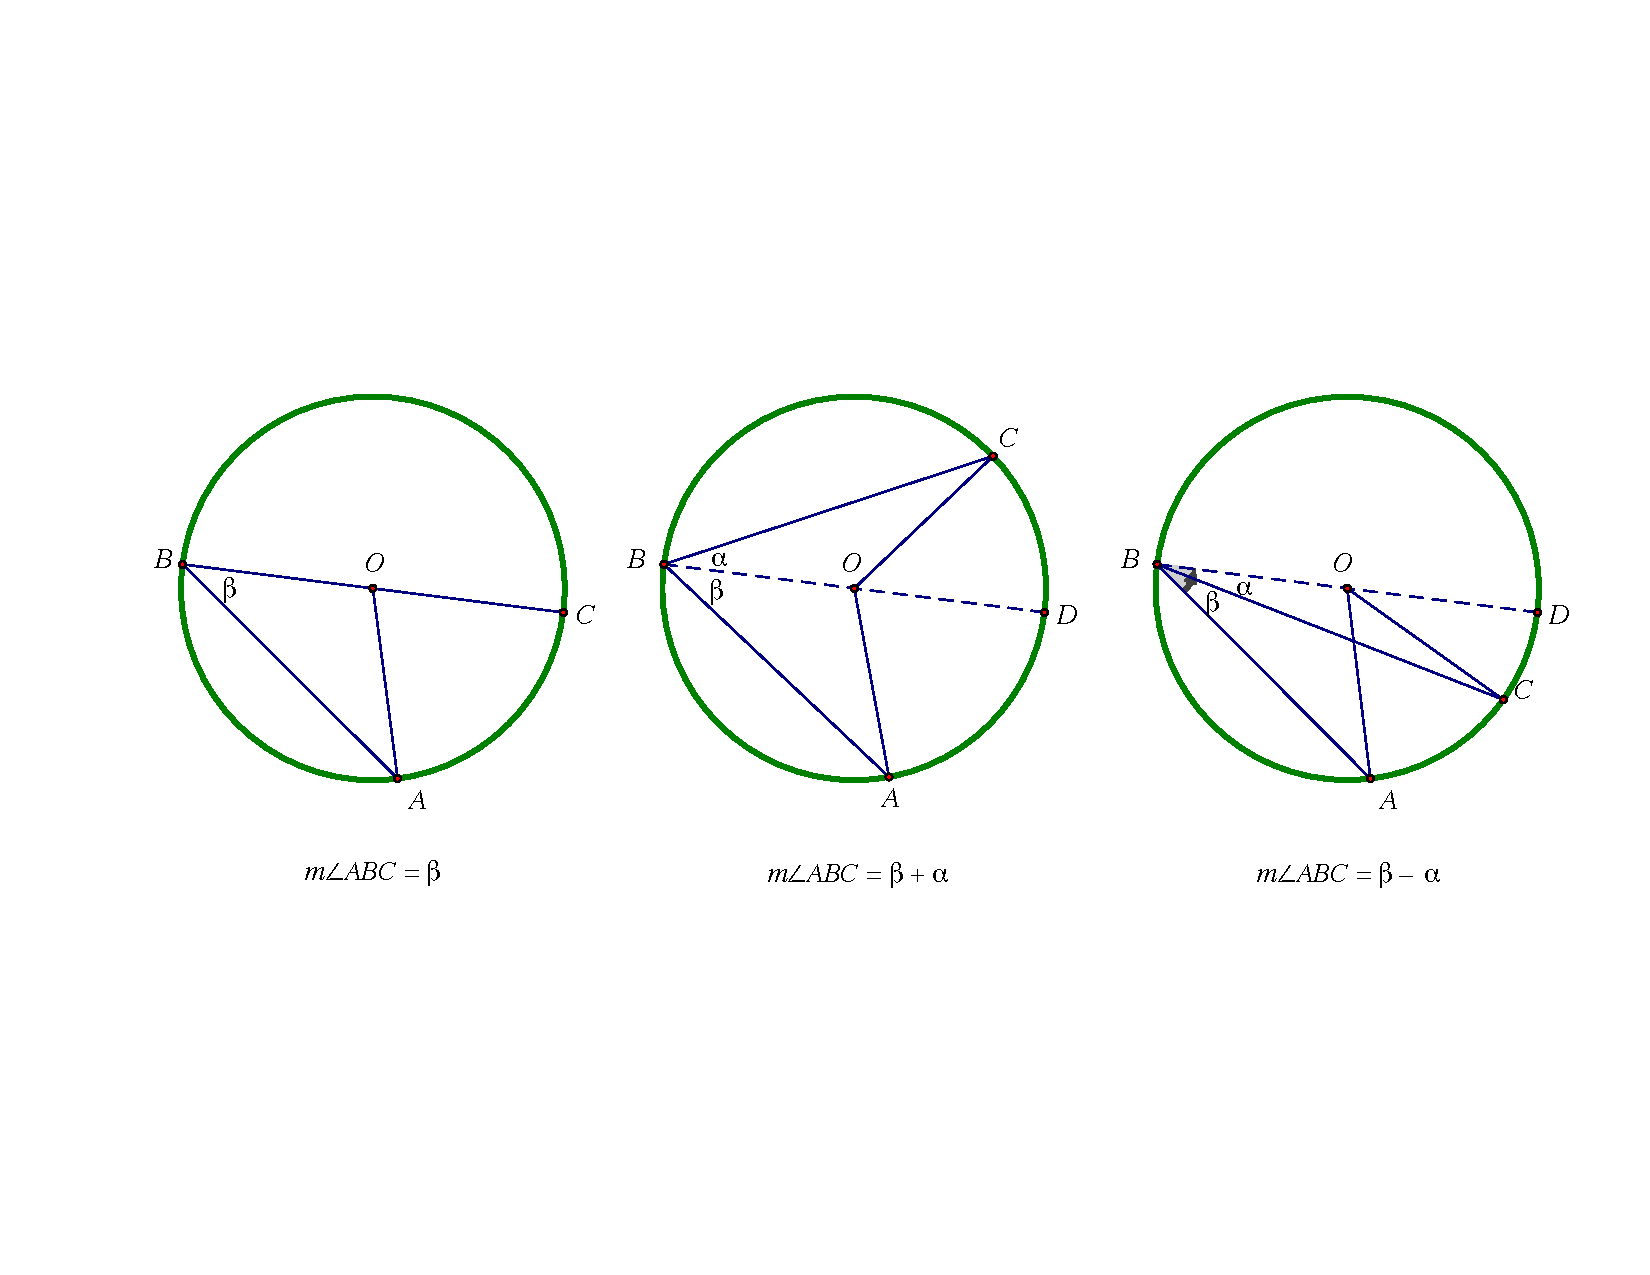
\includegraphics[width=5in]{../graphics/inscribedAngle.pdf}
\]
\
\begin{enumerate}
\item In each of the pictures, find and explain the relationship between $m\angle ABC$ and $m\angle AOC$.
\item Explain why any inscribed angle must fit one of these three cases.  
\end{enumerate}
% Can you show $m\angle AXB = \frac{1}{2}m\angle AOB$ for the sequence of cases below.  
\end{prob}

\begin{teachingnote}
The idea is rather simple, though it is not easy to see, especially in the third figure.  When the center is inside the inscribed angle, you can consider it to be the *sum* of two angles, each of which has one side through the center.  When the center is outside the inscribed angle, you can consider it to be the *difference* of two angles, each of which has one side through the center.  
\end{teachingnote}

\begin{corollary} 
Given an arc of a circle, all inscribed angles intercepting this arc are congruent.
\end{corollary}

\begin{prob} 
Firstly---what the heck is a corollary? Secondly---what is it saying?
Thirdly---why is it true?
\end{prob}


%\documentclass[handout]{ximera}
\documentclass[nooutcomes]{ximera}

\usepackage{gensymb}
\usepackage{tabularx}
\usepackage{mdframed}
\usepackage{pdfpages}
%\usepackage{chngcntr}

\let\problem\relax
\let\endproblem\relax

\newcommand{\property}[2]{#1#2}




\newtheoremstyle{SlantTheorem}{\topsep}{\fill}%%% space between body and thm
 {\slshape}                      %%% Thm body font
 {}                              %%% Indent amount (empty = no indent)
 {\bfseries\sffamily}            %%% Thm head font
 {}                              %%% Punctuation after thm head
 {3ex}                           %%% Space after thm head
 {\thmname{#1}\thmnumber{ #2}\thmnote{ \bfseries(#3)}} %%% Thm head spec
\theoremstyle{SlantTheorem}
\newtheorem{problem}{Problem}[]

%\counterwithin*{problem}{section}



%%%%%%%%%%%%%%%%%%%%%%%%%%%%Jenny's code%%%%%%%%%%%%%%%%%%%%

%%% Solution environment
%\newenvironment{solution}{
%\ifhandout\setbox0\vbox\bgroup\else
%\begin{trivlist}\item[\hskip \labelsep\small\itshape\bfseries Solution\hspace{2ex}]
%\par\noindent\upshape\small
%\fi}
%{\ifhandout\egroup\else
%\end{trivlist}
%\fi}
%
%
%%% instructorIntro environment
%\ifhandout
%\newenvironment{instructorIntro}[1][false]%
%{%
%\def\givenatend{\boolean{#1}}\ifthenelse{\boolean{#1}}{\begin{trivlist}\item}{\setbox0\vbox\bgroup}{}
%}
%{%
%\ifthenelse{\givenatend}{\end{trivlist}}{\egroup}{}
%}
%\else
%\newenvironment{instructorIntro}[1][false]%
%{%
%  \ifthenelse{\boolean{#1}}{\begin{trivlist}\item[\hskip \labelsep\bfseries Instructor Notes:\hspace{2ex}]}
%{\begin{trivlist}\item[\hskip \labelsep\bfseries Instructor Notes:\hspace{2ex}]}
%{}
%}
%% %% line at the bottom} 
%{\end{trivlist}\par\addvspace{.5ex}\nobreak\noindent\hung} 
%\fi
%
%


\let\instructorNotes\relax
\let\endinstructorNotes\relax
%%% instructorNotes environment
\ifhandout
\newenvironment{instructorNotes}[1][false]%
{%
\def\givenatend{\boolean{#1}}\ifthenelse{\boolean{#1}}{\begin{trivlist}\item}{\setbox0\vbox\bgroup}{}
}
{%
\ifthenelse{\givenatend}{\end{trivlist}}{\egroup}{}
}
\else
\newenvironment{instructorNotes}[1][false]%
{%
  \ifthenelse{\boolean{#1}}{\begin{trivlist}\item[\hskip \labelsep\bfseries {\Large Instructor Notes: \\} \hspace{\textwidth} ]}
{\begin{trivlist}\item[\hskip \labelsep\bfseries {\Large Instructor Notes: \\} \hspace{\textwidth} ]}
{}
}
{\end{trivlist}}
\fi


%% Suggested Timing
\newcommand{\timing}[1]{{\bf Suggested Timing: \hspace{2ex}} #1}




\hypersetup{
    colorlinks=true,       % false: boxed links; true: colored links
    linkcolor=blue,          % color of internal links (change box color with linkbordercolor)
    citecolor=green,        % color of links to bibliography
    filecolor=magenta,      % color of file links
    urlcolor=cyan           % color of external links
}

\title{More Circles}
\author{Bart Snapp and Brad Findell}

\outcome{Learning outcome goes here.}

\begin{document}
\begin{abstract}
  We think about circles that have certain relations to other shapes.
\end{abstract}
\maketitle

\begin{teachingnote}
This first problem is very difficult because students have to draw pictures that are clearly wrong.  Pick and choose from among the remaining problems, which might benefit from scaffolding to make them more ``activity like.''

The first problem is made considerably easier by first proving that the shortest distance from a point to a line is along a perpendicular.  That is proven indirectly.  Then Problem 1 is pretty straightforward from the definition of a circle as the set of points that are equidistant from a center.  All other points on the line must be a greater distance from the center.
\end{teachingnote}

\begin{problem}
Given a line and a point not on the line, prove that the perpendicular is unique. 

Prove the perpendicular is the shortest distance from the point to the line.  

\fixnote{Edit this.} 
\end{problem}

\begin{problem}
Prove: The radius of a circle is perpendicular to the tangent where the radius intersects the circle.  Hint:  Suppose not. 
\vfill
\end{problem}

\begin{problem}
Suppose an angle circumscribes a circle, as shown below.  Find a relationship between the measure of the angle and the measure of the central angle intercepted by the same chord.
\begin{image}
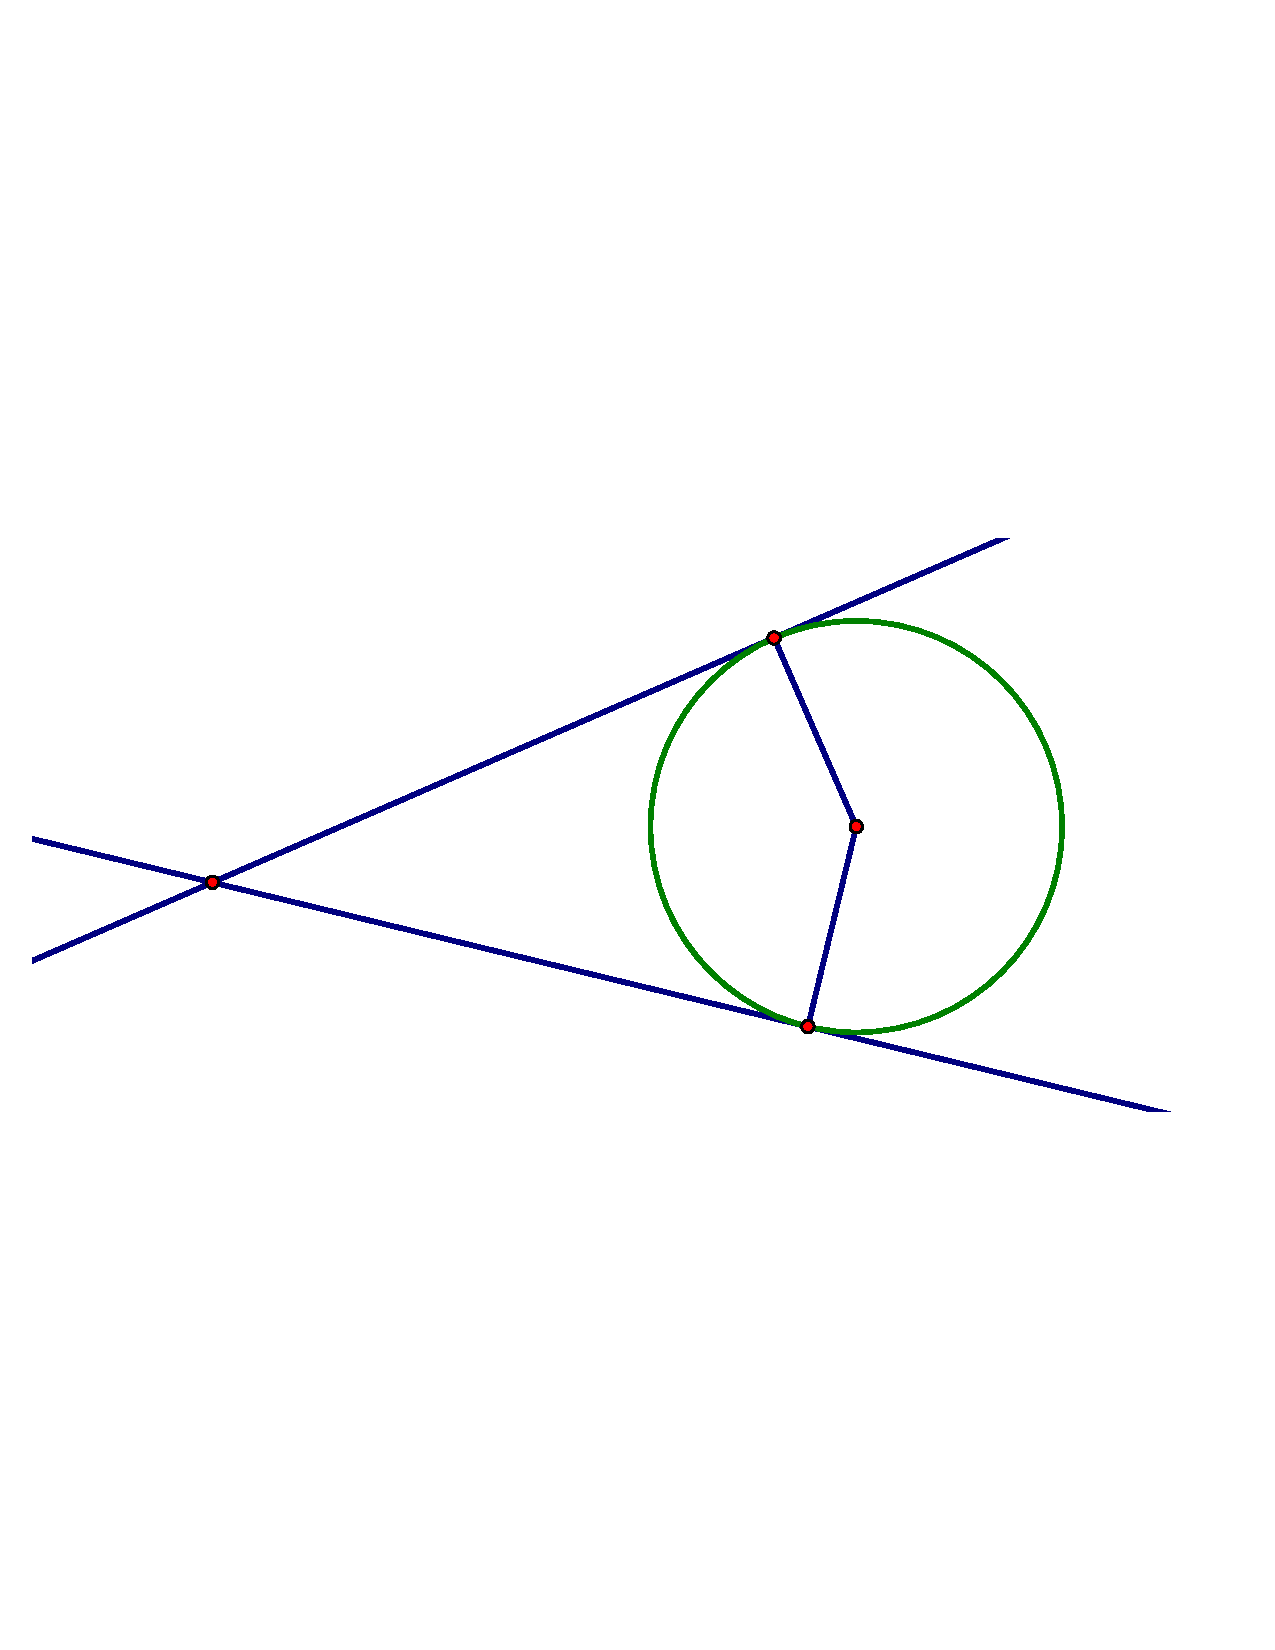
\includegraphics[width=2.5in]{circumscribedAngle.pdf}
\end{image}
\vfill
\end{problem}

\newpage

\begin{problem}
Show that, given any three non-collinear points in the Euclidean
plane, there is a unique circle passing through the three points.
\vfill
\end{problem}

\begin{problem}
Draw four points in the Euclidean plane, no three of which are collinear, that cannot lie on a single circle.  Explain your reasoning. 
\vfill
\end{problem}

\newpage
\begin{problem}
Using a compass, draw a large circle, and inscribe a quadrilateral in the circle.  Measure the four angles.  Repeat with another circle and quadrilateral.  What do you notice?  Identify a condition on any quadrilateral that is inscribed in a circle.  Now prove it.  
\vfill
\end{problem}

\begin{problem}
Construct a tangent line to a circle from a point outside the given circle.
%\begin{image}
%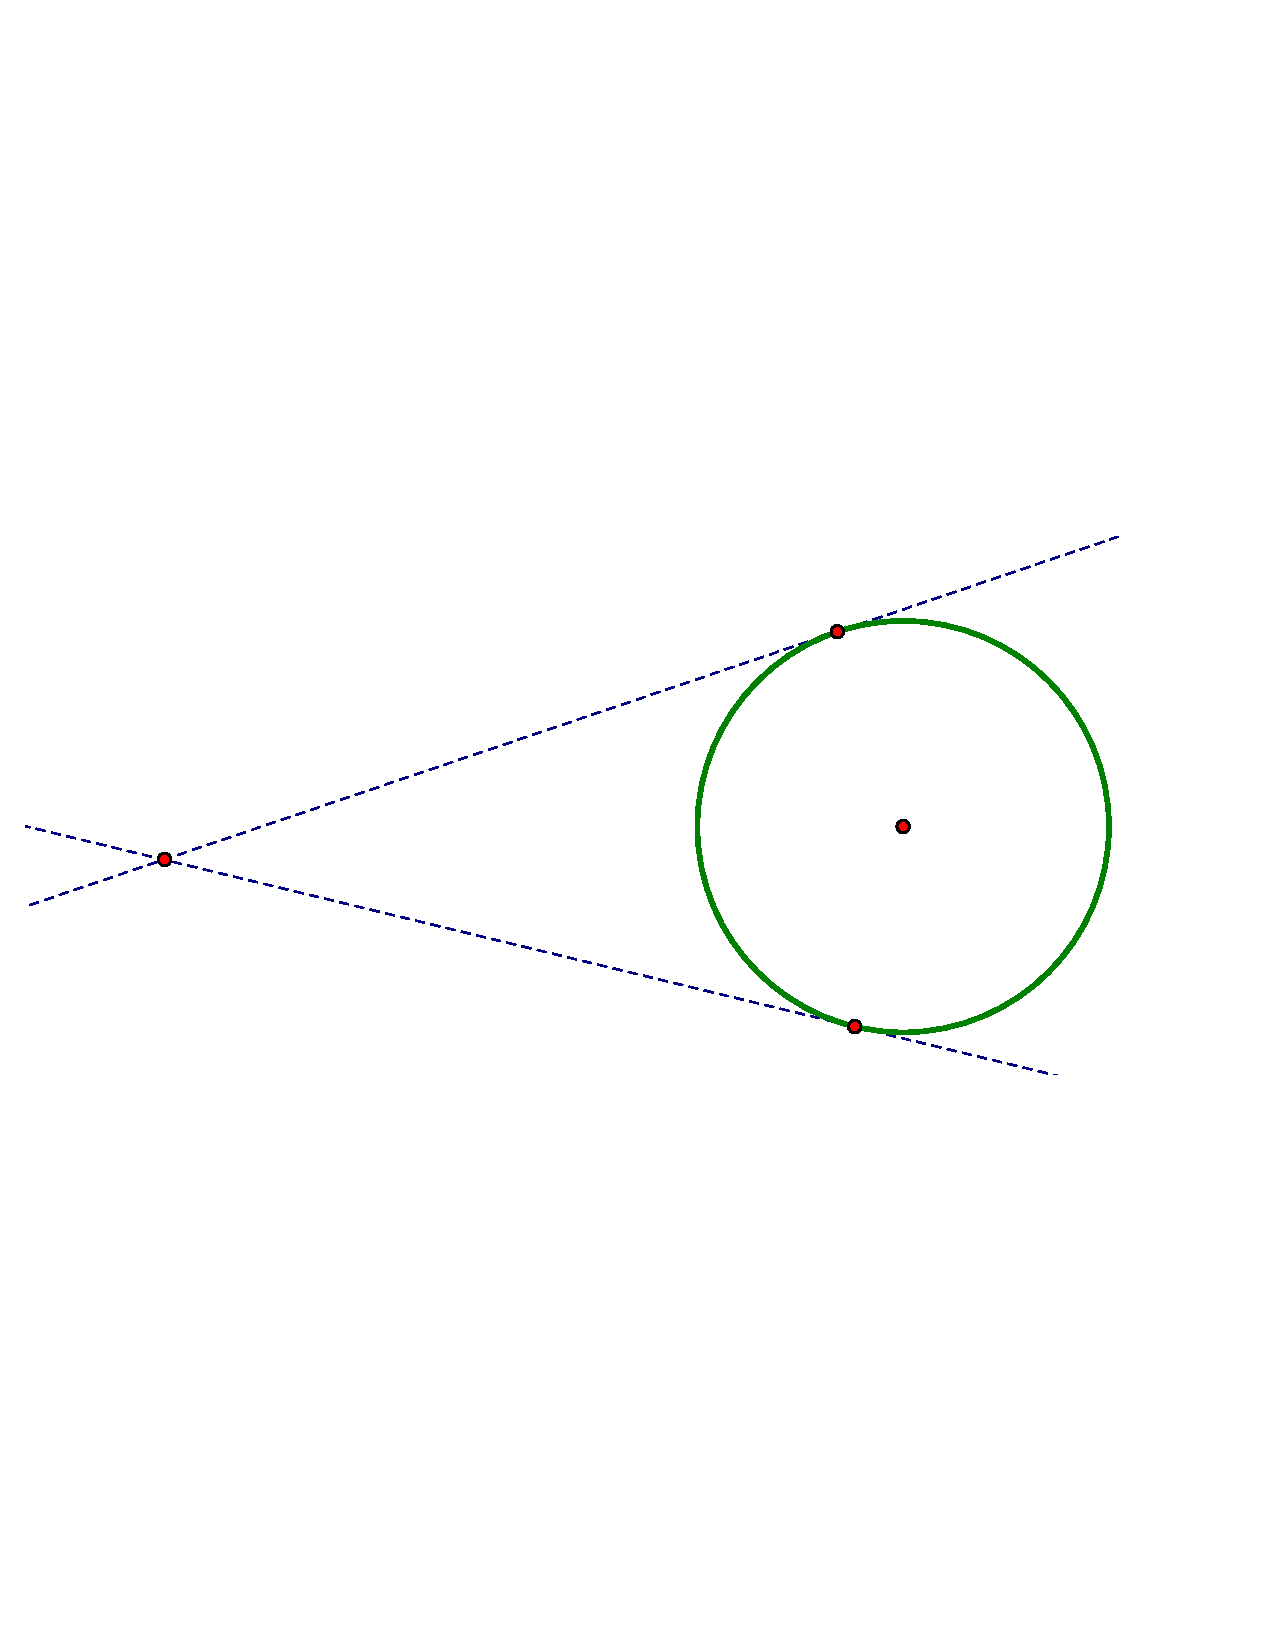
\includegraphics[scale=0.2]{tangent2.pdf}
%\end{image}
\begin{image}
\definecolor{qqqqff}{rgb}{0.,0.,1.}
\begin{tikzpicture}[scale=0.8,line cap=round,line join=round,>=triangle 45,x=1.0cm,y=1.0cm]
\clip(-9.0,-3.5) rectangle (4.1,3.5);
\draw [line width=0.7pt] (0.,0.) circle (3.cm);
\begin{scriptsize}
\draw [fill=qqqqff] (0.,0.) circle (1.5pt);
\draw [fill=qqqqff] (-8.,-1.) circle (1.5pt);
\end{scriptsize}
\end{tikzpicture}
\end{image}
\end{problem}

\newpage
\begin{problem}
Give an informal derivation of the relationship between the circumference and area of a circle.  Imagine cutting a circle into ``pie pieces'' and rearranging the pieces into a shape like the one below.  As the circle is cut into more and more equal-sized ``pie pieces,'' what does the rearranged shape begin to resemble?  Can you find the area of this shape?  
\begin{image}
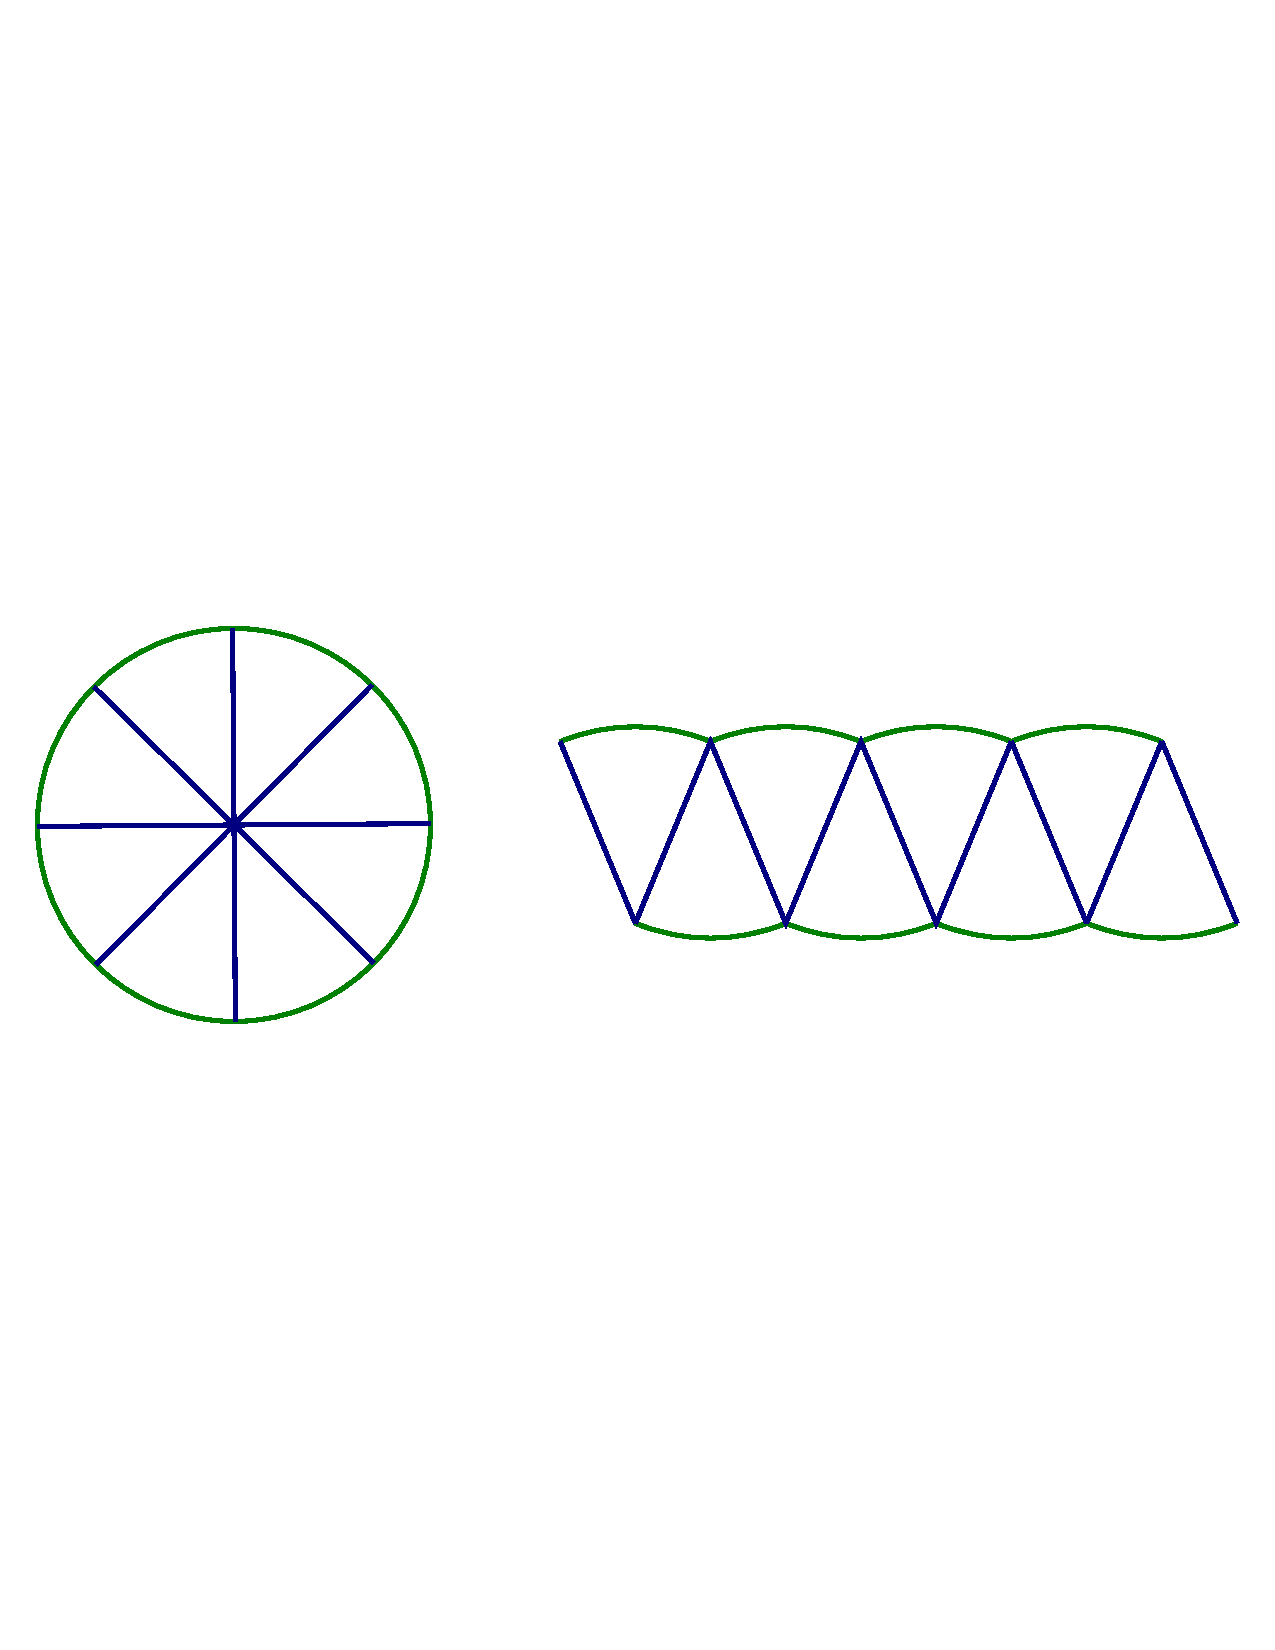
\includegraphics[width=3.5in]{circleArea.pdf}
\end{image}
\vfill
\end{problem}

\newpage
\begin{problem}
Derive a formula for the length of the arc intercepted by an central angle of a circle.  
\vfill
\end{problem}

\begin{problem}
Derive a formula for the area of a sector of a circle.  
\vfill
\end{problem}

%\begin{problem}
%Explain the following statement:  Given a central angle of a circle, the length of the intercepted arc is proportional to the radius of the circle.  The radian measure of the angle is the constant of proportionality.  (Hint:  Illustrate your explanation with a familiar angle.)
%\end{problem}
\end{document}

%\newpage

\section{Quadrilateral Diagonals}

Imagine you are working at a kite factory and you have been asked to design a new kite.  The kite will be a quadrilateral made of synthetic cloth, and it will be formed by two intersecting rods that serve as the diagonals of the quadrilateral and provide structure for the kite.  

\begin{prob}
To get started, review the definitions of all special quadrilaterals.  Be sure to include \emph{kite} on your list.  
\end{prob}

\begin{prob}
To consider the possible kite shapes, your first task is to describe how conditions on the diagonals determine the quadrilateral.  Use spaghetti to model the intersecting rods, and use paper and pencil to draw the rod configurations and resulting kite shapes.   Explore diagonals of various lengths, of the same length, and of different lengths.  Explore various places at which to attach the diagonals to each other, including at one or both of their midpoints.  Explore various angles that the diagonals might make with each other at their intersection, including the possibility of being perpendicular.  
\end{prob}

\begin{prob}
Summarize your findings in a table organized like the one below.  

\renewcommand\arraystretch{2}
\renewcommand\tabcolsep{6pt}
\begin{table}[h]
\begin{tabular}{|l|l|r|l|}
\hline
\multicolumn{1}{|c|}{\begin{tabular}[c]{@{}c@{}}Diagonal\\ Conditions\end{tabular}} & Quadrilateral & Definition & Other Key Properties \\ \hline
                                                                                    &               &            &                  \\ \hline
                                                                                    &               &            &                  \\ \hline
                                                                                    &               &            &                  \\ \hline
                                                                                    &               &            &                  \\ \hline
                                                                                    &               &            &                  \\ \hline
\end{tabular}
\end{table}

\end{prob}




 % old version
%\documentclass[handout]{ximera}
\documentclass[nooutcomes]{ximera}

\usepackage{gensymb}
\usepackage{tabularx}
\usepackage{mdframed}
\usepackage{pdfpages}
%\usepackage{chngcntr}

\let\problem\relax
\let\endproblem\relax

\newcommand{\property}[2]{#1#2}




\newtheoremstyle{SlantTheorem}{\topsep}{\fill}%%% space between body and thm
 {\slshape}                      %%% Thm body font
 {}                              %%% Indent amount (empty = no indent)
 {\bfseries\sffamily}            %%% Thm head font
 {}                              %%% Punctuation after thm head
 {3ex}                           %%% Space after thm head
 {\thmname{#1}\thmnumber{ #2}\thmnote{ \bfseries(#3)}} %%% Thm head spec
\theoremstyle{SlantTheorem}
\newtheorem{problem}{Problem}[]

%\counterwithin*{problem}{section}



%%%%%%%%%%%%%%%%%%%%%%%%%%%%Jenny's code%%%%%%%%%%%%%%%%%%%%

%%% Solution environment
%\newenvironment{solution}{
%\ifhandout\setbox0\vbox\bgroup\else
%\begin{trivlist}\item[\hskip \labelsep\small\itshape\bfseries Solution\hspace{2ex}]
%\par\noindent\upshape\small
%\fi}
%{\ifhandout\egroup\else
%\end{trivlist}
%\fi}
%
%
%%% instructorIntro environment
%\ifhandout
%\newenvironment{instructorIntro}[1][false]%
%{%
%\def\givenatend{\boolean{#1}}\ifthenelse{\boolean{#1}}{\begin{trivlist}\item}{\setbox0\vbox\bgroup}{}
%}
%{%
%\ifthenelse{\givenatend}{\end{trivlist}}{\egroup}{}
%}
%\else
%\newenvironment{instructorIntro}[1][false]%
%{%
%  \ifthenelse{\boolean{#1}}{\begin{trivlist}\item[\hskip \labelsep\bfseries Instructor Notes:\hspace{2ex}]}
%{\begin{trivlist}\item[\hskip \labelsep\bfseries Instructor Notes:\hspace{2ex}]}
%{}
%}
%% %% line at the bottom} 
%{\end{trivlist}\par\addvspace{.5ex}\nobreak\noindent\hung} 
%\fi
%
%


\let\instructorNotes\relax
\let\endinstructorNotes\relax
%%% instructorNotes environment
\ifhandout
\newenvironment{instructorNotes}[1][false]%
{%
\def\givenatend{\boolean{#1}}\ifthenelse{\boolean{#1}}{\begin{trivlist}\item}{\setbox0\vbox\bgroup}{}
}
{%
\ifthenelse{\givenatend}{\end{trivlist}}{\egroup}{}
}
\else
\newenvironment{instructorNotes}[1][false]%
{%
  \ifthenelse{\boolean{#1}}{\begin{trivlist}\item[\hskip \labelsep\bfseries {\Large Instructor Notes: \\} \hspace{\textwidth} ]}
{\begin{trivlist}\item[\hskip \labelsep\bfseries {\Large Instructor Notes: \\} \hspace{\textwidth} ]}
{}
}
{\end{trivlist}}
\fi


%% Suggested Timing
\newcommand{\timing}[1]{{\bf Suggested Timing: \hspace{2ex}} #1}




\hypersetup{
    colorlinks=true,       % false: boxed links; true: colored links
    linkcolor=blue,          % color of internal links (change box color with linkbordercolor)
    citecolor=green,        % color of links to bibliography
    filecolor=magenta,      % color of file links
    urlcolor=cyan           % color of external links
}

\title{Quadrilateral Diagonals}
\author{Bart Snapp and Brad Findell}

\outcome{Learning outcome goes here.}

\begin{document}
\begin{abstract}
  We explore basic shapes.
\end{abstract}
\maketitle 

\begin{teachingnote}
Supplies:  Fettuccini, scrap paper, 12-inch rulers.
\end{teachingnote}

Imagine you are working at a kite factory and you have been asked to design a new kite.  The kite will be a quadrilateral made of synthetic cloth, and it will be formed by two intersecting rods that serve as the diagonals of the quadrilateral and provide structure for the kite.  

\begin{problem}
To get started, review the definitions of all special quadrilaterals.  Be sure to include \emph{kite} on your list.  
\end{problem}

\begin{problem}
To consider the possible kite shapes, your task is to describe how conditions on the diagonals determine the quadrilateral.  Use fettuccine to model the intersecting rods, and use paper and pencil to draw the rod configurations and resulting kite shapes.  

Here are some hints:  

\begin{itemize}
\item Explore diagonals of various lengths, of the same length, and of different lengths.  
\item Explore various places at which to attach the diagonals to each other, including at one or both of their midpoints.  
\item Explore various angles that the diagonals might make with each other at their intersection, including the possibility of being perpendicular.  
\item Indicate what kinds of rotational or reflection symmetry you see in the resulting figure.
\end{itemize}
\end{problem}

\newpage
\begin{problem}
Summarize your findings in a table organized like the following.  
{
\renewcommand\arraystretch{2.8}
\renewcommand\tabcolsep{12pt}
\begin{table}[h]
\begin{tabular}{|l|p{4cm}|c|c|c|p{4cm}|}
\hline 
 & Definition  & \multicolumn{3}{c|}{Diagonals} &  Comments \\  %\hline
Quadrilateral & (A quad. with \dots) & \begin{sideways}Cong.\end{sideways} & 
\begin{sideways}Bisect\end{sideways} & \begin{sideways}Perp.\end{sideways} & (e.g., symmetry) \\ \hline\hline
Square           &            &   &  &         &                  \\  \hline
Rectangle       &           &   &  &         &                  \\ \hline
Rhombus        &           &   &  &         &                  \\ \hline
Parallelogram &           &   &  &         &                  \\ \hline
Kite                &           &   &  &          &                  \\ \hline
Trapezoid       &           &   &  &         &                  \\ \hline
Isosceles Trap.       &           &   &  &         &                  \\ \hline
\end{tabular}
\end{table}
}
\end{problem}



\end{document}


  

%\newpage
\section{I'm Into Triangles}

In this activity, we're going to see if we can discover a simple
method for breaking \textit{every} polygon into triangles.

\begin{prob}
Draw yourself a polygon with at least 8 sides. Show how to break this
polygon into triangles.
\end{prob}

\begin{prob}
See if you can figure out exactly \textbf{what} your method was for
breaking the polygon into triangles. Write it down. 
\end{prob}

\begin{prob}
Find a casual acquaintance and declare ``I challenge you to present me
with a polygon that cannot be broken into triangles.'' Can you use
your method to break their polygon into triangles?
\end{prob}

\begin{prob}
Draw a polygon that would be really difficult to break into triangles.
\end{prob}

\begin{prob}
Come up with a simple method that will \textbf{always} work for
breaking a polygon into triangles. As a hint, draw a stick person in
your polygon, and try to imagine what they see\dots
\end{prob}


   % How to cut a polygon into triangles:  Addressed in funkyShapes
%\newpage
\section{Morley's Miracle} %%remove * if added to notes!

Here is a construction that wasn't discovered until 1899. To make life
easier, I'm going to allow you to use the following (somewhat
imprecise) method for trisecting angles:

\begin{enumerate}
\item Fold the paper so that the crease leads up to the
  angle, with the edge of the flap being folded-over bisecting the
  new angle of the crease and the edge that was not moved.
\item Now fold the edge that was not moved on top of the flap that was
  just made. It should fit perfectly near the angle. If done
  correctly, the steps above should trisect the angle.
\end{enumerate}

\begin{prob}
What does that say above? I know, I know, it sounds complicated. See
if you can figure it out anyhow.
\end{prob}

So now get your tracing paper out, make a big scalene triangle, and
trisect all three angles.

\begin{prob}
Connect adjacent trisectors. Do you see a miracle happening? (I know, I
know, if \textit{anybody} can follow these directions than we truly
will have a miracle on our hands!)
\end{prob}
  

% Congruence and Similarity
%\documentclass[handout]{ximera}
\documentclass{ximera}

\usepackage{gensymb}
\usepackage{tabularx}
\usepackage{mdframed}
\usepackage{pdfpages}
%\usepackage{chngcntr}

\let\problem\relax
\let\endproblem\relax

\newcommand{\property}[2]{#1#2}




\newtheoremstyle{SlantTheorem}{\topsep}{\fill}%%% space between body and thm
 {\slshape}                      %%% Thm body font
 {}                              %%% Indent amount (empty = no indent)
 {\bfseries\sffamily}            %%% Thm head font
 {}                              %%% Punctuation after thm head
 {3ex}                           %%% Space after thm head
 {\thmname{#1}\thmnumber{ #2}\thmnote{ \bfseries(#3)}} %%% Thm head spec
\theoremstyle{SlantTheorem}
\newtheorem{problem}{Problem}[]

%\counterwithin*{problem}{section}



%%%%%%%%%%%%%%%%%%%%%%%%%%%%Jenny's code%%%%%%%%%%%%%%%%%%%%

%%% Solution environment
%\newenvironment{solution}{
%\ifhandout\setbox0\vbox\bgroup\else
%\begin{trivlist}\item[\hskip \labelsep\small\itshape\bfseries Solution\hspace{2ex}]
%\par\noindent\upshape\small
%\fi}
%{\ifhandout\egroup\else
%\end{trivlist}
%\fi}
%
%
%%% instructorIntro environment
%\ifhandout
%\newenvironment{instructorIntro}[1][false]%
%{%
%\def\givenatend{\boolean{#1}}\ifthenelse{\boolean{#1}}{\begin{trivlist}\item}{\setbox0\vbox\bgroup}{}
%}
%{%
%\ifthenelse{\givenatend}{\end{trivlist}}{\egroup}{}
%}
%\else
%\newenvironment{instructorIntro}[1][false]%
%{%
%  \ifthenelse{\boolean{#1}}{\begin{trivlist}\item[\hskip \labelsep\bfseries Instructor Notes:\hspace{2ex}]}
%{\begin{trivlist}\item[\hskip \labelsep\bfseries Instructor Notes:\hspace{2ex}]}
%{}
%}
%% %% line at the bottom} 
%{\end{trivlist}\par\addvspace{.5ex}\nobreak\noindent\hung} 
%\fi
%
%


\let\instructorNotes\relax
\let\endinstructorNotes\relax
%%% instructorNotes environment
\ifhandout
\newenvironment{instructorNotes}[1][false]%
{%
\def\givenatend{\boolean{#1}}\ifthenelse{\boolean{#1}}{\begin{trivlist}\item}{\setbox0\vbox\bgroup}{}
}
{%
\ifthenelse{\givenatend}{\end{trivlist}}{\egroup}{}
}
\else
\newenvironment{instructorNotes}[1][false]%
{%
  \ifthenelse{\boolean{#1}}{\begin{trivlist}\item[\hskip \labelsep\bfseries {\Large Instructor Notes: \\} \hspace{\textwidth} ]}
{\begin{trivlist}\item[\hskip \labelsep\bfseries {\Large Instructor Notes: \\} \hspace{\textwidth} ]}
{}
}
{\end{trivlist}}
\fi


%% Suggested Timing
\newcommand{\timing}[1]{{\bf Suggested Timing: \hspace{2ex}} #1}




\hypersetup{
    colorlinks=true,       % false: boxed links; true: colored links
    linkcolor=blue,          % color of internal links (change box color with linkbordercolor)
    citecolor=green,        % color of links to bibliography
    filecolor=magenta,      % color of file links
    urlcolor=cyan           % color of external links
}

\title{Congruence via Transformations}
\author{Bart Snapp and Brad Findell}

\outcome{Learning outcome goes here.}

\begin{document}
\begin{abstract}
Abstract goes here.  
\end{abstract}
\maketitle

\begin{teachingnote}
Supplies:  Tracing paper, long rulers for drawing these on the board.  
\end{teachingnote}

Informally, a \emph{transformation} of the plane is a ``motion,'' such as a rotation or a stretch of the plane, that takes a figure to an \emph{image} of that figure.  This activity explores the basic rigid motions: translations (slides), rotations (turns), and reflections (flips).  


\begin{problem}
One of the pairs of figures below shows a translation, and the other pair does not.  To identify which is which, draw segments between each point and its image.  Use those segments to explain your reasoning.
\begin{image}
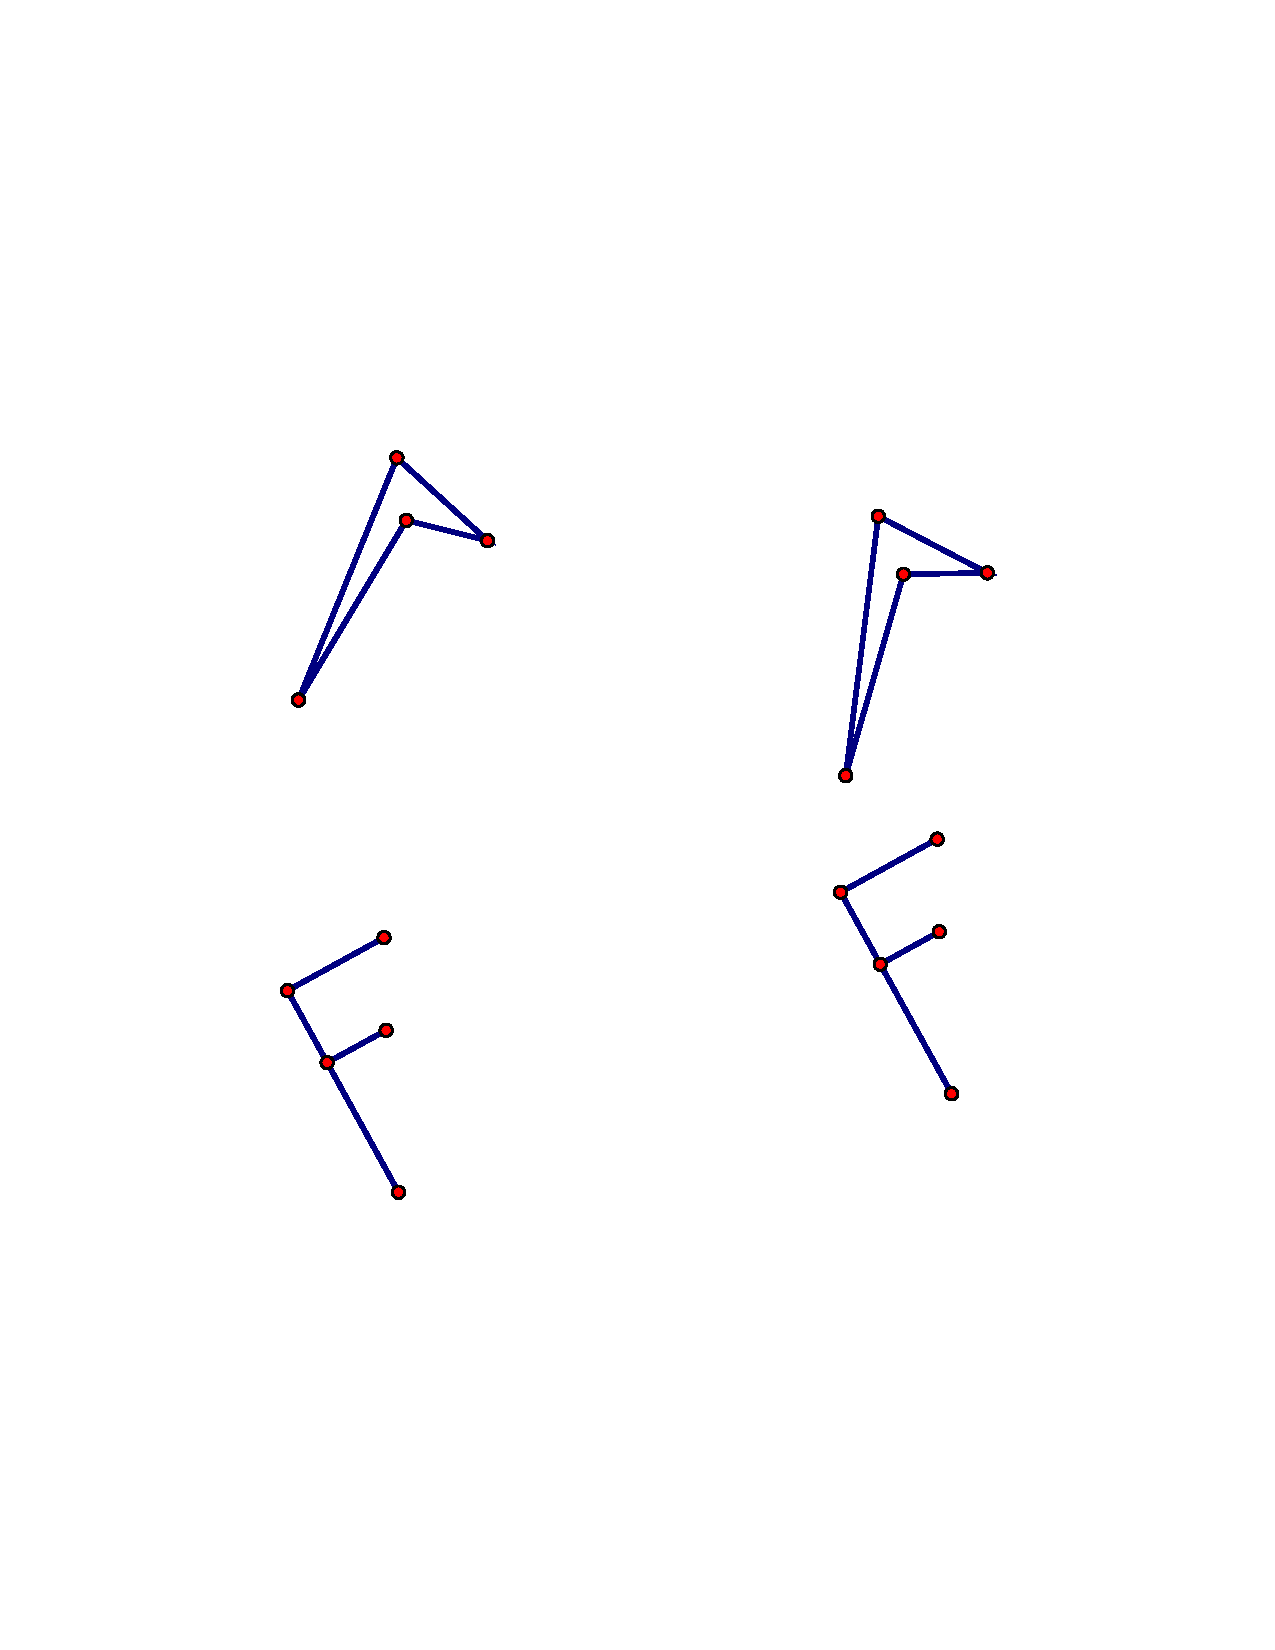
\includegraphics[scale=0.8]{translate.pdf}
\end{image}
\end{problem}

\newpage
\begin{problem}
One of the pairs of figures shows a reflection about the given line, and the other pair does not.  
\begin{enumerate}
\item Identify which pair of figures shows a reflection about the given line, and explain how you know. 
\item Find the line of reflection for the other pair of figures, and explain your reasoning.  
\begin{image}
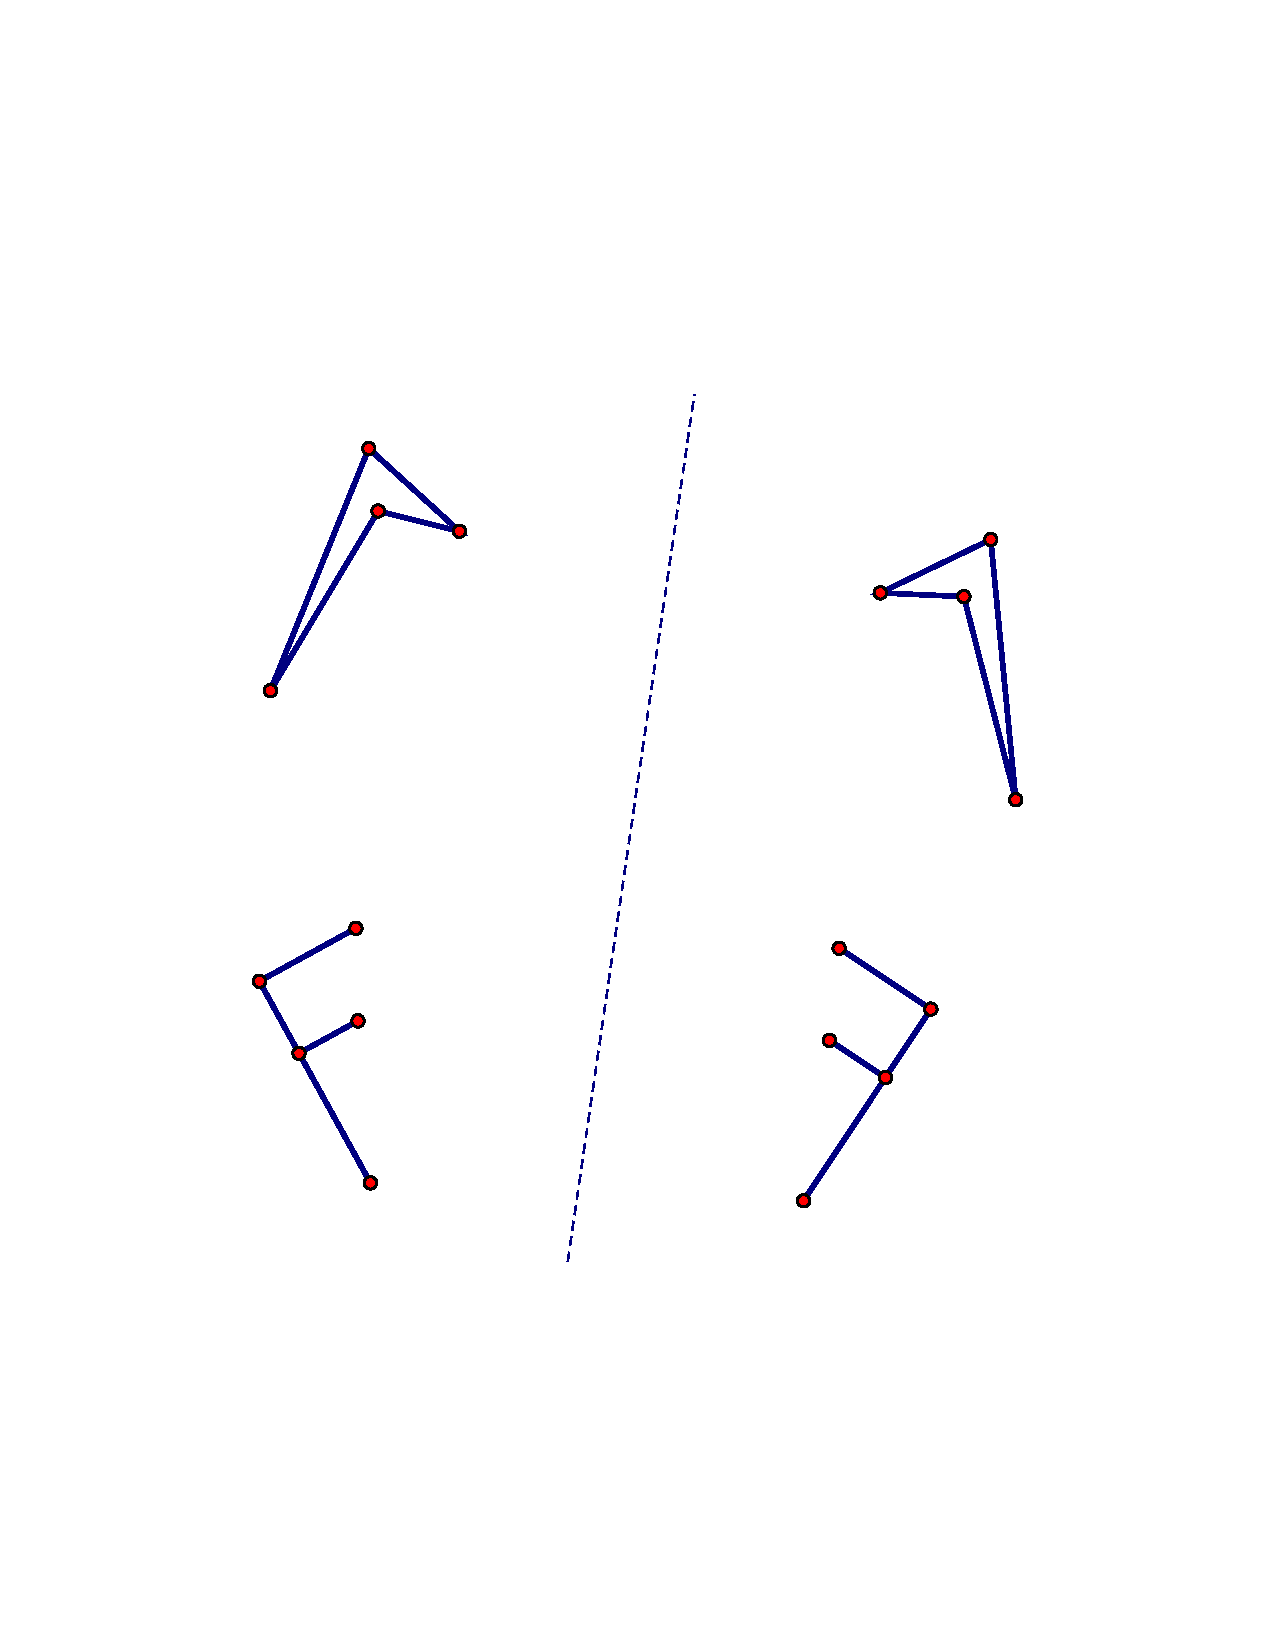
\includegraphics[scale=0.8]{reflect.pdf}
\end{image}
\end{enumerate}
\end{problem}

\newpage
\begin{problem}
One of the pairs of figures below shows a rotation about point $C$, and the other pair does not. 
\begin{enumerate}
\item Identify which pair of figures shows a rotation about $C$, and explain how you know.  
\item Find the angle of rotation.  
\item Find the center of and angle of rotation for the other pair of figures.  Explain your reasoning.  
\begin{image}
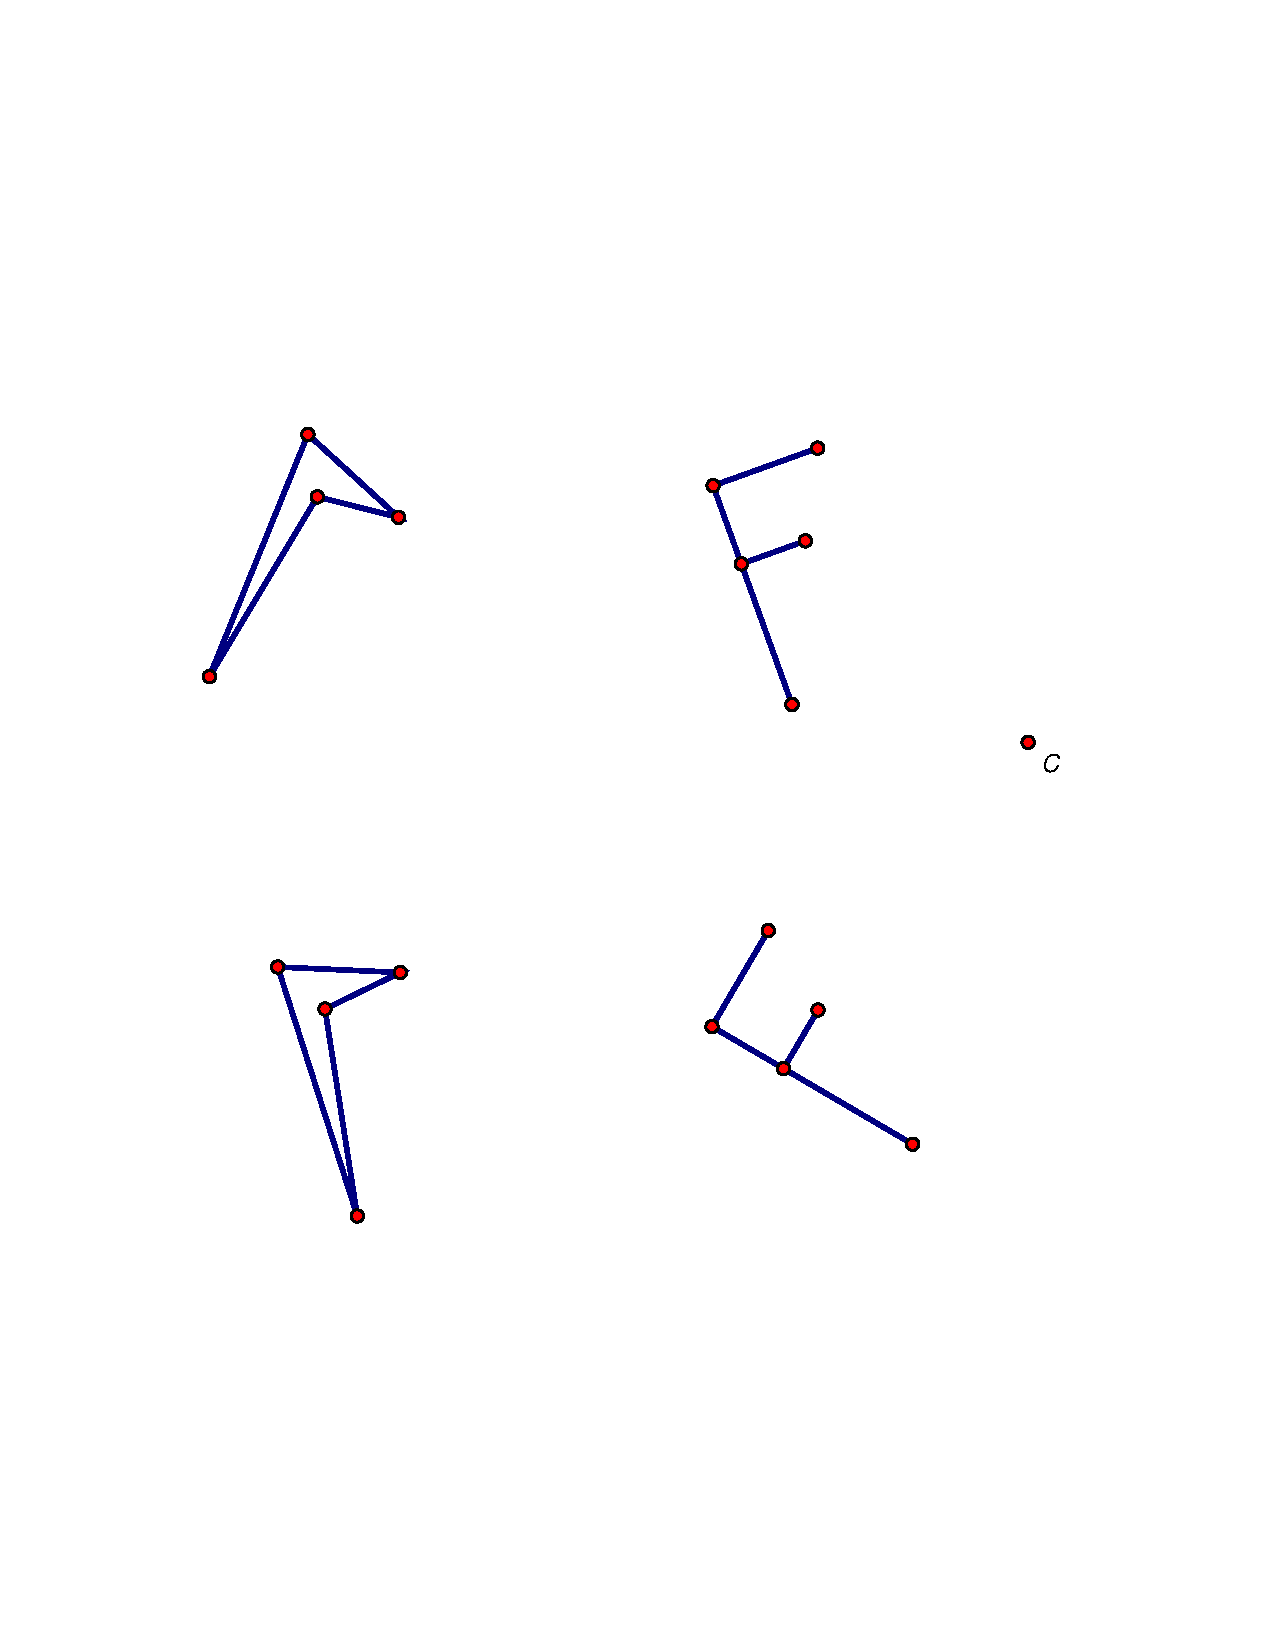
\includegraphics[scale=0.8]{../graphics/rotate.pdf}
\end{image}
\end{enumerate}
\end{problem}


\newpage
\begin{problem}
Two figures are said to be \emph{congruent} if there is a sequence of basic rigid motions that take one figure onto the other.  
\begin{enumerate}
\item Specify a sequence of two or three basic rigid motions that takes one F onto the other.  Illustrate intermediate images.  Explain your reasoning.  
\vspace{1in}
\begin{image}
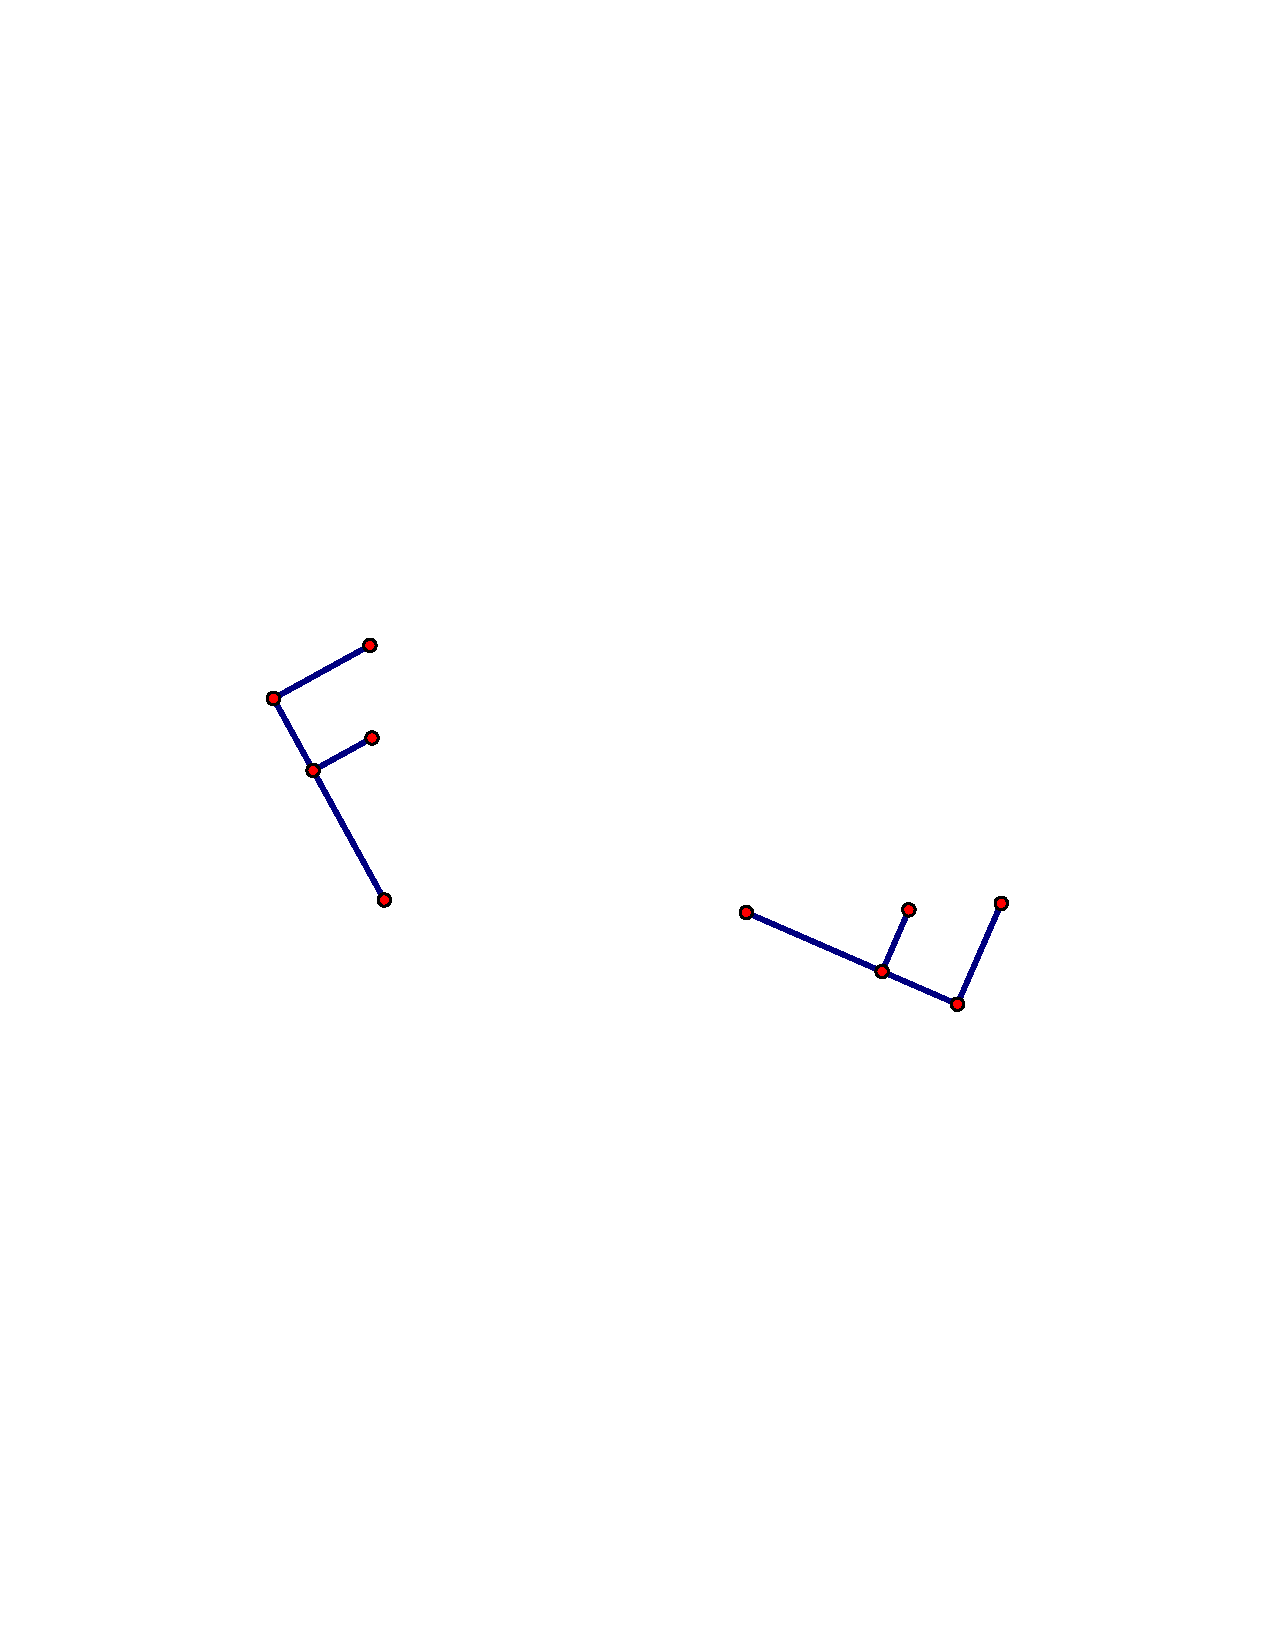
\includegraphics[scale=0.8]{../graphics/glideReflect.pdf}
\end{image}
\vspace{0.5in}
\item Explain briefly why, for this pair of figures, sequences of the following types cannot work: 
\begin{itemize}
\item a rotation followed by a rotation
\item a translation followed by a translation
\item a reflection followed by a reflection
\end{itemize}
\end{enumerate}
\end{problem}
\end{document}

\newpage

\section{More Transformations}
\begin{teachingnote}
Supplies:  tracing paper.  Helpful to label the vertices and pay attention to where they go in the symmetry transformation.  The named lines of symmetry don't move when the figure moves.
\end{teachingnote}

Transformations of the plane are considered to be functions that take points as inputs and produce 
points as outputs.  Given a point as input, the corresponding output value is often called 
the \emph{image} of the point under the transformation.\standardhs{G-CO.2}
\begin{prob}
Based on your experience with the basic rigid motions, write definitions of translation, rotation, and reflection.\standardhs{G-CO.4} For each definition, be sure to indicate (1) what it takes to specify the transformation, and (2) how to produce the image of a given point.  
\begin{enumerate}
\item Translation: 
\vspace{0.3in}
\item Rotation: 
\vspace{0.3in}
\item Reflection: 
\vspace{0.3in}
\end{enumerate}
\end{prob}

\begin{prob}
Now explore sequences of basic rigid motions.  Here are some suggestions to support your explorations:  
\begin{itemize}\itemsep0pt
\item Use a non-symmetric figure (such as an F). 
\item Use one sheet of tracing paper as the original plane, and use a second sheet of paper to carry out the sequence of transformations.  
\item Trace intermediate figures on both sheets of paper, to keep track of the work.   
\item For reflections, trace the line of reflection on both sheets. 
\item For rotations, use a protractor to help you keep track of angles.  
\item Consider special cases, such as reflections about the same line or rotations about the same point.  
\item Try to predict the result before you actually carry out the sequence of transformations.  
\end{itemize}
Describe briefly what you can say about each of the following sequences of basic rigid motions.  Include special cases in your descriptions.  
\begin{enumerate}
\item Translation followed by translation
\vspace{0.5in}
\item Rotation followed by rotation
\vspace{0.5in}
\item Reflection followed by reflection
\vspace{0.5in}
\item Translation followed by rotation
\vspace{0.5in}
\item Translation followed by reflection
\vspace{0.5in}
\item Rotation followed by reflection
\end{enumerate}
\end{prob}


%\documentclass[handout]{ximera}
\documentclass[nooutcomes]{ximera}

\usepackage{gensymb}
\usepackage{tabularx}
\usepackage{mdframed}
\usepackage{pdfpages}
%\usepackage{chngcntr}

\let\problem\relax
\let\endproblem\relax

\newcommand{\property}[2]{#1#2}




\newtheoremstyle{SlantTheorem}{\topsep}{\fill}%%% space between body and thm
 {\slshape}                      %%% Thm body font
 {}                              %%% Indent amount (empty = no indent)
 {\bfseries\sffamily}            %%% Thm head font
 {}                              %%% Punctuation after thm head
 {3ex}                           %%% Space after thm head
 {\thmname{#1}\thmnumber{ #2}\thmnote{ \bfseries(#3)}} %%% Thm head spec
\theoremstyle{SlantTheorem}
\newtheorem{problem}{Problem}[]

%\counterwithin*{problem}{section}



%%%%%%%%%%%%%%%%%%%%%%%%%%%%Jenny's code%%%%%%%%%%%%%%%%%%%%

%%% Solution environment
%\newenvironment{solution}{
%\ifhandout\setbox0\vbox\bgroup\else
%\begin{trivlist}\item[\hskip \labelsep\small\itshape\bfseries Solution\hspace{2ex}]
%\par\noindent\upshape\small
%\fi}
%{\ifhandout\egroup\else
%\end{trivlist}
%\fi}
%
%
%%% instructorIntro environment
%\ifhandout
%\newenvironment{instructorIntro}[1][false]%
%{%
%\def\givenatend{\boolean{#1}}\ifthenelse{\boolean{#1}}{\begin{trivlist}\item}{\setbox0\vbox\bgroup}{}
%}
%{%
%\ifthenelse{\givenatend}{\end{trivlist}}{\egroup}{}
%}
%\else
%\newenvironment{instructorIntro}[1][false]%
%{%
%  \ifthenelse{\boolean{#1}}{\begin{trivlist}\item[\hskip \labelsep\bfseries Instructor Notes:\hspace{2ex}]}
%{\begin{trivlist}\item[\hskip \labelsep\bfseries Instructor Notes:\hspace{2ex}]}
%{}
%}
%% %% line at the bottom} 
%{\end{trivlist}\par\addvspace{.5ex}\nobreak\noindent\hung} 
%\fi
%
%


\let\instructorNotes\relax
\let\endinstructorNotes\relax
%%% instructorNotes environment
\ifhandout
\newenvironment{instructorNotes}[1][false]%
{%
\def\givenatend{\boolean{#1}}\ifthenelse{\boolean{#1}}{\begin{trivlist}\item}{\setbox0\vbox\bgroup}{}
}
{%
\ifthenelse{\givenatend}{\end{trivlist}}{\egroup}{}
}
\else
\newenvironment{instructorNotes}[1][false]%
{%
  \ifthenelse{\boolean{#1}}{\begin{trivlist}\item[\hskip \labelsep\bfseries {\Large Instructor Notes: \\} \hspace{\textwidth} ]}
{\begin{trivlist}\item[\hskip \labelsep\bfseries {\Large Instructor Notes: \\} \hspace{\textwidth} ]}
{}
}
{\end{trivlist}}
\fi


%% Suggested Timing
\newcommand{\timing}[1]{{\bf Suggested Timing: \hspace{2ex}} #1}




\hypersetup{
    colorlinks=true,       % false: boxed links; true: colored links
    linkcolor=blue,          % color of internal links (change box color with linkbordercolor)
    citecolor=green,        % color of links to bibliography
    filecolor=magenta,      % color of file links
    urlcolor=cyan           % color of external links
}

\title{Symmetries}
\author{Bart Snapp and Brad Findell}

\outcome{Learning outcome goes here.}

\begin{document}
\begin{abstract}
  We introduce symmetries.
\end{abstract}
\maketitle

\begin{teachingnote}
\end{teachingnote}

\begin{definition}
A symmetry is a transformation that takes a figure onto itself.  
\end{definition}
\begin{problem}
List the symmetries of an equilateral triangle.  Explain how you know you have them all.  
\end{problem}

\begin{problem}
Flip through these notes and describe the symmetries you notice.  Try to find reflection symmetry, rotation symmetry, and translation symmetry.  
\end{problem}

\begin{teachingnote}
To augment the examples, bring some pictures from Web.   Tesselations and Frieze patterns are necessary for translation symmetry.  
\end{teachingnote}

\begin{problem}
Suppose the symmetries of a square are called $R_0$, $R_{90}$, $R_{180}$, $R_{270}$, $V$, $H$, $D$, $D'$, based upon the figure below.  
\begin{image}
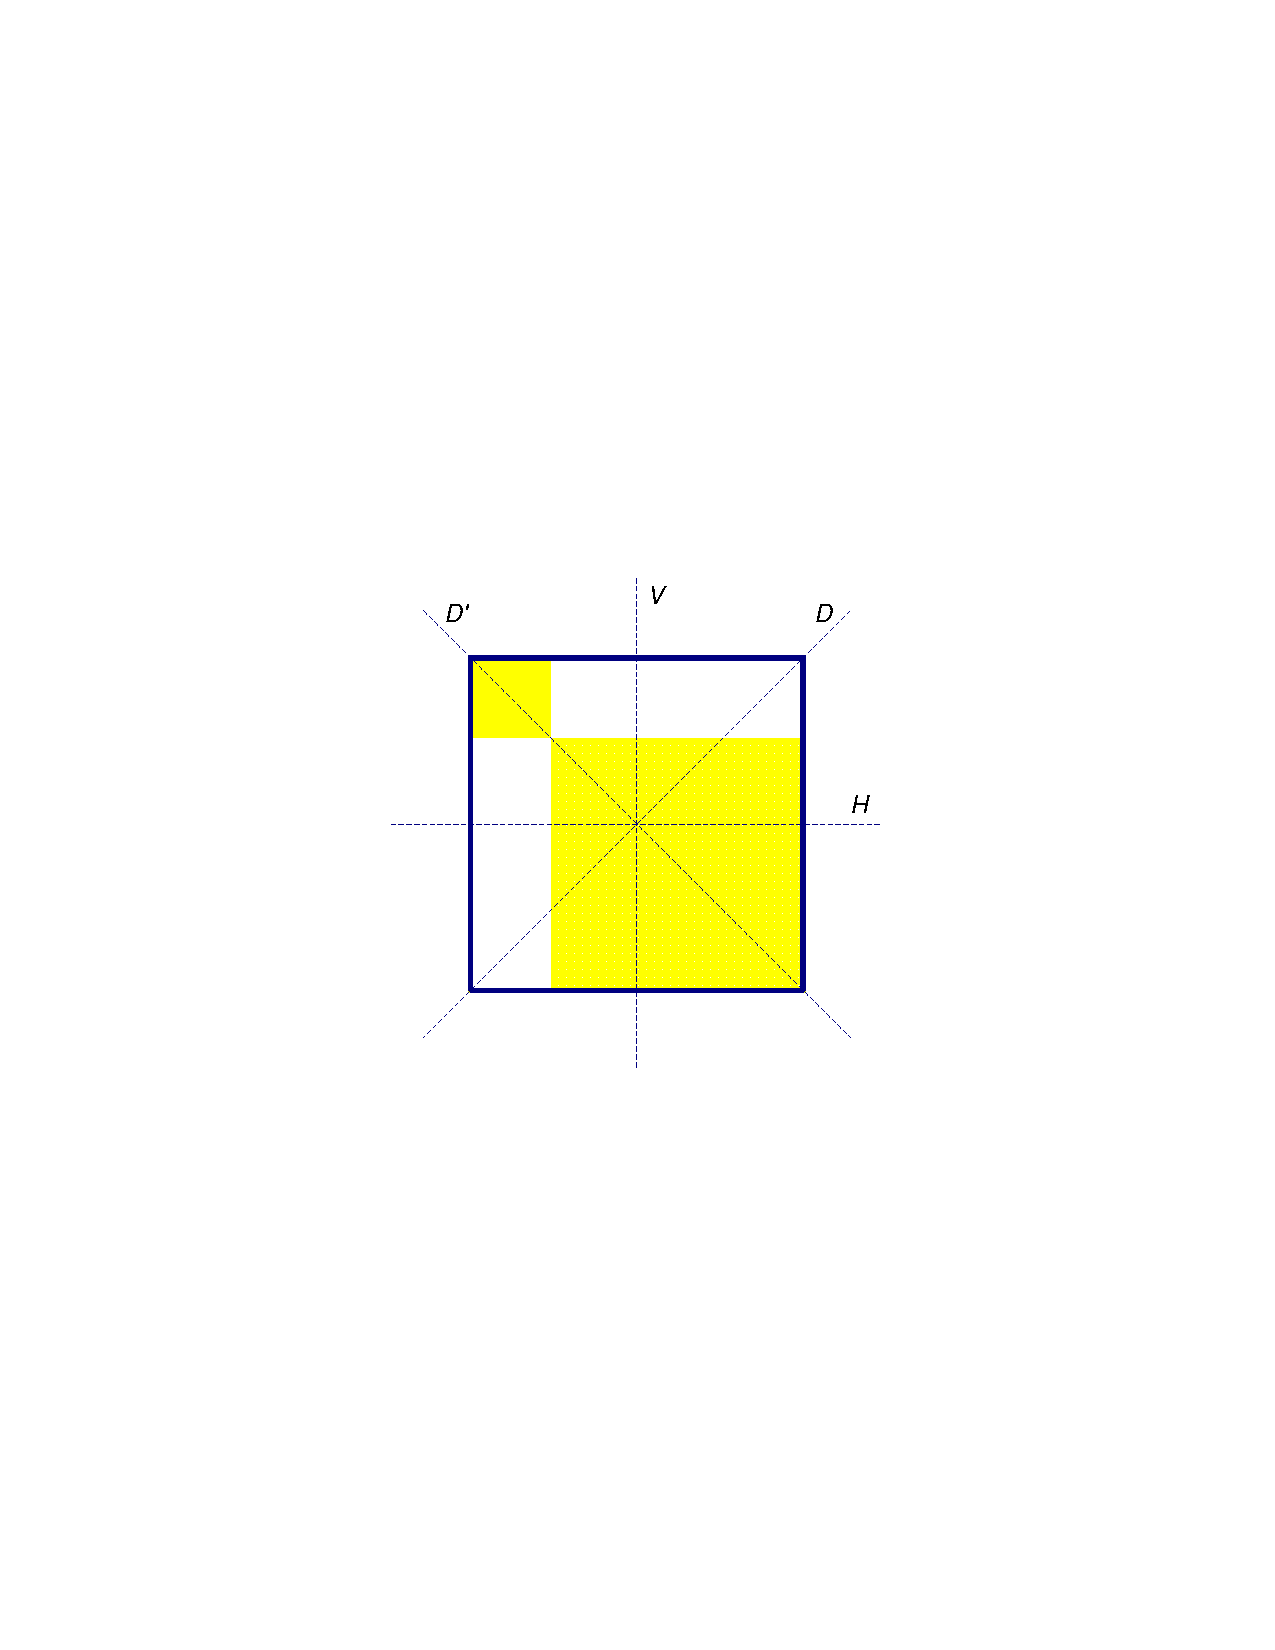
\includegraphics[scale=0.6]{D4.pdf}
\end{image}
Hint:  To identify a single transformation that accomplishes a sequence of transformations, do the transformations physically with a square piece of paper marked with ``FRONT'' on the side that starts facing you.  Or mark the corners of the square with $A$, $B$, $C$, and $D$.  
\begin{enumerate}
\item Complete the following table, where the entry at (row, column) is the symmetry that results from the sequence of symmetries given by the row heading followed by the column heading.  
\item What patterns and not-quite-patterns do you notice in the table?  For example, which elements ``commute'' with which other elements?
\item What facts about isometries can you observe in the table?  For example, what can you say generally about sequences of rotations and reflections?  
\end{enumerate}
\[
{\arraycolsep=12pt\def\arraystretch{3}
\begin{array}{|l||l|l|l|l||l|l|l|l|}
\hline
 & R_0 & R_{90} & R_{180} & R_{270} & V & H & D & D' \\ \hline\hline
R_0 & & & & & & & & \\ \hline
R_{90} & & & & & & & & \\ \hline
R_{180} & & & & & & & & \\ \hline
R_{270} & & & & & & & & \\ \hline\hline
V & & & & & & & & \\ \hline
H & & & & & & & & \\ \hline
D & & & & & & & & \\ \hline
D' & & & & & & & & \\ \hline
\end{array}
}\]
\end{problem}

\begin{teachingnote}
Blurring one's eyes, it is possible to notice (1) the composition of a reflection and a rotation (in either order) is a reflection; (2) the composition of two rotations is a rotation; and (3) the composition of two reflections is a rotation.  Looking a bit closer, one can see that some elements commute with one another and others do not.  
\end{teachingnote}
\end{document}

\newpage

\section{Congruence Criteria}
\begin{teachingnote}
Perhaps ask students to come up with the sequence of transformations. 

Discuss a common error:   Translate $\triangle ABC$ through the vector $\overrightarrow{BY}$.  Then rotate about $Y$ by $\angle C'YZ.$. 

The generality of the proofs requires consideration of the possibility that a reflection might not be necessary in the general case.  Use half-plane ideas to ask whether points are on the same side or opposite sides of lines.  

Simplify by eliminating the prime notation.  After the translation, for example, $A$ coincides with $X$.  (See photos from class.)
\end{teachingnote}

In this activity, we show how the common triangle congruence criteria follow from
 what we now know about isometries.\standardhs{G-CO.8}  Recall that two figures are said to be 
congruent if there exists an isometry (translation, rotation, or reflection) or a 
sequence of isometries that maps one figure onto the other.  

\begin{prob}
Proof of Side-Angle-Side (SAS) congruence.  Suppose $\triangle ABC$ and $\triangle XYZ$ are such that $AB=XY$, $AC=XZ$, and $\angle A \cong \angle X$.  Prove, using basic rigid motions, that $\triangle ABC \cong \triangle XYZ$.  Consider the figure below.  
$$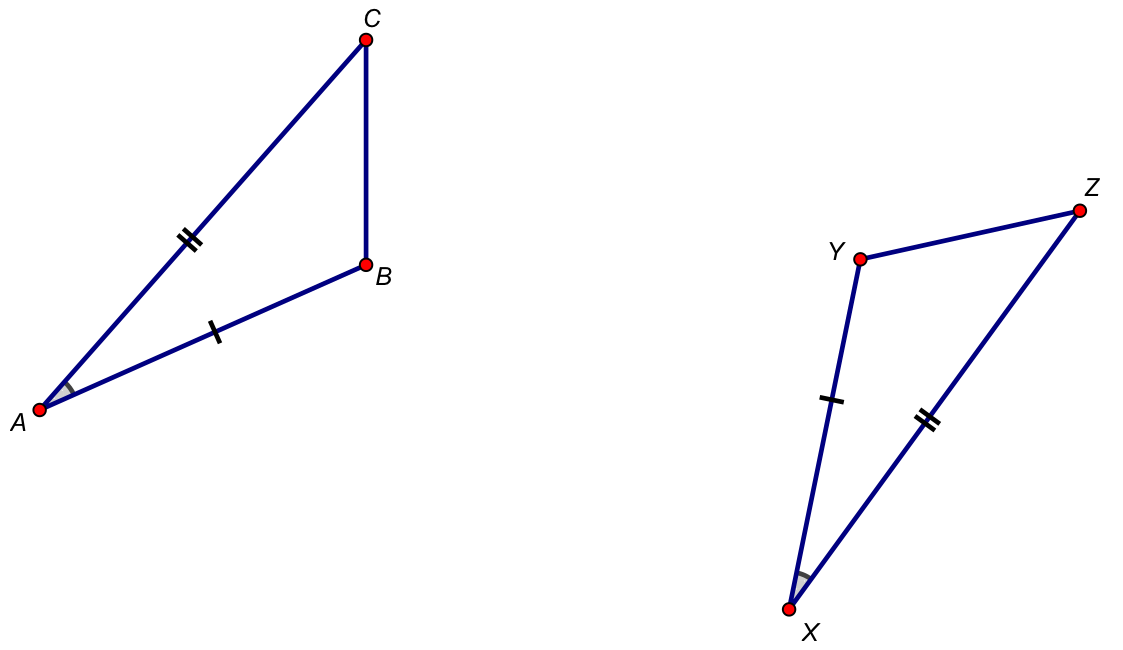
\includegraphics[scale=0.6]{../graphics/SAS}$$
Fill in the details of the following proof.  
\begin{enumerate}
\item Translate $\triangle ABC$ through the vector $\overrightarrow{AX}$.  Call the image $\triangle A'B'C'$.  Explain why $A'$ and $X$ coincide.
\item Rotate $\triangle A'B'C'$ about $X=A'$ through $\angle B'XY$ so that ray $\overrightarrow{A'B'}$ is along ray $\overrightarrow{XY}$.  Call the image $\triangle A''B''C''$   Explain how you know the segments $\overline{A''B''}$ and $\overline{XY}$ coincide. 
\item Reflect $\triangle A''B''C''$ about the line $\overleftrightarrow{A''B''} = \overleftrightarrow{XY}$.  Call the image $\triangle A'''B'''C'''$.  Explain why $\overline{A'''C'''}$ and $\overline{XZ}$ coincide.
\item Explain how you now know that all sides and angles of $\triangle A'''B'''C'''$ are congruent to the corresponding sides and angles of $\triangle XYZ$.  
\item Explain how to modify the above steps to handle the following different cases: 
\begin{itemize}
\item Initially $X = A$. 
\item After the translation, $\overline{A'B'}$ and $\overline{XY}$ coincide. 
\item After the rotation, $\overline{A''C''}$ and $\overline{XZ}$ coincide.  (Hint:  Consider whether $C''$ and $Z$ are on the same side or on opposite sides of $\overleftrightarrow{XZ}$.)  
\end{itemize}
\end{enumerate}
\end{prob}

\begin{prob}
Proof of Angle-Side-Angle (ASA) congruence.  Suppose $\triangle ABC$ and $\triangle XYZ$ are such that $AB=XY$, $\angle A \cong \angle X$, and $\angle B \cong \angle Y$.  Prove, using basic rigid motions, that $\triangle ABC \cong \triangle XYZ$.  
\begin{enumerate}
\item Outline a general proof for the figure below.  
$$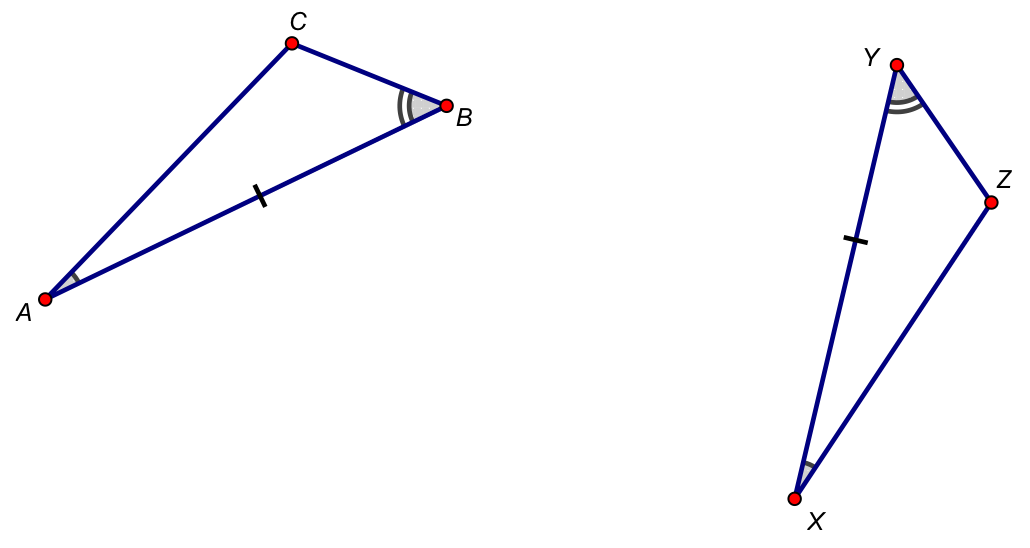
\includegraphics[scale=0.6]{../graphics/ASA}$$
\item Explain carefully how you know, after the sequence of rigid motions, that the ``final image'' of $C$ coincides with $Z$.  
\item Describe how to modify the outline to handle other cases. 
\end{enumerate}
\end{prob}

\begin{prob}
In a previous activity, you used triangle congruence criteria to prove the following results: 
\begin{itemize}
\item The Isosceles Triangle Theorem.
\item The points on a perpendicular bisector of a segment are exactly those that are equidistant from the endpoints.
\end{itemize}
Verify that these results could have been established using only SAS and ASA congruence.  (Thus, you may use these results in the problems that follow.) 
\end{prob}

\begin{prob}
Proof of Hypotenuse-Leg (HL) congruence.  Suppose $\triangle ABC$ and $\triangle XYZ$ are such that $\angle C$ and $\angle Z$ are right angles, $AB=XY$, and $BC=YZ$.  Prove that $\triangle ABC \cong \triangle XYZ$.  
$$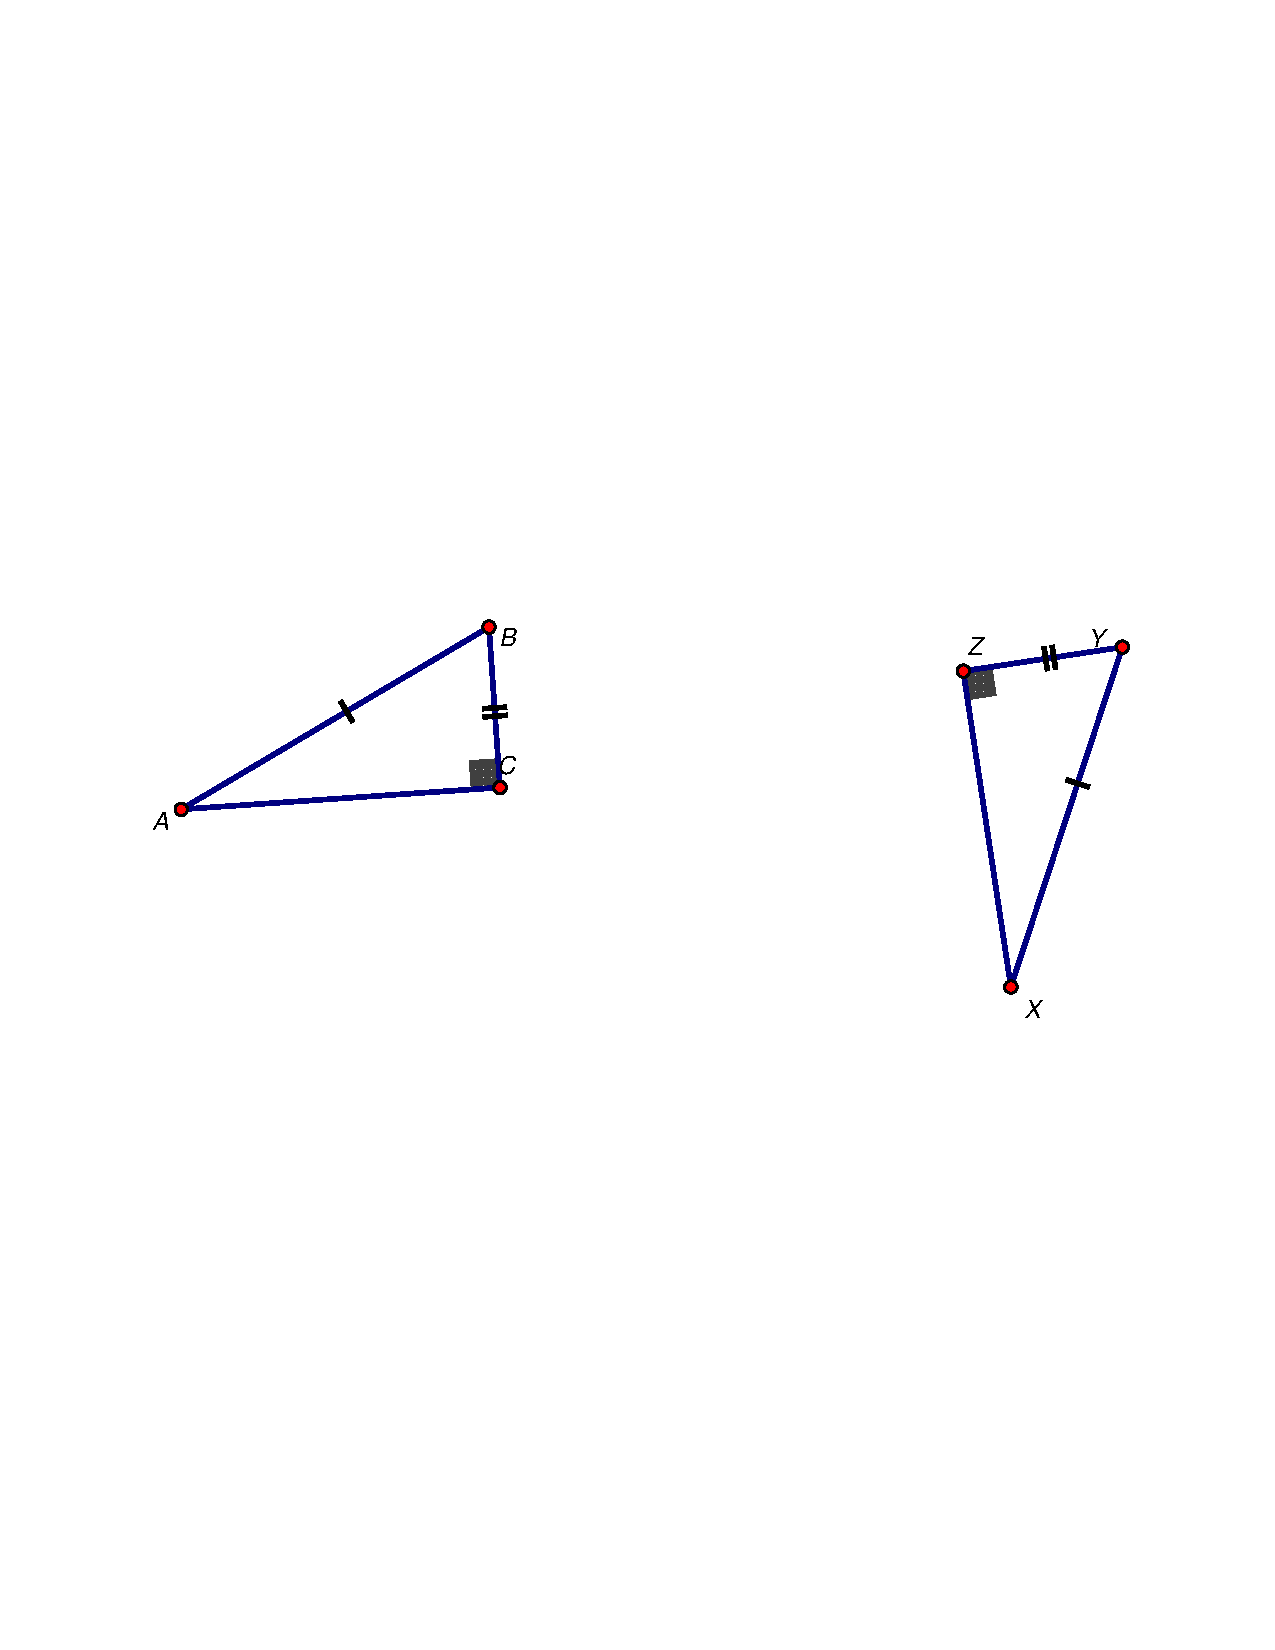
\includegraphics[scale=0.6]{../graphics/HL}$$
\end{prob}

\begin{teachingnote}
One approach:  First extend side $\overrightarrow{AC}$ to a point $A'$ so that $CA'=XZ$, and argue that $\triangle A'BC \cong \triangle XYZ$.

Easier:  Translate $\triangle ABC$ through the vector $\overrightarrow{CZ}$.  Then rotate.

Alternatively, save HL until after SSS?
\end{teachingnote}


\begin{prob}
Proof of Side-Side-Side (SSS) congruence.  Suppose $\triangle ABC$ and $\triangle XYZ$ are such that $AB=XY$, $AC=XZ$, and $BC=YZ$.  Prove, using basic rigid motions, that $\triangle ABC \cong \triangle XYZ$.  Build toward the general case through the following steps:  
\begin{teachingnote}
Or maybe these two figures don't matter if we emphasize that $A$ and $B$ both lie on the perpendicular bisector of $\overline{CZ}$.
\end{teachingnote}
\begin{enumerate}
\item Case 1a:  $A=X$, $B=Y$, and $C$ and $Z$ lie on opposite sides of $\overleftrightarrow{AB}$.  (Hint:  Explain why the situation must be like one of the figures below, argue that $\overleftrightarrow{AB}$ is the perpendicular bisector of $\overline{CZ}$, and then use a reflection.)
$$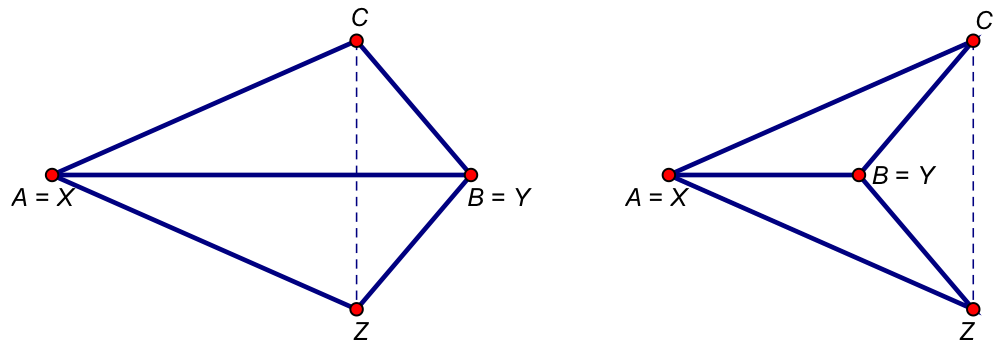
\includegraphics[scale=0.6]{../graphics/SSS}$$
\item Case 1b:  $A=X$, $B=Y$, and $C$ and $Z$ lie on the same side of $\overleftrightarrow{AB}=\overleftrightarrow{XY}$.  (Hint: Consider a reflection of one of the triangles and use the previous case.)  
\item Case 2:  $A=X$ but $B \ne Y$.
\item Case 3: The general case.  
\end{enumerate}
\end{prob}




%\documentclass[handout]{ximera}
\documentclass[nooutcomes]{ximera}

\usepackage{gensymb}
\usepackage{tabularx}
\usepackage{mdframed}
\usepackage{pdfpages}
%\usepackage{chngcntr}

\let\problem\relax
\let\endproblem\relax

\newcommand{\property}[2]{#1#2}




\newtheoremstyle{SlantTheorem}{\topsep}{\fill}%%% space between body and thm
 {\slshape}                      %%% Thm body font
 {}                              %%% Indent amount (empty = no indent)
 {\bfseries\sffamily}            %%% Thm head font
 {}                              %%% Punctuation after thm head
 {3ex}                           %%% Space after thm head
 {\thmname{#1}\thmnumber{ #2}\thmnote{ \bfseries(#3)}} %%% Thm head spec
\theoremstyle{SlantTheorem}
\newtheorem{problem}{Problem}[]

%\counterwithin*{problem}{section}



%%%%%%%%%%%%%%%%%%%%%%%%%%%%Jenny's code%%%%%%%%%%%%%%%%%%%%

%%% Solution environment
%\newenvironment{solution}{
%\ifhandout\setbox0\vbox\bgroup\else
%\begin{trivlist}\item[\hskip \labelsep\small\itshape\bfseries Solution\hspace{2ex}]
%\par\noindent\upshape\small
%\fi}
%{\ifhandout\egroup\else
%\end{trivlist}
%\fi}
%
%
%%% instructorIntro environment
%\ifhandout
%\newenvironment{instructorIntro}[1][false]%
%{%
%\def\givenatend{\boolean{#1}}\ifthenelse{\boolean{#1}}{\begin{trivlist}\item}{\setbox0\vbox\bgroup}{}
%}
%{%
%\ifthenelse{\givenatend}{\end{trivlist}}{\egroup}{}
%}
%\else
%\newenvironment{instructorIntro}[1][false]%
%{%
%  \ifthenelse{\boolean{#1}}{\begin{trivlist}\item[\hskip \labelsep\bfseries Instructor Notes:\hspace{2ex}]}
%{\begin{trivlist}\item[\hskip \labelsep\bfseries Instructor Notes:\hspace{2ex}]}
%{}
%}
%% %% line at the bottom} 
%{\end{trivlist}\par\addvspace{.5ex}\nobreak\noindent\hung} 
%\fi
%
%


\let\instructorNotes\relax
\let\endinstructorNotes\relax
%%% instructorNotes environment
\ifhandout
\newenvironment{instructorNotes}[1][false]%
{%
\def\givenatend{\boolean{#1}}\ifthenelse{\boolean{#1}}{\begin{trivlist}\item}{\setbox0\vbox\bgroup}{}
}
{%
\ifthenelse{\givenatend}{\end{trivlist}}{\egroup}{}
}
\else
\newenvironment{instructorNotes}[1][false]%
{%
  \ifthenelse{\boolean{#1}}{\begin{trivlist}\item[\hskip \labelsep\bfseries {\Large Instructor Notes: \\} \hspace{\textwidth} ]}
{\begin{trivlist}\item[\hskip \labelsep\bfseries {\Large Instructor Notes: \\} \hspace{\textwidth} ]}
{}
}
{\end{trivlist}}
\fi


%% Suggested Timing
\newcommand{\timing}[1]{{\bf Suggested Timing: \hspace{2ex}} #1}




\hypersetup{
    colorlinks=true,       % false: boxed links; true: colored links
    linkcolor=blue,          % color of internal links (change box color with linkbordercolor)
    citecolor=green,        % color of links to bibliography
    filecolor=magenta,      % color of file links
    urlcolor=cyan           % color of external links
}

\title{Parallels}
\author{Bart Snapp and Brad Findell}

\outcome{Learning outcome goes here.}

\begin{document}
\begin{abstract}
  We seek to understand the Parallel Postulate and its consequences.
\end{abstract}
\maketitle

In the following problems, you may assume the following: 

\begin{postulate}[Parallel Postulate]
Given a line and a point not on the line, there is exactly one line passing through the point which is parallel to the given line.
\end{postulate}

You may also use previously-established results, such as the following: 
\begin{itemize}
\itemsep -3pt
\item The measures of adjacent angles add as they should.
\item A straight angle measures $180^\circ$.  
\item A $180^\circ$ rotation about a point on a line takes the line to itself.  
\item A $180^\circ$ rotation about a point off a line takes the line to a parallel line.  
\end{itemize}

Now you may get started! 

\begin{teachingnote}
To prove that vertical angles are equal, here are intuitions behind three different approaches: 
\begin{itemize}
\item Using linear pairs, vertical angles are supplements of the same angle.  
\item Rotate $180^\circ$ about the point of intersection. 
\item Reflect about an angle bisector. 
\end{itemize}
Student likely have seen the linear pairs approach before, but it is tempting to write down non-overlapping linear pairs and get stuck.  For the other approaches, which exploit symmetry, it might be necessary to suggest they think about transformations.  
\end{teachingnote}

\begin{problem}
Prove that vertical angles are equal.  Then try to prove it another way.  
\vfill
\end{problem}

\newpage

\begin{teachingnote}
The next two proofs use the $180^\circ$ rotation ideas above.  The first uses the above parallel postulate, the second one does not.  To remember which is which (as the instructor), it helps to compare to non-Euclidean geometries.  For example, in hyperbolic geometry the first theorem is false and the second is still true.  

It might also be worthwhile to compare to Euclid's version of the parallel postulate: That, if a straight line falling on two straight lines make the interior angles on the same side less than two right angles, the two straight lines, if produced indefinitely, meet on that side on which are the angles less than the two right angles.
\end{teachingnote}

\begin{problem}
Prove:  If a pair of parallel lines is cut by a transversal, then alternate interior angles are equal and corresponding angles are equal.
\vfill
\end{problem}

\begin{problem}
Prove: If a pair of alternate interior angles or a pair of corresponding angles of a transversal with respect to two lines are equal, then the lines are parallel.
\vfill
\end{problem}

\newpage
\begin{problem}
The previous two problems seem almost identical to one another.  How are they different?  
\vspace{1in}
\end{problem}

\begin{problem}
Prove:  The angle sum of a triangle is $180^\circ$.
\vfill
\end{problem}
\end{document}

%\documentclass[handout]{ximera}
\documentclass{ximera}

\usepackage{gensymb}
\usepackage{tabularx}
\usepackage{mdframed}
\usepackage{pdfpages}
%\usepackage{chngcntr}

\let\problem\relax
\let\endproblem\relax

\newcommand{\property}[2]{#1#2}




\newtheoremstyle{SlantTheorem}{\topsep}{\fill}%%% space between body and thm
 {\slshape}                      %%% Thm body font
 {}                              %%% Indent amount (empty = no indent)
 {\bfseries\sffamily}            %%% Thm head font
 {}                              %%% Punctuation after thm head
 {3ex}                           %%% Space after thm head
 {\thmname{#1}\thmnumber{ #2}\thmnote{ \bfseries(#3)}} %%% Thm head spec
\theoremstyle{SlantTheorem}
\newtheorem{problem}{Problem}[]

%\counterwithin*{problem}{section}



%%%%%%%%%%%%%%%%%%%%%%%%%%%%Jenny's code%%%%%%%%%%%%%%%%%%%%

%%% Solution environment
%\newenvironment{solution}{
%\ifhandout\setbox0\vbox\bgroup\else
%\begin{trivlist}\item[\hskip \labelsep\small\itshape\bfseries Solution\hspace{2ex}]
%\par\noindent\upshape\small
%\fi}
%{\ifhandout\egroup\else
%\end{trivlist}
%\fi}
%
%
%%% instructorIntro environment
%\ifhandout
%\newenvironment{instructorIntro}[1][false]%
%{%
%\def\givenatend{\boolean{#1}}\ifthenelse{\boolean{#1}}{\begin{trivlist}\item}{\setbox0\vbox\bgroup}{}
%}
%{%
%\ifthenelse{\givenatend}{\end{trivlist}}{\egroup}{}
%}
%\else
%\newenvironment{instructorIntro}[1][false]%
%{%
%  \ifthenelse{\boolean{#1}}{\begin{trivlist}\item[\hskip \labelsep\bfseries Instructor Notes:\hspace{2ex}]}
%{\begin{trivlist}\item[\hskip \labelsep\bfseries Instructor Notes:\hspace{2ex}]}
%{}
%}
%% %% line at the bottom} 
%{\end{trivlist}\par\addvspace{.5ex}\nobreak\noindent\hung} 
%\fi
%
%


\let\instructorNotes\relax
\let\endinstructorNotes\relax
%%% instructorNotes environment
\ifhandout
\newenvironment{instructorNotes}[1][false]%
{%
\def\givenatend{\boolean{#1}}\ifthenelse{\boolean{#1}}{\begin{trivlist}\item}{\setbox0\vbox\bgroup}{}
}
{%
\ifthenelse{\givenatend}{\end{trivlist}}{\egroup}{}
}
\else
\newenvironment{instructorNotes}[1][false]%
{%
  \ifthenelse{\boolean{#1}}{\begin{trivlist}\item[\hskip \labelsep\bfseries {\Large Instructor Notes: \\} \hspace{\textwidth} ]}
{\begin{trivlist}\item[\hskip \labelsep\bfseries {\Large Instructor Notes: \\} \hspace{\textwidth} ]}
{}
}
{\end{trivlist}}
\fi


%% Suggested Timing
\newcommand{\timing}[1]{{\bf Suggested Timing: \hspace{2ex}} #1}




\hypersetup{
    colorlinks=true,       % false: boxed links; true: colored links
    linkcolor=blue,          % color of internal links (change box color with linkbordercolor)
    citecolor=green,        % color of links to bibliography
    filecolor=magenta,      % color of file links
    urlcolor=cyan           % color of external links
}

\title{Midsegments}
\author{Bart Snapp and Brad Findell}

\outcome{Learning outcome goes here.}

\begin{document}
\begin{abstract}
Abstract goes here.  
\end{abstract}
\maketitle

\begin{teachingnote}
Encourage both traditional and transformational proofs.  Don't use similarity here.
\end{teachingnote}

\begin{definition}
In a triangle, a \emph{midsegment} is a line joining the midpoints of two sides.  
\end{definition}

\begin{theorem}
Midsegment Theorem:  A midsegment in a triangle is parallel to and half the length of the corresponding side.
\end{theorem}

In this activity, we prove the midsegment theorem.  First, we need some results about parallelograms. 

\begin{problem}
Prove the following theorem:  If the diagonals of a quadrilateral bisect each other, then the quadrilateral is a parallelogram. 
\end{problem}

\begin{problem}
Prove the following theorem:  If one pair of sides of a quadrilateral are congruent and parallel, then the quadrilateral is a parallelogram. 
\end{problem}

\begin{problem}
Prove the midsegment theorem.  (Hint:  Extend the midsegment $\overline{DE}$ to a point $X$ such that $EX=DE$, and then find quadrilaterals that must be parallelograms by the previous results.)  
\begin{image}
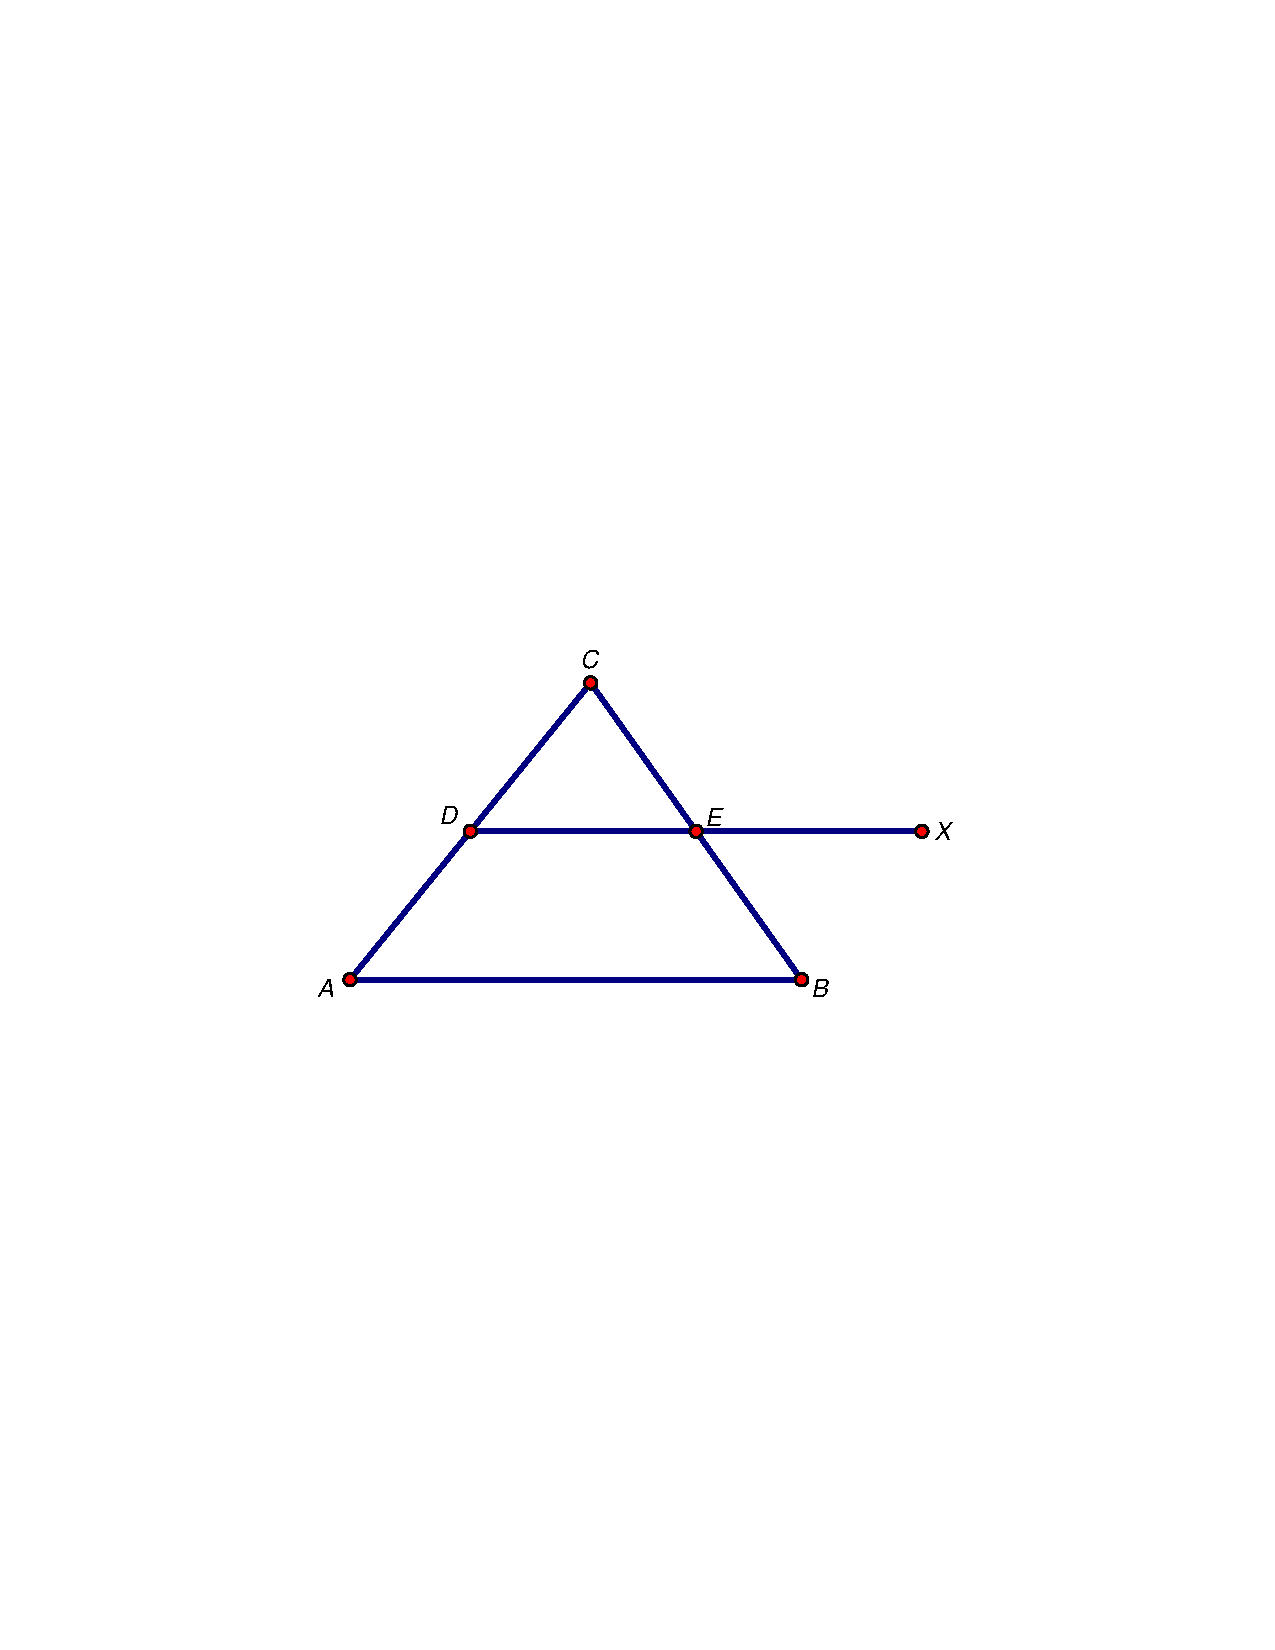
\includegraphics[scale=0.7]{midsegment1.pdf}
\end{image}
\end{problem}

\end{document}

%\input some version of the CMP dilation activity
%\documentclass[handout]{ximera}
\documentclass{ximera}

\usepackage{gensymb}
\usepackage{tabularx}
\usepackage{mdframed}
\usepackage{pdfpages}
%\usepackage{chngcntr}

\let\problem\relax
\let\endproblem\relax

\newcommand{\property}[2]{#1#2}




\newtheoremstyle{SlantTheorem}{\topsep}{\fill}%%% space between body and thm
 {\slshape}                      %%% Thm body font
 {}                              %%% Indent amount (empty = no indent)
 {\bfseries\sffamily}            %%% Thm head font
 {}                              %%% Punctuation after thm head
 {3ex}                           %%% Space after thm head
 {\thmname{#1}\thmnumber{ #2}\thmnote{ \bfseries(#3)}} %%% Thm head spec
\theoremstyle{SlantTheorem}
\newtheorem{problem}{Problem}[]

%\counterwithin*{problem}{section}



%%%%%%%%%%%%%%%%%%%%%%%%%%%%Jenny's code%%%%%%%%%%%%%%%%%%%%

%%% Solution environment
%\newenvironment{solution}{
%\ifhandout\setbox0\vbox\bgroup\else
%\begin{trivlist}\item[\hskip \labelsep\small\itshape\bfseries Solution\hspace{2ex}]
%\par\noindent\upshape\small
%\fi}
%{\ifhandout\egroup\else
%\end{trivlist}
%\fi}
%
%
%%% instructorIntro environment
%\ifhandout
%\newenvironment{instructorIntro}[1][false]%
%{%
%\def\givenatend{\boolean{#1}}\ifthenelse{\boolean{#1}}{\begin{trivlist}\item}{\setbox0\vbox\bgroup}{}
%}
%{%
%\ifthenelse{\givenatend}{\end{trivlist}}{\egroup}{}
%}
%\else
%\newenvironment{instructorIntro}[1][false]%
%{%
%  \ifthenelse{\boolean{#1}}{\begin{trivlist}\item[\hskip \labelsep\bfseries Instructor Notes:\hspace{2ex}]}
%{\begin{trivlist}\item[\hskip \labelsep\bfseries Instructor Notes:\hspace{2ex}]}
%{}
%}
%% %% line at the bottom} 
%{\end{trivlist}\par\addvspace{.5ex}\nobreak\noindent\hung} 
%\fi
%
%


\let\instructorNotes\relax
\let\endinstructorNotes\relax
%%% instructorNotes environment
\ifhandout
\newenvironment{instructorNotes}[1][false]%
{%
\def\givenatend{\boolean{#1}}\ifthenelse{\boolean{#1}}{\begin{trivlist}\item}{\setbox0\vbox\bgroup}{}
}
{%
\ifthenelse{\givenatend}{\end{trivlist}}{\egroup}{}
}
\else
\newenvironment{instructorNotes}[1][false]%
{%
  \ifthenelse{\boolean{#1}}{\begin{trivlist}\item[\hskip \labelsep\bfseries {\Large Instructor Notes: \\} \hspace{\textwidth} ]}
{\begin{trivlist}\item[\hskip \labelsep\bfseries {\Large Instructor Notes: \\} \hspace{\textwidth} ]}
{}
}
{\end{trivlist}}
\fi


%% Suggested Timing
\newcommand{\timing}[1]{{\bf Suggested Timing: \hspace{2ex}} #1}




\hypersetup{
    colorlinks=true,       % false: boxed links; true: colored links
    linkcolor=blue,          % color of internal links (change box color with linkbordercolor)
    citecolor=green,        % color of links to bibliography
    filecolor=magenta,      % color of file links
    urlcolor=cyan           % color of external links
}

\title{Similarities}
\author{Bart Snapp and Brad Findell}

\outcome{Learning outcome goes here.}

\begin{document}
\begin{abstract}
Abstract goes here.  
\end{abstract}
\maketitle

\begin{teachingnote}
Precede this with the Connected Math Program's stretching activity, which doesn't take a whole class.  
Supplies:  rubber bands, extra paper, tape.   
In the examples, include some pairs that are not similar.  Somehow require that they actually do the zooming.  Actually measure from eye to plastic bag and from eye paper to find the scale factor.  Use string for the measuring.  Use a sighting activity to the board.
\end{teachingnote}

\begin{problem}
Based on your experience with the stretching activity, write a definition of dilation.  Be sure to indicate (1) what it takes to specify the transformation, and (2) how to produce the image of a given point.  
\vspace{0.6in}
\end{problem}

\begin{problem}
Based on your experience with the stretching activity, describe for a dilation: 
\begin{enumerate}
\item What happens to line segments? 
\vspace{0.2in}
\item What happens to angles?  
\vspace{0.2in}
\item What happens to lines passing through the center of the dilation?
\vspace{0.2in}
\item What happens to lines not passing through the center of the dilation?
\vspace{0.2in}
\end{enumerate}
\end{problem}

%Every dilation has the following properties:
%\begin{enumerate}[(i)]
%\item It maps lines to lines, rays to rays, and segments to segments.
%\item It changes distance by a factor of $r$, where $r$ is the scale factor of the dilation.
%\item It maps every line passing through the center of dilation to itself, and it maps every line not passing through the center of the dilation to a parallel line.  
%\item It preserves angle measure.
%\end{enumerate}

\begin{definition}
A geometric figure is \emph{simliar} to another if the second can be obtained from the first by a sequence of rotations, reflections, translations, and dilations.  
\end{definition}

\begin{problem}
For each of the pairs of objects on the following pages, do the following:  
\begin{enumerate}
\item Trace the smaller figure on plastic.  Then close one eye and try to hold the plastic between your eye and the paper so that the tracing ``exactly'' covers the larger figure.   Be sure that the plane of the paper and the plane of the plastic are parallel.  (Why does this matter?) 
\item If the objects are similar, find a sequence of rotations, reflections, translations, and dilations that takes one figure onto the other.  
\item If the objects are similar, try to find a single dilation that demonstrates the similarity.   If you cannot find such a dilation, explain how you know you cannot.  
\end{enumerate}
\end{problem}
\vfill

\begin{image}
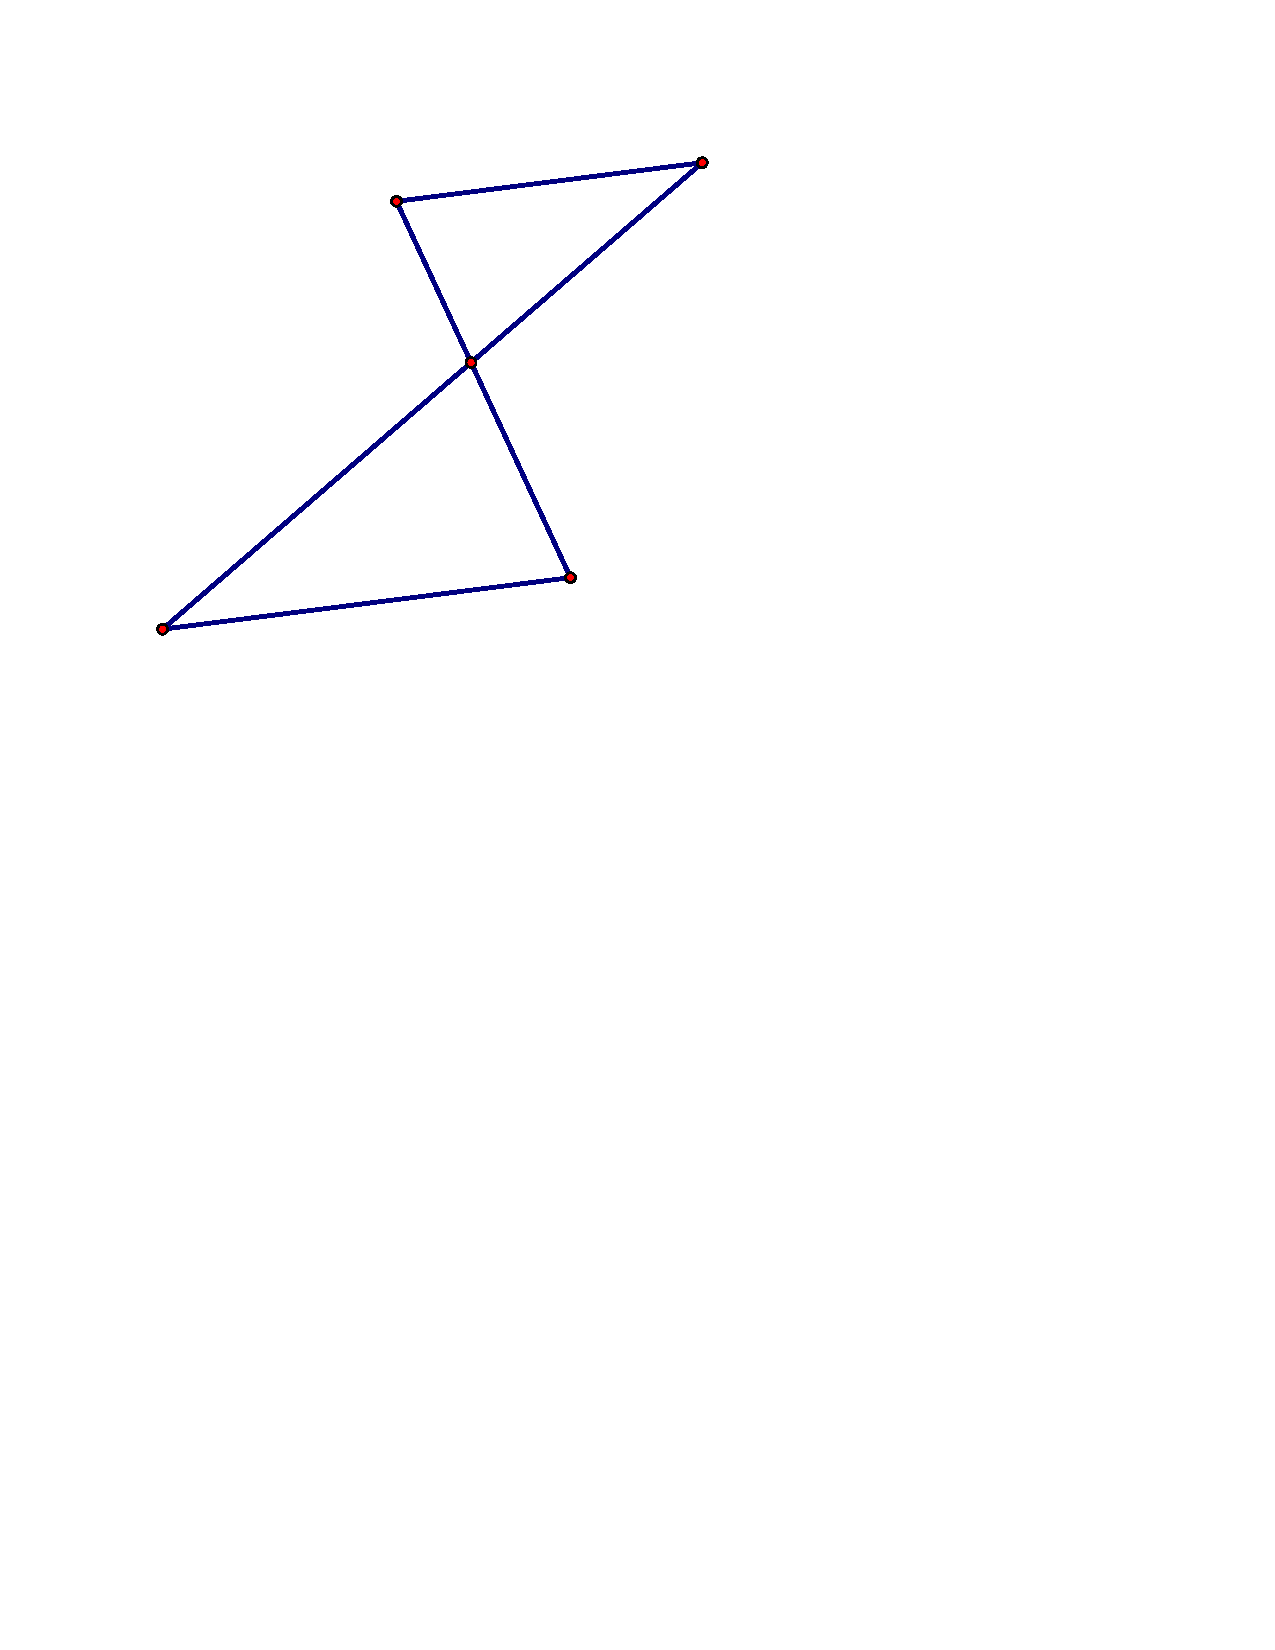
\includegraphics{similarTriangles1}
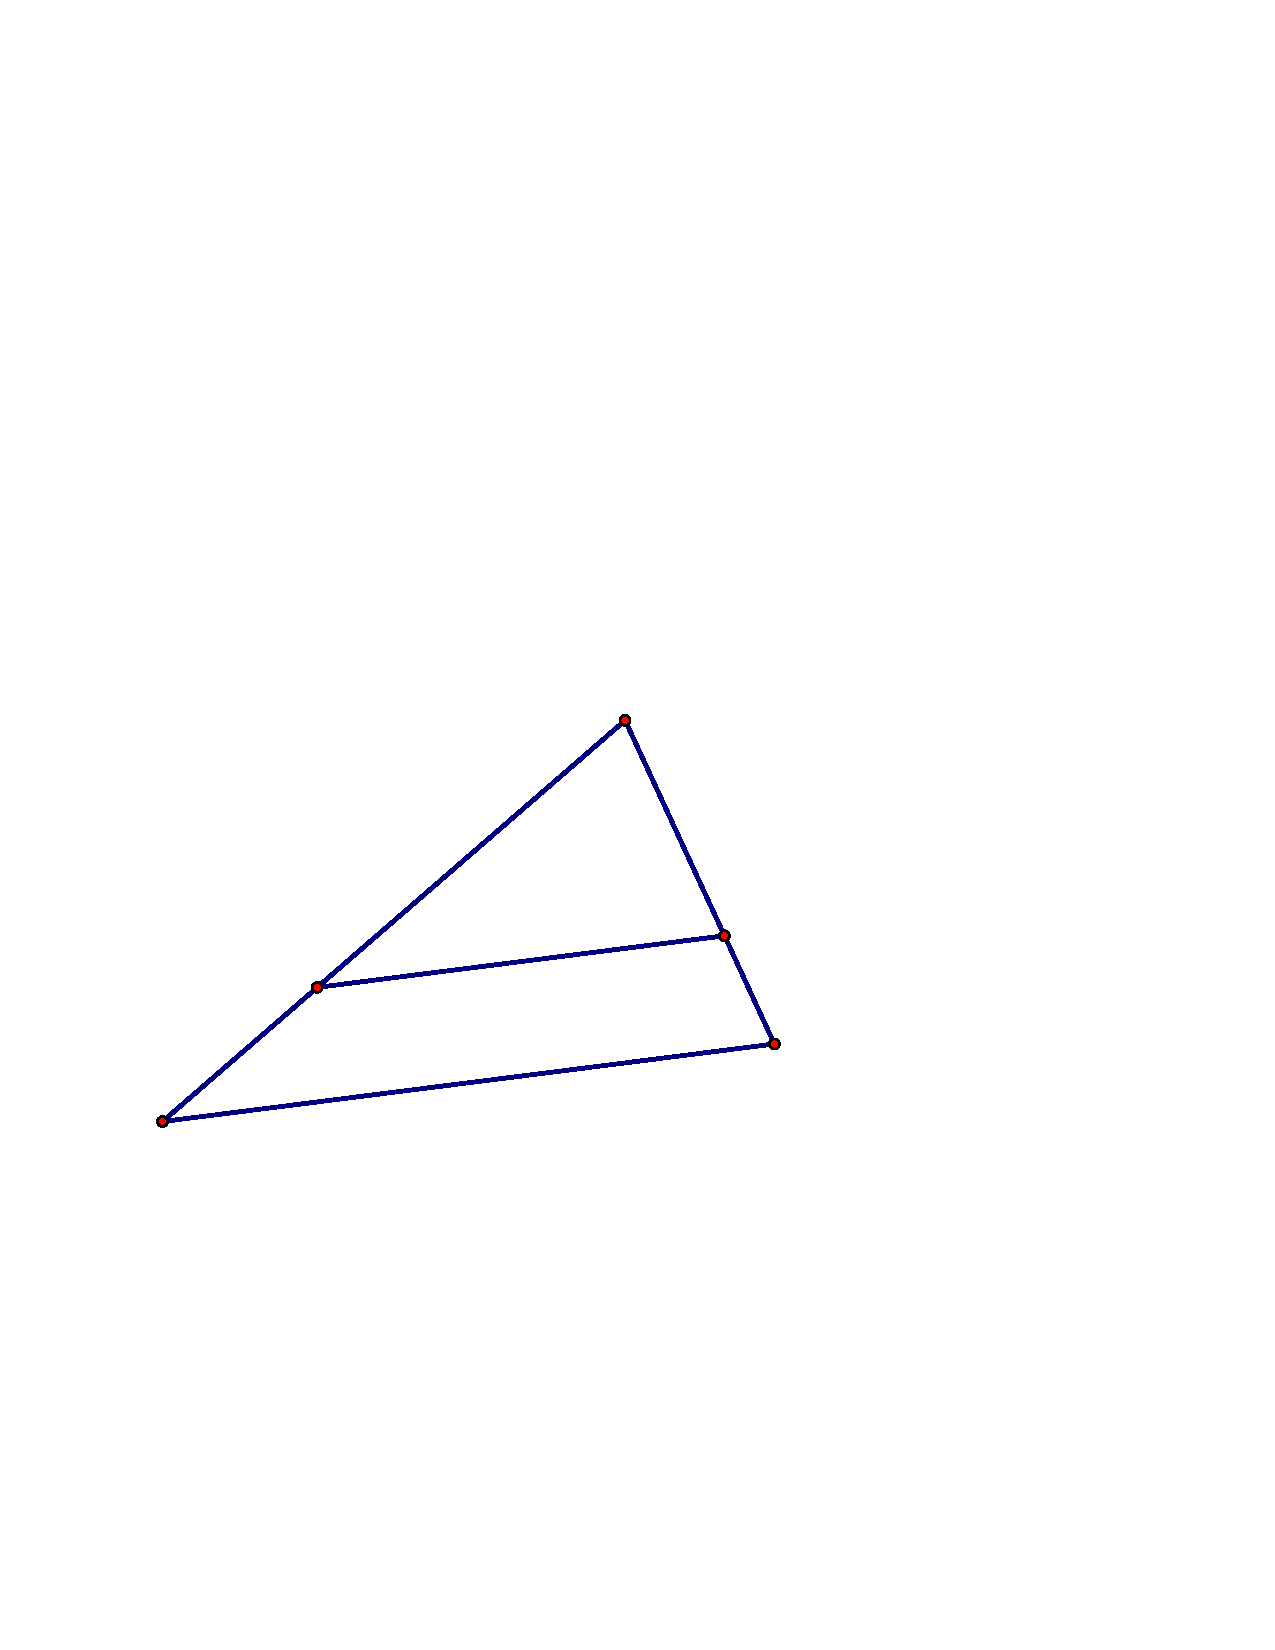
\includegraphics{similarTriangles2}
\end{image}

\vfill
\newpage
\vfill
\begin{image}
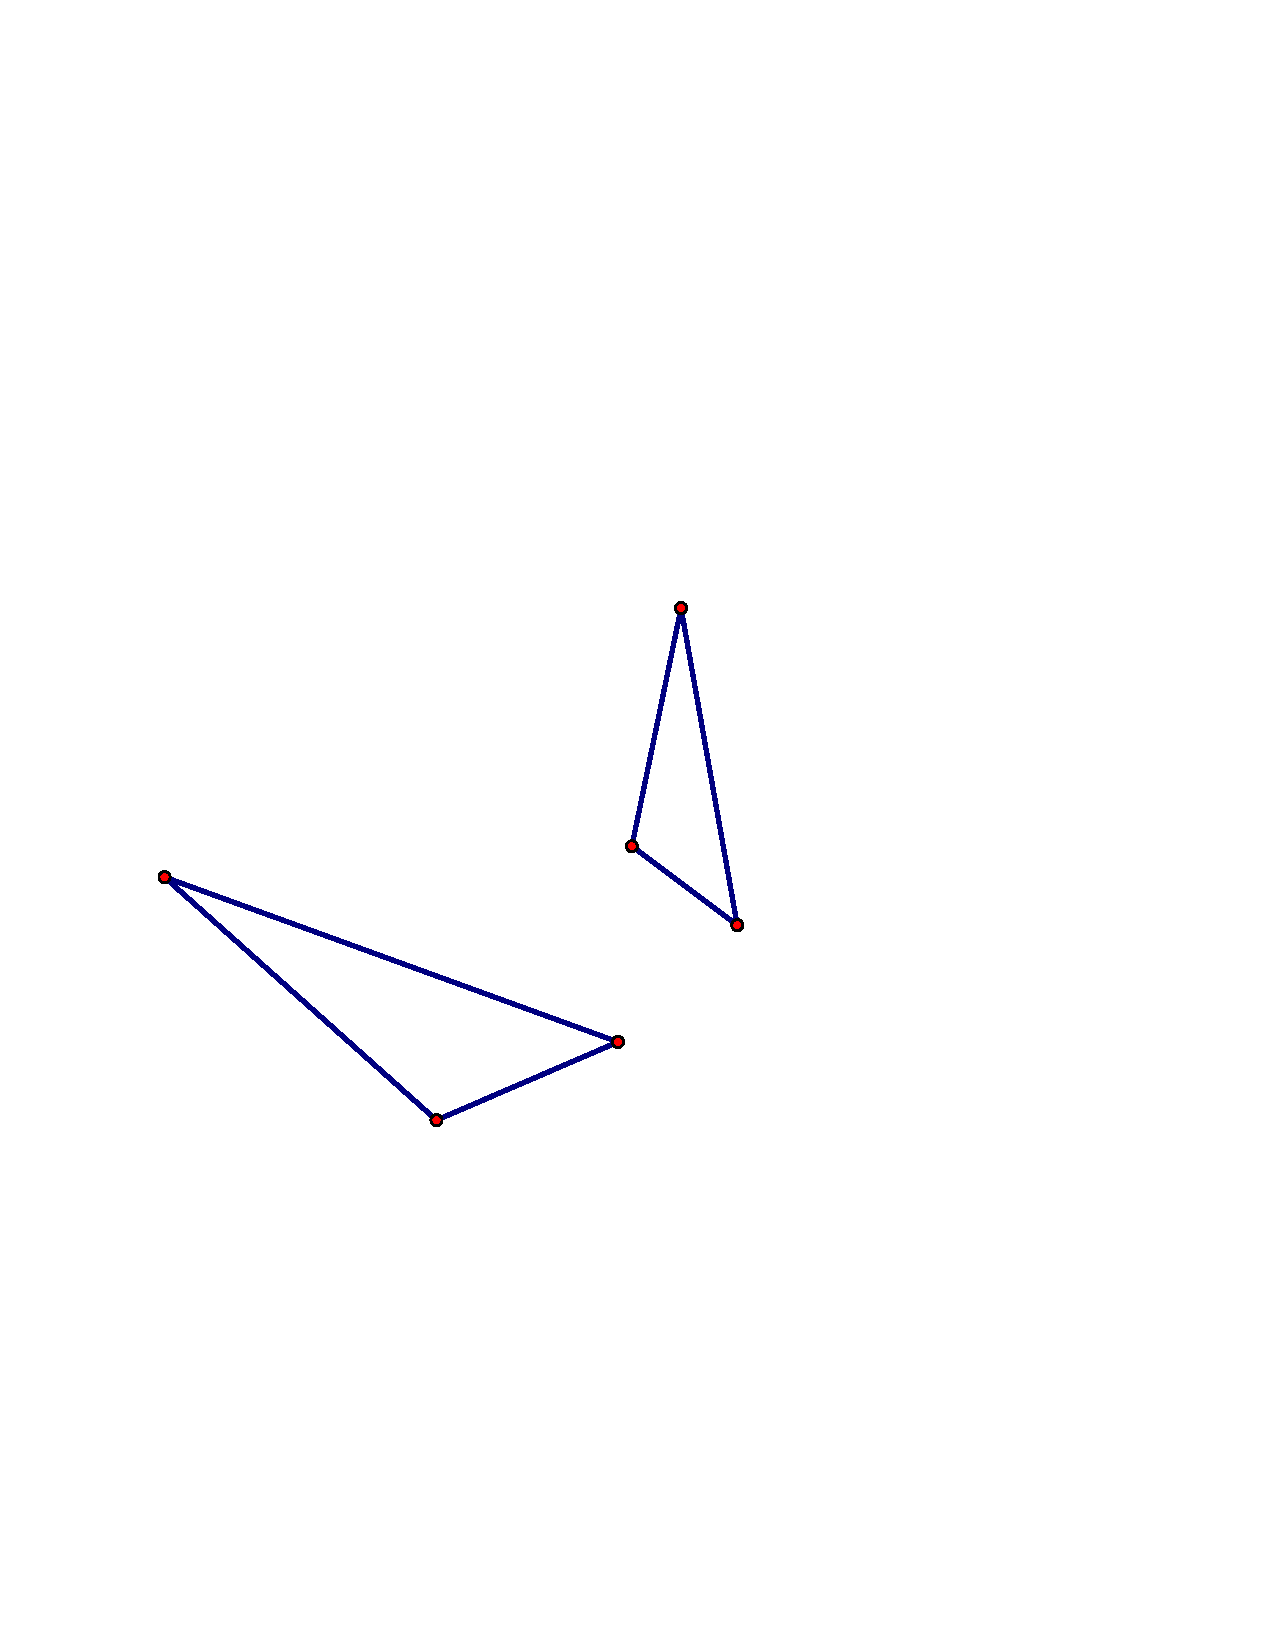
\includegraphics{similarTriangles3}
\includegraphics[scale=0.6]{similarTriangles5}
\end{image}
\vfill
\newpage
\begin{problem}
Describe a general (and foolproof) way of demonstrating that any two circles are 
similar.%\standardhs{G-C.1} 
\fixnote{Cite G-C.1}
\end{problem}
\vfill
\begin{image}
\includegraphics{similarCircles1}
\end{image}
\vfill
\newpage

\begin{problem}
Describe a general (and foolproof) way of demonstrating that any two parabolas are similar. 
\end{problem}
\vfill
\begin{image}
\includegraphics{similarParabolas1}
\includegraphics{similarParabolas2}
\end{image}
\vfill

\end{document}

%\documentclass[handout]{ximera}
\documentclass[nooutcomes]{ximera}

\usepackage{gensymb}
\usepackage{tabularx}
\usepackage{mdframed}
\usepackage{pdfpages}
%\usepackage{chngcntr}

\let\problem\relax
\let\endproblem\relax

\newcommand{\property}[2]{#1#2}




\newtheoremstyle{SlantTheorem}{\topsep}{\fill}%%% space between body and thm
 {\slshape}                      %%% Thm body font
 {}                              %%% Indent amount (empty = no indent)
 {\bfseries\sffamily}            %%% Thm head font
 {}                              %%% Punctuation after thm head
 {3ex}                           %%% Space after thm head
 {\thmname{#1}\thmnumber{ #2}\thmnote{ \bfseries(#3)}} %%% Thm head spec
\theoremstyle{SlantTheorem}
\newtheorem{problem}{Problem}[]

%\counterwithin*{problem}{section}



%%%%%%%%%%%%%%%%%%%%%%%%%%%%Jenny's code%%%%%%%%%%%%%%%%%%%%

%%% Solution environment
%\newenvironment{solution}{
%\ifhandout\setbox0\vbox\bgroup\else
%\begin{trivlist}\item[\hskip \labelsep\small\itshape\bfseries Solution\hspace{2ex}]
%\par\noindent\upshape\small
%\fi}
%{\ifhandout\egroup\else
%\end{trivlist}
%\fi}
%
%
%%% instructorIntro environment
%\ifhandout
%\newenvironment{instructorIntro}[1][false]%
%{%
%\def\givenatend{\boolean{#1}}\ifthenelse{\boolean{#1}}{\begin{trivlist}\item}{\setbox0\vbox\bgroup}{}
%}
%{%
%\ifthenelse{\givenatend}{\end{trivlist}}{\egroup}{}
%}
%\else
%\newenvironment{instructorIntro}[1][false]%
%{%
%  \ifthenelse{\boolean{#1}}{\begin{trivlist}\item[\hskip \labelsep\bfseries Instructor Notes:\hspace{2ex}]}
%{\begin{trivlist}\item[\hskip \labelsep\bfseries Instructor Notes:\hspace{2ex}]}
%{}
%}
%% %% line at the bottom} 
%{\end{trivlist}\par\addvspace{.5ex}\nobreak\noindent\hung} 
%\fi
%
%


\let\instructorNotes\relax
\let\endinstructorNotes\relax
%%% instructorNotes environment
\ifhandout
\newenvironment{instructorNotes}[1][false]%
{%
\def\givenatend{\boolean{#1}}\ifthenelse{\boolean{#1}}{\begin{trivlist}\item}{\setbox0\vbox\bgroup}{}
}
{%
\ifthenelse{\givenatend}{\end{trivlist}}{\egroup}{}
}
\else
\newenvironment{instructorNotes}[1][false]%
{%
  \ifthenelse{\boolean{#1}}{\begin{trivlist}\item[\hskip \labelsep\bfseries {\Large Instructor Notes: \\} \hspace{\textwidth} ]}
{\begin{trivlist}\item[\hskip \labelsep\bfseries {\Large Instructor Notes: \\} \hspace{\textwidth} ]}
{}
}
{\end{trivlist}}
\fi


%% Suggested Timing
\newcommand{\timing}[1]{{\bf Suggested Timing: \hspace{2ex}} #1}




\hypersetup{
    colorlinks=true,       % false: boxed links; true: colored links
    linkcolor=blue,          % color of internal links (change box color with linkbordercolor)
    citecolor=green,        % color of links to bibliography
    filecolor=magenta,      % color of file links
    urlcolor=cyan           % color of external links
}

\title{Side-Splitter Theorems}
\author{Bart Snapp and Brad Findell}

\outcome{Learning outcome goes here.}

\begin{document}
\begin{abstract}
  We prove fundamental theorems about similar triangles.
\end{abstract}
\maketitle

In this activity, we will show that the properties of dilations, which you noticed in a previous activity, can be proven \emph{without} using facts about transversals and parallel lines.  Instead, we use the area formula for triangles.  \emph{Note: For a given base, draw the corresponding altitude to reason about a triangle's area.}

\section*{Background: Areas of triangles}
\begin{question}
For the triangle area formula to be valid, what must be true about the base and height measurements?
\vfill
\end{question}
%\QM

\begin{problem}
Suppose the area of $\triangle SPR = 8$ square inches and the area of $\triangle QPR = 5$ square inches.  
\begin{enumerate}
\item Thinking of $SR$ and $RQ$ as bases of these triangles, respectively, what are their heights?  \item Then what can you say about $\frac{SR}{RQ}$?  What about $\frac{SR}{SQ}$?  
\item What can you say generally about how these ratios depend upon the areas of the triangles?  
\end{enumerate}
\begin{image}
\includegraphics[scale=0.65]{sideSplitter1}
\end{image}
\vfill
\end{problem}

\newpage
\begin{problem}
For the trapezoid below, explain why the area of $\triangle BAD$ is equal to the area of $\triangle BAC$.  Name two other triangles that have the same area.
\begin{image}
\includegraphics[scale=0.65]{sideSplitter2}
\end{image}
\vfill
\end{problem}

\begin{problem}
For the parallelogram below, which triangle has the greatest area: $\triangle XYZ$, $\triangle WXY$, $\triangle ZWX$, or $\triangle YZW$?  Explain.  
\begin{image}
\includegraphics[scale=0.65]{sideSplitter3}
\end{image}
\vfill
\end{problem}

\newpage
\section*{Side Splitting}
\begin{teachingnote}
An important objective in the next two problems is the habit of using an equation string, one modification at a time, to show that two expressions are equivalent.
\end{teachingnote}

\begin{problem}
Prove the \textbf{Parallel-Side Theorem}:  If a line in a triangle is parallel to a side of a triangle, then it splits the other sides of the triangle proportionally. 
\begin{image}
\includegraphics[scale=0.8]{sideSplitter4}
\end{image}
\begin{enumerate}
\item How do the areas of $\triangle ADE$ and $\triangle DBE$ relate to $AD$ and $DB$?  Explain.  
\item How do the areas of $\triangle ADE$ and $\triangle ECD$ relate to $AE$ and $EC$?  Explain. 
\item How do the areas of $\triangle DBE$ and $\triangle ECD$ compare?  Explain.  
\item Use the previous results to show that $\frac{DB}{AD} = \frac{EC}{AE}$.  
\item What the heck did we just do?  What does this say?
\item Where in the proof did we use the fact that $\overline{DE} \parallel \overline{BC}$?  
\end{enumerate}
\vfill
\end{problem}

\newpage
\begin{teachingnote}
In the following argument, the triangles refer to their areas.  
Two pairs of triangles with the same height and different bases:  
\[
\frac{DB}{AD} = \frac{\triangle DBE}{\triangle ADE}
\]
\[
\frac{EC}{AE} = \frac{\triangle ECD}{\triangle ADE}
\]
Because of the parallel lines, a pair of triangles with the same height and the same base:  
\[
\triangle DBE = \triangle ECD
\]
Putting this together, we have:  
\[
\frac{DB}{AD} = \frac{\triangle DBE}{\triangle ADE} = \frac{\triangle ECD}{\triangle ADE}
=\frac{EC}{AE}
\]
\end{teachingnote}


\begin{problem}
Use some algebra to show, in the previous picture, that $\frac{AB}{AD} = \frac{AC}{AE}$.
\vspace{1in}
\end{problem}

\begin{teachingnote}
\[
\frac{AB}{AD} = \frac{AD+DB}{AD} = 1 + \frac{DB}{AD} =  1 + \frac{EC}{AE} 
= \frac{AE + EC}{AE} = \frac{AC}{AE}
\]
\end{teachingnote}

\begin{problem}
Prove:  Next we prove, in the previous figure, that $ \frac{BC}{DE} = \frac{AB}{AD} = \frac{AC}{AE}$.  Here are the steps.  
\begin{enumerate}
\item How do we know that $\angle ADE \cong \angle ABC$?  
\item Translate $\triangle ADE$ by the vector $\overrightarrow{DB}$ so that the image $\angle A'D'E'$ of $\angle ADE$ coincides with $\angle ABC$.  Draw a picture of the result.  
\item What segments are parallel now?  How do you know?  
\item Now explain why $\frac{BC}{DE} = \frac{AB}{AD} = \frac{AC}{AE}$ is equal to a common ratio from the previous problem.  
\end{enumerate}
\vfill
\end{problem}

\newpage

\begin{problem}
Explain briefly how the Parallel-Side Theorem implies the AA criterion for triangle similarity.  (Hint: Be sure to use the definition of similarity in terms of basic rigid motions and dilations.)  
% Hint:  You need to begin with two triangles that have two pairs of congrent angles.  You need to show (generally) that there exists a sequence of basic rigid motions and dilations that maps one triangle onto the other.  Be sure to consider how you would know whether a reflection is needed as one of the basic rigid motions.  
\vfill
\end{problem}

\begin{problem}
The \textbf{Split-Side Theorem} is the converse of the Parallel-Side Theorem.   
\begin{enumerate}
\item State the Split-Side Theorem.   
% If a line in a triangle splits two sides proportionally, then it is parallel to the third side of the triangle.
\item Prove the Split-Side Theorem.  (Hint:  Using the previous figures, draw a line through $D$ and parallel to $\overline{BC}$, and let $X$ be the point where the new line intersects $\overline{AC}$.  By the previous results, $\overline{DX}$ divides the sides proportionally.  Then argue that $E$ and $X$ must be the same point.)  
\end{enumerate}
\vfill
\end{problem}

\newpage

\begin{problem}
Use the Split-Side Theorem to justify the following properties of a dilation given by a center and a scale factor:
\begin{enumerate}
\item A dilation takes a line not passing through the center of the dilation to a parallel line, and leaves a line passing through the center unchanged.
\item The dilation of a line segment is longer or shorter in the ratio given by the scale factor.
\end{enumerate}
% Hint: You need to begin with a dilation, and you need to show that it has the listed properties.  In addition to the Split-Side Theorem, you may also use other results established in this activity. 
\vfill
\end{problem}

\begin{problem}
Explain briefly how the Split-Side Theorem establishes the SAS criterion for triangle similarity.  
\vfill
\end{problem}


\end{document}

%\documentclass[handout]{ximera}
\documentclass[nooutcomes]{ximera}

\usepackage{gensymb}
\usepackage{tabularx}
\usepackage{mdframed}
\usepackage{pdfpages}
%\usepackage{chngcntr}

\let\problem\relax
\let\endproblem\relax

\newcommand{\property}[2]{#1#2}




\newtheoremstyle{SlantTheorem}{\topsep}{\fill}%%% space between body and thm
 {\slshape}                      %%% Thm body font
 {}                              %%% Indent amount (empty = no indent)
 {\bfseries\sffamily}            %%% Thm head font
 {}                              %%% Punctuation after thm head
 {3ex}                           %%% Space after thm head
 {\thmname{#1}\thmnumber{ #2}\thmnote{ \bfseries(#3)}} %%% Thm head spec
\theoremstyle{SlantTheorem}
\newtheorem{problem}{Problem}[]

%\counterwithin*{problem}{section}



%%%%%%%%%%%%%%%%%%%%%%%%%%%%Jenny's code%%%%%%%%%%%%%%%%%%%%

%%% Solution environment
%\newenvironment{solution}{
%\ifhandout\setbox0\vbox\bgroup\else
%\begin{trivlist}\item[\hskip \labelsep\small\itshape\bfseries Solution\hspace{2ex}]
%\par\noindent\upshape\small
%\fi}
%{\ifhandout\egroup\else
%\end{trivlist}
%\fi}
%
%
%%% instructorIntro environment
%\ifhandout
%\newenvironment{instructorIntro}[1][false]%
%{%
%\def\givenatend{\boolean{#1}}\ifthenelse{\boolean{#1}}{\begin{trivlist}\item}{\setbox0\vbox\bgroup}{}
%}
%{%
%\ifthenelse{\givenatend}{\end{trivlist}}{\egroup}{}
%}
%\else
%\newenvironment{instructorIntro}[1][false]%
%{%
%  \ifthenelse{\boolean{#1}}{\begin{trivlist}\item[\hskip \labelsep\bfseries Instructor Notes:\hspace{2ex}]}
%{\begin{trivlist}\item[\hskip \labelsep\bfseries Instructor Notes:\hspace{2ex}]}
%{}
%}
%% %% line at the bottom} 
%{\end{trivlist}\par\addvspace{.5ex}\nobreak\noindent\hung} 
%\fi
%
%


\let\instructorNotes\relax
\let\endinstructorNotes\relax
%%% instructorNotes environment
\ifhandout
\newenvironment{instructorNotes}[1][false]%
{%
\def\givenatend{\boolean{#1}}\ifthenelse{\boolean{#1}}{\begin{trivlist}\item}{\setbox0\vbox\bgroup}{}
}
{%
\ifthenelse{\givenatend}{\end{trivlist}}{\egroup}{}
}
\else
\newenvironment{instructorNotes}[1][false]%
{%
  \ifthenelse{\boolean{#1}}{\begin{trivlist}\item[\hskip \labelsep\bfseries {\Large Instructor Notes: \\} \hspace{\textwidth} ]}
{\begin{trivlist}\item[\hskip \labelsep\bfseries {\Large Instructor Notes: \\} \hspace{\textwidth} ]}
{}
}
{\end{trivlist}}
\fi


%% Suggested Timing
\newcommand{\timing}[1]{{\bf Suggested Timing: \hspace{2ex}} #1}




\hypersetup{
    colorlinks=true,       % false: boxed links; true: colored links
    linkcolor=blue,          % color of internal links (change box color with linkbordercolor)
    citecolor=green,        % color of links to bibliography
    filecolor=magenta,      % color of file links
    urlcolor=cyan           % color of external links
}

\title{Trigonometry Checkup}
\author{Bart Snapp and Brad Findell}

\outcome{Learning outcome goes here.}

\begin{document}
\begin{abstract}
  We review trigonometry.
\end{abstract}
\maketitle

\begin{teachingnote}
This activity can be done either as part of similarity or as a preactivity for Circular Trigonometry.  Perhaps recommend a special office hour for this.  
\end{teachingnote}
This activity is intended to remind you of key ideas from high school trigonometry. 

\begin{problem}
What are the ratios of side lengths in a $45^\circ$-$45^\circ$-$90^\circ$ triangle?  Explain where the ratios come from, including why they work for any such triangle, no matter what size.  (Hint: Use the Pythagorean Theorem.)
\end{problem}

\vspace{0.1in}

\begin{problem}
What are the ratios of side lengths in a $30^\circ$-$60^\circ$-$90^\circ$ triangle?  Explain where those the come from.  (Hint: How might an equilateral triangle help.)
\end{problem}

\vspace{0.1in}

\begin{problem}
Consider the right triangle below with an angle of $\alpha$, sides of length $x$ and $y$, and hypotenuse of length $r$, as labeled.  
%$$\includegraphics[scale=0.8]{../graphics/rightTriangle}$$
\[
\definecolor{qqwuqq}{rgb}{0.,0.392,0.}
\definecolor{qqqqff}{rgb}{0.,0.,1.}
\begin{tikzpicture}[line cap=round,line join=round,>=triangle 45,x=1.0cm,y=1.0cm]
\clip(-0.36,-0.34) rectangle (4.1,2.2);
\draw [shift={(0.,0.)},line width=0.8pt,color=qqwuqq,fill=qqwuqq,fill opacity=0.1] (0,0) -- (0.:0.5) arc (0.:29.745:0.5) -- cycle;
\draw [shift={(3.5,2.)},line width=0.8pt,color=qqwuqq,fill=qqwuqq,fill opacity=0.1] (0,0) -- (-150.26:0.5) arc (-150.26:-90.:0.5) -- cycle;
\draw[line width=0.8pt,color=qqwuqq,fill=qqwuqq,fill opacity=0.1] (3.5,0.28) -- (3.22,0.28) -- (3.22,0.) -- (3.5,0.) -- cycle; 
\draw [line width=0.8pt] (0.,0.)-- (3.5,2.);
\draw [line width=0.8pt] (3.5,2.)-- (3.5,0.);
\draw [line width=0.8pt] (3.5,0.)-- (0.,0.);
%\draw [fill=qqqqff] (0.,0.) circle (1.2pt);
%\draw [fill=qqqqff] (3.5,0.) circle (1.2pt);
%\draw [fill=qqqqff] (3.5,2.) circle (1.2pt);
\draw[color=qqwuqq] (0.85,0.2) node {$\alpha$};
%\draw[color=qqwuqq] (3.2,1.33) node {$\beta$};
\draw (1.8,-.2) node {$x$};
\draw (1.8,1.23) node {$r$};
\draw (3.7,1.) node {$y$};
\end{tikzpicture}
\]
\begin{enumerate}
\item If we imagine angle $\alpha$ is fixed, why are ratios of pairs of side lengths the same, no matter the size of the triangle?\margincomment{CCSS G-SRT.6. Understand that by similarity, side ratios in right triangles
  are properties of the angles in the triangle, leading to definitions
  of trigonometric ratios for acute angles.}
\vspace{0.3in}
\item Using the triangle above (and your memory of Precalculus), write down the side-length ratios for sine, cosine, and tangent:  
$$\sin\alpha = \hspace{1in} \cos\alpha = \hspace{1in} \tan\alpha =$$
\vspace{0.1in}
\item What values of $\alpha$ make sense in \emph{right triangle trigonometry}?  (We overcome these bounds later in circular trigonometry.)  
\vspace{0.3in}
\item What does it mean to say that these ratios depend upon the angle $\alpha$?  
\vspace{0.3in}
\item Why is only one of the triangle's three angles necessary in defining these ratios?  
\vspace{0.3in}
\end{enumerate}
\end{problem}

\begin{problem}
Use your work so far to find the following trigonometric ratios:
\begin{enumerate}
\itemsep 12pt
\item $\sin 30^\circ = \hspace{1in} \cos30^\circ = \hspace{1in} \tan30^\circ =$
\item $\sin 45^\circ = \hspace{1in} \cos45^\circ = \hspace{1in} \tan45^\circ =$
\item $\sin 60^\circ = \hspace{1in} \cos60^\circ = \hspace{1in} \tan60^\circ =$
\item $\sin 0^\circ = \hspace{1.08in} \cos0^\circ = \hspace{1.08in} \tan0^\circ =$
\end{enumerate}
\end{problem}

\vspace{0.2in}

\begin{problem}
You may recall the identity $\sin^2\theta+\cos^2\theta=1$.\margincomment{CCSS F-TF.8.  Prove the Pythagorean identity $\sin^2(\theta) + \cos^2(\theta) = 1$ and use it
  to find $\sin(\theta)$, $\cos(\theta)$, or $\tan(\theta)$ given $\sin(\theta)$, $\cos(\theta)$, or $\tan(\theta)$
  and the quadrant of the angle.}
\begin{enumerate}
\item Explain why the equation is true.  
\vspace{0.3in}
\item Why is it called an identity? 
\vspace{0.3in}
\item Why is it called a Pythagorean identity?  
\vspace{0.3in}
\end{enumerate}
\end{problem}

\begin{problem}
In right triangle trigonometry, there are indeed two acute angles, as shown in the figure below.\margincomment{CCSS G-SRT.7. Explain and use the relationship between the sine and cosine of
  complementary angles.}
%$$\includegraphics[scale=0.8]{../graphics/rightTriangle2}$$
\[
\definecolor{qqwuqq}{rgb}{0.,0.392,0.}
\definecolor{qqqqff}{rgb}{0.,0.,1.}
\begin{tikzpicture}[line cap=round,line join=round,>=triangle 45,x=1.0cm,y=1.0cm]
\clip(-0.36,-0.36) rectangle (4.1,2.2);
\draw [shift={(0.,0.)},line width=0.8pt,color=qqwuqq,fill=qqwuqq,fill opacity=0.1] (0,0) -- (0.:0.5) arc (0.:29.745:0.5) -- cycle;
\draw [shift={(3.5,2.)},line width=0.8pt,color=qqwuqq,fill=qqwuqq,fill opacity=0.1] (0,0) -- (-150.26:0.5) arc (-150.26:-90.:0.5) -- cycle;
\draw[line width=0.8pt,color=qqwuqq,fill=qqwuqq,fill opacity=0.1] (3.5,0.28) -- (3.22,0.28) -- (3.22,0.) -- (3.5,0.) -- cycle; 
\draw [line width=0.8pt] (0.,0.)-- (3.5,2.);
\draw [line width=0.8pt] (3.5,2.)-- (3.5,0.);
\draw [line width=0.8pt] (3.5,0.)-- (0.,0.);
%\draw [fill=qqqqff] (0.,0.) circle (1.2pt);
%\draw [fill=qqqqff] (3.5,0.) circle (1.2pt);
%\draw [fill=qqqqff] (3.5,2.) circle (1.2pt);
\draw[color=qqwuqq] (0.85,0.2) node {$\alpha$};
\draw[color=qqwuqq] (3.2,1.33) node {$\beta$};
\draw (1.8,-.2) node {$x$};
\draw (1.8,1.23) node {$r$};
\draw (3.7,1.) node {$y$};
\end{tikzpicture}
\]
\begin{enumerate}
\item How are the angles $\alpha$ and $\beta$ related?  Explain why.
\vspace{0.3in}
\item Using lengths in the above triangle, find the following ratios:    
$$\sin\alpha = \qquad\qquad\qquad \cos\alpha = $$
$$\sin\beta = \qquad\qquad\qquad \cos\beta = $$
\item What do you notice about the sine and cosine of complementary angles?  
\vspace{0.3in}
\item Explain why the result makes sense.  
\vspace{0.3in}
\end{enumerate}
\end{problem}

Given an angle and a side length of a right triangle, 
you can find the missing side lengths.\margincomment{CCSS G-SRT.8. Use trigonometric ratios and the Pythagorean Theorem to solve
  right triangles in applied problems.}
This is called ``solving the right triangle.''    And given the sine, cosine, or tangent of an angle, you can find the other two ratios.  (Hint: In either case, draw a triangle.)

%\begin{problem}
%A straight wire to the top of a flagpole meets the ground at a $25^\circ$ angle 30 feet from the base of the flag pole (on a flat lawn).  How high is the flagpole?  How long is the wire?  
%\end{problem}
%
%\vspace{0.5in}

\begin{problem}
Suppose $\sin\alpha = \frac{3}{5}$.  Then $\cos\alpha = \hspace{0.6in}$, $\tan\alpha = \hspace{0.6in}$.  
\end{problem}

\end{document}

%\documentclass[handout]{ximera}
\documentclass[nooutcomes]{ximera}

\usepackage{gensymb}
\usepackage{tabularx}
\usepackage{mdframed}
\usepackage{pdfpages}
%\usepackage{chngcntr}

\let\problem\relax
\let\endproblem\relax

\newcommand{\property}[2]{#1#2}




\newtheoremstyle{SlantTheorem}{\topsep}{\fill}%%% space between body and thm
 {\slshape}                      %%% Thm body font
 {}                              %%% Indent amount (empty = no indent)
 {\bfseries\sffamily}            %%% Thm head font
 {}                              %%% Punctuation after thm head
 {3ex}                           %%% Space after thm head
 {\thmname{#1}\thmnumber{ #2}\thmnote{ \bfseries(#3)}} %%% Thm head spec
\theoremstyle{SlantTheorem}
\newtheorem{problem}{Problem}[]

%\counterwithin*{problem}{section}



%%%%%%%%%%%%%%%%%%%%%%%%%%%%Jenny's code%%%%%%%%%%%%%%%%%%%%

%%% Solution environment
%\newenvironment{solution}{
%\ifhandout\setbox0\vbox\bgroup\else
%\begin{trivlist}\item[\hskip \labelsep\small\itshape\bfseries Solution\hspace{2ex}]
%\par\noindent\upshape\small
%\fi}
%{\ifhandout\egroup\else
%\end{trivlist}
%\fi}
%
%
%%% instructorIntro environment
%\ifhandout
%\newenvironment{instructorIntro}[1][false]%
%{%
%\def\givenatend{\boolean{#1}}\ifthenelse{\boolean{#1}}{\begin{trivlist}\item}{\setbox0\vbox\bgroup}{}
%}
%{%
%\ifthenelse{\givenatend}{\end{trivlist}}{\egroup}{}
%}
%\else
%\newenvironment{instructorIntro}[1][false]%
%{%
%  \ifthenelse{\boolean{#1}}{\begin{trivlist}\item[\hskip \labelsep\bfseries Instructor Notes:\hspace{2ex}]}
%{\begin{trivlist}\item[\hskip \labelsep\bfseries Instructor Notes:\hspace{2ex}]}
%{}
%}
%% %% line at the bottom} 
%{\end{trivlist}\par\addvspace{.5ex}\nobreak\noindent\hung} 
%\fi
%
%


\let\instructorNotes\relax
\let\endinstructorNotes\relax
%%% instructorNotes environment
\ifhandout
\newenvironment{instructorNotes}[1][false]%
{%
\def\givenatend{\boolean{#1}}\ifthenelse{\boolean{#1}}{\begin{trivlist}\item}{\setbox0\vbox\bgroup}{}
}
{%
\ifthenelse{\givenatend}{\end{trivlist}}{\egroup}{}
}
\else
\newenvironment{instructorNotes}[1][false]%
{%
  \ifthenelse{\boolean{#1}}{\begin{trivlist}\item[\hskip \labelsep\bfseries {\Large Instructor Notes: \\} \hspace{\textwidth} ]}
{\begin{trivlist}\item[\hskip \labelsep\bfseries {\Large Instructor Notes: \\} \hspace{\textwidth} ]}
{}
}
{\end{trivlist}}
\fi


%% Suggested Timing
\newcommand{\timing}[1]{{\bf Suggested Timing: \hspace{2ex}} #1}




\hypersetup{
    colorlinks=true,       % false: boxed links; true: colored links
    linkcolor=blue,          % color of internal links (change box color with linkbordercolor)
    citecolor=green,        % color of links to bibliography
    filecolor=magenta,      % color of file links
    urlcolor=cyan           % color of external links
}

\title{Please be Rational}
\author{Bart Snapp and Brad Findell}

\outcome{Learning outcome goes here.}

\begin{document}
\begin{abstract}
  We prove that the square root of two is not rational.
\end{abstract}
\maketitle

Let's see if we can give yet another proof that the square root of two
is not rational. Consider the following isosceles right triangle:
\begin{image}
\includegraphics{isorighttri.pdf}
\end{image}
\begin{problem}
Using the most famous theorem of all, how long is the unmarked side?
\end{problem}

\begin{problem} 
Suppose that the unmarked side has a rational length. In that case how
could we express it?
\end{problem}

\begin{problem}
Explain why there would then be a \textit{smallest} isosceles right
triangle with integer sides. Considering the problem above, how long
would the sides be? Draw and label a picture.
\end{problem}

\newpage
\begin{problem}
Now fold your smallest isosceles right triangle with integer sides
along the dotted line like so:
\begin{image}
\includegraphics{foldisorighttri.pdf}
\end{image}
Describe how to accomplish the fold, and explain why the figure is as marked.  
\end{problem}
\vspace{1in}

\begin{problem}
Explain how we have now found an isosceles right triangle with integer
sides that is now smaller than the smallest isosceles right triangle
with integer sides. Is this possible? What must we now conclude?
\end{problem}

\end{document}

%\documentclass[handout]{ximera}
\documentclass{ximera}

\usepackage{gensymb}
\usepackage{tabularx}
\usepackage{mdframed}
\usepackage{pdfpages}
%\usepackage{chngcntr}

\let\problem\relax
\let\endproblem\relax

\newcommand{\property}[2]{#1#2}




\newtheoremstyle{SlantTheorem}{\topsep}{\fill}%%% space between body and thm
 {\slshape}                      %%% Thm body font
 {}                              %%% Indent amount (empty = no indent)
 {\bfseries\sffamily}            %%% Thm head font
 {}                              %%% Punctuation after thm head
 {3ex}                           %%% Space after thm head
 {\thmname{#1}\thmnumber{ #2}\thmnote{ \bfseries(#3)}} %%% Thm head spec
\theoremstyle{SlantTheorem}
\newtheorem{problem}{Problem}[]

%\counterwithin*{problem}{section}



%%%%%%%%%%%%%%%%%%%%%%%%%%%%Jenny's code%%%%%%%%%%%%%%%%%%%%

%%% Solution environment
%\newenvironment{solution}{
%\ifhandout\setbox0\vbox\bgroup\else
%\begin{trivlist}\item[\hskip \labelsep\small\itshape\bfseries Solution\hspace{2ex}]
%\par\noindent\upshape\small
%\fi}
%{\ifhandout\egroup\else
%\end{trivlist}
%\fi}
%
%
%%% instructorIntro environment
%\ifhandout
%\newenvironment{instructorIntro}[1][false]%
%{%
%\def\givenatend{\boolean{#1}}\ifthenelse{\boolean{#1}}{\begin{trivlist}\item}{\setbox0\vbox\bgroup}{}
%}
%{%
%\ifthenelse{\givenatend}{\end{trivlist}}{\egroup}{}
%}
%\else
%\newenvironment{instructorIntro}[1][false]%
%{%
%  \ifthenelse{\boolean{#1}}{\begin{trivlist}\item[\hskip \labelsep\bfseries Instructor Notes:\hspace{2ex}]}
%{\begin{trivlist}\item[\hskip \labelsep\bfseries Instructor Notes:\hspace{2ex}]}
%{}
%}
%% %% line at the bottom} 
%{\end{trivlist}\par\addvspace{.5ex}\nobreak\noindent\hung} 
%\fi
%
%


\let\instructorNotes\relax
\let\endinstructorNotes\relax
%%% instructorNotes environment
\ifhandout
\newenvironment{instructorNotes}[1][false]%
{%
\def\givenatend{\boolean{#1}}\ifthenelse{\boolean{#1}}{\begin{trivlist}\item}{\setbox0\vbox\bgroup}{}
}
{%
\ifthenelse{\givenatend}{\end{trivlist}}{\egroup}{}
}
\else
\newenvironment{instructorNotes}[1][false]%
{%
  \ifthenelse{\boolean{#1}}{\begin{trivlist}\item[\hskip \labelsep\bfseries {\Large Instructor Notes: \\} \hspace{\textwidth} ]}
{\begin{trivlist}\item[\hskip \labelsep\bfseries {\Large Instructor Notes: \\} \hspace{\textwidth} ]}
{}
}
{\end{trivlist}}
\fi


%% Suggested Timing
\newcommand{\timing}[1]{{\bf Suggested Timing: \hspace{2ex}} #1}




\hypersetup{
    colorlinks=true,       % false: boxed links; true: colored links
    linkcolor=blue,          % color of internal links (change box color with linkbordercolor)
    citecolor=green,        % color of links to bibliography
    filecolor=magenta,      % color of file links
    urlcolor=cyan           % color of external links
}

\title{Rep-Tiles}
\author{Bart Snapp and Brad Findell}

\outcome{Learning outcome goes here.}

\begin{document}
\begin{abstract}
Abstract goes here.  
\end{abstract}
\maketitle

\begin{teachingnote}
Problems 1--3 can be a preactivity.  

Supplies: scissors, printed versions of the figures (so that students can cut them out), and a printed version of the summary table.   Students will need some time working with the figures, computing their areas and perimeters, and practicing arithmetic of radicals.   

An overall goal (across these activities and related homework) is that students use dimension to think about scaling. This needs development and discussion.  
\end{teachingnote}

A \textbf{rep-tile}\index{rep-tile} is a polygon where several copies of
a given rep-tile fit together to make a larger, similar, version of
itself. If $2$ copies are used, we call it a \textit{rep-2-tile}, if
$3$ copies are used, we call it a \textit{rep-3-tile}, and if $n$ copies
are used, we call it a \textit{rep-n-tile}.  Below is an example of a rectangle 
that is a rep-4-tile.
\begin{image}
\includegraphics[scale=0.6]{reptile1.pdf}
\end{image}
\begin{problem}
Explain why every parallelogram is a rep-4-tile. Give an example, and compare the perimeter and area of the larger figure to that of the original.
\end{problem}

\begin{problem}
Explain why every triangle is a rep-4-tile. Give an example, and compare the perimeter and area of the larger figure to that of the
original.
\end{problem}

\begin{problem}
Explain why every parallelogram and every triangle is a rep-9-tile. Give an example of each, and compare the perimeter and area of the larger triangle to that of the original. Can you generalize your result?  In other words, for what values of $n$ can you say that every parallelogram and every triangle is a rep-$n$-tile?  
\end{problem}

\begin{problem}
With a separate sheet of paper, draw and cut out:
\begin{enumerate}
\item An isosceles right triangle whose sides have lengths $1''$, $1''$, and $\sqrt{2}''$.
\item A rectangle whose sides have lengths $1''$ and $\sqrt{2}''$.
\end{enumerate}
Working with a partner, show that each of these polygons is a rep-2-tile.  And in each case,
how do the perimeter and area of the larger polygon compare to the perimeter and area of the original?
\end{problem}

\begin{problem}
With a fresh sheet of paper, start a table to summarize your work so far.  Use \textbf{exact} answers whenever possible.
\begin{center}
\begin{tabular}{c|c|c|c}
rep-tile & scale factor (new:old) &  perimeter (new:old) &  area (new:old)  \\ \hline\hline
\textit{description} &     &      &     \\ 
  $\vdots$    & $\vdots$  &  $\vdots$  &  $\vdots$ \\ 
\end{tabular}
\end{center}
\end{problem}


\begin{problem}
Geometry Giorgio suggests that a rectangle whose sides have lengths
$1''$ and $4''$ is also a rep-2-tile. Is he right? If you should
happen to search the Internet for other examples of rep-2-tiles, you
might find a surprise.
\end{problem}


\begin{problem}
With a separate sheet of paper, draw and cut-out:
\begin{enumerate}
\item A 30-60-90 right triangle whose shortest side has length $1''$.
\item A rectangle whose sides have lengths $1''$ and $\sqrt{3}''$.
\end{enumerate}
Working with a partner, show that each of these polygons is a rep-3-tile.
\end{problem}

\begin{problem}
For each rep-tile above, compute the perimeter and area. In each case,
how does this relate to the perimeter and area of the larger polygon?
Add this information to your table.
\end{problem}

\end{document}

%\documentclass[handout]{ximera}
\documentclass{ximera}

\usepackage{gensymb}
\usepackage{tabularx}
\usepackage{mdframed}
\usepackage{pdfpages}
%\usepackage{chngcntr}

\let\problem\relax
\let\endproblem\relax

\newcommand{\property}[2]{#1#2}




\newtheoremstyle{SlantTheorem}{\topsep}{\fill}%%% space between body and thm
 {\slshape}                      %%% Thm body font
 {}                              %%% Indent amount (empty = no indent)
 {\bfseries\sffamily}            %%% Thm head font
 {}                              %%% Punctuation after thm head
 {3ex}                           %%% Space after thm head
 {\thmname{#1}\thmnumber{ #2}\thmnote{ \bfseries(#3)}} %%% Thm head spec
\theoremstyle{SlantTheorem}
\newtheorem{problem}{Problem}[]

%\counterwithin*{problem}{section}



%%%%%%%%%%%%%%%%%%%%%%%%%%%%Jenny's code%%%%%%%%%%%%%%%%%%%%

%%% Solution environment
%\newenvironment{solution}{
%\ifhandout\setbox0\vbox\bgroup\else
%\begin{trivlist}\item[\hskip \labelsep\small\itshape\bfseries Solution\hspace{2ex}]
%\par\noindent\upshape\small
%\fi}
%{\ifhandout\egroup\else
%\end{trivlist}
%\fi}
%
%
%%% instructorIntro environment
%\ifhandout
%\newenvironment{instructorIntro}[1][false]%
%{%
%\def\givenatend{\boolean{#1}}\ifthenelse{\boolean{#1}}{\begin{trivlist}\item}{\setbox0\vbox\bgroup}{}
%}
%{%
%\ifthenelse{\givenatend}{\end{trivlist}}{\egroup}{}
%}
%\else
%\newenvironment{instructorIntro}[1][false]%
%{%
%  \ifthenelse{\boolean{#1}}{\begin{trivlist}\item[\hskip \labelsep\bfseries Instructor Notes:\hspace{2ex}]}
%{\begin{trivlist}\item[\hskip \labelsep\bfseries Instructor Notes:\hspace{2ex}]}
%{}
%}
%% %% line at the bottom} 
%{\end{trivlist}\par\addvspace{.5ex}\nobreak\noindent\hung} 
%\fi
%
%


\let\instructorNotes\relax
\let\endinstructorNotes\relax
%%% instructorNotes environment
\ifhandout
\newenvironment{instructorNotes}[1][false]%
{%
\def\givenatend{\boolean{#1}}\ifthenelse{\boolean{#1}}{\begin{trivlist}\item}{\setbox0\vbox\bgroup}{}
}
{%
\ifthenelse{\givenatend}{\end{trivlist}}{\egroup}{}
}
\else
\newenvironment{instructorNotes}[1][false]%
{%
  \ifthenelse{\boolean{#1}}{\begin{trivlist}\item[\hskip \labelsep\bfseries {\Large Instructor Notes: \\} \hspace{\textwidth} ]}
{\begin{trivlist}\item[\hskip \labelsep\bfseries {\Large Instructor Notes: \\} \hspace{\textwidth} ]}
{}
}
{\end{trivlist}}
\fi


%% Suggested Timing
\newcommand{\timing}[1]{{\bf Suggested Timing: \hspace{2ex}} #1}




\hypersetup{
    colorlinks=true,       % false: boxed links; true: colored links
    linkcolor=blue,          % color of internal links (change box color with linkbordercolor)
    citecolor=green,        % color of links to bibliography
    filecolor=magenta,      % color of file links
    urlcolor=cyan           % color of external links
}

\title{Rep-Tiles Repeated}
\author{Bart Snapp and Brad Findell}

\outcome{Learning outcome goes here.}

\begin{document}
\begin{abstract}
Abstract goes here.  
\end{abstract}
\maketitle


\begin{teachingnote}
Materials:  Scissors and printed versions of the figures so that students can cut out already drawn ones.   
\end{teachingnote}

\begin{problem}
With a separate sheet of graph paper, draw and cut out the following polygons:
\begin{image}
\includegraphics{rep-4-tile1.pdf}
\end{image}
Working with a partner, show that each of these polygons is a rep-4-tile.
\end{problem}

\begin{problem}
For each rep-tile above, compute the perimeter and area. In each case,
how does this relate to the perimeter and area of the larger polygon?
\end{problem}


\begin{problem}
With a separate sheet of paper, trace and cut out the following
polygons:
\begin{image}
\includegraphics{rep-4-tile2.pdf}
\end{image}
Working with a partner, show that each of these polygons is a rep-4-tile.
\end{problem}


\begin{problem}
Explain why every rectangle whose sides have ratio $1:\sqrt{n}$ is a
rep-$n$-tile.
\end{problem}

\begin{problem}
Explain how you know that any polygonal rep-tile will tessellate the plane.
\end{problem}

\begin{problem}
Give an example of a polygon that tessellates the plane that is not a
rep-tile.
\end{problem}


\begin{problem}
Every tessellation made by rep-tiles will have \index{symmetry of
scale}\textbf{symmetry of scale}. What does it mean to have \textit{symmetry of scale}?
\end{problem}

\begin{problem}
Consider the tessellations made by rep-tiles you've seen so far. What
other symmetries do they have?
\end{problem}

\begin{problem}
Do you think you can have a tessellation that has symmetry of scale
but no other symmetries?
\end{problem}

\end{document}

%\documentclass[handout]{ximera}
\documentclass[nooutcomes]{ximera}

\usepackage{gensymb}
\usepackage{tabularx}
\usepackage{mdframed}
\usepackage{pdfpages}
%\usepackage{chngcntr}

\let\problem\relax
\let\endproblem\relax

\newcommand{\property}[2]{#1#2}




\newtheoremstyle{SlantTheorem}{\topsep}{\fill}%%% space between body and thm
 {\slshape}                      %%% Thm body font
 {}                              %%% Indent amount (empty = no indent)
 {\bfseries\sffamily}            %%% Thm head font
 {}                              %%% Punctuation after thm head
 {3ex}                           %%% Space after thm head
 {\thmname{#1}\thmnumber{ #2}\thmnote{ \bfseries(#3)}} %%% Thm head spec
\theoremstyle{SlantTheorem}
\newtheorem{problem}{Problem}[]

%\counterwithin*{problem}{section}



%%%%%%%%%%%%%%%%%%%%%%%%%%%%Jenny's code%%%%%%%%%%%%%%%%%%%%

%%% Solution environment
%\newenvironment{solution}{
%\ifhandout\setbox0\vbox\bgroup\else
%\begin{trivlist}\item[\hskip \labelsep\small\itshape\bfseries Solution\hspace{2ex}]
%\par\noindent\upshape\small
%\fi}
%{\ifhandout\egroup\else
%\end{trivlist}
%\fi}
%
%
%%% instructorIntro environment
%\ifhandout
%\newenvironment{instructorIntro}[1][false]%
%{%
%\def\givenatend{\boolean{#1}}\ifthenelse{\boolean{#1}}{\begin{trivlist}\item}{\setbox0\vbox\bgroup}{}
%}
%{%
%\ifthenelse{\givenatend}{\end{trivlist}}{\egroup}{}
%}
%\else
%\newenvironment{instructorIntro}[1][false]%
%{%
%  \ifthenelse{\boolean{#1}}{\begin{trivlist}\item[\hskip \labelsep\bfseries Instructor Notes:\hspace{2ex}]}
%{\begin{trivlist}\item[\hskip \labelsep\bfseries Instructor Notes:\hspace{2ex}]}
%{}
%}
%% %% line at the bottom} 
%{\end{trivlist}\par\addvspace{.5ex}\nobreak\noindent\hung} 
%\fi
%
%


\let\instructorNotes\relax
\let\endinstructorNotes\relax
%%% instructorNotes environment
\ifhandout
\newenvironment{instructorNotes}[1][false]%
{%
\def\givenatend{\boolean{#1}}\ifthenelse{\boolean{#1}}{\begin{trivlist}\item}{\setbox0\vbox\bgroup}{}
}
{%
\ifthenelse{\givenatend}{\end{trivlist}}{\egroup}{}
}
\else
\newenvironment{instructorNotes}[1][false]%
{%
  \ifthenelse{\boolean{#1}}{\begin{trivlist}\item[\hskip \labelsep\bfseries {\Large Instructor Notes: \\} \hspace{\textwidth} ]}
{\begin{trivlist}\item[\hskip \labelsep\bfseries {\Large Instructor Notes: \\} \hspace{\textwidth} ]}
{}
}
{\end{trivlist}}
\fi


%% Suggested Timing
\newcommand{\timing}[1]{{\bf Suggested Timing: \hspace{2ex}} #1}




\hypersetup{
    colorlinks=true,       % false: boxed links; true: colored links
    linkcolor=blue,          % color of internal links (change box color with linkbordercolor)
    citecolor=green,        % color of links to bibliography
    filecolor=magenta,      % color of file links
    urlcolor=cyan           % color of external links
}

\title{Scaling Area}
\author{Bart Snapp and Brad Findell}

\outcome{Learning outcome goes here.}

\begin{document}
\begin{abstract}
  We investigate how area changes when an object is scaled.
\end{abstract}
\maketitle

%\fixnote{Include here or in the notes some content of the PowerPoint.  Need a scaling volume activity.  See comments for a start.}

\begin{problem}
Is a $3\times 5$ rectangle similar to a $4\times 6$ rectangle?  Explain your reasoning.  Now come up with another explanation. 
\vfill
\end{problem}


\begin{problem}
Use area formulas to explain what happens to the area of a rectangle under scaling by a factor of $k$?  What about a triangle?  What about a circle?  
\vfill
\end{problem}

\newpage

\begin{problem}
Below is a figure and a dilation of that figure about point $O$.  
\begin{image}
\includegraphics[scale=0.7]{dilation.pdf}
\end{image}
\begin{enumerate}
\item Find the scale factor of the dilation.  Explain your reasoning. 
\item What can you say about the areas of the two figures?  Explain your reasoning. 
\end{enumerate}
\vfill
\end{problem}


%\begin{problem}
%Imagine a $2\times 3\times 4$ right rectangular prism.  
%\begin{enumerate}
%\item Find the volume of the prism.  From the meaning of volume, explain why your calculations make sense.  
%\item Explain generally why the volume formula makes sense for dimensions that are counting numbers.  
%\item If you scale the prism by a factor of 3, how many copies of the original prism can you fit in the new one?  What does that say about the volume of the new prism?   
%\end{enumerate}
%\end{problem}

\end{document}

\newpage
\section{Turn Up the Volume!}
\begin{teachingnote}
Supplies: tape, scissors, and copies of the net.
\end{teachingnote}
In this activity, we will investigate formulas for area and
volume.


\begin{prob}
Explain how the following picture ``proves'' that the area of a right
  triangle is one half of the base times the height.
\[
\includegraphics{../graphics/pbpAreaRight.pdf}
\]
\end{prob}

\begin{prob}
``Shearing'' is a process where you take a shape, cut it into thin parallel strips, 
and then move the strips in a direction parallel to the strips to make a new shape.  
By Cavalieri's principle:\index{Cavalieri's principle}
\begin{quote}
Shearing parallel to a fixed direction does not change the $n$-dimensional measure of an object.
\end{quote}
What is this saying?
\end{prob}

\begin{prob}
Building on the first two problems, explain how the following picture
  ``proves'' that the area of any triangle is one half of the base times the
  height.
\[
\includegraphics{../graphics/pbpShearTri.pdf}
\]
\end{prob}

\begin{prob}
Explain how to use a picture to ``prove'' that a triangle of a given
  area could have an arbitrarily large perimeter.
\end{prob}
\vspace{.25in}

\begin{prob}
Shearing is a special case of Cavalieri's principle, which, in two dimensions, is stated as follows:  
\begin{quote}
Suppose two regions in a plane are contained between two parallel lines.  If every line parallel to the given lines intersects the two regions in equal lengths, then the regions have equal area.  
\end{quote}
Give an intuitive argument explaining why Cavalieri's principle is true.
\end{prob}

\begin{prob}
State Cavalieri's principle in three dimensions.  
\end{prob}
\vspace{.25in}


%
%\begin{prob}
%Sketch a net for a right pyramid of height $2''$ with a $2'' \times
%2''$ square base. Share your sketch with your neighbor---does it look
%OK?
%\end{prob}
%
%
%\begin{prob}
%Give detailed diagrams that show that a cube can be constructed from
%three equal pyramids.
%\end{prob}

\begin{prob}
Cut out the provided net.  Then fold it and tape it to create a square-based pyramid.  With your neighbors, show that three such square-based pyramids can form a cube.  
\end{prob}
\begin{teachingnote}
Here is the net
\[
\includegraphics[angle=90,scale=0.7]{../graphics/rightPyramid}
\]
\end{teachingnote}

\begin{prob}
Use your work above to derive a formula for the volume of a
right pyramid with a square base. The formula should be in terms of
the side length of the square base.
\end{prob}

\begin{prob}
Use Cavalieri's principle to explain the formula for \textbf{every} pyramid with an $s\times s$ square base of height $s$ in terms of $s$.  Be sure to describe how this formula is different from the previous one.  
\end{prob}

\begin{prob}
Provide an informal explanation of a volume formula for any pyramid-like object with a base of area $B$ and height $h$.  Be sure to describe what you mean by ``pyramid-like'' and whether your formula works for a cone.  
\end{prob}

\begin{prob}
% \standard{8.G.9}
In this problem you derive the formula for the volume of a sphere of radius $r$.\standardhs{G-GMD.1}\standardhs{G-GMD.2}   The figures below shows a half-sphere of radius $r$ alongside a cylinder of radius $r$ and height $r$ with a cone of radius $r$ and height $r$ removed.
\[
\includegraphics[scale=1.1]{../graphics/sphereVolume}
\]
Think of $r$ as fixed, and think of $h$ as the varying height of a cross section.  The (hard to read) $s$ is the radius of the cross-section of the sphere.  
\begin{enumerate}
\item The heights of the cylinder and the cone are not $h$.  What are their heights?  
\item What is $h$?  Explain why the several values labeled $h$ are indeed equal.   
\item Draw and label an ``aerial view'' of the cross sections.   
\item Explain why the cross-sections at height $h$ have the same area.  
\item Use the formula for the volume of a cone and Cavalieri's principle to derive a formula for the volume of a sphere of radius $r$.  
\end{enumerate}
\fixnote{Replace graphic?}
\end{prob}



% Coordinates and functions
%\documentclass[handout]{ximera}
\documentclass{ximera}

\usepackage{gensymb}
\usepackage{tabularx}
\usepackage{mdframed}
\usepackage{pdfpages}
%\usepackage{chngcntr}

\let\problem\relax
\let\endproblem\relax

\newcommand{\property}[2]{#1#2}




\newtheoremstyle{SlantTheorem}{\topsep}{\fill}%%% space between body and thm
 {\slshape}                      %%% Thm body font
 {}                              %%% Indent amount (empty = no indent)
 {\bfseries\sffamily}            %%% Thm head font
 {}                              %%% Punctuation after thm head
 {3ex}                           %%% Space after thm head
 {\thmname{#1}\thmnumber{ #2}\thmnote{ \bfseries(#3)}} %%% Thm head spec
\theoremstyle{SlantTheorem}
\newtheorem{problem}{Problem}[]

%\counterwithin*{problem}{section}



%%%%%%%%%%%%%%%%%%%%%%%%%%%%Jenny's code%%%%%%%%%%%%%%%%%%%%

%%% Solution environment
%\newenvironment{solution}{
%\ifhandout\setbox0\vbox\bgroup\else
%\begin{trivlist}\item[\hskip \labelsep\small\itshape\bfseries Solution\hspace{2ex}]
%\par\noindent\upshape\small
%\fi}
%{\ifhandout\egroup\else
%\end{trivlist}
%\fi}
%
%
%%% instructorIntro environment
%\ifhandout
%\newenvironment{instructorIntro}[1][false]%
%{%
%\def\givenatend{\boolean{#1}}\ifthenelse{\boolean{#1}}{\begin{trivlist}\item}{\setbox0\vbox\bgroup}{}
%}
%{%
%\ifthenelse{\givenatend}{\end{trivlist}}{\egroup}{}
%}
%\else
%\newenvironment{instructorIntro}[1][false]%
%{%
%  \ifthenelse{\boolean{#1}}{\begin{trivlist}\item[\hskip \labelsep\bfseries Instructor Notes:\hspace{2ex}]}
%{\begin{trivlist}\item[\hskip \labelsep\bfseries Instructor Notes:\hspace{2ex}]}
%{}
%}
%% %% line at the bottom} 
%{\end{trivlist}\par\addvspace{.5ex}\nobreak\noindent\hung} 
%\fi
%
%


\let\instructorNotes\relax
\let\endinstructorNotes\relax
%%% instructorNotes environment
\ifhandout
\newenvironment{instructorNotes}[1][false]%
{%
\def\givenatend{\boolean{#1}}\ifthenelse{\boolean{#1}}{\begin{trivlist}\item}{\setbox0\vbox\bgroup}{}
}
{%
\ifthenelse{\givenatend}{\end{trivlist}}{\egroup}{}
}
\else
\newenvironment{instructorNotes}[1][false]%
{%
  \ifthenelse{\boolean{#1}}{\begin{trivlist}\item[\hskip \labelsep\bfseries {\Large Instructor Notes: \\} \hspace{\textwidth} ]}
{\begin{trivlist}\item[\hskip \labelsep\bfseries {\Large Instructor Notes: \\} \hspace{\textwidth} ]}
{}
}
{\end{trivlist}}
\fi


%% Suggested Timing
\newcommand{\timing}[1]{{\bf Suggested Timing: \hspace{2ex}} #1}




\hypersetup{
    colorlinks=true,       % false: boxed links; true: colored links
    linkcolor=blue,          % color of internal links (change box color with linkbordercolor)
    citecolor=green,        % color of links to bibliography
    filecolor=magenta,      % color of file links
    urlcolor=cyan           % color of external links
}

\title{Coordinate Constructions}
\author{Bart Snapp and Brad Findell}

\outcome{Learning outcome goes here.}

\begin{document}
\begin{abstract}
Abstract goes here.  
\end{abstract}
\maketitle

In synthetic geometry, point, line and plane are taken to be undefined terms.  In analytic (coordinate) geometry, in contrast, we make the following definitions.  
\begin{definition}
A \emph{point} is an ordered pair $(x,y)$ of real numbers. A \emph{line} is the set of ordered pairs $(x,y)$ that satisfy an equation of the form $ax + by = c$, where $a$, $b$, and $c$ are real numbers and $a$ and $b$ are not both 0.   
\end{definition}

Many of the problems below are expressed generally.  You may find it useful to try some specific examples before the general case.  

\fixnote{Include some specific examples to help get students started.}

\begin{problem}
In the above definition of a line in coordinate geometry, why is it important to require that $a$ and $b$ are not both 0?  
\end{problem}

\begin{problem}
Given points $(x_1, y_1)$ and $(x_2, y_2)$, find the distance between them in the coordinate plane.
\end{problem}

\begin{problem}
Find the midpoint of the segment from $(x_1, y_1)$ and $(x_2, y_2)$.  Explain why your formula makes sense. 
\end{problem}

\begin{teachingnote}
Probably out of habit from the slope formula, some students will subtract coordinates to find midpoints.  This is a good place to connect algebraically various ways of finding the midpoint of two values, such as (1) taking half the difference and adding it to the lower number; (2) adding the two numbers and dividing by two. 
\end{teachingnote}   

\begin{problem}
Recall that in synthetic geometry, a circle is defined as the set of points that are equidistant from a center.  Use this definition to determine the equation of circle with center $(h, k)$ and radius $r$.%\standardhs{G-GPE.1}  
\fixnote{Cite CCSS G-GPE.1.}
\end{problem}

\begin{problem}
For each pair of points below, find an equation of the line containing the two points.  
\begin{enumerate}
\item Points $(2,3)$ and $(5,7)$.  
\item Points $(2,3)$ and $(2,7)$.  
\item Points $(2,3)$ and $(5,3)$. 
\item Points $(x_1, y_1)$ and $(x_2, y_2)$.  
\end{enumerate}
\end{problem}

\begin{problem}
Express each of your previous equations in the form $ax + by = c$ and also in the form $y = mx + b$.   What are the advantages and disadvantages of these forms?  
\end{problem}

\begin{problem}
In school mathematics, lines are usually of the form $y = mx + b$.  Why is it unambiguous to talk about \emph{the slope} of such a line?  In other words, given a non-vertical line in the plane, explain why any two points on the line will yield the same slope.%\standard{8.EE.6}  
\fixnote{Cite CCSS 8.EE.6.}
\end{problem}

\end{document}

%\documentclass[handout]{ximera}
\documentclass[nooutcomes]{ximera}

\usepackage{gensymb}
\usepackage{tabularx}
\usepackage{mdframed}
\usepackage{pdfpages}
%\usepackage{chngcntr}

\let\problem\relax
\let\endproblem\relax

\newcommand{\property}[2]{#1#2}




\newtheoremstyle{SlantTheorem}{\topsep}{\fill}%%% space between body and thm
 {\slshape}                      %%% Thm body font
 {}                              %%% Indent amount (empty = no indent)
 {\bfseries\sffamily}            %%% Thm head font
 {}                              %%% Punctuation after thm head
 {3ex}                           %%% Space after thm head
 {\thmname{#1}\thmnumber{ #2}\thmnote{ \bfseries(#3)}} %%% Thm head spec
\theoremstyle{SlantTheorem}
\newtheorem{problem}{Problem}[]

%\counterwithin*{problem}{section}



%%%%%%%%%%%%%%%%%%%%%%%%%%%%Jenny's code%%%%%%%%%%%%%%%%%%%%

%%% Solution environment
%\newenvironment{solution}{
%\ifhandout\setbox0\vbox\bgroup\else
%\begin{trivlist}\item[\hskip \labelsep\small\itshape\bfseries Solution\hspace{2ex}]
%\par\noindent\upshape\small
%\fi}
%{\ifhandout\egroup\else
%\end{trivlist}
%\fi}
%
%
%%% instructorIntro environment
%\ifhandout
%\newenvironment{instructorIntro}[1][false]%
%{%
%\def\givenatend{\boolean{#1}}\ifthenelse{\boolean{#1}}{\begin{trivlist}\item}{\setbox0\vbox\bgroup}{}
%}
%{%
%\ifthenelse{\givenatend}{\end{trivlist}}{\egroup}{}
%}
%\else
%\newenvironment{instructorIntro}[1][false]%
%{%
%  \ifthenelse{\boolean{#1}}{\begin{trivlist}\item[\hskip \labelsep\bfseries Instructor Notes:\hspace{2ex}]}
%{\begin{trivlist}\item[\hskip \labelsep\bfseries Instructor Notes:\hspace{2ex}]}
%{}
%}
%% %% line at the bottom} 
%{\end{trivlist}\par\addvspace{.5ex}\nobreak\noindent\hung} 
%\fi
%
%


\let\instructorNotes\relax
\let\endinstructorNotes\relax
%%% instructorNotes environment
\ifhandout
\newenvironment{instructorNotes}[1][false]%
{%
\def\givenatend{\boolean{#1}}\ifthenelse{\boolean{#1}}{\begin{trivlist}\item}{\setbox0\vbox\bgroup}{}
}
{%
\ifthenelse{\givenatend}{\end{trivlist}}{\egroup}{}
}
\else
\newenvironment{instructorNotes}[1][false]%
{%
  \ifthenelse{\boolean{#1}}{\begin{trivlist}\item[\hskip \labelsep\bfseries {\Large Instructor Notes: \\} \hspace{\textwidth} ]}
{\begin{trivlist}\item[\hskip \labelsep\bfseries {\Large Instructor Notes: \\} \hspace{\textwidth} ]}
{}
}
{\end{trivlist}}
\fi


%% Suggested Timing
\newcommand{\timing}[1]{{\bf Suggested Timing: \hspace{2ex}} #1}




\hypersetup{
    colorlinks=true,       % false: boxed links; true: colored links
    linkcolor=blue,          % color of internal links (change box color with linkbordercolor)
    citecolor=green,        % color of links to bibliography
    filecolor=magenta,      % color of file links
    urlcolor=cyan           % color of external links
}

\title{Bola, Para Bola}
\author{Bart Snapp and Brad Findell}

\outcome{Learning outcome goes here.}

\begin{document}
\begin{abstract}
  We seek to deepen our understanding of parabolas.
\end{abstract}
\maketitle

\begin{teachingnote}
A major purpose here is to explain, from the geometry and also from the algebra, the form of the result:
$y = ax^2 + bx + c$ or $x = ay^2 + by + c$.  
\end{teachingnote}
We've mentioned several times that a parabola is the set of points
that are equidistant from a given point (the focus) and a given line
(the directrix):\index{focus}\index{directrix}
\begin{image}
\includegraphics[angle=90,scale=.35]{parabolapointline.pdf}
\end{image}
In this activity we are going to reconcile the definition given
above with the equation that you know and love (admit it!):
\[
y = ax^2 + bx + c
\]

\begin{problem}
How do we compute the distance between two points? Be explicit!
\end{problem}

\begin{problem}
Let's see if we can derive the formula for a parabola with its focus at $(0,1)$ and its directrix being the line $y=0$.
\begin{enumerate}
\item Graph the focus and the directrix, sketch what the parabola might look like, and identify a generic point $(x, y)$.  
\item Draw on the graph the distance from $(x,y)$ to the focus.  Write an expression for this distance.  
\item Draw on the graph the distance from $(x,y)$ to the directrix.  Write an expression for this distance.  
\item Use these two expressions and some algebra to find the formula for the parabola. 
\vspace{.5in}
\item How might you have known, before completing the algebra, that the result would be in the form 
$y = ax^2 + bx + c$? 
\end{enumerate}
\end{problem}
\vspace{.5in}

\begin{problem}
Now derive the formula for a parabola with focus at $(2,1)$ and directrix $y=-1$.
\end{problem}
\vspace{1in}

\begin{problem}
Now derive the formula for a parabola with focus at $(1,-3)$ and directrix $x=3$.  How might you have known, before completing the algebra, the form of the result?   
\end{problem}

\end{document}

\newpage

\section{More Medians}
\begin{teachingnote}
Problem 1 is a good preactivity.  The centroids should all be thirds, but some students will decide they are halves.  
\end{teachingnote}
Here we use coordinates to explore several ways of thinking about the medians of triangles.  

\begin{prob}
For each set of points below, plot the points in the coordinate plane, and use a ruler to draw the triangle.  Locate the midpoint of each side, and use a ruler to draw the medians.   Check that the medians are concurrent, and find the coordinates of the centroid.  
\begin{enumerate}
\setlength{\itemsep}{4pt}
\item $A=(2, 1)$, $B=(10, 2)$, $C=(3, 6)$.  Centroid: \underline{\hspace{1.5cm}}. 
\item $D=(6, 6)$, $E=(9, 10)$, $F=(4, 8)$.  Centroid: \underline{\hspace{1.5cm}}. 
\item $G=(-1, 1)$, $H=(1, 6)$, $I=(-3, 4)$.  Centroid: \underline{\hspace{1.5cm}}. 
%\item $J=(11,-2)$, $K=(14,2)$, $L=(10, 4)$.  Centroid: \underline{\hspace{1.5cm}}. 
\end{enumerate}

$$\includegraphics[width=5in]{../graphics/graphPaper.pdf}$$

\end{prob}

\begin{prob}
What do you notice about how the coordinates of the centroid depend upon the coordinates of the vertices?  Make a conjecture about the centroid of a triangle with vertices at $(x_1, y_1)$, $(x_2, y_2)$, and $(x_3, y_3)$.  Check that your formula works for all of the triangles above.
\end{prob}

\begin{prob}
Imagine a triangle made of nearly weightless material with one-pound weights placed at each of the vertices, $A=(x_1, y_1)$, $B=(x_2, y_2)$, and $C=(x_3, y_3)$.  
\begin{enumerate}
\item Explain why the triangle will balance on a ruler along the median to side $\overline{AB}$.  
\item Explain why the triangle will continue to balance along the median when the masses at $A$ and $B$ are both moved to the midpoint of $\overline{AB}$.  
\item Now imagine trying to balance the triangle at a single point along the median.  Where will it balance?  Use the phrase ``weighted average'' to explain your reasoning.   
\item Use weighted-average reasoning to compute the coordinates of this balance point, assuming the vertices are $A=(x_1, y_1)$, $B=(x_2, y_2)$, and $C=(x_3, y_3)$.
\end{enumerate}
\end{prob}

\begin{prob}
Consider a triangle with vertices at $A=(x_1, y_1)$, $B=(x_2, y_2)$, and $C=(x_3, y_3)$.  
\begin{enumerate}
\item Explain why the equation of the line containing the median from $C$ to the midpoint of $\overline{AB}$ can be written as follows:  

$$\frac{y-y_3}{x-x_3}=\frac{y_1+y_2-2y_3}{x_1+x_2-2x_3}$$
\item From reasoning alone (i.e., without doing additional calculations) write down analogous equations for the lines containing the other two medians. 
\item Use algebra and reasoning to show that the previously-conjectured coordinates of the centroid satisfy all three equations of lines containing medians.  
\item Have you now proven that the medians are concurrent?  Explain.
\end{enumerate}

\end{prob}


%\newpage 

\section{Perpendicular Bisector: Reasoning with Algebra}
Prove:  If $C=(x,y)$ is on the perpendicular bisector of the segment from $A=(x_1,y_1)$ and $B=(x_2,y_2)$, then $C$ is equidistant from $A$ and $B$.  

\begin{enumerate}
\item Why is it sufficient to show the following?  
$$(x-x_1)^2+(y-y_1)^2= (x-x_2)^2+(y-y_2)^2$$
\vspace{0.35in}

\item We are given that $C$ is on the perpendicular bisector of $\overline{AB }$.  Explain why we can write:  
$$y-\frac{y_1+y_2}{2} = -\left(\frac{x_2-x_1}{y_2-y_1}\right)\left(x-\frac{x_1+x_2}{2}\right)$$
\vspace{0.5in}
\item In the spaces that follow each equation, provide a supporting explanation for each step.  
\vspace{0.35in}
$$2y-y_1-y_2 = -\left(\frac{x_2-x_1}{y_2-y_1}\right)\left(2x-x_1-x_2\right)$$
\vspace{0.35in}
$$(y-y_1)+(y-y_2) = -\left(\frac{x_2-x_1}{y_2-y_1}\right)\left((x-x_1)+(x-x_2)\right)$$
\vspace{0.35in}
$$(y_2-y_1)\left[(y-y_1)+(y-y_2)\right]= (x_1-x_2)\left[(x-x_1)+(x-x_2)\right]$$
\vspace{0.35in}
$$\left[(y-y_1)-(y-y_2)\right]\left[(y-y_1)+(y-y_2)\right]= \left[(x-x_2)-(x-x_1)\right]\left[(x-x_2)+(x-x_1)\right]$$
\vspace{0.35in}
$$(y-y_1)^2-(y-y_2)^2= (x-x_2)^2-(x-x_1)^2$$
\vspace{0.35in}
$$(x-x_1)^2+(y-y_1)^2= (x-x_2)^2+(y-y_2)^2$$
\vspace{0.35in}
\item How does this algebraic argument prove the statement generally, for any points $A$, $B$, and $C$?  
\end{enumerate}
  % Coordinate proof that perpendicular bisectors are concurrent.
%\documentclass[handout]{ximera}
\documentclass{ximera}

\usepackage{gensymb}
\usepackage{tabularx}
\usepackage{mdframed}
\usepackage{pdfpages}
%\usepackage{chngcntr}

\let\problem\relax
\let\endproblem\relax

\newcommand{\property}[2]{#1#2}




\newtheoremstyle{SlantTheorem}{\topsep}{\fill}%%% space between body and thm
 {\slshape}                      %%% Thm body font
 {}                              %%% Indent amount (empty = no indent)
 {\bfseries\sffamily}            %%% Thm head font
 {}                              %%% Punctuation after thm head
 {3ex}                           %%% Space after thm head
 {\thmname{#1}\thmnumber{ #2}\thmnote{ \bfseries(#3)}} %%% Thm head spec
\theoremstyle{SlantTheorem}
\newtheorem{problem}{Problem}[]

%\counterwithin*{problem}{section}



%%%%%%%%%%%%%%%%%%%%%%%%%%%%Jenny's code%%%%%%%%%%%%%%%%%%%%

%%% Solution environment
%\newenvironment{solution}{
%\ifhandout\setbox0\vbox\bgroup\else
%\begin{trivlist}\item[\hskip \labelsep\small\itshape\bfseries Solution\hspace{2ex}]
%\par\noindent\upshape\small
%\fi}
%{\ifhandout\egroup\else
%\end{trivlist}
%\fi}
%
%
%%% instructorIntro environment
%\ifhandout
%\newenvironment{instructorIntro}[1][false]%
%{%
%\def\givenatend{\boolean{#1}}\ifthenelse{\boolean{#1}}{\begin{trivlist}\item}{\setbox0\vbox\bgroup}{}
%}
%{%
%\ifthenelse{\givenatend}{\end{trivlist}}{\egroup}{}
%}
%\else
%\newenvironment{instructorIntro}[1][false]%
%{%
%  \ifthenelse{\boolean{#1}}{\begin{trivlist}\item[\hskip \labelsep\bfseries Instructor Notes:\hspace{2ex}]}
%{\begin{trivlist}\item[\hskip \labelsep\bfseries Instructor Notes:\hspace{2ex}]}
%{}
%}
%% %% line at the bottom} 
%{\end{trivlist}\par\addvspace{.5ex}\nobreak\noindent\hung} 
%\fi
%
%


\let\instructorNotes\relax
\let\endinstructorNotes\relax
%%% instructorNotes environment
\ifhandout
\newenvironment{instructorNotes}[1][false]%
{%
\def\givenatend{\boolean{#1}}\ifthenelse{\boolean{#1}}{\begin{trivlist}\item}{\setbox0\vbox\bgroup}{}
}
{%
\ifthenelse{\givenatend}{\end{trivlist}}{\egroup}{}
}
\else
\newenvironment{instructorNotes}[1][false]%
{%
  \ifthenelse{\boolean{#1}}{\begin{trivlist}\item[\hskip \labelsep\bfseries {\Large Instructor Notes: \\} \hspace{\textwidth} ]}
{\begin{trivlist}\item[\hskip \labelsep\bfseries {\Large Instructor Notes: \\} \hspace{\textwidth} ]}
{}
}
{\end{trivlist}}
\fi


%% Suggested Timing
\newcommand{\timing}[1]{{\bf Suggested Timing: \hspace{2ex}} #1}




\hypersetup{
    colorlinks=true,       % false: boxed links; true: colored links
    linkcolor=blue,          % color of internal links (change box color with linkbordercolor)
    citecolor=green,        % color of links to bibliography
    filecolor=magenta,      % color of file links
    urlcolor=cyan           % color of external links
}

\title{Constructible Numbers}
\author{Bart Snapp and Brad Findell}

\outcome{Learning outcome goes here.}

\begin{document}
\begin{abstract}
Abstract goes here.  
\end{abstract}
\maketitle

Compass and straightedge constructions involve drawing and finding intersections of two fundamental geometric objects:  lines and circles.  All more complicated constructions are combinations of pieces of these.  

In this activity, we explore what numbers are constructible (as lengths or distances) with compass and straightedge, assuming only that we begin with a segment of length 1.  We call such numbers \textit{constructible numbers}.  First we must establish how to do arithmetic with compass and straightedge.  

\subsection*{Arithmetic with Constructions}
\begin{teachingnote}
For multiplication, division, and square root, some students may need pictures.  See section 5.3.
\end{teachingnote}
\begin{problem}
Suppose you are given a compass and a straightedge and segments of lengths $a$, $b$, and $1$.  
\begin{enumerate}
\item How would you construct a segment of length $a+b$? 
\item How would you construct a segment of length $a-b$? 
\item How would you construct a segment of length $ab$?  (Hint:  Use similar triangles.)  
\item How would you construct a segment of length $a\div b$? 
\item How would you construct a segment of length $\sqrt{a}$?  (Hint: Recall how to construct a geometric mean.)  
\end{enumerate}
\end{problem}

\begin{problem}
Beginning with a segment of length 1, how you might construct segments of the following lengths?  Describe briefly (to your partner) the arithmetic constructions you would use, in what order, and with which numbers.  
\begin{enumerate}
\item $\frac{7}{5}$
\item Any rational number, $p/q$
\item $3+2\sqrt{5}$
\item $\frac{3 + \sqrt{2-\sqrt{3}}}{1+\sqrt{5}}$
\end{enumerate}
\end{problem}
\begin{teachingnote}
This problem is about Seeing Structure in Expressions.
\end{teachingnote}

\begin{problem}
Based on the previous problems, if you begin with a segment of length 1, describe the set of all numbers constructible with the methods used so far.   
\end{problem}
\vspace{1 in}

\subsection*{Coordinate Constructions}
With the methods so far, we can construct neither $\sqrt[3]{2}$ nor $\pi$.  The question now is whether we have described the entire set of constructible numbers or whether there are additional constructions that will broaden our arithmetic and thereby enlarge the set.  

For this question, we turn to coordinate constructions, which allow us to use the methods of algebra to solve geometric problems.  A key habit here will be \textbf{imagining the algebra without actually doing it}---based on your extensive algebra experience with these kinds of problems.  

\begin{problem}
Suppose you are given points $(p, q)$, and $(r, s)$ with integer coordinates.  
\begin{enumerate}
\item What arithmetic operations are involved in finding an equation $ax+by=c$ of the line containing these points?  
\item What can you conclude about the numbers $a$, $b$, and $c$? 
\item What if you begin with points that have coordinates that are rational numbers?  
\end{enumerate}
\end{problem}

\begin{problem}
Suppose you are given equations of the form 
$$ax+by = c$$
$$dx+ey=f$$
where $a$, $b$, $c$, $d$, $e$, and $f$ are all integers.  
\begin{enumerate}
\item What kind of geometric objects do these equations describe in the $xy$-plane?  
\item What arithmetic operations would you use to solve the equations simultaneously? 
\item What can you conclude about the numbers $x$ and $y$ that are the (simultaneous) solutions of these equations?  
\item How will your answers change if $a$, $b$, $c$, $d$, $e$, and $f$ are all rational numbers?  
\end{enumerate}
\end{problem}

\end{document}

%\documentclass[handout]{ximera}
\documentclass[nooutcomes]{ximera}

\usepackage{gensymb}
\usepackage{tabularx}
\usepackage{mdframed}
\usepackage{pdfpages}
%\usepackage{chngcntr}

\let\problem\relax
\let\endproblem\relax

\newcommand{\property}[2]{#1#2}




\newtheoremstyle{SlantTheorem}{\topsep}{\fill}%%% space between body and thm
 {\slshape}                      %%% Thm body font
 {}                              %%% Indent amount (empty = no indent)
 {\bfseries\sffamily}            %%% Thm head font
 {}                              %%% Punctuation after thm head
 {3ex}                           %%% Space after thm head
 {\thmname{#1}\thmnumber{ #2}\thmnote{ \bfseries(#3)}} %%% Thm head spec
\theoremstyle{SlantTheorem}
\newtheorem{problem}{Problem}[]

%\counterwithin*{problem}{section}



%%%%%%%%%%%%%%%%%%%%%%%%%%%%Jenny's code%%%%%%%%%%%%%%%%%%%%

%%% Solution environment
%\newenvironment{solution}{
%\ifhandout\setbox0\vbox\bgroup\else
%\begin{trivlist}\item[\hskip \labelsep\small\itshape\bfseries Solution\hspace{2ex}]
%\par\noindent\upshape\small
%\fi}
%{\ifhandout\egroup\else
%\end{trivlist}
%\fi}
%
%
%%% instructorIntro environment
%\ifhandout
%\newenvironment{instructorIntro}[1][false]%
%{%
%\def\givenatend{\boolean{#1}}\ifthenelse{\boolean{#1}}{\begin{trivlist}\item}{\setbox0\vbox\bgroup}{}
%}
%{%
%\ifthenelse{\givenatend}{\end{trivlist}}{\egroup}{}
%}
%\else
%\newenvironment{instructorIntro}[1][false]%
%{%
%  \ifthenelse{\boolean{#1}}{\begin{trivlist}\item[\hskip \labelsep\bfseries Instructor Notes:\hspace{2ex}]}
%{\begin{trivlist}\item[\hskip \labelsep\bfseries Instructor Notes:\hspace{2ex}]}
%{}
%}
%% %% line at the bottom} 
%{\end{trivlist}\par\addvspace{.5ex}\nobreak\noindent\hung} 
%\fi
%
%


\let\instructorNotes\relax
\let\endinstructorNotes\relax
%%% instructorNotes environment
\ifhandout
\newenvironment{instructorNotes}[1][false]%
{%
\def\givenatend{\boolean{#1}}\ifthenelse{\boolean{#1}}{\begin{trivlist}\item}{\setbox0\vbox\bgroup}{}
}
{%
\ifthenelse{\givenatend}{\end{trivlist}}{\egroup}{}
}
\else
\newenvironment{instructorNotes}[1][false]%
{%
  \ifthenelse{\boolean{#1}}{\begin{trivlist}\item[\hskip \labelsep\bfseries {\Large Instructor Notes: \\} \hspace{\textwidth} ]}
{\begin{trivlist}\item[\hskip \labelsep\bfseries {\Large Instructor Notes: \\} \hspace{\textwidth} ]}
{}
}
{\end{trivlist}}
\fi


%% Suggested Timing
\newcommand{\timing}[1]{{\bf Suggested Timing: \hspace{2ex}} #1}




\hypersetup{
    colorlinks=true,       % false: boxed links; true: colored links
    linkcolor=blue,          % color of internal links (change box color with linkbordercolor)
    citecolor=green,        % color of links to bibliography
    filecolor=magenta,      % color of file links
    urlcolor=cyan           % color of external links
}

\title{Constructible Numbers, Part 2}
\author{Bart Snapp and Brad Findell}

\outcome{Learning outcome goes here.}

\begin{document}
\begin{abstract}
  We continue to use algebra to understand compass and straightedge
  constructions.
\end{abstract}
\maketitle

\begin{problem}
Suppose you are given points $(h, k)$, and $(p, q)$ with integer coordinates?  
\begin{enumerate}
\item Write an equation of the circle with center $(h, k)$ and containing the point $(p, q)$?  
\item What arithmetic operations were involved in writing your equation of the circle?  
\item What can you conclude about the numbers that are coefficients in your equation?   
\end{enumerate}
\end{problem}

\begin{teachingnote}
Finding the intersection of a circle and a line involves a substitution and then solving a quadratic equation:  rational operations and extracting square roots.  

Finding the intersection of two circles involves first subtracting the two circle equations to remove all squared terms.  Then we have a line.  

Our students might not have enough experience with these skills.  
\end{teachingnote}

\begin{problem}
Solve the following equations simultaneously
$$(x-3)^2+(y-2)^2 = 14$$
$$ y = x + 4$$
\end{problem}


\begin{problem}
Solve the following equations simultaneously
$$(x-3)^2+(y-2)^2 = 18$$
$$ y = x + 5$$
\end{problem}

\begin{problem}
Solve the following equations simultaneously
$$(x-3)^2+(y-2)^2 = 12$$
$$ y = x + 4$$
\end{problem}


\begin{problem}
Solve the following equations simultaneously
$$(x-3)^2+(y+2)^2 = 4$$
$$(x-1)^2+(y-2)^2 = 9$$
\end{problem}

\begin{problem}
Solve the following equations simultaneously
$$(x-3)^2+(y+2)^2 = 4$$
$$(x+1)^2+(y-2)^2 = 9$$
\end{problem}


\begin{problem}
Suppose you are given equations of the form 
$$x^2 + ax +y^2+by = c$$
$$x^2 + dx +y^2+ey = f$$
where $a$, $b$, $c$, $d$, $e$, and $f$ are all integers.  
\begin{enumerate}
\item What kind of geometric objects do these equations describe in the $xy$-plane?  
\item What arithmetic operations would you use to solve the equations simultaneously? 
\item What can you conclude about the numbers $x$ and $y$ that are the (simultaneous) solutions of these equations?  
\item How will your answers change if $a$, $b$, $c$, $d$, $e$, and $f$  are all rational numbers?  
\end{enumerate}
\end{problem}

\begin{problem}
Based on the previous problems, if you begin with a coordinate system with only integer coordinates, how would you describe the set of all numbers (coordinates) that are constructible via lines and circles?  
\end{problem}

\begin{problem}
Considering that all compass and straightedge constructions are about lines, circles, and their intersections, what do your results about coordinate constructions imply about compass and straightedge constructions?  
\end{problem}

\begin{problem}
Name some numbers that are \textbf{not constructible} with compass and straightedge.  
\end{problem}

\end{document}

%\documentclass[handout]{ximera}
\documentclass[nooutcomes]{ximera}

\usepackage{gensymb}
\usepackage{tabularx}
\usepackage{mdframed}
\usepackage{pdfpages}
%\usepackage{chngcntr}

\let\problem\relax
\let\endproblem\relax

\newcommand{\property}[2]{#1#2}




\newtheoremstyle{SlantTheorem}{\topsep}{\fill}%%% space between body and thm
 {\slshape}                      %%% Thm body font
 {}                              %%% Indent amount (empty = no indent)
 {\bfseries\sffamily}            %%% Thm head font
 {}                              %%% Punctuation after thm head
 {3ex}                           %%% Space after thm head
 {\thmname{#1}\thmnumber{ #2}\thmnote{ \bfseries(#3)}} %%% Thm head spec
\theoremstyle{SlantTheorem}
\newtheorem{problem}{Problem}[]

%\counterwithin*{problem}{section}



%%%%%%%%%%%%%%%%%%%%%%%%%%%%Jenny's code%%%%%%%%%%%%%%%%%%%%

%%% Solution environment
%\newenvironment{solution}{
%\ifhandout\setbox0\vbox\bgroup\else
%\begin{trivlist}\item[\hskip \labelsep\small\itshape\bfseries Solution\hspace{2ex}]
%\par\noindent\upshape\small
%\fi}
%{\ifhandout\egroup\else
%\end{trivlist}
%\fi}
%
%
%%% instructorIntro environment
%\ifhandout
%\newenvironment{instructorIntro}[1][false]%
%{%
%\def\givenatend{\boolean{#1}}\ifthenelse{\boolean{#1}}{\begin{trivlist}\item}{\setbox0\vbox\bgroup}{}
%}
%{%
%\ifthenelse{\givenatend}{\end{trivlist}}{\egroup}{}
%}
%\else
%\newenvironment{instructorIntro}[1][false]%
%{%
%  \ifthenelse{\boolean{#1}}{\begin{trivlist}\item[\hskip \labelsep\bfseries Instructor Notes:\hspace{2ex}]}
%{\begin{trivlist}\item[\hskip \labelsep\bfseries Instructor Notes:\hspace{2ex}]}
%{}
%}
%% %% line at the bottom} 
%{\end{trivlist}\par\addvspace{.5ex}\nobreak\noindent\hung} 
%\fi
%
%


\let\instructorNotes\relax
\let\endinstructorNotes\relax
%%% instructorNotes environment
\ifhandout
\newenvironment{instructorNotes}[1][false]%
{%
\def\givenatend{\boolean{#1}}\ifthenelse{\boolean{#1}}{\begin{trivlist}\item}{\setbox0\vbox\bgroup}{}
}
{%
\ifthenelse{\givenatend}{\end{trivlist}}{\egroup}{}
}
\else
\newenvironment{instructorNotes}[1][false]%
{%
  \ifthenelse{\boolean{#1}}{\begin{trivlist}\item[\hskip \labelsep\bfseries {\Large Instructor Notes: \\} \hspace{\textwidth} ]}
{\begin{trivlist}\item[\hskip \labelsep\bfseries {\Large Instructor Notes: \\} \hspace{\textwidth} ]}
{}
}
{\end{trivlist}}
\fi


%% Suggested Timing
\newcommand{\timing}[1]{{\bf Suggested Timing: \hspace{2ex}} #1}




\hypersetup{
    colorlinks=true,       % false: boxed links; true: colored links
    linkcolor=blue,          % color of internal links (change box color with linkbordercolor)
    citecolor=green,        % color of links to bibliography
    filecolor=magenta,      % color of file links
    urlcolor=cyan           % color of external links
}

\title{Impossibilities}
\author{Bart Snapp and Brad Findell}

\outcome{Learning outcome goes here.}

\begin{document}
\begin{abstract}
  We investigate which numbers are constructible with compass and
  straightedge alone.
\end{abstract}
\maketitle

The idea that some numbers are not constructible is exactly what was
needed to address several problems first posed by the Greeks in
antiquity, such as doubling the cube and trisecting an angle.  In a
paper published in 1837, Pierre Wantzel used algebraic methods to
prove the impossibility of these geometric constructions.

\begin{problem}
Suppose you have a square of side length $s$ and you want to ``double the square.''  In other words, you want to construct a square with \textbf{twice the area}.  
\begin{enumerate}
\item What is the side length of the desired square?  Explain your reasoning. 
\item Is this side length constructible?  Explain.  
\end{enumerate}
\end{problem}

\begin{problem}
Suppose you have a cube of side length $s$ and you want to ``double the cube.''  In other words, you want to construct a cube with \textbf{twice the volume}.  
\begin{enumerate}
\item What is the side length of the desired cube?  Explain your reasoning. 
\item Is this side length constructible?  Explain.  
\end{enumerate}
\end{problem}

\begin{problem}
You may remember some double angle formulas from trigonometry.  There are also triple angle formulas.  For example, for any angle $\theta$,  
$\cos3\theta=4\cos^3\theta -3\cos\theta$.  
\begin{enumerate}
\item Write the above triple angle formula for $\theta = 20^\circ$.  %% solution of the equation $4x^3-3x=1/2$, 
\item Explain why $x = \cos20^\circ$ must be a root of the polynomial $8x^3-6x-1$.  
\item Explain how the rational root theorem implies that this polynomial has no linear factors.  
\item Explain why this polynomial must therefore be irreducible over the rational numbers.  
\item You may recall from Math 1165 that some methods of solving cubic equations involve extracting cube roots.  What does this imply about trisecting angles?  
\item You may recall, from earlier this semester, discussing a method for trisecting an angle with paper folding.  What does that method imply about the relationship between the numbers that are constructible by paper folding and those that are constructible by compass and straightedge?  Explain.  
\end{enumerate}
\end{problem}

\end{document}



% Functions
%\documentclass[handout]{ximera}
\documentclass[instructornotes]{ximera}

\usepackage{gensymb}
\usepackage{tabularx}
\usepackage{mdframed}
\usepackage{pdfpages}
%\usepackage{chngcntr}

\let\problem\relax
\let\endproblem\relax

\newcommand{\property}[2]{#1#2}




\newtheoremstyle{SlantTheorem}{\topsep}{\fill}%%% space between body and thm
 {\slshape}                      %%% Thm body font
 {}                              %%% Indent amount (empty = no indent)
 {\bfseries\sffamily}            %%% Thm head font
 {}                              %%% Punctuation after thm head
 {3ex}                           %%% Space after thm head
 {\thmname{#1}\thmnumber{ #2}\thmnote{ \bfseries(#3)}} %%% Thm head spec
\theoremstyle{SlantTheorem}
\newtheorem{problem}{Problem}[]

%\counterwithin*{problem}{section}



%%%%%%%%%%%%%%%%%%%%%%%%%%%%Jenny's code%%%%%%%%%%%%%%%%%%%%

%%% Solution environment
%\newenvironment{solution}{
%\ifhandout\setbox0\vbox\bgroup\else
%\begin{trivlist}\item[\hskip \labelsep\small\itshape\bfseries Solution\hspace{2ex}]
%\par\noindent\upshape\small
%\fi}
%{\ifhandout\egroup\else
%\end{trivlist}
%\fi}
%
%
%%% instructorIntro environment
%\ifhandout
%\newenvironment{instructorIntro}[1][false]%
%{%
%\def\givenatend{\boolean{#1}}\ifthenelse{\boolean{#1}}{\begin{trivlist}\item}{\setbox0\vbox\bgroup}{}
%}
%{%
%\ifthenelse{\givenatend}{\end{trivlist}}{\egroup}{}
%}
%\else
%\newenvironment{instructorIntro}[1][false]%
%{%
%  \ifthenelse{\boolean{#1}}{\begin{trivlist}\item[\hskip \labelsep\bfseries Instructor Notes:\hspace{2ex}]}
%{\begin{trivlist}\item[\hskip \labelsep\bfseries Instructor Notes:\hspace{2ex}]}
%{}
%}
%% %% line at the bottom} 
%{\end{trivlist}\par\addvspace{.5ex}\nobreak\noindent\hung} 
%\fi
%
%


\let\instructorNotes\relax
\let\endinstructorNotes\relax
%%% instructorNotes environment
\ifhandout
\newenvironment{instructorNotes}[1][false]%
{%
\def\givenatend{\boolean{#1}}\ifthenelse{\boolean{#1}}{\begin{trivlist}\item}{\setbox0\vbox\bgroup}{}
}
{%
\ifthenelse{\givenatend}{\end{trivlist}}{\egroup}{}
}
\else
\newenvironment{instructorNotes}[1][false]%
{%
  \ifthenelse{\boolean{#1}}{\begin{trivlist}\item[\hskip \labelsep\bfseries {\Large Instructor Notes: \\} \hspace{\textwidth} ]}
{\begin{trivlist}\item[\hskip \labelsep\bfseries {\Large Instructor Notes: \\} \hspace{\textwidth} ]}
{}
}
{\end{trivlist}}
\fi


%% Suggested Timing
\newcommand{\timing}[1]{{\bf Suggested Timing: \hspace{2ex}} #1}




\hypersetup{
    colorlinks=true,       % false: boxed links; true: colored links
    linkcolor=blue,          % color of internal links (change box color with linkbordercolor)
    citecolor=green,        % color of links to bibliography
    filecolor=magenta,      % color of file links
    urlcolor=cyan           % color of external links
}

\title{Area and Perimeter}
\author{Bart Snapp and Brad Findell}

\outcome{Learning outcome goes here.}

\begin{document}
\begin{abstract}
We study the relationship between area and perimeter.
\end{abstract}
\maketitle

\begin{teachingnote}
Supplies: graph paper for tables and graphs.  

Purposes for this class: (1) For a given area, square will have least perimeter; (2) for a given perimeter, square will have maximum area; (3) what is a function of what; (4) recognizing the type of function from the form of the expression, the shape of the graph, or the quantities involved; (5) connecting the dots, limiting cases, and other domain questions; 

Some students will have a ``sideways'' graph of perimeter versus length, which is a function, though not displayed conventionally.  Asking ``Is perimeter a function of length?'' is a better question than ``Is this a function?''

Other points:  These problems can be done at many different grade levels.  Edge pieces are merely to get them thinking about perimeter without telling them.  Need to mention that rational functions are quotients of polynomial functions.
\end{teachingnote}

\begin{problem} You have been asked to put together the dance floor for your sister's wedding.  The dance floor is made up of 24 square tiles that measure one meter on each side. 
\begin{enumerate}
\item Experiment with different rectangles that could be made using all of these tiles, and record your data in a table.  
\item Draw a graph of your data.  Describe patterns in the data, as seen in the table or graph.  
\item Can we connect the dots in the graphs?  Explain. 
\item How might we change the context so that the dimensions can be other than whole numbers?   In the new context, how would the previous answers change?
\end{enumerate}
\end{problem}

\begin{problem} Suppose the dance floor is held together by a border made of thin edge pieces one meter long.  
\begin{enumerate}
\item What determines how many edge pieces are needed?  Explain. 
\item Make a graph showing the perimeter vs. length for various rectangles with an area of 24 square meters.  
\item Describe the graph.  How do patterns that you observed in the table show up in the graph? 
\item For perimeter and length, is either one a function of the other?  Explain what that means.   
\item Which design would require the most edge pieces?  Explain.  
\item Which design would require the fewest edge pieces?  Explain.
\item If the context allows dimensions other than whole numbers, how would the previous answers change?
\end{enumerate}
\end{problem}

\begin{problem}
Suppose you had begun with a different number of floor tiles, such as 30, 21, or 19, or 36.  
\begin{enumerate}
\item In general, describe the rectangle with whole-number dimensions that has the greatest perimeter for a fixed area.  
\item If the context does not require whole-number dimensions, describe the rectangle with the least perimeter for a fixed area.  
\end{enumerate}
\end{problem}

\begin{problem}
The previous problems were about rectangles with constant area and changing perimeter.  
\begin{enumerate}
\item Make up a problem about rectangles with whole-number dimensions, constant perimeter, and changing area.   
\item Make a table of length, width, perimeter, and area for these rectangles.
\item Draw graphs of width versus length and area versus length for your rectangles.  
\item Now modify the context and your graphs to allow dimensions that are not whole numbers.   
\item Which rectangle will have a maximum area?  Explain.
\item Which rectangle will have a minimum area?  Explain.
\end{enumerate}
\end{problem}

\begin{problem}
So far we have considered rectangles with fixed area and those with fixed perimeter.  What about fixing the width or the length?  Since they behave in much the same way, let's fix the width.   
\begin{enumerate}
\item Make up a problem about rectangles with constant width and changing area and perimeter.   
\item Make a table of length, width, perimeter, and area for these rectangles.
\item Draw graphs of area versus length and perimeter versus length for your rectangles. 
\end{enumerate}
\end{problem}

\begin{problem}
What types of functions did you see in the previous problems?  Complete the following sentences with types of functions.  (Note:  If two functions are the same type, write answers that distinguish them from each other.)  
\begin{enumerate}
\item Fixed width: area vs. length is a $\rule[-1pt]{150pt}{.5pt}$.
\item Fixed width: perimeter vs. length is a $\rule[-1pt]{150pt}{.5pt}$.
\item Fixed perimeter: width vs. length is a $\rule[-1pt]{150pt}{.5pt}$.
\item Fixed perimeter: area vs. length is a $\rule[-1pt]{150pt}{.5pt}$.
\item Fixed area: width vs. length is a $\rule[-1pt]{150pt}{.5pt}$.
\item Fixed area: perimeter vs. length is a $\rule[-1pt]{150pt}{.5pt}$.
\end{enumerate}
\end{problem}

\begin{teachingnote}
\begin{enumerate}
\item Fixed width: area vs. length is a \textbf{direct proportion}.  
\item Fixed width: perimeter vs. length is a \textbf{linear function that is not a direct proportion}. 
\item Fixed perimeter: width vs. length is a \textbf{decreasing linear functions}. 
\item Fixed perimeter: area vs. length is a \textbf{quadratic function}. 
\item Fixed area: width vs. length is an \textbf{inverse proportion}.  
\item Fixed area: perimeter vs. length is a \textbf{rational function that is not an inverse proportion}. 
\end{enumerate}
\end{teachingnote}

\begin{problem}
Explain how and where you saw the following advanced algebra ideas in the above problems:  
\begin{enumerate}
\item Domain, range and ``limiting cases''
\item Rates of change, maxima, minima, and asymptotic behavior
\item Generalizing from a specific to a generic fixed quantity
\item Equation solving with several variables
\end{enumerate}
\end{problem}

\end{document}

%\documentclass[handout]{ximera}
\documentclass[nooutcomes]{ximera}

\usepackage{gensymb}
\usepackage{tabularx}
\usepackage{mdframed}
\usepackage{pdfpages}
%\usepackage{chngcntr}

\let\problem\relax
\let\endproblem\relax

\newcommand{\property}[2]{#1#2}




\newtheoremstyle{SlantTheorem}{\topsep}{\fill}%%% space between body and thm
 {\slshape}                      %%% Thm body font
 {}                              %%% Indent amount (empty = no indent)
 {\bfseries\sffamily}            %%% Thm head font
 {}                              %%% Punctuation after thm head
 {3ex}                           %%% Space after thm head
 {\thmname{#1}\thmnumber{ #2}\thmnote{ \bfseries(#3)}} %%% Thm head spec
\theoremstyle{SlantTheorem}
\newtheorem{problem}{Problem}[]

%\counterwithin*{problem}{section}



%%%%%%%%%%%%%%%%%%%%%%%%%%%%Jenny's code%%%%%%%%%%%%%%%%%%%%

%%% Solution environment
%\newenvironment{solution}{
%\ifhandout\setbox0\vbox\bgroup\else
%\begin{trivlist}\item[\hskip \labelsep\small\itshape\bfseries Solution\hspace{2ex}]
%\par\noindent\upshape\small
%\fi}
%{\ifhandout\egroup\else
%\end{trivlist}
%\fi}
%
%
%%% instructorIntro environment
%\ifhandout
%\newenvironment{instructorIntro}[1][false]%
%{%
%\def\givenatend{\boolean{#1}}\ifthenelse{\boolean{#1}}{\begin{trivlist}\item}{\setbox0\vbox\bgroup}{}
%}
%{%
%\ifthenelse{\givenatend}{\end{trivlist}}{\egroup}{}
%}
%\else
%\newenvironment{instructorIntro}[1][false]%
%{%
%  \ifthenelse{\boolean{#1}}{\begin{trivlist}\item[\hskip \labelsep\bfseries Instructor Notes:\hspace{2ex}]}
%{\begin{trivlist}\item[\hskip \labelsep\bfseries Instructor Notes:\hspace{2ex}]}
%{}
%}
%% %% line at the bottom} 
%{\end{trivlist}\par\addvspace{.5ex}\nobreak\noindent\hung} 
%\fi
%
%


\let\instructorNotes\relax
\let\endinstructorNotes\relax
%%% instructorNotes environment
\ifhandout
\newenvironment{instructorNotes}[1][false]%
{%
\def\givenatend{\boolean{#1}}\ifthenelse{\boolean{#1}}{\begin{trivlist}\item}{\setbox0\vbox\bgroup}{}
}
{%
\ifthenelse{\givenatend}{\end{trivlist}}{\egroup}{}
}
\else
\newenvironment{instructorNotes}[1][false]%
{%
  \ifthenelse{\boolean{#1}}{\begin{trivlist}\item[\hskip \labelsep\bfseries {\Large Instructor Notes: \\} \hspace{\textwidth} ]}
{\begin{trivlist}\item[\hskip \labelsep\bfseries {\Large Instructor Notes: \\} \hspace{\textwidth} ]}
{}
}
{\end{trivlist}}
\fi


%% Suggested Timing
\newcommand{\timing}[1]{{\bf Suggested Timing: \hspace{2ex}} #1}




\hypersetup{
    colorlinks=true,       % false: boxed links; true: colored links
    linkcolor=blue,          % color of internal links (change box color with linkbordercolor)
    citecolor=green,        % color of links to bibliography
    filecolor=magenta,      % color of file links
    urlcolor=cyan           % color of external links
}

\title{Reading Information from a Graph}

\author{Vic Ferdinand, Bart Snapp, and Brad Findell}

\outcome{Learning outcome goes here.}

\begin{document}
\begin{abstract}
  We analyze graphs of functions.
\end{abstract}
\maketitle


\begin{teachingnote}
Supplies:  tracing paper (for shifts and reflections).  
Students have little trouble with a through c.  Then discussion is needed. 
\end{teachingnote}

On the next page is the graph of a function called $h(t)$, which
represents the distance (in miles) and direction (east = positive,
west = negative) Johnny is from home $t$ hours after noon. It does not
have a simple formula, so don't try to find one. Answer the following
questions about $h$, briefly explaining how you obtained your
answer(s):

\begin{problem}
On the given graph of $h$, what are the least and greatest values
of $t$? What are the least and greatest values of $h(t)$? What do
these answers say about Johnny?
\end{problem}

\begin{problem}
Evaluate the following expressions: $h(0)$, $h(3)$, and $h(-3)$. What
do each of these say about Johnny? 
\end{problem}

\begin{problem}
For each of the following, solve for $t$ (i.e., find all the values of
$t$ that make the statement true). Describe what you did with the
graph to determine the solutions.  Where possible, interpret
the statement and its solutions in terms of Johnny.

\begin{enumerate}
\item $h(t) = 0$
\item $h(t) = 3$
\item $h(t) \leq 3$
\item $h(t) = h(4.5)$
\item $h(t) = t$
\item $h(t) = -t$
\item $h(t) = h(-t)$
\item $h(t) = -h(-t)$
\item $h(t+1) = h(t)$
\item $h(t)+1 = h(t)$
\end{enumerate}
\end{problem}

\newpage


\resizebox{\textwidth}{!}{
\includegraphics[angle=270,scale=0.85]{graphicDetails.pdf}
}

\end{document}

%\documentclass[handout]{ximera}
\documentclass[nooutcomes]{ximera}

\usepackage{gensymb}
\usepackage{tabularx}
\usepackage{mdframed}
\usepackage{pdfpages}
%\usepackage{chngcntr}

\let\problem\relax
\let\endproblem\relax

\newcommand{\property}[2]{#1#2}




\newtheoremstyle{SlantTheorem}{\topsep}{\fill}%%% space between body and thm
 {\slshape}                      %%% Thm body font
 {}                              %%% Indent amount (empty = no indent)
 {\bfseries\sffamily}            %%% Thm head font
 {}                              %%% Punctuation after thm head
 {3ex}                           %%% Space after thm head
 {\thmname{#1}\thmnumber{ #2}\thmnote{ \bfseries(#3)}} %%% Thm head spec
\theoremstyle{SlantTheorem}
\newtheorem{problem}{Problem}[]

%\counterwithin*{problem}{section}



%%%%%%%%%%%%%%%%%%%%%%%%%%%%Jenny's code%%%%%%%%%%%%%%%%%%%%

%%% Solution environment
%\newenvironment{solution}{
%\ifhandout\setbox0\vbox\bgroup\else
%\begin{trivlist}\item[\hskip \labelsep\small\itshape\bfseries Solution\hspace{2ex}]
%\par\noindent\upshape\small
%\fi}
%{\ifhandout\egroup\else
%\end{trivlist}
%\fi}
%
%
%%% instructorIntro environment
%\ifhandout
%\newenvironment{instructorIntro}[1][false]%
%{%
%\def\givenatend{\boolean{#1}}\ifthenelse{\boolean{#1}}{\begin{trivlist}\item}{\setbox0\vbox\bgroup}{}
%}
%{%
%\ifthenelse{\givenatend}{\end{trivlist}}{\egroup}{}
%}
%\else
%\newenvironment{instructorIntro}[1][false]%
%{%
%  \ifthenelse{\boolean{#1}}{\begin{trivlist}\item[\hskip \labelsep\bfseries Instructor Notes:\hspace{2ex}]}
%{\begin{trivlist}\item[\hskip \labelsep\bfseries Instructor Notes:\hspace{2ex}]}
%{}
%}
%% %% line at the bottom} 
%{\end{trivlist}\par\addvspace{.5ex}\nobreak\noindent\hung} 
%\fi
%
%


\let\instructorNotes\relax
\let\endinstructorNotes\relax
%%% instructorNotes environment
\ifhandout
\newenvironment{instructorNotes}[1][false]%
{%
\def\givenatend{\boolean{#1}}\ifthenelse{\boolean{#1}}{\begin{trivlist}\item}{\setbox0\vbox\bgroup}{}
}
{%
\ifthenelse{\givenatend}{\end{trivlist}}{\egroup}{}
}
\else
\newenvironment{instructorNotes}[1][false]%
{%
  \ifthenelse{\boolean{#1}}{\begin{trivlist}\item[\hskip \labelsep\bfseries {\Large Instructor Notes: \\} \hspace{\textwidth} ]}
{\begin{trivlist}\item[\hskip \labelsep\bfseries {\Large Instructor Notes: \\} \hspace{\textwidth} ]}
{}
}
{\end{trivlist}}
\fi


%% Suggested Timing
\newcommand{\timing}[1]{{\bf Suggested Timing: \hspace{2ex}} #1}




\hypersetup{
    colorlinks=true,       % false: boxed links; true: colored links
    linkcolor=blue,          % color of internal links (change box color with linkbordercolor)
    citecolor=green,        % color of links to bibliography
    filecolor=magenta,      % color of file links
    urlcolor=cyan           % color of external links
}

\title{Circular Trigonometry}
\author{Bart Snapp and Brad Findell}

\outcome{Learning outcome goes here.}

\begin{document}
\begin{abstract}
We investigate how trigonometric functions relate to circles.
\end{abstract}
\maketitle

\begin{teachingnote}
Need Trigonometry Checkup as preactivity, perhaps with a special office hour.  

Remind students of sine, cosine, and tangent in terms of $x$, $y$, and $r$ in the first quadrant.  

Given an angle, the approach is to pick an $x$ and $y$ that work and to see that the trig ratios should be independent of the choice.  

A key point here is ``extending the domain of an idea.''  Some things no longer work the same way.
\end{teachingnote}

As we have seen, right triangle trigonometry is restricted to acute angles.  But angles are often obtuse, so it is quite useful to extend trigonometry to angles greater than $90^\circ$.  Here is one approach:  Place the angle with the vertex at the origin in the coordinate plane and with one side of the angle (the initial side) along the positive $x$-axis.  
Measure to the other side of the angle (the terminal side) as a counter-clockwise rotation about the origin.   

\begin{image}
\includegraphics[scale=0.6]{referenceTriangle}
\end{image}

If we choose a point on the terminal side of this angle, we can draw what is called \emph{reference triangle} by dropping a perpendicular to the $x$-axis.  Then we can use the values of $x$, $y$, and $r$ from this triangle, just as before.  What is different in this picture is that $x$ is negative, as will be the case for any angle with a terminal side in the second quadrant.  


\begin{problem}
Draw a picture and use it to find the following values: 
\begin{enumerate}
\item $\sin 135^\circ = $
\item $\cos 135^\circ =$
\item $\tan 135^\circ =$
\end{enumerate}
\end{problem}

\begin{problem}
Draw a picture and use it to find the following values: 
\begin{enumerate}
\item $\sin 150^\circ =$
\item $\cos 150^\circ =$
\item $\tan 150^\circ =$
\end{enumerate}
\end{problem}

\begin{problem}
For some angles, the reference triangle is not actually a `triangle,' but that's okay.  Draw pictures to demonstrate the following: 
\begin{enumerate}
\item $\sin 90^\circ =$
\item $\cos 90^\circ =$
\item $\tan 90^\circ =$
\item $\sin 180^\circ =$
\item $\cos 180^\circ =$
\item $\tan 180^\circ =$
\end{enumerate}
\end{problem}

%\begin{problem}
%Now we can find the area of a triangle given two sides and an angle.\standardhs{G-SRT.9}  
%\end{problem}
%% Laws of Sines and Cosines \standardhs{G-SRT.10}, \standardhs{G-SRT.11}

Because angles are often about rotation, angles greater than $180^\circ$ can make sense, too.  And negative angles can describe rotation in the opposite direction.  If we consider the angle to change continuously, then rotation about the origin creates a situation that repeats every $360^\circ$.  This repetition provides the foundation for modeling lots of repetitive (periodic) contexts in the real world.  For this modeling, we need \emph{circular trigonometry}, which turns out to be much cleaner if (1) angles are measured not in degrees but in a more ``natural'' unit, called radians; and (2) we use \emph{the unit circle}, which is a circle of radius 1 centered at the origin.   

\begin{problem}
Below is the unit circle with special angles labeled in degrees, radians, and with 
coordinates.\margincomment{CCSS F-TF.2. Explain how the unit circle in the coordinate plane enables the
  extension of trigonometric functions to all real numbers,
  interpreted as radian measures of angles traversed counterclockwise
  around the unit circle.}
\begin{image}
\includegraphics[scale=0.25]{unitCircle.pdf}
\end{image}
\begin{enumerate}
\item Explain what the various numbers mean in this unit circle.  
\item Use the unit circle to make a table showing (1) angle in degrees, (2) angle in radians, (3) sine of the angle, and (4) cosine of the angle.  
\item Use your table to draw a graph of $\sin\theta$ versus $\theta$.
\item Use your table to draw a graph of $\cos\theta$ versus $\theta$.
\item Explain why it makes sense to connect the dots. 
\item Extend your graphs to angles greater than $360^\circ$, and use the unit circle to explain why your extension makes sense. 
\item Extend your graphs to angles less than $0^\circ$, and use the unit circle to explain why your extension makes sense.
\end{enumerate}
\end{problem}

%\begin{enumerate}
%\item Understanding radian measure.\standardhs{G-C.5}, \standardhs{F-TF.1}
%
%\item Using the unit circle to extend trigonometry to angles of any measure.\standardhs{F-TF.2}
%
%\item Choosing and using trig functions to model periodic phenomena.\standardhs{F-TF.5}
%\item Fluency finding trig functions of special angles in radian measure.\standardhs{F-TF.3}
%
%\end{enumerate}

\fixnote{Possibly add an activity with questions about radian measure and modeling with trig functions.}
\end{document}

%\documentclass[handout]{ximera}
\documentclass{ximera}

\usepackage{gensymb}
\usepackage{tabularx}
\usepackage{mdframed}
\usepackage{pdfpages}
%\usepackage{chngcntr}

\let\problem\relax
\let\endproblem\relax

\newcommand{\property}[2]{#1#2}




\newtheoremstyle{SlantTheorem}{\topsep}{\fill}%%% space between body and thm
 {\slshape}                      %%% Thm body font
 {}                              %%% Indent amount (empty = no indent)
 {\bfseries\sffamily}            %%% Thm head font
 {}                              %%% Punctuation after thm head
 {3ex}                           %%% Space after thm head
 {\thmname{#1}\thmnumber{ #2}\thmnote{ \bfseries(#3)}} %%% Thm head spec
\theoremstyle{SlantTheorem}
\newtheorem{problem}{Problem}[]

%\counterwithin*{problem}{section}



%%%%%%%%%%%%%%%%%%%%%%%%%%%%Jenny's code%%%%%%%%%%%%%%%%%%%%

%%% Solution environment
%\newenvironment{solution}{
%\ifhandout\setbox0\vbox\bgroup\else
%\begin{trivlist}\item[\hskip \labelsep\small\itshape\bfseries Solution\hspace{2ex}]
%\par\noindent\upshape\small
%\fi}
%{\ifhandout\egroup\else
%\end{trivlist}
%\fi}
%
%
%%% instructorIntro environment
%\ifhandout
%\newenvironment{instructorIntro}[1][false]%
%{%
%\def\givenatend{\boolean{#1}}\ifthenelse{\boolean{#1}}{\begin{trivlist}\item}{\setbox0\vbox\bgroup}{}
%}
%{%
%\ifthenelse{\givenatend}{\end{trivlist}}{\egroup}{}
%}
%\else
%\newenvironment{instructorIntro}[1][false]%
%{%
%  \ifthenelse{\boolean{#1}}{\begin{trivlist}\item[\hskip \labelsep\bfseries Instructor Notes:\hspace{2ex}]}
%{\begin{trivlist}\item[\hskip \labelsep\bfseries Instructor Notes:\hspace{2ex}]}
%{}
%}
%% %% line at the bottom} 
%{\end{trivlist}\par\addvspace{.5ex}\nobreak\noindent\hung} 
%\fi
%
%


\let\instructorNotes\relax
\let\endinstructorNotes\relax
%%% instructorNotes environment
\ifhandout
\newenvironment{instructorNotes}[1][false]%
{%
\def\givenatend{\boolean{#1}}\ifthenelse{\boolean{#1}}{\begin{trivlist}\item}{\setbox0\vbox\bgroup}{}
}
{%
\ifthenelse{\givenatend}{\end{trivlist}}{\egroup}{}
}
\else
\newenvironment{instructorNotes}[1][false]%
{%
  \ifthenelse{\boolean{#1}}{\begin{trivlist}\item[\hskip \labelsep\bfseries {\Large Instructor Notes: \\} \hspace{\textwidth} ]}
{\begin{trivlist}\item[\hskip \labelsep\bfseries {\Large Instructor Notes: \\} \hspace{\textwidth} ]}
{}
}
{\end{trivlist}}
\fi


%% Suggested Timing
\newcommand{\timing}[1]{{\bf Suggested Timing: \hspace{2ex}} #1}




\hypersetup{
    colorlinks=true,       % false: boxed links; true: colored links
    linkcolor=blue,          % color of internal links (change box color with linkbordercolor)
    citecolor=green,        % color of links to bibliography
    filecolor=magenta,      % color of file links
    urlcolor=cyan           % color of external links
}

\title{Parametric Equations}
\author{Bart Snapp and Brad Findell}

\outcome{Learning outcome goes here.}

\begin{document}
\begin{abstract}
Abstract goes here.  
\end{abstract}
\maketitle

\begin{teachingnote}
Begin by discussing a function as determining relationship.  For a nonexample, sweater sales and snow shovel sales might be correlated, but not because one causes the other.  What is a function of what?  

Don't get bogged down in the details here.  The upshot is to think of a line as \emph{a starting point plus a scaled direction vector}.  Imagining the scalar as varying continuously through real numbers helps explain not only why it is a line but also why it is okay to connect the dots.  Furthermore, this approach works in 2, 3, or even more dimensions.  

Students should see problems 1 and 4 as the same idea.  
\end{teachingnote}

%\begin{problem} How do you plot $y=3x-1$ with a table?  Explain what the inputs and outputs are.  Exactly what do you plot.  
%\end{problem}
%
%\begin{problem} How do you plot $y = \frac{1}{x}$.  Where can you connect the dots?  Where do you need to be careful and why?  
%\end{problem}

\begin{definition}
When graphs are given by \emph{parametric equations}, the coordinates $x$ and $y$ may be given as functions of $t$, often thought of as ``time.''  To begin graphing parametric equations, make a table of values for $t$, $x$, and $y$, and then plot the order pairs $(x, y)$.  
\end{definition}

\begin{problem}
 Consider the following parametric equation about points that vary with $t$:  $$(x,y) = (2t+3,-t-4).$$  To see the individual coordinates as functions of time, this equation can also be written as a pair of equations, as follows:  
\begin{equation}
x(t) = 2t + 3  \qquad y(t) = -t-4
\end{equation}
\begin{enumerate}
\item Graph the equation.  It might help to note various values of $t$ on your graph. 
\item Describe the graph and explain why it looks the way it does.  
\item Locate the points corresponding to $t=\frac{2}{3}$, $\frac{5}{4}$, $3.14$, and $\pi$.  
\item Why is it okay to connect the dots?  Consider what happens to the $x$ and $y$ coordinates near and between points you have already plotted.  
\item What are the input values for this parametric equation?  
\item What are the output values for this parametric equation?  
\end{enumerate}

\end{problem}

%\begin{problem} Graph the equation $(x,y) = (2t+5,-t+1)$. How does it compare with your previous graph?  Explain. 
%\end{problem}
%\begin{problem} Graph the equations $(x,y) = (3t+1, 4)$ and $(x,y) = (-1, 2+t)$.  Explain why the graphs look as they do.  
%\end{problem}

\begin{definition}
A \emph{vector} has both direction and magnitude (i.e., length).  In this course, vectors will often be given as ordered pairs, and they may be drawn or imagined as arrows from the origin to the given point, but the position of a vector is unimportant. 
\end{definition}

\begin{problem}
The vector $(3,2)$ can be represented as an arrow from $(0,0)$ to $(3,2)$. 
Explain why an arrow from $(1,6)$ to $(4,8)$ also describes the vector $(3,2)$.  
\end{problem}

\begin{problem}
What vector may be represented by an arrow from $(6,4)$ to $(2,1)$?  
\end{problem}

\begin{problem} Consider the equation $(x,y)=(2,1)+t(-1,3)$.  
\begin{enumerate} 
\item Graph the equation.  
\item Use the ideas of a starting point and a direction vector to explain why the graph looks the way it does.   
\item Pick an arbitrary point on your graph and describe how to arrive at that point using the starting point and scaling the direction vector.  
\end{enumerate}
\end{problem}
\begin{problem}  Graph the equation $(x,y) = (2,1) + t(2,-6)$.  Compare and contrast this problem with the previous problem.  
\end{problem}

\begin{problem}  Write a parametric equation for the line containing $(-3, 2)$ and $(2, 1)$.  
\end{problem}

%\begin{problem}  Write a parametric equation for the line containing $(1, 2)$ and $(2, -1)$.
%\end{problem}

\begin{problem} Write a parametric equation for the line containing the points $(a,b)$ and $(c,d)$.  

\end{problem}
\begin{problem}  Consider the line containing the points $A=(2, 4)$ and $B=(-1, 8)$.
\begin{enumerate}
\item Find the coordinates of the point 2/3 of the way from $A$ to $B$.  
\item Find the coordinates of the point 5/4 of the way from $A$ to $B$.  
\item Find the coordinates of the point $p/q$ of the way from $A$ to $B$.  
\item What would it mean for $p/q$ to be greater than 1?  Explain
\item What would it mean for $p/q$ to be negative?  Explain.  
\item What geometric object will result if $p/q$ varies through all possible rational numbers?  Explain.   
\item  Find the coordinates of the point $p/q$ of the way between $(a, b)$ and $(c, d)$.  
\end{enumerate}

\end{problem}

%\begin{problem}  What are all the possible slopes of lines in the plane?  Explain.  
%
%\end{problem}
%\begin{problem}  Pick your favorite rational number $\frac{a}{b}$.  Make a table of pairs $(x, y)$ such that $\frac{y}{x}=\frac{a}{b}$, and plot the ordered pairs.  Be sure to include some negative values.  Draw the graph of all such ordered pairs, including all possible real values for $x$ and $y$.  What do you notice about your graph and your table?  What it would mean to say that your graph represents the rational number $\frac{a}{b}$?  Does your graph include $(0, 0)$?  What does that say about $\frac{0}{0}$?  
%
%\end{problem}

\end{document}

%\documentclass[handout]{ximera}
\documentclass{ximera}

\usepackage{gensymb}
\usepackage{tabularx}
\usepackage{mdframed}
\usepackage{pdfpages}
%\usepackage{chngcntr}

\let\problem\relax
\let\endproblem\relax

\newcommand{\property}[2]{#1#2}




\newtheoremstyle{SlantTheorem}{\topsep}{\fill}%%% space between body and thm
 {\slshape}                      %%% Thm body font
 {}                              %%% Indent amount (empty = no indent)
 {\bfseries\sffamily}            %%% Thm head font
 {}                              %%% Punctuation after thm head
 {3ex}                           %%% Space after thm head
 {\thmname{#1}\thmnumber{ #2}\thmnote{ \bfseries(#3)}} %%% Thm head spec
\theoremstyle{SlantTheorem}
\newtheorem{problem}{Problem}[]

%\counterwithin*{problem}{section}



%%%%%%%%%%%%%%%%%%%%%%%%%%%%Jenny's code%%%%%%%%%%%%%%%%%%%%

%%% Solution environment
%\newenvironment{solution}{
%\ifhandout\setbox0\vbox\bgroup\else
%\begin{trivlist}\item[\hskip \labelsep\small\itshape\bfseries Solution\hspace{2ex}]
%\par\noindent\upshape\small
%\fi}
%{\ifhandout\egroup\else
%\end{trivlist}
%\fi}
%
%
%%% instructorIntro environment
%\ifhandout
%\newenvironment{instructorIntro}[1][false]%
%{%
%\def\givenatend{\boolean{#1}}\ifthenelse{\boolean{#1}}{\begin{trivlist}\item}{\setbox0\vbox\bgroup}{}
%}
%{%
%\ifthenelse{\givenatend}{\end{trivlist}}{\egroup}{}
%}
%\else
%\newenvironment{instructorIntro}[1][false]%
%{%
%  \ifthenelse{\boolean{#1}}{\begin{trivlist}\item[\hskip \labelsep\bfseries Instructor Notes:\hspace{2ex}]}
%{\begin{trivlist}\item[\hskip \labelsep\bfseries Instructor Notes:\hspace{2ex}]}
%{}
%}
%% %% line at the bottom} 
%{\end{trivlist}\par\addvspace{.5ex}\nobreak\noindent\hung} 
%\fi
%
%


\let\instructorNotes\relax
\let\endinstructorNotes\relax
%%% instructorNotes environment
\ifhandout
\newenvironment{instructorNotes}[1][false]%
{%
\def\givenatend{\boolean{#1}}\ifthenelse{\boolean{#1}}{\begin{trivlist}\item}{\setbox0\vbox\bgroup}{}
}
{%
\ifthenelse{\givenatend}{\end{trivlist}}{\egroup}{}
}
\else
\newenvironment{instructorNotes}[1][false]%
{%
  \ifthenelse{\boolean{#1}}{\begin{trivlist}\item[\hskip \labelsep\bfseries {\Large Instructor Notes: \\} \hspace{\textwidth} ]}
{\begin{trivlist}\item[\hskip \labelsep\bfseries {\Large Instructor Notes: \\} \hspace{\textwidth} ]}
{}
}
{\end{trivlist}}
\fi


%% Suggested Timing
\newcommand{\timing}[1]{{\bf Suggested Timing: \hspace{2ex}} #1}




\hypersetup{
    colorlinks=true,       % false: boxed links; true: colored links
    linkcolor=blue,          % color of internal links (change box color with linkbordercolor)
    citecolor=green,        % color of links to bibliography
    filecolor=magenta,      % color of file links
    urlcolor=cyan           % color of external links
}

\title{Parametric Plots of Circles}
\author{Bart Snapp and Brad Findell}

\outcome{Learning outcome goes here.}

\begin{document}
\begin{abstract}
We explore parametric plots of circles. 
\end{abstract}
\maketitle

In this activity we'll investigate parametric plots of circles.


\begin{problem} 
One problem with the standard form for a circle, even the form for the unit circle
\[
x^2 + y^2 = 1,
\]
is that it is somewhat difficult to find points on the circle. We
claim that for any value of $t$,
\begin{align*}
x(t) &= \cos(t)\\
y(t) &= \sin(t) 
\end{align*}
will be a point on the unit circle. Can you give me some explanation
as to why this is true? Two hints, for two answers: The unit circle;
The Pythagorean identity.
\end{problem} 

\begin{problem}
Another way to think about parametric formulas for circles is to imagine 
\begin{align*}
x(\theta) &= \cos(\theta)\\
y(\theta) &= \sin(\theta) 
\end{align*}
where $\theta$ is an angle. What is the connection between value of
$\theta$ and the point $(x(\theta), y(\theta))$?
\end{problem}

\begin{problem}
One way to think about parametric formulas for circles is to imagine 
\begin{align*}
x(t) &= \cos(t)\\
y(t) &= \sin(t) 
\end{align*}
as ``drawing'' the circle as $t$ changes. Starting with $t=0$,
describe how the circle is ``drawn.''  Make a table of values of $t$, $x$, and $y$.  Use values of $t$ that are special angles.  Includes values of $t$ that are negative as well as some values of $t$ that are greater than $2\pi$.  
\end{problem}

\begin{problem}
One day you accidentally write down
\begin{align*}
x(t) &= \sin(t)\\
y(t) &= \cos(t) 
\end{align*}
Again, make a table of values of $t$, $x$, and $y$
What happens now? Do you still get a circle? How is this different
from what we did in the previous question?
\end{problem}

\begin{problem}
Do the formulas 
\begin{align*}
x(t) &= \cos(t)\\
y(t) &= \sin(t) 
\end{align*}
define a function? Discuss. Clearly identify the
domain and range as part of your discussion.  Remember, the domain is the set of input values and the range is the set of output values.  
\end{problem}

\begin{problem}
Reason with your previous tables of $x$- and $y$-values to determine the graph of the following parametric equations. 
\begin{align*}
x(t) &= 2\cos(t) + 3\\
y(t) &= 2\sin(t) - 4 
\end{align*}
Explain your reasoning.  
\end{problem}

\begin{problem} 
Now we will go backwards.  The standard form for a circle centered at a point $(a,b)$ with radius $c$ is given by
\[
(x-a)^2 + (y-b)^2 = r^2.
\]
Explain why this makes perfect sense from the definition of a circle. 
\end{problem} 


\begin{problem}
Here are three circles
\[
(x-1)^2 + (y+2)^2 = 4^2 \qquad (x+4)^2 + (y-2)^2 = 8 \qquad x^2+y^2 -4x+6y= 12.
\]
Convert each of these circles to parametric form.
\end{problem}

\end{document}

%\documentclass[handout]{ximera}
\documentclass[nooutcomes]{ximera}

\usepackage{gensymb}
\usepackage{tabularx}
\usepackage{mdframed}
\usepackage{pdfpages}
%\usepackage{chngcntr}

\let\problem\relax
\let\endproblem\relax

\newcommand{\property}[2]{#1#2}




\newtheoremstyle{SlantTheorem}{\topsep}{\fill}%%% space between body and thm
 {\slshape}                      %%% Thm body font
 {}                              %%% Indent amount (empty = no indent)
 {\bfseries\sffamily}            %%% Thm head font
 {}                              %%% Punctuation after thm head
 {3ex}                           %%% Space after thm head
 {\thmname{#1}\thmnumber{ #2}\thmnote{ \bfseries(#3)}} %%% Thm head spec
\theoremstyle{SlantTheorem}
\newtheorem{problem}{Problem}[]

%\counterwithin*{problem}{section}



%%%%%%%%%%%%%%%%%%%%%%%%%%%%Jenny's code%%%%%%%%%%%%%%%%%%%%

%%% Solution environment
%\newenvironment{solution}{
%\ifhandout\setbox0\vbox\bgroup\else
%\begin{trivlist}\item[\hskip \labelsep\small\itshape\bfseries Solution\hspace{2ex}]
%\par\noindent\upshape\small
%\fi}
%{\ifhandout\egroup\else
%\end{trivlist}
%\fi}
%
%
%%% instructorIntro environment
%\ifhandout
%\newenvironment{instructorIntro}[1][false]%
%{%
%\def\givenatend{\boolean{#1}}\ifthenelse{\boolean{#1}}{\begin{trivlist}\item}{\setbox0\vbox\bgroup}{}
%}
%{%
%\ifthenelse{\givenatend}{\end{trivlist}}{\egroup}{}
%}
%\else
%\newenvironment{instructorIntro}[1][false]%
%{%
%  \ifthenelse{\boolean{#1}}{\begin{trivlist}\item[\hskip \labelsep\bfseries Instructor Notes:\hspace{2ex}]}
%{\begin{trivlist}\item[\hskip \labelsep\bfseries Instructor Notes:\hspace{2ex}]}
%{}
%}
%% %% line at the bottom} 
%{\end{trivlist}\par\addvspace{.5ex}\nobreak\noindent\hung} 
%\fi
%
%


\let\instructorNotes\relax
\let\endinstructorNotes\relax
%%% instructorNotes environment
\ifhandout
\newenvironment{instructorNotes}[1][false]%
{%
\def\givenatend{\boolean{#1}}\ifthenelse{\boolean{#1}}{\begin{trivlist}\item}{\setbox0\vbox\bgroup}{}
}
{%
\ifthenelse{\givenatend}{\end{trivlist}}{\egroup}{}
}
\else
\newenvironment{instructorNotes}[1][false]%
{%
  \ifthenelse{\boolean{#1}}{\begin{trivlist}\item[\hskip \labelsep\bfseries {\Large Instructor Notes: \\} \hspace{\textwidth} ]}
{\begin{trivlist}\item[\hskip \labelsep\bfseries {\Large Instructor Notes: \\} \hspace{\textwidth} ]}
{}
}
{\end{trivlist}}
\fi


%% Suggested Timing
\newcommand{\timing}[1]{{\bf Suggested Timing: \hspace{2ex}} #1}




\hypersetup{
    colorlinks=true,       % false: boxed links; true: colored links
    linkcolor=blue,          % color of internal links (change box color with linkbordercolor)
    citecolor=green,        % color of links to bibliography
    filecolor=magenta,      % color of file links
    urlcolor=cyan           % color of external links
}

\title{Eclipse the Ellipse}
\author{Bart Snapp and Brad Findell}

\outcome{Learning outcome goes here.}

\begin{document}
\begin{abstract}
  We'll investigate parametric plots of ellipses and other curves.
\end{abstract}
\maketitle


\begin{problem} 
Recall that for $0\le t<2\pi$ 
\begin{align*}
x(t) &= \cos(t)\\ 
y(t) &= \sin(t)
\end{align*}
gives a parametric plot of a unit circle. Describe the plot of
\begin{align*}
x(t) &= 3\cos(t)\\ 
y(t) &= \sin(t)
\end{align*}
for $0\le t<2\pi$.
\end{problem} 

\begin{problem}
Now describe the plot of 
\begin{align*}
x(t) &= 2\cos(t)\\ 
y(t) &= 5\sin(t)
\end{align*}
for $0\le t<2\pi$.
\end{problem}

\begin{problem}
We claim that an ellipse centered at the origin is defined by points
$(x,y)$ satisfying
\[
\left(\frac{x}{a}\right)^2 + \left(\frac{y}{b}\right)^2 = 1.
\]
Are the parametric curves we found above ellipses? Explain why or why
not. \fixnote{Use this for something.}
\end{problem}

\newpage


\begin{problem} 
Here we have some plots showing two concentric circles and an ellipse that touches both.
\[
\begin{tabular}{ccc}

\begin{tikzpicture}
	\begin{axis}[
            %xmin=-5,xmax=5,ymin=-5,ymax=5,
            width=2.5in,
            clip=false,
            domain=(0:2*pi),
            axis lines=center,
            %ticks=none,
            unit vector ratio*=1 1 1,
            xlabel=$x$, ylabel=$y$,
            every axis y label/.style={at=(current axis.above origin),anchor=south},
            every axis x label/.style={at=(current axis.right of origin),anchor=west},
          ]      
          \pgfmathsetmacro{\a}{0}
          \addplot [very thick, penColor, smooth] ({3*cos(deg(x))},{3*sin(deg(x))});
          \addplot [very thick, penColor, smooth] ({5*cos(deg(x))},{5*sin(deg(x))});
          \addplot [very thick, penColor, smooth] ({5*cos(deg(x))},{3*sin(deg(x))});
          
          \addplot[] plot coordinates {(0,0) ({5*cos(deg(\a))},{5*sin(deg(\a))})}; %% line

          \addplot[color=penColor,fill=penColor,only marks,mark=*] coordinates{({3*cos(deg(\a))},{3*sin(deg(\a))})};  %% closed hole          
          \addplot[color=penColor,fill=penColor,only marks,mark=*] coordinates{({5*cos(deg(\a))},{5*sin(deg(\a))})};  %% closed hole          
          \addplot[color=penColor,fill=penColor,only marks,mark=*] coordinates{({5*cos(deg(\a))},{3*sin(deg(\a))})};  %% closed hole          
        \end{axis}
\end{tikzpicture}
&
\begin{tikzpicture}
	\begin{axis}[
            %xmin=-.1,xmax=1.1,ymin=-.1,ymax=1.1,
            clip=false,
            width=2.5in,
            domain=(0:2*pi),
            axis lines=center,
            %ticks=none,
            unit vector ratio*=1 1 1,
            xlabel=$x$, ylabel=$y$,
            every axis y label/.style={at=(current axis.above origin),anchor=south},
            every axis x label/.style={at=(current axis.right of origin),anchor=west},
          ]      
          \pgfmathsetmacro{\a}{pi/10}
          \addplot [very thick, penColor, smooth] ({3*cos(deg(x))},{3*sin(deg(x))});
          \addplot [very thick, penColor, smooth] ({5*cos(deg(x))},{5*sin(deg(x))});
          \addplot [very thick, penColor, smooth] ({5*cos(deg(x))},{3*sin(deg(x))});
          
          \addplot[] plot coordinates {(0,0) ({5*cos(deg(\a))},{5*sin(deg(\a))})}; %% line

          \addplot[color=penColor,fill=penColor,only marks,mark=*] coordinates{({3*cos(deg(\a))},{3*sin(deg(\a))})};  %% closed hole          
          \addplot[color=penColor,fill=penColor,only marks,mark=*] coordinates{({5*cos(deg(\a))},{5*sin(deg(\a))})};  %% closed hole          
          \addplot[color=penColor,fill=penColor,only marks,mark=*] coordinates{({5*cos(deg(\a))},{3*sin(deg(\a))})};  %% closed hole          
        \end{axis}
\end{tikzpicture}
&
\begin{tikzpicture}
	\begin{axis}[
            %xmin=-.1,xmax=1.1,ymin=-.1,ymax=1.1,
            width=2.5in,
            clip=false,
            domain=(0:2*pi),
            axis lines=center,
            %ticks=none,
            unit vector ratio*=1 1 1,
            xlabel=$x$, ylabel=$y$,
            every axis y label/.style={at=(current axis.above origin),anchor=south},
            every axis x label/.style={at=(current axis.right of origin),anchor=west},
          ]      
          \pgfmathsetmacro{\a}{2*pi/10}
          \addplot [very thick, penColor, smooth] ({3*cos(deg(x))},{3*sin(deg(x))});
          \addplot [very thick, penColor, smooth] ({5*cos(deg(x))},{5*sin(deg(x))});
          \addplot [very thick, penColor, smooth] ({5*cos(deg(x))},{3*sin(deg(x))});
          
          \addplot[] plot coordinates {(0,0) ({5*cos(deg(\a))},{5*sin(deg(\a))})}; %% line

          \addplot[color=penColor,fill=penColor,only marks,mark=*] coordinates{({3*cos(deg(\a))},{3*sin(deg(\a))})};  %% closed hole          
          \addplot[color=penColor,fill=penColor,only marks,mark=*] coordinates{({5*cos(deg(\a))},{5*sin(deg(\a))})};  %% closed hole          
          \addplot[color=penColor,fill=penColor,only marks,mark=*] coordinates{({5*cos(deg(\a))},{3*sin(deg(\a))})};  %% closed hole          
        \end{axis}
\end{tikzpicture}
\\
\begin{tikzpicture}
	\begin{axis}[
            %xmin=-.1,xmax=1.1,ymin=-.1,ymax=1.1,
            width=2.5in,
            clip=false,
            domain=(0:2*pi),
            axis lines=center,
            %ticks=none,
            unit vector ratio*=1 1 1,
            xlabel=$x$, ylabel=$y$,
            every axis y label/.style={at=(current axis.above origin),anchor=south},
            every axis x label/.style={at=(current axis.right of origin),anchor=west},
          ]      
          \pgfmathsetmacro{\a}{3*pi/10}
          \addplot [very thick, penColor, smooth] ({3*cos(deg(x))},{3*sin(deg(x))});
          \addplot [very thick, penColor, smooth] ({5*cos(deg(x))},{5*sin(deg(x))});
          \addplot [very thick, penColor, smooth] ({5*cos(deg(x))},{3*sin(deg(x))});
          
          \addplot[] plot coordinates {(0,0) ({5*cos(deg(\a))},{5*sin(deg(\a))})}; %% line

          \addplot[color=penColor,fill=penColor,only marks,mark=*] coordinates{({3*cos(deg(\a))},{3*sin(deg(\a))})};  %% closed hole          
          \addplot[color=penColor,fill=penColor,only marks,mark=*] coordinates{({5*cos(deg(\a))},{5*sin(deg(\a))})};  %% closed hole          
          \addplot[color=penColor,fill=penColor,only marks,mark=*] coordinates{({5*cos(deg(\a))},{3*sin(deg(\a))})};  %% closed hole          
        \end{axis}
\end{tikzpicture}
&
\begin{tikzpicture}
	\begin{axis}[
            %xmin=-.1,xmax=1.1,ymin=-.1,ymax=1.1,
            width=2.5in,
            clip=false,
            domain=(0:2*pi),
            axis lines=center,
            %ticks=none,
            unit vector ratio*=1 1 1,
            xlabel=$x$, ylabel=$y$,
            every axis y label/.style={at=(current axis.above origin),anchor=south},
            every axis x label/.style={at=(current axis.right of origin),anchor=west},
          ]      
          \pgfmathsetmacro{\a}{4*pi/10}
          \addplot [very thick, penColor, smooth] ({3*cos(deg(x))},{3*sin(deg(x))});
          \addplot [very thick, penColor, smooth] ({5*cos(deg(x))},{5*sin(deg(x))});
          \addplot [very thick, penColor, smooth] ({5*cos(deg(x))},{3*sin(deg(x))});
          
          \addplot[] plot coordinates {(0,0) ({5*cos(deg(\a))},{5*sin(deg(\a))})}; %% line

          \addplot[color=penColor,fill=penColor,only marks,mark=*] coordinates{({3*cos(deg(\a))},{3*sin(deg(\a))})};  %% closed hole          
          \addplot[color=penColor,fill=penColor,only marks,mark=*] coordinates{({5*cos(deg(\a))},{5*sin(deg(\a))})};  %% closed hole          
          \addplot[color=penColor,fill=penColor,only marks,mark=*] coordinates{({5*cos(deg(\a))},{3*sin(deg(\a))})};  %% closed hole          
        \end{axis}
\end{tikzpicture}
&
\begin{tikzpicture}
	\begin{axis}[
            %xmin=-.1,xmax=1.1,ymin=-.1,ymax=1.1,
            width=2.5in,
            clip=false,
            domain=(0:2*pi),
            axis lines=center,
            %ticks=none,
            unit vector ratio*=1 1 1,
            xlabel=$x$, ylabel=$y$,
            every axis y label/.style={at=(current axis.above origin),anchor=south},
            every axis x label/.style={at=(current axis.right of origin),anchor=west},
          ]      
          \pgfmathsetmacro{\a}{5*pi/10}
          \addplot [very thick, penColor, smooth] ({3*cos(deg(x))},{3*sin(deg(x))});
          \addplot [very thick, penColor, smooth] ({5*cos(deg(x))},{5*sin(deg(x))});
          \addplot [very thick, penColor, smooth] ({5*cos(deg(x))},{3*sin(deg(x))});
          
          \addplot[] plot coordinates {(0,0) ({5*cos(deg(\a))},{5*sin(deg(\a))})}; %% line

          \addplot[color=penColor,fill=penColor,only marks,mark=*] coordinates{({3*cos(deg(\a))},{3*sin(deg(\a))})};  %% closed hole          
          \addplot[color=penColor,fill=penColor,only marks,mark=*] coordinates{({5*cos(deg(\a))},{5*sin(deg(\a))})};  %% closed hole          
          \addplot[color=penColor,fill=penColor,only marks,mark=*] coordinates{({5*cos(deg(\a))},{3*sin(deg(\a))})};  %% closed hole          
        \end{axis}
\end{tikzpicture}
\end{tabular}
\]
\begin{enumerate}
\item Can you guess parametric formulas for the circles and for the ellipse?
\item Do you notice anything about the dots in the pictures? Can you explain why this happens?
\item Can you give a compass and straightedge construction that will give
you as many points on a given ellipse as you desire? Give a detailed explanation. 
\end{enumerate}
\end{problem}
\begin{teachingnote}
The compass and straightedge construction is optional.  (Not the main point.)
\end{teachingnote}


\begin{problem}
Can you give a parametric formula for this cool spiral? 
\[
\begin{tikzpicture}
	\begin{axis}[
            %xmin=-25,xmax=25,ymin=-25,ymax=25,
            width=3in,
            clip=false,
            axis lines=center,
            %ticks=none,
            unit vector ratio*=1 1 1,
            xlabel=$x$, ylabel=$y$,
            every axis y label/.style={at=(current axis.above origin),anchor=south},
            every axis x label/.style={at=(current axis.right of origin),anchor=west},
          ]      
          \addplot [very thick, penColor, smooth,samples=100,domain=(0:8*pi)] ({x*cos(deg(x))},{x*sin(deg(x))});
        \end{axis}
\end{tikzpicture}
\]
\end{problem}

\begin{problem}
Remind me once more, do the formulas that produce these plots define
functions? Discuss. Clearly identify the domain and range
as part of your discussion.
\end{problem}

\end{document}


% City geometry activities
%\documentclass[handout]{ximera}
\documentclass[nooutcomes]{ximera}

\usepackage{gensymb}
\usepackage{tabularx}
\usepackage{mdframed}
\usepackage{pdfpages}
%\usepackage{chngcntr}

\let\problem\relax
\let\endproblem\relax

\newcommand{\property}[2]{#1#2}




\newtheoremstyle{SlantTheorem}{\topsep}{\fill}%%% space between body and thm
 {\slshape}                      %%% Thm body font
 {}                              %%% Indent amount (empty = no indent)
 {\bfseries\sffamily}            %%% Thm head font
 {}                              %%% Punctuation after thm head
 {3ex}                           %%% Space after thm head
 {\thmname{#1}\thmnumber{ #2}\thmnote{ \bfseries(#3)}} %%% Thm head spec
\theoremstyle{SlantTheorem}
\newtheorem{problem}{Problem}[]

%\counterwithin*{problem}{section}



%%%%%%%%%%%%%%%%%%%%%%%%%%%%Jenny's code%%%%%%%%%%%%%%%%%%%%

%%% Solution environment
%\newenvironment{solution}{
%\ifhandout\setbox0\vbox\bgroup\else
%\begin{trivlist}\item[\hskip \labelsep\small\itshape\bfseries Solution\hspace{2ex}]
%\par\noindent\upshape\small
%\fi}
%{\ifhandout\egroup\else
%\end{trivlist}
%\fi}
%
%
%%% instructorIntro environment
%\ifhandout
%\newenvironment{instructorIntro}[1][false]%
%{%
%\def\givenatend{\boolean{#1}}\ifthenelse{\boolean{#1}}{\begin{trivlist}\item}{\setbox0\vbox\bgroup}{}
%}
%{%
%\ifthenelse{\givenatend}{\end{trivlist}}{\egroup}{}
%}
%\else
%\newenvironment{instructorIntro}[1][false]%
%{%
%  \ifthenelse{\boolean{#1}}{\begin{trivlist}\item[\hskip \labelsep\bfseries Instructor Notes:\hspace{2ex}]}
%{\begin{trivlist}\item[\hskip \labelsep\bfseries Instructor Notes:\hspace{2ex}]}
%{}
%}
%% %% line at the bottom} 
%{\end{trivlist}\par\addvspace{.5ex}\nobreak\noindent\hung} 
%\fi
%
%


\let\instructorNotes\relax
\let\endinstructorNotes\relax
%%% instructorNotes environment
\ifhandout
\newenvironment{instructorNotes}[1][false]%
{%
\def\givenatend{\boolean{#1}}\ifthenelse{\boolean{#1}}{\begin{trivlist}\item}{\setbox0\vbox\bgroup}{}
}
{%
\ifthenelse{\givenatend}{\end{trivlist}}{\egroup}{}
}
\else
\newenvironment{instructorNotes}[1][false]%
{%
  \ifthenelse{\boolean{#1}}{\begin{trivlist}\item[\hskip \labelsep\bfseries {\Large Instructor Notes: \\} \hspace{\textwidth} ]}
{\begin{trivlist}\item[\hskip \labelsep\bfseries {\Large Instructor Notes: \\} \hspace{\textwidth} ]}
{}
}
{\end{trivlist}}
\fi


%% Suggested Timing
\newcommand{\timing}[1]{{\bf Suggested Timing: \hspace{2ex}} #1}




\hypersetup{
    colorlinks=true,       % false: boxed links; true: colored links
    linkcolor=blue,          % color of internal links (change box color with linkbordercolor)
    citecolor=green,        % color of links to bibliography
    filecolor=magenta,      % color of file links
    urlcolor=cyan           % color of external links
}

\title{Taxicab Distance}
\author{Bart Snapp and Brad Findell}

\outcome{Learning outcome goes here.}

\begin{document}
\begin{abstract}
  We explore geometry with a noneuclidean distance.
\end{abstract}
\maketitle

In this activity, we explore \emph{City Geometry}, where points are Euclidean points, given with coordinates; lines are Euclidean lines, defined with equations or by two points, as in Euclidean coordinate geometry; and angles are Euclidean angles.  Distance, however, is measured according to the path a taxicab might travel.  Let's get started.  
\begin{problem}
Suppose we are in a city that is neatly laid out in blocks of two-way streets, with streets running north-south and east-west, and suppose we want to travel from point $A$ to point $B$ in the figure below.  
\begin{image}
\includegraphics[scale=0.9]{citygrideg1.pdf}
\end{image}
\begin{enumerate}
\item What is the \emph{taxicab distance}, measured in city blocks, from point $A$ to point $B$?  (Do we mean the shortest distance, the longest distance, or something else?)  
\item Is there a single shortest path for the taxi to take?  Explain.  
\item Let $A = (1,2)$. What would be the coordinates of $B$?  
\item Describe a calculation that yields the taxicab distance between points $A$ and $B$.  
\item Suppose the taxicab may travel on alleys also running north-south and east-west.  Better yet, suppose the taxicab can create alleys wherever they would be most useful, except that they must still run north-south or east-west.  What then would be the taxicab distance from $A$ to $B$?  Explain.  
\item Based on your reasoning, given points $P = (x_1, y_1)$ and $Q= (x_2, y_2)$, write a formula for, $d_T(P,Q)$, the \emph{taxicab distance} between points $P$ and $Q$.  Check that it works for several pairs of points.  
\end{enumerate}
\end{problem}

\begin{teachingnote}
Continue in section 6.1.1. Also note that section 6.2 includes the paradox of $\sqrt{2}=2$ from the diagonal of a unit square in city geometry.
\end{teachingnote}
  
\end{document}

\newpage

\section{Understanding and Using Absolute Value}

\begin{prob}
True or False (and explain)
\begin{enumerate}
\item $-x$ is negative
\item $\sqrt{9} = \pm 3$
\item $\sqrt{x^2} = x$
\item $\sqrt{x^2} = |x|$
\item If $|x| = -x$ then $x$ is negative or 0. 
\end{enumerate}
\end{prob}

\begin{prob}
Let's consider circles in city geometry.\marginnote{First, remind yourself how to use the definition of circle and the distance formula in Euclidean coordinate geometry to derive the equation of a Euclidean circle with radius $r$ and center $(a, b)$.}  
\begin{enumerate}
\item Use the taxicab distance formula to derive the equation of a city-geometry circle with radius $r$ and center $(a, b)$.  
\item Write the equation of a city-geometry circle with radius 1, centered at the origin, and draw a graph of this city-geometry circle.  
\end{enumerate}
\end{prob}

To better understand the equation of this city-geometry circle, we need to firm up the idea of absolute value.  

\begin{prob}
Consider the following attempts to characterize the absolute value function.    
\begin{align}
|x| & \text{ is the ``magnitude'' of $x$---the size of $x$, ignoring its sign.} \\
|x| & \text{ is the distance from the origin to $x$.} \\
|x| & = \sqrt{x^2} \\
|x| & =
  \begin{cases}
   x    & \text{if } x \geq 0 \\
   -x   & \text{if } x < 0
  \end{cases}
\end{align}

\begin{enumerate}
\item Which characterization is the definition of the absolute value function? 
\item Are the other characterizations of the absolute value function equivalent to the definition?  Explain.  
\item Use one or more of these characterizations to develop meanings for $|x-a|$ and $|a-x|$ where $a$ is a constant.  
\item Use one or more of these characterizations to explain the solution(s) to $|x-5|=8$.  
\item What are the benefits of using more than one characterization of this idea?  
\end{enumerate}
\end{prob}

\begin{prob}
Use the piecewise characterization of the absolute value function to explain why the equation $|x| + |y| = 1$ has the graph that it does. (Hint:  Consider various cases, depending upon the sign of $x$ and the sign of $y$.)
\end{prob}

  
%\documentclass[handout]{ximera}
\documentclass{ximera}

\usepackage{gensymb}
\usepackage{tabularx}
\usepackage{mdframed}
\usepackage{pdfpages}
%\usepackage{chngcntr}

\let\problem\relax
\let\endproblem\relax

\newcommand{\property}[2]{#1#2}




\newtheoremstyle{SlantTheorem}{\topsep}{\fill}%%% space between body and thm
 {\slshape}                      %%% Thm body font
 {}                              %%% Indent amount (empty = no indent)
 {\bfseries\sffamily}            %%% Thm head font
 {}                              %%% Punctuation after thm head
 {3ex}                           %%% Space after thm head
 {\thmname{#1}\thmnumber{ #2}\thmnote{ \bfseries(#3)}} %%% Thm head spec
\theoremstyle{SlantTheorem}
\newtheorem{problem}{Problem}[]

%\counterwithin*{problem}{section}



%%%%%%%%%%%%%%%%%%%%%%%%%%%%Jenny's code%%%%%%%%%%%%%%%%%%%%

%%% Solution environment
%\newenvironment{solution}{
%\ifhandout\setbox0\vbox\bgroup\else
%\begin{trivlist}\item[\hskip \labelsep\small\itshape\bfseries Solution\hspace{2ex}]
%\par\noindent\upshape\small
%\fi}
%{\ifhandout\egroup\else
%\end{trivlist}
%\fi}
%
%
%%% instructorIntro environment
%\ifhandout
%\newenvironment{instructorIntro}[1][false]%
%{%
%\def\givenatend{\boolean{#1}}\ifthenelse{\boolean{#1}}{\begin{trivlist}\item}{\setbox0\vbox\bgroup}{}
%}
%{%
%\ifthenelse{\givenatend}{\end{trivlist}}{\egroup}{}
%}
%\else
%\newenvironment{instructorIntro}[1][false]%
%{%
%  \ifthenelse{\boolean{#1}}{\begin{trivlist}\item[\hskip \labelsep\bfseries Instructor Notes:\hspace{2ex}]}
%{\begin{trivlist}\item[\hskip \labelsep\bfseries Instructor Notes:\hspace{2ex}]}
%{}
%}
%% %% line at the bottom} 
%{\end{trivlist}\par\addvspace{.5ex}\nobreak\noindent\hung} 
%\fi
%
%


\let\instructorNotes\relax
\let\endinstructorNotes\relax
%%% instructorNotes environment
\ifhandout
\newenvironment{instructorNotes}[1][false]%
{%
\def\givenatend{\boolean{#1}}\ifthenelse{\boolean{#1}}{\begin{trivlist}\item}{\setbox0\vbox\bgroup}{}
}
{%
\ifthenelse{\givenatend}{\end{trivlist}}{\egroup}{}
}
\else
\newenvironment{instructorNotes}[1][false]%
{%
  \ifthenelse{\boolean{#1}}{\begin{trivlist}\item[\hskip \labelsep\bfseries {\Large Instructor Notes: \\} \hspace{\textwidth} ]}
{\begin{trivlist}\item[\hskip \labelsep\bfseries {\Large Instructor Notes: \\} \hspace{\textwidth} ]}
{}
}
{\end{trivlist}}
\fi


%% Suggested Timing
\newcommand{\timing}[1]{{\bf Suggested Timing: \hspace{2ex}} #1}




\hypersetup{
    colorlinks=true,       % false: boxed links; true: colored links
    linkcolor=blue,          % color of internal links (change box color with linkbordercolor)
    citecolor=green,        % color of links to bibliography
    filecolor=magenta,      % color of file links
    urlcolor=cyan           % color of external links
}

\title{The Path Not Taken}
\author{Bart Snapp and Brad Findell}

\outcome{Learning outcome goes here.}

\begin{document}
\begin{abstract}
Abstract goes here.  
\end{abstract}
\maketitle


In Euclidean geometry, there is a unique shortest path between two
points. Not so in city geometry, here you have many different
choices. Let's investigate this further.


\begin{problem} 
Place two points $5$ units apart on the grid below. How many paths are
there that follow the grid lines? Note, if your answer is $1$, then
maybe you should pick another point!
\begin{image}
\includegraphics{complexPlane}
\end{image}
Be sure to demand that your results are shared with the rest of the
class.
\end{problem}

\begin{problem}
Do the first problem again, except for points that are 4 units apart
and then for points that are 6 units apart. What do you notice? Can
you explain this?
\end{problem}

\begin{problem}
Construct a chart showing your findings from your work above, and
other findings that may be relevant.
\end{problem}

\begin{problem}
Suppose you know how many paths there are to all points of distance
$n$ away from a given point. Can you easily figure out how many paths
there are to all points of distance $n+1$ away? Try to explain this in
the context of paths in city geometry.
\end{problem}

\end{document}

%\documentclass[handout]{ximera}
\documentclass[nooutcomes]{ximera}

\usepackage{gensymb}
\usepackage{tabularx}
\usepackage{mdframed}
\usepackage{pdfpages}
%\usepackage{chngcntr}

\let\problem\relax
\let\endproblem\relax

\newcommand{\property}[2]{#1#2}




\newtheoremstyle{SlantTheorem}{\topsep}{\fill}%%% space between body and thm
 {\slshape}                      %%% Thm body font
 {}                              %%% Indent amount (empty = no indent)
 {\bfseries\sffamily}            %%% Thm head font
 {}                              %%% Punctuation after thm head
 {3ex}                           %%% Space after thm head
 {\thmname{#1}\thmnumber{ #2}\thmnote{ \bfseries(#3)}} %%% Thm head spec
\theoremstyle{SlantTheorem}
\newtheorem{problem}{Problem}[]

%\counterwithin*{problem}{section}



%%%%%%%%%%%%%%%%%%%%%%%%%%%%Jenny's code%%%%%%%%%%%%%%%%%%%%

%%% Solution environment
%\newenvironment{solution}{
%\ifhandout\setbox0\vbox\bgroup\else
%\begin{trivlist}\item[\hskip \labelsep\small\itshape\bfseries Solution\hspace{2ex}]
%\par\noindent\upshape\small
%\fi}
%{\ifhandout\egroup\else
%\end{trivlist}
%\fi}
%
%
%%% instructorIntro environment
%\ifhandout
%\newenvironment{instructorIntro}[1][false]%
%{%
%\def\givenatend{\boolean{#1}}\ifthenelse{\boolean{#1}}{\begin{trivlist}\item}{\setbox0\vbox\bgroup}{}
%}
%{%
%\ifthenelse{\givenatend}{\end{trivlist}}{\egroup}{}
%}
%\else
%\newenvironment{instructorIntro}[1][false]%
%{%
%  \ifthenelse{\boolean{#1}}{\begin{trivlist}\item[\hskip \labelsep\bfseries Instructor Notes:\hspace{2ex}]}
%{\begin{trivlist}\item[\hskip \labelsep\bfseries Instructor Notes:\hspace{2ex}]}
%{}
%}
%% %% line at the bottom} 
%{\end{trivlist}\par\addvspace{.5ex}\nobreak\noindent\hung} 
%\fi
%
%


\let\instructorNotes\relax
\let\endinstructorNotes\relax
%%% instructorNotes environment
\ifhandout
\newenvironment{instructorNotes}[1][false]%
{%
\def\givenatend{\boolean{#1}}\ifthenelse{\boolean{#1}}{\begin{trivlist}\item}{\setbox0\vbox\bgroup}{}
}
{%
\ifthenelse{\givenatend}{\end{trivlist}}{\egroup}{}
}
\else
\newenvironment{instructorNotes}[1][false]%
{%
  \ifthenelse{\boolean{#1}}{\begin{trivlist}\item[\hskip \labelsep\bfseries {\Large Instructor Notes: \\} \hspace{\textwidth} ]}
{\begin{trivlist}\item[\hskip \labelsep\bfseries {\Large Instructor Notes: \\} \hspace{\textwidth} ]}
{}
}
{\end{trivlist}}
\fi


%% Suggested Timing
\newcommand{\timing}[1]{{\bf Suggested Timing: \hspace{2ex}} #1}




\hypersetup{
    colorlinks=true,       % false: boxed links; true: colored links
    linkcolor=blue,          % color of internal links (change box color with linkbordercolor)
    citecolor=green,        % color of links to bibliography
    filecolor=magenta,      % color of file links
    urlcolor=cyan           % color of external links
}

\title{Midsets Abound}
\author{Bart Snapp and Brad Findell}

\outcome{Learning outcome goes here.}

\begin{document}
\begin{abstract}
  We introduce and investigate \textit{midsets}.
\end{abstract}
\maketitle

\begin{definition}\index{midset}
Given two points $A$ and $B$, their \textbf{midset} is the set of points that are an equal distance away from both $A$ and $B$.
\end{definition}

\begin{problem} 
Draw two points in the plane $A$ and $B$. See if you can sketch the
Euclidean midset of these two points.
\end{problem}

\begin{problem}
See if you can use coordinate constructions to find the equation of
the midset of two points $A$ and $B$. If necessary, set $A = (2,3)$
and $B = (5,7)$.
\end{problem}

\newpage
\begin{teachingnote}
Use specific pairs of points and smaller grids.  Bring extra grids.
\end{teachingnote}  
\begin{problem}
Now working in city geometry, place two points and see if you can find
their midset.
\begin{image}
\includegraphics{complexPlane}
\end{image}
\end{problem}

\newpage
\begin{problem}
Let's try to classify the various midsets in city geometry:
\begin{image}
\includegraphics{complexPlane}
\end{image}
\end{problem}

\end{document}

%\documentclass[handout]{ximera}
\documentclass[nooutcomes]{ximera}

\usepackage{gensymb}
\usepackage{tabularx}
\usepackage{mdframed}
\usepackage{pdfpages}
%\usepackage{chngcntr}

\let\problem\relax
\let\endproblem\relax

\newcommand{\property}[2]{#1#2}




\newtheoremstyle{SlantTheorem}{\topsep}{\fill}%%% space between body and thm
 {\slshape}                      %%% Thm body font
 {}                              %%% Indent amount (empty = no indent)
 {\bfseries\sffamily}            %%% Thm head font
 {}                              %%% Punctuation after thm head
 {3ex}                           %%% Space after thm head
 {\thmname{#1}\thmnumber{ #2}\thmnote{ \bfseries(#3)}} %%% Thm head spec
\theoremstyle{SlantTheorem}
\newtheorem{problem}{Problem}[]

%\counterwithin*{problem}{section}



%%%%%%%%%%%%%%%%%%%%%%%%%%%%Jenny's code%%%%%%%%%%%%%%%%%%%%

%%% Solution environment
%\newenvironment{solution}{
%\ifhandout\setbox0\vbox\bgroup\else
%\begin{trivlist}\item[\hskip \labelsep\small\itshape\bfseries Solution\hspace{2ex}]
%\par\noindent\upshape\small
%\fi}
%{\ifhandout\egroup\else
%\end{trivlist}
%\fi}
%
%
%%% instructorIntro environment
%\ifhandout
%\newenvironment{instructorIntro}[1][false]%
%{%
%\def\givenatend{\boolean{#1}}\ifthenelse{\boolean{#1}}{\begin{trivlist}\item}{\setbox0\vbox\bgroup}{}
%}
%{%
%\ifthenelse{\givenatend}{\end{trivlist}}{\egroup}{}
%}
%\else
%\newenvironment{instructorIntro}[1][false]%
%{%
%  \ifthenelse{\boolean{#1}}{\begin{trivlist}\item[\hskip \labelsep\bfseries Instructor Notes:\hspace{2ex}]}
%{\begin{trivlist}\item[\hskip \labelsep\bfseries Instructor Notes:\hspace{2ex}]}
%{}
%}
%% %% line at the bottom} 
%{\end{trivlist}\par\addvspace{.5ex}\nobreak\noindent\hung} 
%\fi
%
%


\let\instructorNotes\relax
\let\endinstructorNotes\relax
%%% instructorNotes environment
\ifhandout
\newenvironment{instructorNotes}[1][false]%
{%
\def\givenatend{\boolean{#1}}\ifthenelse{\boolean{#1}}{\begin{trivlist}\item}{\setbox0\vbox\bgroup}{}
}
{%
\ifthenelse{\givenatend}{\end{trivlist}}{\egroup}{}
}
\else
\newenvironment{instructorNotes}[1][false]%
{%
  \ifthenelse{\boolean{#1}}{\begin{trivlist}\item[\hskip \labelsep\bfseries {\Large Instructor Notes: \\} \hspace{\textwidth} ]}
{\begin{trivlist}\item[\hskip \labelsep\bfseries {\Large Instructor Notes: \\} \hspace{\textwidth} ]}
{}
}
{\end{trivlist}}
\fi


%% Suggested Timing
\newcommand{\timing}[1]{{\bf Suggested Timing: \hspace{2ex}} #1}




\hypersetup{
    colorlinks=true,       % false: boxed links; true: colored links
    linkcolor=blue,          % color of internal links (change box color with linkbordercolor)
    citecolor=green,        % color of links to bibliography
    filecolor=magenta,      % color of file links
    urlcolor=cyan           % color of external links
}

\title{Tenacity Paracity}
\author{Bart Snapp and Brad Findell}

\outcome{Learning outcome goes here.}

\begin{document}
\begin{abstract}
  We investigate city geometry parabolas.
\end{abstract}
\maketitle


\begin{problem} 
Remind me again, what is the definition of a \textit{parabola}?
\end{problem}
\vspace{0.5in}

\begin{problem}
Use the definition of a parabola and taxicab distance to sketch the city geometry parabola when the focus is the point $(2,1)$
and the directrix is $y=-3$. 
\begin{image}
\includegraphics{complexPlane}
\end{image}
\end{problem}

\break
\begin{problem}
Comparing geometries with algebra. 
\begin{enumerate}
\item Use coordinate constructions to write an equation for the Euclidean geometry parabola with its focus at $(2,1)$ and its directrix being the line $y=-3$.  (Hint:  No need to simplify.  Just use the definition and set the distances equal to one another.)  
\vspace{0.5in}
\item Use your taxicab distance formula to write an equation for the city geometry parabola with its focus at $(2,1)$ and its directrix being the line $y=-3$.  
\vspace{0.5in}
\item Compare and contrast the two equations.  
\vspace{0.5in}
\item Use algebra of absolute value to show that the graph in the previous problem is the correct graph. 
 (Hint:  Consider three cases: $y>1$, $-3\leq y \leq 1$, and $y<-3$.)
\vfill
\end{enumerate}
\end{problem}

\break

\begin{problem}
Sketch the city geometry parabola when the focus is the point $(4,4)$
and the directrix is $y=-x$.
\begin{image}
\includegraphics{complexPlane}
\end{image}
\end{problem}

\break

\begin{problem}
Sketch the city geometry parabola when the focus is the point $(0,4)$
and the directrix is $y=x/3$.
\begin{image}
\includegraphics{complexPlane}
\end{image}
\end{problem}

\break

% The numbers in the next problem are not pretty.
%\begin{problem}
%Sketch the city geometry parabola when the focus is the point $(4,1)$
%and the directrix is $y=3x/2$.
%\begin{image}
%\includegraphics{complexPlane}
%\end{image}
%\end{problem}

\begin{problem}
Explain how to find the distance between a point and a line in city
geometry.
\end{problem}


\begin{problem}
Give instructions for sketching city geometry parabolas.
\end{problem}

\end{document}


% Matrices as transformations
%\newpage
\section{Who Mapped the What Where?} 
                                  

Let $\mat{M}$ represent some mysterious matrix that maps the plane to itself.
So $\mat{M}$ is of the form:
\[
\begin{bmatrix}
a & b & c \\
d & e & f \\
0 & 0 & 1
\end{bmatrix}
\]

\begin{prob} 
If I tell you that $\vec{p} = (3,4)$ and 
\[
\mat{M}\vec{p} = \begin{bmatrix}2\\ 5\\ 1\end{bmatrix},
\]
give $3$ possible matrices for $\mat{M}$.
\end{prob}

\begin{prob} 
Now suppose that in addition to the fact above, I tell that
\[
\mat{M}\vec{o} = \begin{bmatrix}-2\\ 0\\ 1\end{bmatrix},
\]
where $\vec{o}$ is the origin.  Give $3$ possible matrices for
$\mat{M}$.
\end{prob}


\begin{prob} 
Now suppose that in addition to the two facts above, I tell you that 
\[
\mat{M}\vec{q} = \begin{bmatrix}-1\\ 1\\ 1\end{bmatrix},
\]
where $\vec{q} = (1,1)$.  How many possibilities do you have for
$\mat{M}$ now? What are they?
\end{prob}

\begin{prob}
Here is a picture of my buddy \textit{Sticky}:
\[
\includegraphics[width=4in]{../graphics/sticky.pdf}
\]
As you can see, he's been dancing with some matrix $\mat{M}$. Can you
tell me which matrix it was? What are good points to pay attention to?
\end{prob}



%\newpage
\section{How Strange Could It Be?} 
                                               
In this activity, we are going to investigate just how strange a map
given by
\[
\mat{M} = 
\begin{bmatrix}
a & b & c \\
d & e & f \\
0 & 0 & 1
\end{bmatrix}
\]
could possibly be.

\begin{prob}
Let $\alpha$, $\beta$, $\gamma$, and $\delta$ be real numbers, and let
$x$ be a variable. Consider the point:
\[
(\alpha x + \beta, \gamma x + \delta)
\]
Choose values for the Greek letters and plot this for varying values
of $x$. What sort of curve do you get?
\[
\includegraphics{../graphics/complexPlane.pdf}
\]
\end{prob}

\begin{prob}
Now consider the line $y = mx + p$. Express its
coordinates \textit{without} using $y$.
\end{prob}

\begin{prob} 
Apply $\mat{M}$ to the coordinates you found above. What do you get? What
does this tell you about what happens to lines after you apply a
matrix to them?
\end{prob}

\begin{prob}
Tell me some things about the line $y = mx + q$. 
\end{prob}

\begin{prob}
Apply  $\mat{M}$ to the coordinates associated to $y = mx + q$. What does this tell you about what happens to parallel lines after you apply a matrix to them?
\end{prob}


\begin{prob}
What's going to happen to a parallelogram after you apply a matrix to
it?
\end{prob}

% \newpage
\section{Subs at Sea}

Take your favorite $n$-gon and consider the group of symmetries, call it $G$. Write out the group table for $G$. Got it? Good.

\begin{prob} Let $\mat{M}$ be an element of your group. Define
\[
C(\mat{M}) = \{\text{all elements of $G$ that commute with $\mat{M}$}\}.
\]
For every element $\mat{M}\in G$, write out $C(\mat{M})$. Make some
observations.
\end{prob}

\begin{prob}
Exactly which elements of $G$ commute with everything?
\end{prob}

\begin{prob}
Repeat the exercises above for a different group.
\end{prob}

\begin{prob}
Are the sets $C(\mat{M})$ groups themselves? Explain why or why not.
\end{prob}

\begin{prob}
For any given $\mat{M}$, what do you notice about the number of
elements found in $C(\mat{M})$?
\end{prob}


   % Subs at Sea.  Center of an element of a group
%\newpage
\section{Composing Transformations}

In this activity, we use the following notation:  
\begin{itemize}
\item $R_\theta$ denotes a counterclockwise rotation by $\theta$ about the origin.
\item $F_\ell$ denotes a reflection about the line $\ell$.  
\item $T_{(a,b)}$ denotes a translation by a vector $(a,b)$.  
\end{itemize}


\begin{prob}   Pick a specific point.  Use matrices to find the image of your point under the following sequences of transformations: 
\begin{enumerate}
\item $R_{90}$ followed by $F_{y=x}$
\item $F_{y=x}$  followed by $R_{90}$ 
\end{enumerate}
\end{prob}

\begin{prob} Repeat problem 1 for a general point.  
\end{prob}

\begin{prob}
Reason geometrically to identify a single transformation that accomplishes the sequences from problem 1.  (Hint:  Do the transformations physically with a square piece of paper marked with ``FRONT'' on the side that starts facing you.)
\end{prob}

\begin{prob}
Use your answers to the previous problems to write a single matrix for each of the sequences of transformations in problem 1.  
\end{prob}

\begin{prob}
Compute the following products of matrices:  
\begin{enumerate}
\item $R_{90} F_{y=x}$
\item $F_{y=x} R_{90}$ 
\end{enumerate}
\end{prob}

\begin{prob} What do you notice about your previous answers?  Explain why it works that way.  Hint: Without actually doing the computations, write a matrix expression that represents the result of each of the sequences of transformations.  
\end{prob}
  % using matrices
%\newpage
\section{Golden Ratio} %% remove * if added to main notes


\begin{question} Is the golden ratio constructible?\index{golden!ratio} 
\end{question}
\QM

Well 
\[
\phi =\frac{1 + \sqrt{5}}{2},
\]
so of course it is. But, how do you actually construct it? Here is an easy way:

\begin{construction}[Golden Ratio]\index{compass and straightedge!golden ratio}\index{golden!ratio!compass and straightedge} \hfill
\begin{enumerate}
\item Consider a unit on a line.
\item Construct a perpendicular of unit length at the right end point of the unit.
\item Bisect the original unit.
\item Draw an arc, centered at the point found in Step $3$ that goes 
through the top of the perpendicular drawn in Step $2$.
\item The segment starting at the left end of the unit and ending at the point found in Step $4$ is of length $\phi$.
\end{enumerate}
\[
\includegraphics{../graphics/phi.pdf}
\]
\end{construction}


\begin{question}\index{compass and straightedge!pentagon}\index{pentagon}How how do you construct a regular pentagon? 
\end{question}
One way is to use golden triangles:\index{golden!triangle}
\[
\includegraphics{../graphics/pentagon.pdf}
\]

What about other regular $n$-gons?  \index{Gauss, Carl Friedrich}Carl
Friedrich Gauss, one of the greatest mathematicians of all time,
solved this problem when he was 18. He did this around the year 1800,
nearly 2000 years after the time of the Greeks.  How did he do it?  He
thought of constructions algebraically as we have been doing. Using
these methods, he discovered this theorem:


\begin{theorem}[Gauss]\label{T:gauss}  One can construct a regular $n$-gon if $n\ge 3$ and 
\[
n= 2^i \cdot p_1\cdot p_2\cdots p_j
\]
where each subscripted $p$ is a distinct prime number of the form
\[
2^{(2^k)}+1
\]
where  $i$, $j$, and $k$ are nonnegative integers.
\end{theorem}\index{prime numbers}

Around thirty years later, Wantzel\index{Wantzel, Pierre} proved that
these were the only regular polygons that could be constructed.

\begin{question} Find $i$, $j$, and $k$ for a regular $3$-gon, $4$-gon, $5$-gon, and $6$-gon.
\end{question}
\QM




\input{../chapters/back}

\end{document}


\end{document}

